\documentclass[twoside]{book}

% Packages required by doxygen
\usepackage{fixltx2e}
\usepackage{calc}
\usepackage{doxygen}
\usepackage[export]{adjustbox} % also loads graphicx
\usepackage{graphicx}
\usepackage[utf8]{inputenc}
\usepackage{makeidx}
\usepackage{multicol}
\usepackage{multirow}
\PassOptionsToPackage{warn}{textcomp}
\usepackage{textcomp}
\usepackage[nointegrals]{wasysym}
\usepackage[table]{xcolor}

% Font selection
\usepackage[T1]{fontenc}
\usepackage[scaled=.90]{helvet}
\usepackage{courier}
\usepackage{amssymb}
\usepackage{sectsty}
\renewcommand{\familydefault}{\sfdefault}
\allsectionsfont{%
  \fontseries{bc}\selectfont%
  \color{darkgray}%
}
\renewcommand{\DoxyLabelFont}{%
  \fontseries{bc}\selectfont%
  \color{darkgray}%
}
\newcommand{\+}{\discretionary{\mbox{\scriptsize$\hookleftarrow$}}{}{}}

% Page & text layout
\usepackage{geometry}
\geometry{%
  a4paper,%
  top=2.5cm,%
  bottom=2.5cm,%
  left=2.5cm,%
  right=2.5cm%
}
\tolerance=750
\hfuzz=15pt
\hbadness=750
\setlength{\emergencystretch}{15pt}
\setlength{\parindent}{0cm}
\setlength{\parskip}{3ex plus 2ex minus 2ex}
\makeatletter
\renewcommand{\paragraph}{%
  \@startsection{paragraph}{4}{0ex}{-1.0ex}{1.0ex}{%
    \normalfont\normalsize\bfseries\SS@parafont%
  }%
}
\renewcommand{\subparagraph}{%
  \@startsection{subparagraph}{5}{0ex}{-1.0ex}{1.0ex}{%
    \normalfont\normalsize\bfseries\SS@subparafont%
  }%
}
\makeatother

% Headers & footers
\usepackage{fancyhdr}
\pagestyle{fancyplain}
\fancyhead[LE]{\fancyplain{}{\bfseries\thepage}}
\fancyhead[CE]{\fancyplain{}{}}
\fancyhead[RE]{\fancyplain{}{\bfseries\leftmark}}
\fancyhead[LO]{\fancyplain{}{\bfseries\rightmark}}
\fancyhead[CO]{\fancyplain{}{}}
\fancyhead[RO]{\fancyplain{}{\bfseries\thepage}}
\fancyfoot[LE]{\fancyplain{}{}}
\fancyfoot[CE]{\fancyplain{}{}}
\fancyfoot[RE]{\fancyplain{}{\bfseries\scriptsize Generated by Doxygen }}
\fancyfoot[LO]{\fancyplain{}{\bfseries\scriptsize Generated by Doxygen }}
\fancyfoot[CO]{\fancyplain{}{}}
\fancyfoot[RO]{\fancyplain{}{}}
\renewcommand{\footrulewidth}{0.4pt}
\renewcommand{\chaptermark}[1]{%
  \markboth{#1}{}%
}
\renewcommand{\sectionmark}[1]{%
  \markright{\thesection\ #1}%
}

% Indices & bibliography
\usepackage{natbib}
\usepackage[titles]{tocloft}
\setcounter{tocdepth}{3}
\setcounter{secnumdepth}{5}
\makeindex

% Hyperlinks (required, but should be loaded last)
\usepackage{ifpdf}
\ifpdf
  \usepackage[pdftex,pagebackref=true]{hyperref}
\else
  \usepackage[ps2pdf,pagebackref=true]{hyperref}
\fi
\hypersetup{%
  colorlinks=true,%
  linkcolor=blue,%
  citecolor=blue,%
  unicode%
}

% Custom commands
\newcommand{\clearemptydoublepage}{%
  \newpage{\pagestyle{empty}\cleardoublepage}%
}

\usepackage{caption}
\captionsetup{labelsep=space,justification=centering,font={bf},singlelinecheck=off,skip=4pt,position=top}

%===== C O N T E N T S =====

\begin{document}

% Titlepage & ToC
\hypersetup{pageanchor=false,
             bookmarksnumbered=true,
             pdfencoding=unicode
            }
\pagenumbering{alph}
\begin{titlepage}
\vspace*{7cm}
\begin{center}%
{\Large Area }\\
\vspace*{1cm}
{\large Generated by Doxygen 1.8.14}\\
\end{center}
\end{titlepage}
\clearemptydoublepage
\pagenumbering{roman}
\tableofcontents
\clearemptydoublepage
\pagenumbering{arabic}
\hypersetup{pageanchor=true}

%--- Begin generated contents ---
\chapter{The M\+IT License (M\+IT)}
\label{md_wwwroot_lib_jquery-validation_LICENSE}
\Hypertarget{md_wwwroot_lib_jquery-validation_LICENSE}
Copyright Jörn Zaefferer

Permission is hereby granted, free of charge, to any person obtaining a copy of this software and associated documentation files (the \char`\"{}\+Software\char`\"{}), to deal in the Software without restriction, including without limitation the rights to use, copy, modify, merge, publish, distribute, sublicense, and/or sell copies of the Software, and to permit persons to whom the Software is furnished to do so, subject to the following conditions\+:

The above copyright notice and this permission notice shall be included in all copies or substantial portions of the Software.

T\+HE S\+O\+F\+T\+W\+A\+RE IS P\+R\+O\+V\+I\+D\+ED \char`\"{}\+A\+S I\+S\char`\"{}, W\+I\+T\+H\+O\+UT W\+A\+R\+R\+A\+N\+TY OF A\+NY K\+I\+ND, E\+X\+P\+R\+E\+SS OR I\+M\+P\+L\+I\+ED, I\+N\+C\+L\+U\+D\+I\+NG B\+UT N\+OT L\+I\+M\+I\+T\+ED TO T\+HE W\+A\+R\+R\+A\+N\+T\+I\+ES OF M\+E\+R\+C\+H\+A\+N\+T\+A\+B\+I\+L\+I\+TY, F\+I\+T\+N\+E\+SS F\+OR A P\+A\+R\+T\+I\+C\+U\+L\+AR P\+U\+R\+P\+O\+SE A\+ND N\+O\+N\+I\+N\+F\+R\+I\+N\+G\+E\+M\+E\+NT. IN NO E\+V\+E\+NT S\+H\+A\+LL T\+HE A\+U\+T\+H\+O\+RS OR C\+O\+P\+Y\+R\+I\+G\+HT H\+O\+L\+D\+E\+RS BE L\+I\+A\+B\+LE F\+OR A\+NY C\+L\+A\+IM, D\+A\+M\+A\+G\+ES OR O\+T\+H\+ER L\+I\+A\+B\+I\+L\+I\+TY, W\+H\+E\+T\+H\+ER IN AN A\+C\+T\+I\+ON OF C\+O\+N\+T\+R\+A\+CT, T\+O\+RT OR O\+T\+H\+E\+R\+W\+I\+SE, A\+R\+I\+S\+I\+NG F\+R\+OM, O\+UT OF OR IN C\+O\+N\+N\+E\+C\+T\+I\+ON W\+I\+TH T\+HE S\+O\+F\+T\+W\+A\+RE OR T\+HE U\+SE OR O\+T\+H\+ER D\+E\+A\+L\+I\+N\+GS IN T\+HE S\+O\+F\+T\+W\+A\+RE. 
\chapter{Namespace Index}
\section{Namespace List}
Here is a list of all namespaces with brief descriptions\+:\begin{DoxyCompactList}
\item\contentsline{section}{\mbox{\hyperlink{namespaceArea}{Area}} }{\pageref{namespaceArea}}{}
\item\contentsline{section}{\mbox{\hyperlink{namespaceArea_1_1Controllers}{Area.\+Controllers}} }{\pageref{namespaceArea_1_1Controllers}}{}
\item\contentsline{section}{\mbox{\hyperlink{namespaceArea_1_1DAT}{Area.\+D\+AT}} }{\pageref{namespaceArea_1_1DAT}}{}
\item\contentsline{section}{\mbox{\hyperlink{namespaceArea_1_1Models}{Area.\+Models}} }{\pageref{namespaceArea_1_1Models}}{}
\end{DoxyCompactList}

\chapter{Hierarchical Index}
\section{Class Hierarchy}
This inheritance list is sorted roughly, but not completely, alphabetically\+:\begin{DoxyCompactList}
\item \contentsline{section}{Area.\+Models.\+A\+R\+EA}{\pageref{classArea_1_1Models_1_1AREA}}{}
\item \contentsline{section}{Area.\+Models.\+Area\+Factory}{\pageref{classArea_1_1Models_1_1AreaFactory}}{}
\item \contentsline{section}{Area.\+Models.\+Area\+Type}{\pageref{classArea_1_1Models_1_1AreaType}}{}
\item \contentsline{section}{Area.\+Controllers.\+Client\+Gmail}{\pageref{classArea_1_1Controllers_1_1ClientGmail}}{}
\item Controller\begin{DoxyCompactList}
\item \contentsline{section}{Area.\+Controllers.\+Connection\+Controller}{\pageref{classArea_1_1Controllers_1_1ConnectionController}}{}
\item \contentsline{section}{Area.\+Controllers.\+Facebook\+Controller}{\pageref{classArea_1_1Controllers_1_1FacebookController}}{}
\item \contentsline{section}{Area.\+Controllers.\+Facebook\+Spotify\+Area\+Controller}{\pageref{classArea_1_1Controllers_1_1FacebookSpotifyAreaController}}{}
\item \contentsline{section}{Area.\+Controllers.\+Facebook\+Twitter\+Area\+Controller}{\pageref{classArea_1_1Controllers_1_1FacebookTwitterAreaController}}{}
\item \contentsline{section}{Area.\+Controllers.\+Github\+Controller}{\pageref{classArea_1_1Controllers_1_1GithubController}}{}
\item \contentsline{section}{Area.\+Controllers.\+Github\+Facebook\+Area\+Controller}{\pageref{classArea_1_1Controllers_1_1GithubFacebookAreaController}}{}
\item \contentsline{section}{Area.\+Controllers.\+Home\+Controller}{\pageref{classArea_1_1Controllers_1_1HomeController}}{}
\item \contentsline{section}{Area.\+Controllers.\+Manage\+Area\+Controller}{\pageref{classArea_1_1Controllers_1_1ManageAreaController}}{}
\item \contentsline{section}{Area.\+Controllers.\+Spotify\+Controller}{\pageref{classArea_1_1Controllers_1_1SpotifyController}}{}
\item \contentsline{section}{Area.\+Controllers.\+Spotify\+Twitter\+Area\+Controller}{\pageref{classArea_1_1Controllers_1_1SpotifyTwitterAreaController}}{}
\item \contentsline{section}{Area.\+Controllers.\+Twitter\+Controller}{\pageref{classArea_1_1Controllers_1_1TwitterController}}{}
\item \contentsline{section}{Area.\+Controllers.\+Twitter\+Spotify\+Area\+Controller}{\pageref{classArea_1_1Controllers_1_1TwitterSpotifyAreaController}}{}
\item \contentsline{section}{Area.\+Controllers.\+Wo\+W\+Controller}{\pageref{classArea_1_1Controllers_1_1WoWController}}{}
\item \contentsline{section}{Area.\+Controllers.\+Wo\+W\+Spotify\+Area\+Controller}{\pageref{classArea_1_1Controllers_1_1WoWSpotifyAreaController}}{}
\item \contentsline{section}{Area.\+Controllers.\+Wo\+W\+Twitter\+Area\+Controller}{\pageref{classArea_1_1Controllers_1_1WoWTwitterAreaController}}{}
\end{DoxyCompactList}
\item Db\+Context\begin{DoxyCompactList}
\item \contentsline{section}{Area.\+D\+A\+T.\+Area\+Db\+Context}{\pageref{classArea_1_1DAT_1_1AreaDbContext}}{}
\item \contentsline{section}{Area.\+D\+A\+T.\+Area\+Db\+Thread\+Context}{\pageref{classArea_1_1DAT_1_1AreaDbThreadContext}}{}
\end{DoxyCompactList}
\item \contentsline{section}{Area.\+Models.\+Error\+Log}{\pageref{classArea_1_1Models_1_1ErrorLog}}{}
\item \contentsline{section}{Area.\+Models.\+Error\+View\+Model}{\pageref{classArea_1_1Models_1_1ErrorViewModel}}{}
\item \contentsline{section}{Area.\+Models.\+Form\+Code}{\pageref{classArea_1_1Models_1_1FormCode}}{}
\item \contentsline{section}{Area.\+Models.\+Form\+Login}{\pageref{classArea_1_1Models_1_1FormLogin}}{}
\item \contentsline{section}{Area.\+Models.\+Form\+Register}{\pageref{classArea_1_1Models_1_1FormRegister}}{}
\item \contentsline{section}{Area.\+Models.\+I\+Area}{\pageref{interfaceArea_1_1Models_1_1IArea}}{}
\begin{DoxyCompactList}
\item \contentsline{section}{Area.\+Models.\+Facebook\+Spotify\+Area}{\pageref{classArea_1_1Models_1_1FacebookSpotifyArea}}{}
\item \contentsline{section}{Area.\+Models.\+Facebook\+Twitter\+Area}{\pageref{classArea_1_1Models_1_1FacebookTwitterArea}}{}
\item \contentsline{section}{Area.\+Models.\+Github\+Facebook\+Area}{\pageref{classArea_1_1Models_1_1GithubFacebookArea}}{}
\item \contentsline{section}{Area.\+Models.\+Spotify\+Twitter\+Area}{\pageref{classArea_1_1Models_1_1SpotifyTwitterArea}}{}
\item \contentsline{section}{Area.\+Models.\+Twitter\+Spotify\+Area}{\pageref{classArea_1_1Models_1_1TwitterSpotifyArea}}{}
\item \contentsline{section}{Area.\+Models.\+Wo\+W\+Spotify\+Area}{\pageref{classArea_1_1Models_1_1WoWSpotifyArea}}{}
\item \contentsline{section}{Area.\+Models.\+Wo\+W\+Twitter\+Area}{\pageref{classArea_1_1Models_1_1WoWTwitterArea}}{}
\end{DoxyCompactList}
\item \contentsline{section}{Area.\+Models.\+I\+Module\+Model}{\pageref{interfaceArea_1_1Models_1_1IModuleModel}}{}
\begin{DoxyCompactList}
\item \contentsline{section}{Area.\+Models.\+Facebook\+Module}{\pageref{classArea_1_1Models_1_1FacebookModule}}{}
\item \contentsline{section}{Area.\+Models.\+Github\+Module\+Model}{\pageref{classArea_1_1Models_1_1GithubModuleModel}}{}
\item \contentsline{section}{Area.\+Models.\+Spotify\+Module}{\pageref{classArea_1_1Models_1_1SpotifyModule}}{}
\item \contentsline{section}{Area.\+Models.\+Twitter\+Module}{\pageref{classArea_1_1Models_1_1TwitterModule}}{}
\item \contentsline{section}{Area.\+Models.\+Wo\+W\+Module\+Model}{\pageref{classArea_1_1Models_1_1WoWModuleModel}}{}
\end{DoxyCompactList}
\item \contentsline{section}{Area.\+Program}{\pageref{classArea_1_1Program}}{}
\item \contentsline{section}{Area.\+Startup}{\pageref{classArea_1_1Startup}}{}
\item \contentsline{section}{Area.\+Models.\+Token}{\pageref{classArea_1_1Models_1_1Token}}{}
\item \contentsline{section}{Area.\+Models.\+User}{\pageref{classArea_1_1Models_1_1User}}{}
\item \contentsline{section}{Area.\+Models.\+User\+\_\+role}{\pageref{classArea_1_1Models_1_1User__role}}{}
\item \contentsline{section}{Area.\+Models.\+Wo\+W\+Character\+List}{\pageref{classArea_1_1Models_1_1WoWCharacterList}}{}
\item \contentsline{section}{Area.\+Models.\+Wo\+W\+Character\+Model}{\pageref{classArea_1_1Models_1_1WoWCharacterModel}}{}
\end{DoxyCompactList}

\chapter{Class Index}
\section{Class List}
Here are the classes, structs, unions and interfaces with brief descriptions\+:\begin{DoxyCompactList}
\item\contentsline{section}{\mbox{\hyperlink{classArea_1_1Models_1_1AREA}{Area.\+Models.\+A\+R\+EA}} }{\pageref{classArea_1_1Models_1_1AREA}}{}
\item\contentsline{section}{\mbox{\hyperlink{classArea_1_1DAT_1_1AreaDbContext}{Area.\+D\+A\+T.\+Area\+Db\+Context}} }{\pageref{classArea_1_1DAT_1_1AreaDbContext}}{}
\item\contentsline{section}{\mbox{\hyperlink{classArea_1_1DAT_1_1AreaDbThreadContext}{Area.\+D\+A\+T.\+Area\+Db\+Thread\+Context}} }{\pageref{classArea_1_1DAT_1_1AreaDbThreadContext}}{}
\item\contentsline{section}{\mbox{\hyperlink{classArea_1_1Models_1_1AreaFactory}{Area.\+Models.\+Area\+Factory}} }{\pageref{classArea_1_1Models_1_1AreaFactory}}{}
\item\contentsline{section}{\mbox{\hyperlink{classArea_1_1Models_1_1AreaType}{Area.\+Models.\+Area\+Type}} }{\pageref{classArea_1_1Models_1_1AreaType}}{}
\item\contentsline{section}{\mbox{\hyperlink{classArea_1_1Controllers_1_1ClientGmail}{Area.\+Controllers.\+Client\+Gmail}} }{\pageref{classArea_1_1Controllers_1_1ClientGmail}}{}
\item\contentsline{section}{\mbox{\hyperlink{classArea_1_1Controllers_1_1ConnectionController}{Area.\+Controllers.\+Connection\+Controller}} }{\pageref{classArea_1_1Controllers_1_1ConnectionController}}{}
\item\contentsline{section}{\mbox{\hyperlink{classArea_1_1Models_1_1ErrorLog}{Area.\+Models.\+Error\+Log}} }{\pageref{classArea_1_1Models_1_1ErrorLog}}{}
\item\contentsline{section}{\mbox{\hyperlink{classArea_1_1Models_1_1ErrorViewModel}{Area.\+Models.\+Error\+View\+Model}} }{\pageref{classArea_1_1Models_1_1ErrorViewModel}}{}
\item\contentsline{section}{\mbox{\hyperlink{classArea_1_1Controllers_1_1FacebookController}{Area.\+Controllers.\+Facebook\+Controller}} }{\pageref{classArea_1_1Controllers_1_1FacebookController}}{}
\item\contentsline{section}{\mbox{\hyperlink{classArea_1_1Models_1_1FacebookModule}{Area.\+Models.\+Facebook\+Module}} }{\pageref{classArea_1_1Models_1_1FacebookModule}}{}
\item\contentsline{section}{\mbox{\hyperlink{classArea_1_1Models_1_1FacebookSpotifyArea}{Area.\+Models.\+Facebook\+Spotify\+Area}} }{\pageref{classArea_1_1Models_1_1FacebookSpotifyArea}}{}
\item\contentsline{section}{\mbox{\hyperlink{classArea_1_1Controllers_1_1FacebookSpotifyAreaController}{Area.\+Controllers.\+Facebook\+Spotify\+Area\+Controller}} }{\pageref{classArea_1_1Controllers_1_1FacebookSpotifyAreaController}}{}
\item\contentsline{section}{\mbox{\hyperlink{classArea_1_1Models_1_1FacebookTwitterArea}{Area.\+Models.\+Facebook\+Twitter\+Area}} }{\pageref{classArea_1_1Models_1_1FacebookTwitterArea}}{}
\item\contentsline{section}{\mbox{\hyperlink{classArea_1_1Controllers_1_1FacebookTwitterAreaController}{Area.\+Controllers.\+Facebook\+Twitter\+Area\+Controller}} }{\pageref{classArea_1_1Controllers_1_1FacebookTwitterAreaController}}{}
\item\contentsline{section}{\mbox{\hyperlink{classArea_1_1Models_1_1FormCode}{Area.\+Models.\+Form\+Code}} }{\pageref{classArea_1_1Models_1_1FormCode}}{}
\item\contentsline{section}{\mbox{\hyperlink{classArea_1_1Models_1_1FormLogin}{Area.\+Models.\+Form\+Login}} }{\pageref{classArea_1_1Models_1_1FormLogin}}{}
\item\contentsline{section}{\mbox{\hyperlink{classArea_1_1Models_1_1FormRegister}{Area.\+Models.\+Form\+Register}} }{\pageref{classArea_1_1Models_1_1FormRegister}}{}
\item\contentsline{section}{\mbox{\hyperlink{classArea_1_1Controllers_1_1GithubController}{Area.\+Controllers.\+Github\+Controller}} }{\pageref{classArea_1_1Controllers_1_1GithubController}}{}
\item\contentsline{section}{\mbox{\hyperlink{classArea_1_1Models_1_1GithubFacebookArea}{Area.\+Models.\+Github\+Facebook\+Area}} }{\pageref{classArea_1_1Models_1_1GithubFacebookArea}}{}
\item\contentsline{section}{\mbox{\hyperlink{classArea_1_1Controllers_1_1GithubFacebookAreaController}{Area.\+Controllers.\+Github\+Facebook\+Area\+Controller}} }{\pageref{classArea_1_1Controllers_1_1GithubFacebookAreaController}}{}
\item\contentsline{section}{\mbox{\hyperlink{classArea_1_1Models_1_1GithubModuleModel}{Area.\+Models.\+Github\+Module\+Model}} }{\pageref{classArea_1_1Models_1_1GithubModuleModel}}{}
\item\contentsline{section}{\mbox{\hyperlink{classArea_1_1Controllers_1_1HomeController}{Area.\+Controllers.\+Home\+Controller}} }{\pageref{classArea_1_1Controllers_1_1HomeController}}{}
\item\contentsline{section}{\mbox{\hyperlink{interfaceArea_1_1Models_1_1IArea}{Area.\+Models.\+I\+Area}} }{\pageref{interfaceArea_1_1Models_1_1IArea}}{}
\item\contentsline{section}{\mbox{\hyperlink{interfaceArea_1_1Models_1_1IModuleModel}{Area.\+Models.\+I\+Module\+Model}} }{\pageref{interfaceArea_1_1Models_1_1IModuleModel}}{}
\item\contentsline{section}{\mbox{\hyperlink{classArea_1_1Controllers_1_1ManageAreaController}{Area.\+Controllers.\+Manage\+Area\+Controller}} }{\pageref{classArea_1_1Controllers_1_1ManageAreaController}}{}
\item\contentsline{section}{\mbox{\hyperlink{classArea_1_1Program}{Area.\+Program}} }{\pageref{classArea_1_1Program}}{}
\item\contentsline{section}{\mbox{\hyperlink{classArea_1_1Controllers_1_1SpotifyController}{Area.\+Controllers.\+Spotify\+Controller}} }{\pageref{classArea_1_1Controllers_1_1SpotifyController}}{}
\item\contentsline{section}{\mbox{\hyperlink{classArea_1_1Models_1_1SpotifyModule}{Area.\+Models.\+Spotify\+Module}} }{\pageref{classArea_1_1Models_1_1SpotifyModule}}{}
\item\contentsline{section}{\mbox{\hyperlink{classArea_1_1Models_1_1SpotifyTwitterArea}{Area.\+Models.\+Spotify\+Twitter\+Area}} }{\pageref{classArea_1_1Models_1_1SpotifyTwitterArea}}{}
\item\contentsline{section}{\mbox{\hyperlink{classArea_1_1Controllers_1_1SpotifyTwitterAreaController}{Area.\+Controllers.\+Spotify\+Twitter\+Area\+Controller}} }{\pageref{classArea_1_1Controllers_1_1SpotifyTwitterAreaController}}{}
\item\contentsline{section}{\mbox{\hyperlink{classArea_1_1Startup}{Area.\+Startup}} }{\pageref{classArea_1_1Startup}}{}
\item\contentsline{section}{\mbox{\hyperlink{classArea_1_1Models_1_1Token}{Area.\+Models.\+Token}} }{\pageref{classArea_1_1Models_1_1Token}}{}
\item\contentsline{section}{\mbox{\hyperlink{classArea_1_1Controllers_1_1TwitterController}{Area.\+Controllers.\+Twitter\+Controller}} }{\pageref{classArea_1_1Controllers_1_1TwitterController}}{}
\item\contentsline{section}{\mbox{\hyperlink{classArea_1_1Models_1_1TwitterModule}{Area.\+Models.\+Twitter\+Module}} }{\pageref{classArea_1_1Models_1_1TwitterModule}}{}
\item\contentsline{section}{\mbox{\hyperlink{classArea_1_1Models_1_1TwitterSpotifyArea}{Area.\+Models.\+Twitter\+Spotify\+Area}} }{\pageref{classArea_1_1Models_1_1TwitterSpotifyArea}}{}
\item\contentsline{section}{\mbox{\hyperlink{classArea_1_1Controllers_1_1TwitterSpotifyAreaController}{Area.\+Controllers.\+Twitter\+Spotify\+Area\+Controller}} }{\pageref{classArea_1_1Controllers_1_1TwitterSpotifyAreaController}}{}
\item\contentsline{section}{\mbox{\hyperlink{classArea_1_1Models_1_1User}{Area.\+Models.\+User}} }{\pageref{classArea_1_1Models_1_1User}}{}
\item\contentsline{section}{\mbox{\hyperlink{classArea_1_1Models_1_1User__role}{Area.\+Models.\+User\+\_\+role}} }{\pageref{classArea_1_1Models_1_1User__role}}{}
\item\contentsline{section}{\mbox{\hyperlink{classArea_1_1Models_1_1WoWCharacterList}{Area.\+Models.\+Wo\+W\+Character\+List}} }{\pageref{classArea_1_1Models_1_1WoWCharacterList}}{}
\item\contentsline{section}{\mbox{\hyperlink{classArea_1_1Models_1_1WoWCharacterModel}{Area.\+Models.\+Wo\+W\+Character\+Model}} }{\pageref{classArea_1_1Models_1_1WoWCharacterModel}}{}
\item\contentsline{section}{\mbox{\hyperlink{classArea_1_1Controllers_1_1WoWController}{Area.\+Controllers.\+Wo\+W\+Controller}} }{\pageref{classArea_1_1Controllers_1_1WoWController}}{}
\item\contentsline{section}{\mbox{\hyperlink{classArea_1_1Models_1_1WoWModuleModel}{Area.\+Models.\+Wo\+W\+Module\+Model}} }{\pageref{classArea_1_1Models_1_1WoWModuleModel}}{}
\item\contentsline{section}{\mbox{\hyperlink{classArea_1_1Models_1_1WoWSpotifyArea}{Area.\+Models.\+Wo\+W\+Spotify\+Area}} }{\pageref{classArea_1_1Models_1_1WoWSpotifyArea}}{}
\item\contentsline{section}{\mbox{\hyperlink{classArea_1_1Controllers_1_1WoWSpotifyAreaController}{Area.\+Controllers.\+Wo\+W\+Spotify\+Area\+Controller}} }{\pageref{classArea_1_1Controllers_1_1WoWSpotifyAreaController}}{}
\item\contentsline{section}{\mbox{\hyperlink{classArea_1_1Models_1_1WoWTwitterArea}{Area.\+Models.\+Wo\+W\+Twitter\+Area}} }{\pageref{classArea_1_1Models_1_1WoWTwitterArea}}{}
\item\contentsline{section}{\mbox{\hyperlink{classArea_1_1Controllers_1_1WoWTwitterAreaController}{Area.\+Controllers.\+Wo\+W\+Twitter\+Area\+Controller}} }{\pageref{classArea_1_1Controllers_1_1WoWTwitterAreaController}}{}
\end{DoxyCompactList}

\chapter{File Index}
\section{File List}
Here is a list of all files with brief descriptions\+:\begin{DoxyCompactList}
\item\contentsline{section}{\mbox{\hyperlink{Program_8cs}{Program.\+cs}} }{\pageref{Program_8cs}}{}
\item\contentsline{section}{\mbox{\hyperlink{Startup_8cs}{Startup.\+cs}} }{\pageref{Startup_8cs}}{}
\item\contentsline{section}{Controllers/\mbox{\hyperlink{ConnectionController_8cs}{Connection\+Controller.\+cs}} }{\pageref{ConnectionController_8cs}}{}
\item\contentsline{section}{Controllers/\mbox{\hyperlink{FacebookController_8cs}{Facebook\+Controller.\+cs}} }{\pageref{FacebookController_8cs}}{}
\item\contentsline{section}{Controllers/\mbox{\hyperlink{FacebookSpotifyAreaController_8cs}{Facebook\+Spotify\+Area\+Controller.\+cs}} }{\pageref{FacebookSpotifyAreaController_8cs}}{}
\item\contentsline{section}{Controllers/\mbox{\hyperlink{FacebookTwitterAreaController_8cs}{Facebook\+Twitter\+Area\+Controller.\+cs}} }{\pageref{FacebookTwitterAreaController_8cs}}{}
\item\contentsline{section}{Controllers/\mbox{\hyperlink{GithubController_8cs}{Github\+Controller.\+cs}} }{\pageref{GithubController_8cs}}{}
\item\contentsline{section}{Controllers/\mbox{\hyperlink{GithubFacebookAreaController_8cs}{Github\+Facebook\+Area\+Controller.\+cs}} }{\pageref{GithubFacebookAreaController_8cs}}{}
\item\contentsline{section}{Controllers/\mbox{\hyperlink{HomeController_8cs}{Home\+Controller.\+cs}} }{\pageref{HomeController_8cs}}{}
\item\contentsline{section}{Controllers/\mbox{\hyperlink{ManageAreaController_8cs}{Manage\+Area\+Controller.\+cs}} }{\pageref{ManageAreaController_8cs}}{}
\item\contentsline{section}{Controllers/\mbox{\hyperlink{SpotifyController_8cs}{Spotify\+Controller.\+cs}} }{\pageref{SpotifyController_8cs}}{}
\item\contentsline{section}{Controllers/\mbox{\hyperlink{SpotifyTwitterAreaController_8cs}{Spotify\+Twitter\+Area\+Controller.\+cs}} }{\pageref{SpotifyTwitterAreaController_8cs}}{}
\item\contentsline{section}{Controllers/\mbox{\hyperlink{TwitterController_8cs}{Twitter\+Controller.\+cs}} }{\pageref{TwitterController_8cs}}{}
\item\contentsline{section}{Controllers/\mbox{\hyperlink{TwitterSpotifyAreaController_8cs}{Twitter\+Spotify\+Area\+Controller.\+cs}} }{\pageref{TwitterSpotifyAreaController_8cs}}{}
\item\contentsline{section}{Controllers/\mbox{\hyperlink{WoWController_8cs}{Wo\+W\+Controller.\+cs}} }{\pageref{WoWController_8cs}}{}
\item\contentsline{section}{Controllers/\mbox{\hyperlink{WoWSpotifyAreaController_8cs}{Wo\+W\+Spotify\+Area\+Controller.\+cs}} }{\pageref{WoWSpotifyAreaController_8cs}}{}
\item\contentsline{section}{Controllers/\mbox{\hyperlink{WoWTwitterAreaController_8cs}{Wo\+W\+Twitter\+Area\+Controller.\+cs}} }{\pageref{WoWTwitterAreaController_8cs}}{}
\item\contentsline{section}{D\+A\+T/\mbox{\hyperlink{AreaDbContext_8cs}{Area\+Db\+Context.\+cs}} }{\pageref{AreaDbContext_8cs}}{}
\item\contentsline{section}{Models/\mbox{\hyperlink{ErrorLog_8cs}{Error\+Log.\+cs}} }{\pageref{ErrorLog_8cs}}{}
\item\contentsline{section}{Models/\mbox{\hyperlink{ErrorViewModel_8cs}{Error\+View\+Model.\+cs}} }{\pageref{ErrorViewModel_8cs}}{}
\item\contentsline{section}{Models/\mbox{\hyperlink{FormModel_8cs}{Form\+Model.\+cs}} }{\pageref{FormModel_8cs}}{}
\item\contentsline{section}{Models/\mbox{\hyperlink{Token_8cs}{Token.\+cs}} }{\pageref{Token_8cs}}{}
\item\contentsline{section}{Models/\mbox{\hyperlink{User_8cs}{User.\+cs}} }{\pageref{User_8cs}}{}
\item\contentsline{section}{Models/\mbox{\hyperlink{User__Role_8cs}{User\+\_\+\+Role.\+cs}} }{\pageref{User__Role_8cs}}{}
\item\contentsline{section}{Models/\mbox{\hyperlink{WoWCharacterList_8cs}{Wo\+W\+Character\+List.\+cs}} }{\pageref{WoWCharacterList_8cs}}{}
\item\contentsline{section}{Models/\mbox{\hyperlink{WoWCharacterModel_8cs}{Wo\+W\+Character\+Model.\+cs}} }{\pageref{WoWCharacterModel_8cs}}{}
\item\contentsline{section}{Models/\+Areas/\mbox{\hyperlink{Area_8cs}{Area.\+cs}} }{\pageref{Area_8cs}}{}
\item\contentsline{section}{Models/\+Areas/\mbox{\hyperlink{AreaFactory_8cs}{Area\+Factory.\+cs}} }{\pageref{AreaFactory_8cs}}{}
\item\contentsline{section}{Models/\+Areas/\mbox{\hyperlink{AreaType_8cs}{Area\+Type.\+cs}} }{\pageref{AreaType_8cs}}{}
\item\contentsline{section}{Models/\+Areas/\mbox{\hyperlink{FacebookSpotifyArea_8cs}{Facebook\+Spotify\+Area.\+cs}} }{\pageref{FacebookSpotifyArea_8cs}}{}
\item\contentsline{section}{Models/\+Areas/\mbox{\hyperlink{FacebookTwitterArea_8cs}{Facebook\+Twitter\+Area.\+cs}} }{\pageref{FacebookTwitterArea_8cs}}{}
\item\contentsline{section}{Models/\+Areas/\mbox{\hyperlink{GithubFacebookArea_8cs}{Github\+Facebook\+Area.\+cs}} }{\pageref{GithubFacebookArea_8cs}}{}
\item\contentsline{section}{Models/\+Areas/\mbox{\hyperlink{IArea_8cs}{I\+Area.\+cs}} }{\pageref{IArea_8cs}}{}
\item\contentsline{section}{Models/\+Areas/\mbox{\hyperlink{SpotifyTwitterArea_8cs}{Spotify\+Twitter\+Area.\+cs}} }{\pageref{SpotifyTwitterArea_8cs}}{}
\item\contentsline{section}{Models/\+Areas/\mbox{\hyperlink{TwitterSpotifyArea_8cs}{Twitter\+Spotify\+Area.\+cs}} }{\pageref{TwitterSpotifyArea_8cs}}{}
\item\contentsline{section}{Models/\+Areas/\mbox{\hyperlink{WoWSpotifyArea_8cs}{Wo\+W\+Spotify\+Area.\+cs}} }{\pageref{WoWSpotifyArea_8cs}}{}
\item\contentsline{section}{Models/\+Areas/\mbox{\hyperlink{WoWTwitterArea_8cs}{Wo\+W\+Twitter\+Area.\+cs}} }{\pageref{WoWTwitterArea_8cs}}{}
\item\contentsline{section}{Models/\+Modules/\mbox{\hyperlink{FacebookModule_8cs}{Facebook\+Module.\+cs}} }{\pageref{FacebookModule_8cs}}{}
\item\contentsline{section}{Models/\+Modules/\mbox{\hyperlink{GithubModuleModel_8cs}{Github\+Module\+Model.\+cs}} }{\pageref{GithubModuleModel_8cs}}{}
\item\contentsline{section}{Models/\+Modules/\mbox{\hyperlink{IModuleModel_8cs}{I\+Module\+Model.\+cs}} }{\pageref{IModuleModel_8cs}}{}
\item\contentsline{section}{Models/\+Modules/\mbox{\hyperlink{SpotifyModule_8cs}{Spotify\+Module.\+cs}} }{\pageref{SpotifyModule_8cs}}{}
\item\contentsline{section}{Models/\+Modules/\mbox{\hyperlink{TwitterModule_8cs}{Twitter\+Module.\+cs}} }{\pageref{TwitterModule_8cs}}{}
\item\contentsline{section}{Models/\+Modules/\mbox{\hyperlink{WoWModuleModel_8cs}{Wo\+W\+Module\+Model.\+cs}} }{\pageref{WoWModuleModel_8cs}}{}
\item\contentsline{section}{obj/\+Debug/netcoreapp2.\+0/\mbox{\hyperlink{Area_8AssemblyInfo_8cs}{Area.\+Assembly\+Info.\+cs}} }{\pageref{Area_8AssemblyInfo_8cs}}{}
\end{DoxyCompactList}

\chapter{Namespace Documentation}
\hypertarget{namespaceArea}{}\section{Area Namespace Reference}
\label{namespaceArea}\index{Area@{Area}}
\subsection*{Namespaces}
\begin{DoxyCompactItemize}
\item 
namespace \mbox{\hyperlink{namespaceArea_1_1Controllers}{Controllers}}
\item 
namespace \mbox{\hyperlink{namespaceArea_1_1DAT}{D\+AT}}
\item 
namespace \mbox{\hyperlink{namespaceArea_1_1Models}{Models}}
\end{DoxyCompactItemize}
\subsection*{Classes}
\begin{DoxyCompactItemize}
\item 
class \mbox{\hyperlink{classArea_1_1Program}{Program}}
\item 
class \mbox{\hyperlink{classArea_1_1Startup}{Startup}}
\end{DoxyCompactItemize}

\hypertarget{namespaceArea_1_1Controllers}{}\section{Area.\+Controllers Namespace Reference}
\label{namespaceArea_1_1Controllers}\index{Area.\+Controllers@{Area.\+Controllers}}
\subsection*{Classes}
\begin{DoxyCompactItemize}
\item 
class \mbox{\hyperlink{classArea_1_1Controllers_1_1ClientGmail}{Client\+Gmail}}
\item 
class \mbox{\hyperlink{classArea_1_1Controllers_1_1ConnectionController}{Connection\+Controller}}
\item 
class \mbox{\hyperlink{classArea_1_1Controllers_1_1FacebookController}{Facebook\+Controller}}
\item 
class \mbox{\hyperlink{classArea_1_1Controllers_1_1FacebookSpotifyAreaController}{Facebook\+Spotify\+Area\+Controller}}
\item 
class \mbox{\hyperlink{classArea_1_1Controllers_1_1FacebookTwitterAreaController}{Facebook\+Twitter\+Area\+Controller}}
\item 
class \mbox{\hyperlink{classArea_1_1Controllers_1_1GithubController}{Github\+Controller}}
\item 
class \mbox{\hyperlink{classArea_1_1Controllers_1_1GithubFacebookAreaController}{Github\+Facebook\+Area\+Controller}}
\item 
class \mbox{\hyperlink{classArea_1_1Controllers_1_1HomeController}{Home\+Controller}}
\item 
class \mbox{\hyperlink{classArea_1_1Controllers_1_1ManageAreaController}{Manage\+Area\+Controller}}
\item 
class \mbox{\hyperlink{classArea_1_1Controllers_1_1SpotifyController}{Spotify\+Controller}}
\item 
class \mbox{\hyperlink{classArea_1_1Controllers_1_1SpotifyTwitterAreaController}{Spotify\+Twitter\+Area\+Controller}}
\item 
class \mbox{\hyperlink{classArea_1_1Controllers_1_1TwitterController}{Twitter\+Controller}}
\item 
class \mbox{\hyperlink{classArea_1_1Controllers_1_1TwitterSpotifyAreaController}{Twitter\+Spotify\+Area\+Controller}}
\item 
class \mbox{\hyperlink{classArea_1_1Controllers_1_1WoWController}{Wo\+W\+Controller}}
\item 
class \mbox{\hyperlink{classArea_1_1Controllers_1_1WoWSpotifyAreaController}{Wo\+W\+Spotify\+Area\+Controller}}
\item 
class \mbox{\hyperlink{classArea_1_1Controllers_1_1WoWTwitterAreaController}{Wo\+W\+Twitter\+Area\+Controller}}
\end{DoxyCompactItemize}

\hypertarget{namespaceArea_1_1DAT}{}\section{Area.\+D\+AT Namespace Reference}
\label{namespaceArea_1_1DAT}\index{Area.\+D\+AT@{Area.\+D\+AT}}
\subsection*{Classes}
\begin{DoxyCompactItemize}
\item 
class \mbox{\hyperlink{classArea_1_1DAT_1_1AreaDbContext}{Area\+Db\+Context}}
\item 
class \mbox{\hyperlink{classArea_1_1DAT_1_1AreaDbThreadContext}{Area\+Db\+Thread\+Context}}
\end{DoxyCompactItemize}

\hypertarget{namespaceArea_1_1Models}{}\section{Area.\+Models Namespace Reference}
\label{namespaceArea_1_1Models}\index{Area.\+Models@{Area.\+Models}}
\subsection*{Classes}
\begin{DoxyCompactItemize}
\item 
class \mbox{\hyperlink{classArea_1_1Models_1_1AREA}{A\+R\+EA}}
\item 
class \mbox{\hyperlink{classArea_1_1Models_1_1AreaFactory}{Area\+Factory}}
\item 
class \mbox{\hyperlink{classArea_1_1Models_1_1AreaType}{Area\+Type}}
\item 
class \mbox{\hyperlink{classArea_1_1Models_1_1ErrorLog}{Error\+Log}}
\item 
class \mbox{\hyperlink{classArea_1_1Models_1_1ErrorViewModel}{Error\+View\+Model}}
\item 
class \mbox{\hyperlink{classArea_1_1Models_1_1FacebookModule}{Facebook\+Module}}
\item 
class \mbox{\hyperlink{classArea_1_1Models_1_1FacebookSpotifyArea}{Facebook\+Spotify\+Area}}
\item 
class \mbox{\hyperlink{classArea_1_1Models_1_1FacebookTwitterArea}{Facebook\+Twitter\+Area}}
\item 
class \mbox{\hyperlink{classArea_1_1Models_1_1FormCode}{Form\+Code}}
\item 
class \mbox{\hyperlink{classArea_1_1Models_1_1FormLogin}{Form\+Login}}
\item 
class \mbox{\hyperlink{classArea_1_1Models_1_1FormRegister}{Form\+Register}}
\item 
class \mbox{\hyperlink{classArea_1_1Models_1_1GithubFacebookArea}{Github\+Facebook\+Area}}
\item 
class \mbox{\hyperlink{classArea_1_1Models_1_1GithubModuleModel}{Github\+Module\+Model}}
\item 
interface \mbox{\hyperlink{interfaceArea_1_1Models_1_1IArea}{I\+Area}}
\item 
interface \mbox{\hyperlink{interfaceArea_1_1Models_1_1IModuleModel}{I\+Module\+Model}}
\item 
class \mbox{\hyperlink{classArea_1_1Models_1_1SpotifyModule}{Spotify\+Module}}
\item 
class \mbox{\hyperlink{classArea_1_1Models_1_1SpotifyTwitterArea}{Spotify\+Twitter\+Area}}
\item 
class \mbox{\hyperlink{classArea_1_1Models_1_1Token}{Token}}
\item 
class \mbox{\hyperlink{classArea_1_1Models_1_1TwitterModule}{Twitter\+Module}}
\item 
class \mbox{\hyperlink{classArea_1_1Models_1_1TwitterSpotifyArea}{Twitter\+Spotify\+Area}}
\item 
class \mbox{\hyperlink{classArea_1_1Models_1_1User}{User}}
\item 
class \mbox{\hyperlink{classArea_1_1Models_1_1User__role}{User\+\_\+role}}
\item 
class \mbox{\hyperlink{classArea_1_1Models_1_1WoWCharacterList}{Wo\+W\+Character\+List}}
\item 
class \mbox{\hyperlink{classArea_1_1Models_1_1WoWCharacterModel}{Wo\+W\+Character\+Model}}
\item 
class \mbox{\hyperlink{classArea_1_1Models_1_1WoWModuleModel}{Wo\+W\+Module\+Model}}
\item 
class \mbox{\hyperlink{classArea_1_1Models_1_1WoWSpotifyArea}{Wo\+W\+Spotify\+Area}}
\item 
class \mbox{\hyperlink{classArea_1_1Models_1_1WoWTwitterArea}{Wo\+W\+Twitter\+Area}}
\end{DoxyCompactItemize}

\chapter{Class Documentation}
\hypertarget{classArea_1_1Models_1_1AREA}{}\section{Area.\+Models.\+A\+R\+EA Class Reference}
\label{classArea_1_1Models_1_1AREA}\index{Area.\+Models.\+A\+R\+EA@{Area.\+Models.\+A\+R\+EA}}


Collaboration diagram for Area.\+Models.\+A\+R\+EA\+:
\nopagebreak
\begin{figure}[H]
\begin{center}
\leavevmode
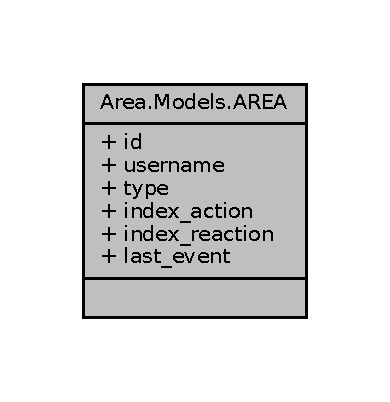
\includegraphics[width=187pt]{classArea_1_1Models_1_1AREA__coll__graph}
\end{center}
\end{figure}
\subsection*{Properties}
\begin{DoxyCompactItemize}
\item 
int \mbox{\hyperlink{classArea_1_1Models_1_1AREA_acdb37c953e13ce786f7874a002f7d4c3}{id}}\hspace{0.3cm}{\ttfamily  \mbox{[}get, set\mbox{]}}
\item 
string \mbox{\hyperlink{classArea_1_1Models_1_1AREA_ac0f022aa1dd982291b6a25e9c8fd1732}{username}}\hspace{0.3cm}{\ttfamily  \mbox{[}get, set\mbox{]}}
\item 
int \mbox{\hyperlink{classArea_1_1Models_1_1AREA_a5dbfb81ef3d8489d0d8ad2f7b0399a3f}{type}}\hspace{0.3cm}{\ttfamily  \mbox{[}get, set\mbox{]}}
\item 
int \mbox{\hyperlink{classArea_1_1Models_1_1AREA_a54de1028b1fce5e2691525f41fdf34f6}{index\+\_\+action}}\hspace{0.3cm}{\ttfamily  \mbox{[}get, set\mbox{]}}
\item 
int \mbox{\hyperlink{classArea_1_1Models_1_1AREA_a7af867d0050d70d412f932f770fb9f73}{index\+\_\+reaction}}\hspace{0.3cm}{\ttfamily  \mbox{[}get, set\mbox{]}}
\item 
string \mbox{\hyperlink{classArea_1_1Models_1_1AREA_aed4dc50ec4a309e0547d67fe378cde38}{last\+\_\+event}}\hspace{0.3cm}{\ttfamily  \mbox{[}get, set\mbox{]}}
\end{DoxyCompactItemize}


\subsection{Property Documentation}
\mbox{\Hypertarget{classArea_1_1Models_1_1AREA_acdb37c953e13ce786f7874a002f7d4c3}\label{classArea_1_1Models_1_1AREA_acdb37c953e13ce786f7874a002f7d4c3}} 
\index{Area\+::\+Models\+::\+A\+R\+EA@{Area\+::\+Models\+::\+A\+R\+EA}!id@{id}}
\index{id@{id}!Area\+::\+Models\+::\+A\+R\+EA@{Area\+::\+Models\+::\+A\+R\+EA}}
\subsubsection{\texorpdfstring{id}{id}}
{\footnotesize\ttfamily int Area.\+Models.\+A\+R\+E\+A.\+id\hspace{0.3cm}{\ttfamily [get]}, {\ttfamily [set]}}

\mbox{\Hypertarget{classArea_1_1Models_1_1AREA_a54de1028b1fce5e2691525f41fdf34f6}\label{classArea_1_1Models_1_1AREA_a54de1028b1fce5e2691525f41fdf34f6}} 
\index{Area\+::\+Models\+::\+A\+R\+EA@{Area\+::\+Models\+::\+A\+R\+EA}!index\+\_\+action@{index\+\_\+action}}
\index{index\+\_\+action@{index\+\_\+action}!Area\+::\+Models\+::\+A\+R\+EA@{Area\+::\+Models\+::\+A\+R\+EA}}
\subsubsection{\texorpdfstring{index\+\_\+action}{index\_action}}
{\footnotesize\ttfamily int Area.\+Models.\+A\+R\+E\+A.\+index\+\_\+action\hspace{0.3cm}{\ttfamily [get]}, {\ttfamily [set]}}

\mbox{\Hypertarget{classArea_1_1Models_1_1AREA_a7af867d0050d70d412f932f770fb9f73}\label{classArea_1_1Models_1_1AREA_a7af867d0050d70d412f932f770fb9f73}} 
\index{Area\+::\+Models\+::\+A\+R\+EA@{Area\+::\+Models\+::\+A\+R\+EA}!index\+\_\+reaction@{index\+\_\+reaction}}
\index{index\+\_\+reaction@{index\+\_\+reaction}!Area\+::\+Models\+::\+A\+R\+EA@{Area\+::\+Models\+::\+A\+R\+EA}}
\subsubsection{\texorpdfstring{index\+\_\+reaction}{index\_reaction}}
{\footnotesize\ttfamily int Area.\+Models.\+A\+R\+E\+A.\+index\+\_\+reaction\hspace{0.3cm}{\ttfamily [get]}, {\ttfamily [set]}}

\mbox{\Hypertarget{classArea_1_1Models_1_1AREA_aed4dc50ec4a309e0547d67fe378cde38}\label{classArea_1_1Models_1_1AREA_aed4dc50ec4a309e0547d67fe378cde38}} 
\index{Area\+::\+Models\+::\+A\+R\+EA@{Area\+::\+Models\+::\+A\+R\+EA}!last\+\_\+event@{last\+\_\+event}}
\index{last\+\_\+event@{last\+\_\+event}!Area\+::\+Models\+::\+A\+R\+EA@{Area\+::\+Models\+::\+A\+R\+EA}}
\subsubsection{\texorpdfstring{last\+\_\+event}{last\_event}}
{\footnotesize\ttfamily string Area.\+Models.\+A\+R\+E\+A.\+last\+\_\+event\hspace{0.3cm}{\ttfamily [get]}, {\ttfamily [set]}}

\mbox{\Hypertarget{classArea_1_1Models_1_1AREA_a5dbfb81ef3d8489d0d8ad2f7b0399a3f}\label{classArea_1_1Models_1_1AREA_a5dbfb81ef3d8489d0d8ad2f7b0399a3f}} 
\index{Area\+::\+Models\+::\+A\+R\+EA@{Area\+::\+Models\+::\+A\+R\+EA}!type@{type}}
\index{type@{type}!Area\+::\+Models\+::\+A\+R\+EA@{Area\+::\+Models\+::\+A\+R\+EA}}
\subsubsection{\texorpdfstring{type}{type}}
{\footnotesize\ttfamily int Area.\+Models.\+A\+R\+E\+A.\+type\hspace{0.3cm}{\ttfamily [get]}, {\ttfamily [set]}}

\mbox{\Hypertarget{classArea_1_1Models_1_1AREA_ac0f022aa1dd982291b6a25e9c8fd1732}\label{classArea_1_1Models_1_1AREA_ac0f022aa1dd982291b6a25e9c8fd1732}} 
\index{Area\+::\+Models\+::\+A\+R\+EA@{Area\+::\+Models\+::\+A\+R\+EA}!username@{username}}
\index{username@{username}!Area\+::\+Models\+::\+A\+R\+EA@{Area\+::\+Models\+::\+A\+R\+EA}}
\subsubsection{\texorpdfstring{username}{username}}
{\footnotesize\ttfamily string Area.\+Models.\+A\+R\+E\+A.\+username\hspace{0.3cm}{\ttfamily [get]}, {\ttfamily [set]}}



The documentation for this class was generated from the following file\+:\begin{DoxyCompactItemize}
\item 
Models/\+Areas/\mbox{\hyperlink{Area_8cs}{Area.\+cs}}\end{DoxyCompactItemize}

\hypertarget{classArea_1_1DAT_1_1AreaDbContext}{}\section{Area.\+D\+A\+T.\+Area\+Db\+Context Class Reference}
\label{classArea_1_1DAT_1_1AreaDbContext}\index{Area.\+D\+A\+T.\+Area\+Db\+Context@{Area.\+D\+A\+T.\+Area\+Db\+Context}}


Inheritance diagram for Area.\+D\+A\+T.\+Area\+Db\+Context\+:
\nopagebreak
\begin{figure}[H]
\begin{center}
\leavevmode
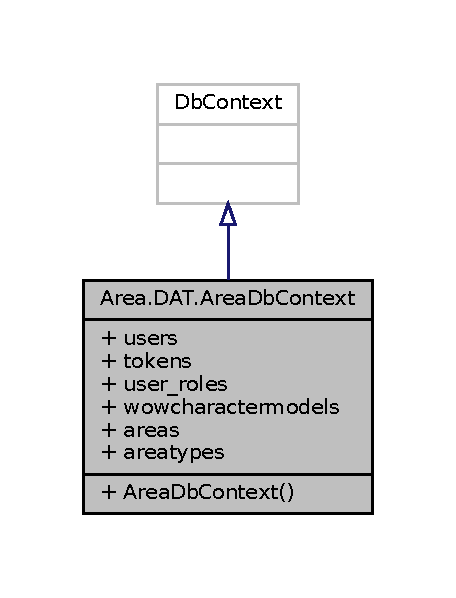
\includegraphics[width=219pt]{classArea_1_1DAT_1_1AreaDbContext__inherit__graph}
\end{center}
\end{figure}


Collaboration diagram for Area.\+D\+A\+T.\+Area\+Db\+Context\+:
\nopagebreak
\begin{figure}[H]
\begin{center}
\leavevmode
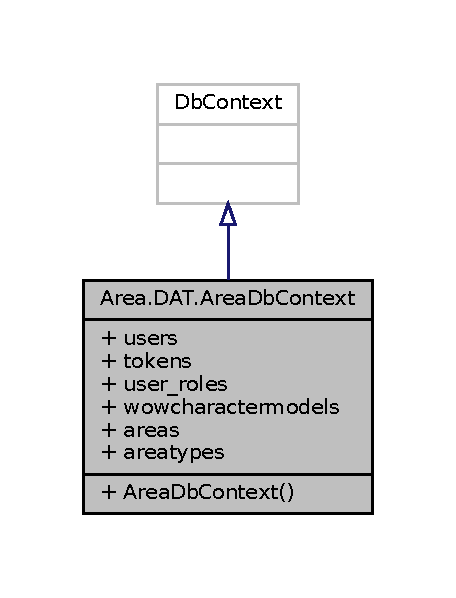
\includegraphics[width=219pt]{classArea_1_1DAT_1_1AreaDbContext__coll__graph}
\end{center}
\end{figure}
\subsection*{Public Member Functions}
\begin{DoxyCompactItemize}
\item 
\mbox{\hyperlink{classArea_1_1DAT_1_1AreaDbContext_ae24424bd38ef16488f7cfe83cff8a01d}{Area\+Db\+Context}} (Db\+Context\+Options$<$ \mbox{\hyperlink{classArea_1_1DAT_1_1AreaDbContext}{Area\+Db\+Context}} $>$ opt)
\end{DoxyCompactItemize}
\subsection*{Properties}
\begin{DoxyCompactItemize}
\item 
Db\+Set$<$ \mbox{\hyperlink{classArea_1_1Models_1_1User}{User}} $>$ \mbox{\hyperlink{classArea_1_1DAT_1_1AreaDbContext_a70a40f34149640aa8dad936e92d94147}{users}}\hspace{0.3cm}{\ttfamily  \mbox{[}get, set\mbox{]}}
\item 
Db\+Set$<$ \mbox{\hyperlink{classArea_1_1Models_1_1Token}{Token}} $>$ \mbox{\hyperlink{classArea_1_1DAT_1_1AreaDbContext_a57bfbc12f404c1d6665a8d9f59bfa635}{tokens}}\hspace{0.3cm}{\ttfamily  \mbox{[}get, set\mbox{]}}
\item 
Db\+Set$<$ \mbox{\hyperlink{classArea_1_1Models_1_1User__role}{User\+\_\+role}} $>$ \mbox{\hyperlink{classArea_1_1DAT_1_1AreaDbContext_aadce9e078963a91065c5f084dcc4656c}{user\+\_\+roles}}\hspace{0.3cm}{\ttfamily  \mbox{[}get, set\mbox{]}}
\item 
Db\+Set$<$ \mbox{\hyperlink{classArea_1_1Models_1_1WoWCharacterModel}{Wo\+W\+Character\+Model}} $>$ \mbox{\hyperlink{classArea_1_1DAT_1_1AreaDbContext_a6774df51b409ffb5ee27bf29186d4fe9}{wowcharactermodels}}\hspace{0.3cm}{\ttfamily  \mbox{[}get, set\mbox{]}}
\item 
Db\+Set$<$ \mbox{\hyperlink{classArea_1_1Models_1_1AREA}{A\+R\+EA}} $>$ \mbox{\hyperlink{classArea_1_1DAT_1_1AreaDbContext_aa049cce613ea239b90deb127916071e2}{areas}}\hspace{0.3cm}{\ttfamily  \mbox{[}get, set\mbox{]}}
\item 
Db\+Set$<$ \mbox{\hyperlink{classArea_1_1Models_1_1AreaType}{Area\+Type}} $>$ \mbox{\hyperlink{classArea_1_1DAT_1_1AreaDbContext_a2bf4466a5d72833e650cb3674e63e30c}{areatypes}}\hspace{0.3cm}{\ttfamily  \mbox{[}get, set\mbox{]}}
\end{DoxyCompactItemize}


\subsection{Constructor \& Destructor Documentation}
\mbox{\Hypertarget{classArea_1_1DAT_1_1AreaDbContext_ae24424bd38ef16488f7cfe83cff8a01d}\label{classArea_1_1DAT_1_1AreaDbContext_ae24424bd38ef16488f7cfe83cff8a01d}} 
\index{Area\+::\+D\+A\+T\+::\+Area\+Db\+Context@{Area\+::\+D\+A\+T\+::\+Area\+Db\+Context}!Area\+Db\+Context@{Area\+Db\+Context}}
\index{Area\+Db\+Context@{Area\+Db\+Context}!Area\+::\+D\+A\+T\+::\+Area\+Db\+Context@{Area\+::\+D\+A\+T\+::\+Area\+Db\+Context}}
\subsubsection{\texorpdfstring{Area\+Db\+Context()}{AreaDbContext()}}
{\footnotesize\ttfamily Area.\+D\+A\+T.\+Area\+Db\+Context.\+Area\+Db\+Context (\begin{DoxyParamCaption}\item[{Db\+Context\+Options$<$ \mbox{\hyperlink{classArea_1_1DAT_1_1AreaDbContext}{Area\+Db\+Context}} $>$}]{opt }\end{DoxyParamCaption})\hspace{0.3cm}{\ttfamily [inline]}}



\subsection{Property Documentation}
\mbox{\Hypertarget{classArea_1_1DAT_1_1AreaDbContext_aa049cce613ea239b90deb127916071e2}\label{classArea_1_1DAT_1_1AreaDbContext_aa049cce613ea239b90deb127916071e2}} 
\index{Area\+::\+D\+A\+T\+::\+Area\+Db\+Context@{Area\+::\+D\+A\+T\+::\+Area\+Db\+Context}!areas@{areas}}
\index{areas@{areas}!Area\+::\+D\+A\+T\+::\+Area\+Db\+Context@{Area\+::\+D\+A\+T\+::\+Area\+Db\+Context}}
\subsubsection{\texorpdfstring{areas}{areas}}
{\footnotesize\ttfamily Db\+Set$<$\mbox{\hyperlink{classArea_1_1Models_1_1AREA}{A\+R\+EA}}$>$ Area.\+D\+A\+T.\+Area\+Db\+Context.\+areas\hspace{0.3cm}{\ttfamily [get]}, {\ttfamily [set]}}

\mbox{\Hypertarget{classArea_1_1DAT_1_1AreaDbContext_a2bf4466a5d72833e650cb3674e63e30c}\label{classArea_1_1DAT_1_1AreaDbContext_a2bf4466a5d72833e650cb3674e63e30c}} 
\index{Area\+::\+D\+A\+T\+::\+Area\+Db\+Context@{Area\+::\+D\+A\+T\+::\+Area\+Db\+Context}!areatypes@{areatypes}}
\index{areatypes@{areatypes}!Area\+::\+D\+A\+T\+::\+Area\+Db\+Context@{Area\+::\+D\+A\+T\+::\+Area\+Db\+Context}}
\subsubsection{\texorpdfstring{areatypes}{areatypes}}
{\footnotesize\ttfamily Db\+Set$<$\mbox{\hyperlink{classArea_1_1Models_1_1AreaType}{Area\+Type}}$>$ Area.\+D\+A\+T.\+Area\+Db\+Context.\+areatypes\hspace{0.3cm}{\ttfamily [get]}, {\ttfamily [set]}}

\mbox{\Hypertarget{classArea_1_1DAT_1_1AreaDbContext_a57bfbc12f404c1d6665a8d9f59bfa635}\label{classArea_1_1DAT_1_1AreaDbContext_a57bfbc12f404c1d6665a8d9f59bfa635}} 
\index{Area\+::\+D\+A\+T\+::\+Area\+Db\+Context@{Area\+::\+D\+A\+T\+::\+Area\+Db\+Context}!tokens@{tokens}}
\index{tokens@{tokens}!Area\+::\+D\+A\+T\+::\+Area\+Db\+Context@{Area\+::\+D\+A\+T\+::\+Area\+Db\+Context}}
\subsubsection{\texorpdfstring{tokens}{tokens}}
{\footnotesize\ttfamily Db\+Set$<$\mbox{\hyperlink{classArea_1_1Models_1_1Token}{Token}}$>$ Area.\+D\+A\+T.\+Area\+Db\+Context.\+tokens\hspace{0.3cm}{\ttfamily [get]}, {\ttfamily [set]}}

\mbox{\Hypertarget{classArea_1_1DAT_1_1AreaDbContext_aadce9e078963a91065c5f084dcc4656c}\label{classArea_1_1DAT_1_1AreaDbContext_aadce9e078963a91065c5f084dcc4656c}} 
\index{Area\+::\+D\+A\+T\+::\+Area\+Db\+Context@{Area\+::\+D\+A\+T\+::\+Area\+Db\+Context}!user\+\_\+roles@{user\+\_\+roles}}
\index{user\+\_\+roles@{user\+\_\+roles}!Area\+::\+D\+A\+T\+::\+Area\+Db\+Context@{Area\+::\+D\+A\+T\+::\+Area\+Db\+Context}}
\subsubsection{\texorpdfstring{user\+\_\+roles}{user\_roles}}
{\footnotesize\ttfamily Db\+Set$<$\mbox{\hyperlink{classArea_1_1Models_1_1User__role}{User\+\_\+role}}$>$ Area.\+D\+A\+T.\+Area\+Db\+Context.\+user\+\_\+roles\hspace{0.3cm}{\ttfamily [get]}, {\ttfamily [set]}}

\mbox{\Hypertarget{classArea_1_1DAT_1_1AreaDbContext_a70a40f34149640aa8dad936e92d94147}\label{classArea_1_1DAT_1_1AreaDbContext_a70a40f34149640aa8dad936e92d94147}} 
\index{Area\+::\+D\+A\+T\+::\+Area\+Db\+Context@{Area\+::\+D\+A\+T\+::\+Area\+Db\+Context}!users@{users}}
\index{users@{users}!Area\+::\+D\+A\+T\+::\+Area\+Db\+Context@{Area\+::\+D\+A\+T\+::\+Area\+Db\+Context}}
\subsubsection{\texorpdfstring{users}{users}}
{\footnotesize\ttfamily Db\+Set$<$\mbox{\hyperlink{classArea_1_1Models_1_1User}{User}}$>$ Area.\+D\+A\+T.\+Area\+Db\+Context.\+users\hspace{0.3cm}{\ttfamily [get]}, {\ttfamily [set]}}

\mbox{\Hypertarget{classArea_1_1DAT_1_1AreaDbContext_a6774df51b409ffb5ee27bf29186d4fe9}\label{classArea_1_1DAT_1_1AreaDbContext_a6774df51b409ffb5ee27bf29186d4fe9}} 
\index{Area\+::\+D\+A\+T\+::\+Area\+Db\+Context@{Area\+::\+D\+A\+T\+::\+Area\+Db\+Context}!wowcharactermodels@{wowcharactermodels}}
\index{wowcharactermodels@{wowcharactermodels}!Area\+::\+D\+A\+T\+::\+Area\+Db\+Context@{Area\+::\+D\+A\+T\+::\+Area\+Db\+Context}}
\subsubsection{\texorpdfstring{wowcharactermodels}{wowcharactermodels}}
{\footnotesize\ttfamily Db\+Set$<$\mbox{\hyperlink{classArea_1_1Models_1_1WoWCharacterModel}{Wo\+W\+Character\+Model}}$>$ Area.\+D\+A\+T.\+Area\+Db\+Context.\+wowcharactermodels\hspace{0.3cm}{\ttfamily [get]}, {\ttfamily [set]}}



The documentation for this class was generated from the following file\+:\begin{DoxyCompactItemize}
\item 
D\+A\+T/\mbox{\hyperlink{AreaDbContext_8cs}{Area\+Db\+Context.\+cs}}\end{DoxyCompactItemize}

\hypertarget{classArea_1_1DAT_1_1AreaDbThreadContext}{}\section{Area.\+D\+A\+T.\+Area\+Db\+Thread\+Context Class Reference}
\label{classArea_1_1DAT_1_1AreaDbThreadContext}\index{Area.\+D\+A\+T.\+Area\+Db\+Thread\+Context@{Area.\+D\+A\+T.\+Area\+Db\+Thread\+Context}}


Inheritance diagram for Area.\+D\+A\+T.\+Area\+Db\+Thread\+Context\+:
\nopagebreak
\begin{figure}[H]
\begin{center}
\leavevmode
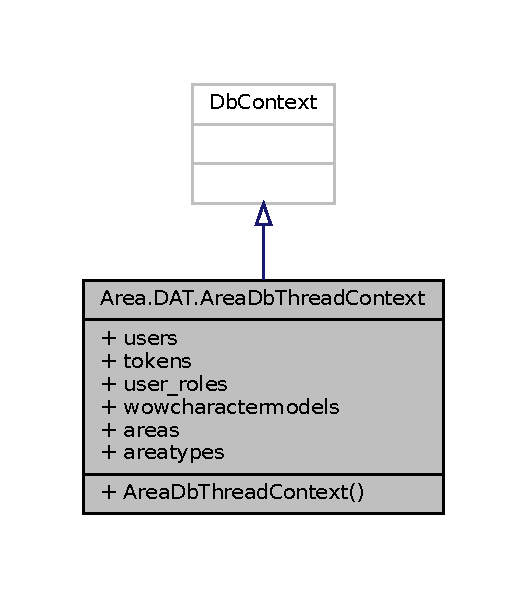
\includegraphics[width=253pt]{classArea_1_1DAT_1_1AreaDbThreadContext__inherit__graph}
\end{center}
\end{figure}


Collaboration diagram for Area.\+D\+A\+T.\+Area\+Db\+Thread\+Context\+:
\nopagebreak
\begin{figure}[H]
\begin{center}
\leavevmode
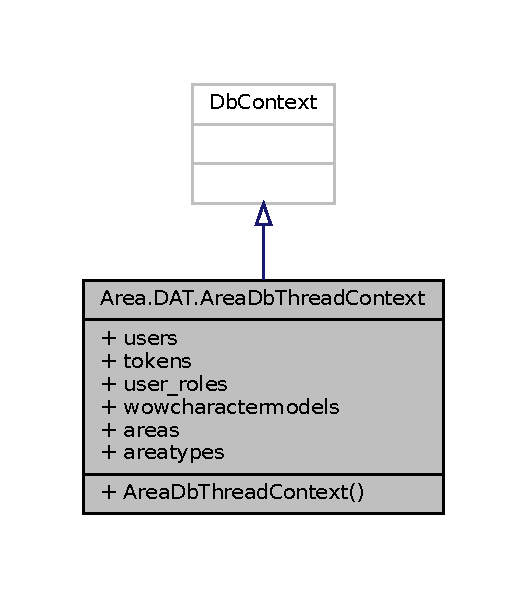
\includegraphics[width=253pt]{classArea_1_1DAT_1_1AreaDbThreadContext__coll__graph}
\end{center}
\end{figure}
\subsection*{Public Member Functions}
\begin{DoxyCompactItemize}
\item 
\mbox{\hyperlink{classArea_1_1DAT_1_1AreaDbThreadContext_ab5339ffc8ee9669ac3a13b62a622e746}{Area\+Db\+Thread\+Context}} (Db\+Context\+Options$<$ \mbox{\hyperlink{classArea_1_1DAT_1_1AreaDbThreadContext}{Area\+Db\+Thread\+Context}} $>$ opt)
\end{DoxyCompactItemize}
\subsection*{Properties}
\begin{DoxyCompactItemize}
\item 
Db\+Set$<$ \mbox{\hyperlink{classArea_1_1Models_1_1User}{User}} $>$ \mbox{\hyperlink{classArea_1_1DAT_1_1AreaDbThreadContext_a58df7d30567900ef42b1e26bfc2bbba0}{users}}\hspace{0.3cm}{\ttfamily  \mbox{[}get, set\mbox{]}}
\item 
Db\+Set$<$ \mbox{\hyperlink{classArea_1_1Models_1_1Token}{Token}} $>$ \mbox{\hyperlink{classArea_1_1DAT_1_1AreaDbThreadContext_a42fe53b25ddbc24b01c9fd2b7e81de40}{tokens}}\hspace{0.3cm}{\ttfamily  \mbox{[}get, set\mbox{]}}
\item 
Db\+Set$<$ \mbox{\hyperlink{classArea_1_1Models_1_1User__role}{User\+\_\+role}} $>$ \mbox{\hyperlink{classArea_1_1DAT_1_1AreaDbThreadContext_a371fd9e63da8effa604887e7ef010151}{user\+\_\+roles}}\hspace{0.3cm}{\ttfamily  \mbox{[}get, set\mbox{]}}
\item 
Db\+Set$<$ \mbox{\hyperlink{classArea_1_1Models_1_1WoWCharacterModel}{Wo\+W\+Character\+Model}} $>$ \mbox{\hyperlink{classArea_1_1DAT_1_1AreaDbThreadContext_ab322f4c561f0c411dd4f1b4d151e6d26}{wowcharactermodels}}\hspace{0.3cm}{\ttfamily  \mbox{[}get, set\mbox{]}}
\item 
Db\+Set$<$ \mbox{\hyperlink{classArea_1_1Models_1_1AREA}{A\+R\+EA}} $>$ \mbox{\hyperlink{classArea_1_1DAT_1_1AreaDbThreadContext_a025ba5d7d31252cdb83d49d3dcd4122f}{areas}}\hspace{0.3cm}{\ttfamily  \mbox{[}get, set\mbox{]}}
\item 
Db\+Set$<$ \mbox{\hyperlink{classArea_1_1Models_1_1AreaType}{Area\+Type}} $>$ \mbox{\hyperlink{classArea_1_1DAT_1_1AreaDbThreadContext_a30ac7d33b5e632232ae46fdc842ec349}{areatypes}}\hspace{0.3cm}{\ttfamily  \mbox{[}get, set\mbox{]}}
\end{DoxyCompactItemize}


\subsection{Constructor \& Destructor Documentation}
\mbox{\Hypertarget{classArea_1_1DAT_1_1AreaDbThreadContext_ab5339ffc8ee9669ac3a13b62a622e746}\label{classArea_1_1DAT_1_1AreaDbThreadContext_ab5339ffc8ee9669ac3a13b62a622e746}} 
\index{Area\+::\+D\+A\+T\+::\+Area\+Db\+Thread\+Context@{Area\+::\+D\+A\+T\+::\+Area\+Db\+Thread\+Context}!Area\+Db\+Thread\+Context@{Area\+Db\+Thread\+Context}}
\index{Area\+Db\+Thread\+Context@{Area\+Db\+Thread\+Context}!Area\+::\+D\+A\+T\+::\+Area\+Db\+Thread\+Context@{Area\+::\+D\+A\+T\+::\+Area\+Db\+Thread\+Context}}
\subsubsection{\texorpdfstring{Area\+Db\+Thread\+Context()}{AreaDbThreadContext()}}
{\footnotesize\ttfamily Area.\+D\+A\+T.\+Area\+Db\+Thread\+Context.\+Area\+Db\+Thread\+Context (\begin{DoxyParamCaption}\item[{Db\+Context\+Options$<$ \mbox{\hyperlink{classArea_1_1DAT_1_1AreaDbThreadContext}{Area\+Db\+Thread\+Context}} $>$}]{opt }\end{DoxyParamCaption})\hspace{0.3cm}{\ttfamily [inline]}}



\subsection{Property Documentation}
\mbox{\Hypertarget{classArea_1_1DAT_1_1AreaDbThreadContext_a025ba5d7d31252cdb83d49d3dcd4122f}\label{classArea_1_1DAT_1_1AreaDbThreadContext_a025ba5d7d31252cdb83d49d3dcd4122f}} 
\index{Area\+::\+D\+A\+T\+::\+Area\+Db\+Thread\+Context@{Area\+::\+D\+A\+T\+::\+Area\+Db\+Thread\+Context}!areas@{areas}}
\index{areas@{areas}!Area\+::\+D\+A\+T\+::\+Area\+Db\+Thread\+Context@{Area\+::\+D\+A\+T\+::\+Area\+Db\+Thread\+Context}}
\subsubsection{\texorpdfstring{areas}{areas}}
{\footnotesize\ttfamily Db\+Set$<$\mbox{\hyperlink{classArea_1_1Models_1_1AREA}{A\+R\+EA}}$>$ Area.\+D\+A\+T.\+Area\+Db\+Thread\+Context.\+areas\hspace{0.3cm}{\ttfamily [get]}, {\ttfamily [set]}}

\mbox{\Hypertarget{classArea_1_1DAT_1_1AreaDbThreadContext_a30ac7d33b5e632232ae46fdc842ec349}\label{classArea_1_1DAT_1_1AreaDbThreadContext_a30ac7d33b5e632232ae46fdc842ec349}} 
\index{Area\+::\+D\+A\+T\+::\+Area\+Db\+Thread\+Context@{Area\+::\+D\+A\+T\+::\+Area\+Db\+Thread\+Context}!areatypes@{areatypes}}
\index{areatypes@{areatypes}!Area\+::\+D\+A\+T\+::\+Area\+Db\+Thread\+Context@{Area\+::\+D\+A\+T\+::\+Area\+Db\+Thread\+Context}}
\subsubsection{\texorpdfstring{areatypes}{areatypes}}
{\footnotesize\ttfamily Db\+Set$<$\mbox{\hyperlink{classArea_1_1Models_1_1AreaType}{Area\+Type}}$>$ Area.\+D\+A\+T.\+Area\+Db\+Thread\+Context.\+areatypes\hspace{0.3cm}{\ttfamily [get]}, {\ttfamily [set]}}

\mbox{\Hypertarget{classArea_1_1DAT_1_1AreaDbThreadContext_a42fe53b25ddbc24b01c9fd2b7e81de40}\label{classArea_1_1DAT_1_1AreaDbThreadContext_a42fe53b25ddbc24b01c9fd2b7e81de40}} 
\index{Area\+::\+D\+A\+T\+::\+Area\+Db\+Thread\+Context@{Area\+::\+D\+A\+T\+::\+Area\+Db\+Thread\+Context}!tokens@{tokens}}
\index{tokens@{tokens}!Area\+::\+D\+A\+T\+::\+Area\+Db\+Thread\+Context@{Area\+::\+D\+A\+T\+::\+Area\+Db\+Thread\+Context}}
\subsubsection{\texorpdfstring{tokens}{tokens}}
{\footnotesize\ttfamily Db\+Set$<$\mbox{\hyperlink{classArea_1_1Models_1_1Token}{Token}}$>$ Area.\+D\+A\+T.\+Area\+Db\+Thread\+Context.\+tokens\hspace{0.3cm}{\ttfamily [get]}, {\ttfamily [set]}}

\mbox{\Hypertarget{classArea_1_1DAT_1_1AreaDbThreadContext_a371fd9e63da8effa604887e7ef010151}\label{classArea_1_1DAT_1_1AreaDbThreadContext_a371fd9e63da8effa604887e7ef010151}} 
\index{Area\+::\+D\+A\+T\+::\+Area\+Db\+Thread\+Context@{Area\+::\+D\+A\+T\+::\+Area\+Db\+Thread\+Context}!user\+\_\+roles@{user\+\_\+roles}}
\index{user\+\_\+roles@{user\+\_\+roles}!Area\+::\+D\+A\+T\+::\+Area\+Db\+Thread\+Context@{Area\+::\+D\+A\+T\+::\+Area\+Db\+Thread\+Context}}
\subsubsection{\texorpdfstring{user\+\_\+roles}{user\_roles}}
{\footnotesize\ttfamily Db\+Set$<$\mbox{\hyperlink{classArea_1_1Models_1_1User__role}{User\+\_\+role}}$>$ Area.\+D\+A\+T.\+Area\+Db\+Thread\+Context.\+user\+\_\+roles\hspace{0.3cm}{\ttfamily [get]}, {\ttfamily [set]}}

\mbox{\Hypertarget{classArea_1_1DAT_1_1AreaDbThreadContext_a58df7d30567900ef42b1e26bfc2bbba0}\label{classArea_1_1DAT_1_1AreaDbThreadContext_a58df7d30567900ef42b1e26bfc2bbba0}} 
\index{Area\+::\+D\+A\+T\+::\+Area\+Db\+Thread\+Context@{Area\+::\+D\+A\+T\+::\+Area\+Db\+Thread\+Context}!users@{users}}
\index{users@{users}!Area\+::\+D\+A\+T\+::\+Area\+Db\+Thread\+Context@{Area\+::\+D\+A\+T\+::\+Area\+Db\+Thread\+Context}}
\subsubsection{\texorpdfstring{users}{users}}
{\footnotesize\ttfamily Db\+Set$<$\mbox{\hyperlink{classArea_1_1Models_1_1User}{User}}$>$ Area.\+D\+A\+T.\+Area\+Db\+Thread\+Context.\+users\hspace{0.3cm}{\ttfamily [get]}, {\ttfamily [set]}}

\mbox{\Hypertarget{classArea_1_1DAT_1_1AreaDbThreadContext_ab322f4c561f0c411dd4f1b4d151e6d26}\label{classArea_1_1DAT_1_1AreaDbThreadContext_ab322f4c561f0c411dd4f1b4d151e6d26}} 
\index{Area\+::\+D\+A\+T\+::\+Area\+Db\+Thread\+Context@{Area\+::\+D\+A\+T\+::\+Area\+Db\+Thread\+Context}!wowcharactermodels@{wowcharactermodels}}
\index{wowcharactermodels@{wowcharactermodels}!Area\+::\+D\+A\+T\+::\+Area\+Db\+Thread\+Context@{Area\+::\+D\+A\+T\+::\+Area\+Db\+Thread\+Context}}
\subsubsection{\texorpdfstring{wowcharactermodels}{wowcharactermodels}}
{\footnotesize\ttfamily Db\+Set$<$\mbox{\hyperlink{classArea_1_1Models_1_1WoWCharacterModel}{Wo\+W\+Character\+Model}}$>$ Area.\+D\+A\+T.\+Area\+Db\+Thread\+Context.\+wowcharactermodels\hspace{0.3cm}{\ttfamily [get]}, {\ttfamily [set]}}



The documentation for this class was generated from the following file\+:\begin{DoxyCompactItemize}
\item 
D\+A\+T/\mbox{\hyperlink{AreaDbContext_8cs}{Area\+Db\+Context.\+cs}}\end{DoxyCompactItemize}

\hypertarget{classArea_1_1Models_1_1AreaFactory}{}\section{Area.\+Models.\+Area\+Factory Class Reference}
\label{classArea_1_1Models_1_1AreaFactory}\index{Area.\+Models.\+Area\+Factory@{Area.\+Models.\+Area\+Factory}}


Collaboration diagram for Area.\+Models.\+Area\+Factory\+:
\nopagebreak
\begin{figure}[H]
\begin{center}
\leavevmode
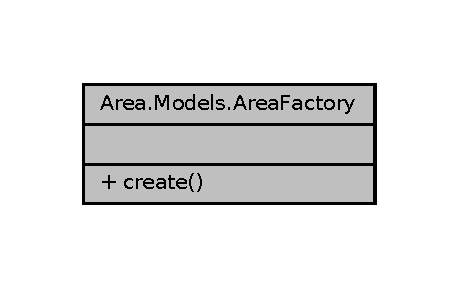
\includegraphics[width=220pt]{classArea_1_1Models_1_1AreaFactory__coll__graph}
\end{center}
\end{figure}
\subsection*{Static Public Member Functions}
\begin{DoxyCompactItemize}
\item 
static \mbox{\hyperlink{interfaceArea_1_1Models_1_1IArea}{I\+Area}} \mbox{\hyperlink{classArea_1_1Models_1_1AreaFactory_a39c7070acc78dddbde39b9e12df26c3d}{create}} (\mbox{\hyperlink{classArea_1_1Models_1_1AREA}{A\+R\+EA}} area, \mbox{\hyperlink{classArea_1_1DAT_1_1AreaDbContext}{Area\+Db\+Context}} DB)
\end{DoxyCompactItemize}


\subsection{Member Function Documentation}
\mbox{\Hypertarget{classArea_1_1Models_1_1AreaFactory_a39c7070acc78dddbde39b9e12df26c3d}\label{classArea_1_1Models_1_1AreaFactory_a39c7070acc78dddbde39b9e12df26c3d}} 
\index{Area\+::\+Models\+::\+Area\+Factory@{Area\+::\+Models\+::\+Area\+Factory}!create@{create}}
\index{create@{create}!Area\+::\+Models\+::\+Area\+Factory@{Area\+::\+Models\+::\+Area\+Factory}}
\subsubsection{\texorpdfstring{create()}{create()}}
{\footnotesize\ttfamily static \mbox{\hyperlink{interfaceArea_1_1Models_1_1IArea}{I\+Area}} Area.\+Models.\+Area\+Factory.\+create (\begin{DoxyParamCaption}\item[{\mbox{\hyperlink{classArea_1_1Models_1_1AREA}{A\+R\+EA}}}]{area,  }\item[{\mbox{\hyperlink{classArea_1_1DAT_1_1AreaDbContext}{Area\+Db\+Context}}}]{DB }\end{DoxyParamCaption})\hspace{0.3cm}{\ttfamily [inline]}, {\ttfamily [static]}}



The documentation for this class was generated from the following file\+:\begin{DoxyCompactItemize}
\item 
Models/\+Areas/\mbox{\hyperlink{AreaFactory_8cs}{Area\+Factory.\+cs}}\end{DoxyCompactItemize}

\hypertarget{classArea_1_1Models_1_1AreaType}{}\section{Area.\+Models.\+Area\+Type Class Reference}
\label{classArea_1_1Models_1_1AreaType}\index{Area.\+Models.\+Area\+Type@{Area.\+Models.\+Area\+Type}}


Collaboration diagram for Area.\+Models.\+Area\+Type\+:
\nopagebreak
\begin{figure}[H]
\begin{center}
\leavevmode
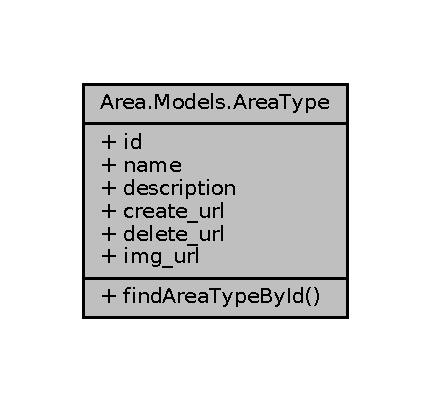
\includegraphics[width=207pt]{classArea_1_1Models_1_1AreaType__coll__graph}
\end{center}
\end{figure}
\subsection*{Static Public Member Functions}
\begin{DoxyCompactItemize}
\item 
static \mbox{\hyperlink{classArea_1_1Models_1_1AreaType}{Area\+Type}} \mbox{\hyperlink{classArea_1_1Models_1_1AreaType_a06f11a87a3ffb86fe075d5db4bba48b2}{find\+Area\+Type\+By\+Id}} (\mbox{\hyperlink{classArea_1_1DAT_1_1AreaDbContext}{Area\+Db\+Context}} DB, int \mbox{\hyperlink{classArea_1_1Models_1_1AreaType_a334470e1882a0d27aad7dc0a180e5b0b}{id}})
\end{DoxyCompactItemize}
\subsection*{Properties}
\begin{DoxyCompactItemize}
\item 
int \mbox{\hyperlink{classArea_1_1Models_1_1AreaType_a334470e1882a0d27aad7dc0a180e5b0b}{id}}\hspace{0.3cm}{\ttfamily  \mbox{[}get, set\mbox{]}}
\item 
string \mbox{\hyperlink{classArea_1_1Models_1_1AreaType_a96fa53a9c8d977d9a3afa7e501a862fa}{name}}\hspace{0.3cm}{\ttfamily  \mbox{[}get, set\mbox{]}}
\item 
string \mbox{\hyperlink{classArea_1_1Models_1_1AreaType_a9e4921cb37dd5d3eca61455c28f399b0}{description}}\hspace{0.3cm}{\ttfamily  \mbox{[}get, set\mbox{]}}
\item 
string \mbox{\hyperlink{classArea_1_1Models_1_1AreaType_a57a0e360895801c2f41c626d27becc17}{create\+\_\+url}}\hspace{0.3cm}{\ttfamily  \mbox{[}get, set\mbox{]}}
\item 
string \mbox{\hyperlink{classArea_1_1Models_1_1AreaType_a5714a6004dd5fab7a60158bfcb609da8}{delete\+\_\+url}}\hspace{0.3cm}{\ttfamily  \mbox{[}get, set\mbox{]}}
\item 
string \mbox{\hyperlink{classArea_1_1Models_1_1AreaType_a3db4de9d040e34f86dde99b0ecb10093}{img\+\_\+url}}\hspace{0.3cm}{\ttfamily  \mbox{[}get, set\mbox{]}}
\end{DoxyCompactItemize}


\subsection{Member Function Documentation}
\mbox{\Hypertarget{classArea_1_1Models_1_1AreaType_a06f11a87a3ffb86fe075d5db4bba48b2}\label{classArea_1_1Models_1_1AreaType_a06f11a87a3ffb86fe075d5db4bba48b2}} 
\index{Area\+::\+Models\+::\+Area\+Type@{Area\+::\+Models\+::\+Area\+Type}!find\+Area\+Type\+By\+Id@{find\+Area\+Type\+By\+Id}}
\index{find\+Area\+Type\+By\+Id@{find\+Area\+Type\+By\+Id}!Area\+::\+Models\+::\+Area\+Type@{Area\+::\+Models\+::\+Area\+Type}}
\subsubsection{\texorpdfstring{find\+Area\+Type\+By\+Id()}{findAreaTypeById()}}
{\footnotesize\ttfamily static \mbox{\hyperlink{classArea_1_1Models_1_1AreaType}{Area\+Type}} Area.\+Models.\+Area\+Type.\+find\+Area\+Type\+By\+Id (\begin{DoxyParamCaption}\item[{\mbox{\hyperlink{classArea_1_1DAT_1_1AreaDbContext}{Area\+Db\+Context}}}]{DB,  }\item[{int}]{id }\end{DoxyParamCaption})\hspace{0.3cm}{\ttfamily [inline]}, {\ttfamily [static]}}



\subsection{Property Documentation}
\mbox{\Hypertarget{classArea_1_1Models_1_1AreaType_a57a0e360895801c2f41c626d27becc17}\label{classArea_1_1Models_1_1AreaType_a57a0e360895801c2f41c626d27becc17}} 
\index{Area\+::\+Models\+::\+Area\+Type@{Area\+::\+Models\+::\+Area\+Type}!create\+\_\+url@{create\+\_\+url}}
\index{create\+\_\+url@{create\+\_\+url}!Area\+::\+Models\+::\+Area\+Type@{Area\+::\+Models\+::\+Area\+Type}}
\subsubsection{\texorpdfstring{create\+\_\+url}{create\_url}}
{\footnotesize\ttfamily string Area.\+Models.\+Area\+Type.\+create\+\_\+url\hspace{0.3cm}{\ttfamily [get]}, {\ttfamily [set]}}

\mbox{\Hypertarget{classArea_1_1Models_1_1AreaType_a5714a6004dd5fab7a60158bfcb609da8}\label{classArea_1_1Models_1_1AreaType_a5714a6004dd5fab7a60158bfcb609da8}} 
\index{Area\+::\+Models\+::\+Area\+Type@{Area\+::\+Models\+::\+Area\+Type}!delete\+\_\+url@{delete\+\_\+url}}
\index{delete\+\_\+url@{delete\+\_\+url}!Area\+::\+Models\+::\+Area\+Type@{Area\+::\+Models\+::\+Area\+Type}}
\subsubsection{\texorpdfstring{delete\+\_\+url}{delete\_url}}
{\footnotesize\ttfamily string Area.\+Models.\+Area\+Type.\+delete\+\_\+url\hspace{0.3cm}{\ttfamily [get]}, {\ttfamily [set]}}

\mbox{\Hypertarget{classArea_1_1Models_1_1AreaType_a9e4921cb37dd5d3eca61455c28f399b0}\label{classArea_1_1Models_1_1AreaType_a9e4921cb37dd5d3eca61455c28f399b0}} 
\index{Area\+::\+Models\+::\+Area\+Type@{Area\+::\+Models\+::\+Area\+Type}!description@{description}}
\index{description@{description}!Area\+::\+Models\+::\+Area\+Type@{Area\+::\+Models\+::\+Area\+Type}}
\subsubsection{\texorpdfstring{description}{description}}
{\footnotesize\ttfamily string Area.\+Models.\+Area\+Type.\+description\hspace{0.3cm}{\ttfamily [get]}, {\ttfamily [set]}}

\mbox{\Hypertarget{classArea_1_1Models_1_1AreaType_a334470e1882a0d27aad7dc0a180e5b0b}\label{classArea_1_1Models_1_1AreaType_a334470e1882a0d27aad7dc0a180e5b0b}} 
\index{Area\+::\+Models\+::\+Area\+Type@{Area\+::\+Models\+::\+Area\+Type}!id@{id}}
\index{id@{id}!Area\+::\+Models\+::\+Area\+Type@{Area\+::\+Models\+::\+Area\+Type}}
\subsubsection{\texorpdfstring{id}{id}}
{\footnotesize\ttfamily int Area.\+Models.\+Area\+Type.\+id\hspace{0.3cm}{\ttfamily [get]}, {\ttfamily [set]}}

\mbox{\Hypertarget{classArea_1_1Models_1_1AreaType_a3db4de9d040e34f86dde99b0ecb10093}\label{classArea_1_1Models_1_1AreaType_a3db4de9d040e34f86dde99b0ecb10093}} 
\index{Area\+::\+Models\+::\+Area\+Type@{Area\+::\+Models\+::\+Area\+Type}!img\+\_\+url@{img\+\_\+url}}
\index{img\+\_\+url@{img\+\_\+url}!Area\+::\+Models\+::\+Area\+Type@{Area\+::\+Models\+::\+Area\+Type}}
\subsubsection{\texorpdfstring{img\+\_\+url}{img\_url}}
{\footnotesize\ttfamily string Area.\+Models.\+Area\+Type.\+img\+\_\+url\hspace{0.3cm}{\ttfamily [get]}, {\ttfamily [set]}}

\mbox{\Hypertarget{classArea_1_1Models_1_1AreaType_a96fa53a9c8d977d9a3afa7e501a862fa}\label{classArea_1_1Models_1_1AreaType_a96fa53a9c8d977d9a3afa7e501a862fa}} 
\index{Area\+::\+Models\+::\+Area\+Type@{Area\+::\+Models\+::\+Area\+Type}!name@{name}}
\index{name@{name}!Area\+::\+Models\+::\+Area\+Type@{Area\+::\+Models\+::\+Area\+Type}}
\subsubsection{\texorpdfstring{name}{name}}
{\footnotesize\ttfamily string Area.\+Models.\+Area\+Type.\+name\hspace{0.3cm}{\ttfamily [get]}, {\ttfamily [set]}}



The documentation for this class was generated from the following file\+:\begin{DoxyCompactItemize}
\item 
Models/\+Areas/\mbox{\hyperlink{AreaType_8cs}{Area\+Type.\+cs}}\end{DoxyCompactItemize}

\hypertarget{classArea_1_1Controllers_1_1ClientGmail}{}\section{Area.\+Controllers.\+Client\+Gmail Class Reference}
\label{classArea_1_1Controllers_1_1ClientGmail}\index{Area.\+Controllers.\+Client\+Gmail@{Area.\+Controllers.\+Client\+Gmail}}


Collaboration diagram for Area.\+Controllers.\+Client\+Gmail\+:
\nopagebreak
\begin{figure}[H]
\begin{center}
\leavevmode
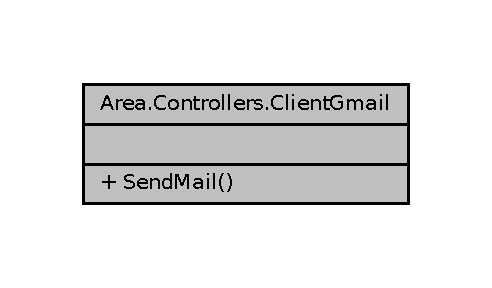
\includegraphics[width=236pt]{classArea_1_1Controllers_1_1ClientGmail__coll__graph}
\end{center}
\end{figure}
\subsection*{Public Member Functions}
\begin{DoxyCompactItemize}
\item 
void \mbox{\hyperlink{classArea_1_1Controllers_1_1ClientGmail_a647e7e52a44ff6d0e7530163f16a60ea}{Send\+Mail}} (string mail\+Addr, string code)
\end{DoxyCompactItemize}


\subsection{Member Function Documentation}
\mbox{\Hypertarget{classArea_1_1Controllers_1_1ClientGmail_a647e7e52a44ff6d0e7530163f16a60ea}\label{classArea_1_1Controllers_1_1ClientGmail_a647e7e52a44ff6d0e7530163f16a60ea}} 
\index{Area\+::\+Controllers\+::\+Client\+Gmail@{Area\+::\+Controllers\+::\+Client\+Gmail}!Send\+Mail@{Send\+Mail}}
\index{Send\+Mail@{Send\+Mail}!Area\+::\+Controllers\+::\+Client\+Gmail@{Area\+::\+Controllers\+::\+Client\+Gmail}}
\subsubsection{\texorpdfstring{Send\+Mail()}{SendMail()}}
{\footnotesize\ttfamily void Area.\+Controllers.\+Client\+Gmail.\+Send\+Mail (\begin{DoxyParamCaption}\item[{string}]{mail\+Addr,  }\item[{string}]{code }\end{DoxyParamCaption})\hspace{0.3cm}{\ttfamily [inline]}}



The documentation for this class was generated from the following file\+:\begin{DoxyCompactItemize}
\item 
Controllers/\mbox{\hyperlink{HomeController_8cs}{Home\+Controller.\+cs}}\end{DoxyCompactItemize}

\hypertarget{classArea_1_1Controllers_1_1ConnectionController}{}\section{Area.\+Controllers.\+Connection\+Controller Class Reference}
\label{classArea_1_1Controllers_1_1ConnectionController}\index{Area.\+Controllers.\+Connection\+Controller@{Area.\+Controllers.\+Connection\+Controller}}


Inheritance diagram for Area.\+Controllers.\+Connection\+Controller\+:
\nopagebreak
\begin{figure}[H]
\begin{center}
\leavevmode
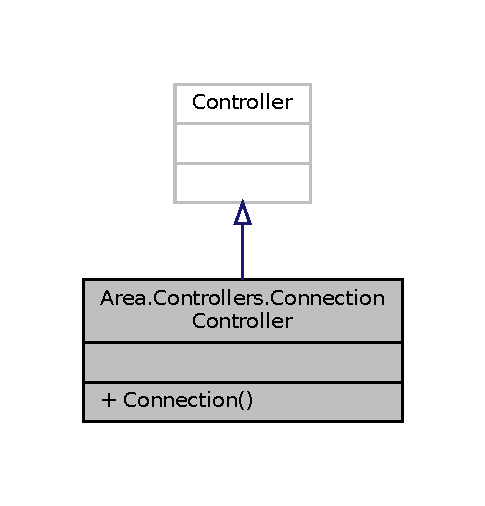
\includegraphics[width=233pt]{classArea_1_1Controllers_1_1ConnectionController__inherit__graph}
\end{center}
\end{figure}


Collaboration diagram for Area.\+Controllers.\+Connection\+Controller\+:
\nopagebreak
\begin{figure}[H]
\begin{center}
\leavevmode
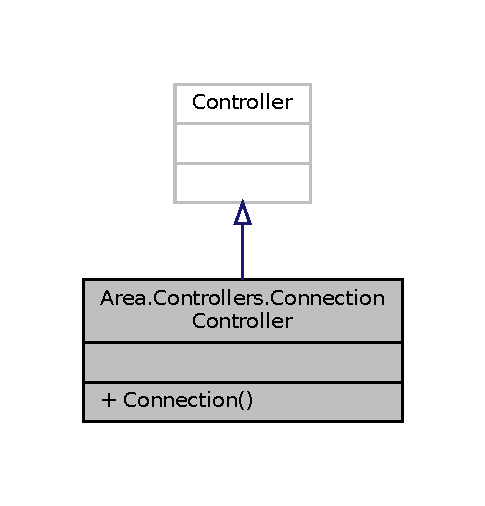
\includegraphics[width=233pt]{classArea_1_1Controllers_1_1ConnectionController__coll__graph}
\end{center}
\end{figure}
\subsection*{Public Member Functions}
\begin{DoxyCompactItemize}
\item 
Action\+Result \mbox{\hyperlink{classArea_1_1Controllers_1_1ConnectionController_a17da8a2a6e745d7c9d516e90a423c8c0}{Connection}} ()
\end{DoxyCompactItemize}


\subsection{Member Function Documentation}
\mbox{\Hypertarget{classArea_1_1Controllers_1_1ConnectionController_a17da8a2a6e745d7c9d516e90a423c8c0}\label{classArea_1_1Controllers_1_1ConnectionController_a17da8a2a6e745d7c9d516e90a423c8c0}} 
\index{Area\+::\+Controllers\+::\+Connection\+Controller@{Area\+::\+Controllers\+::\+Connection\+Controller}!Connection@{Connection}}
\index{Connection@{Connection}!Area\+::\+Controllers\+::\+Connection\+Controller@{Area\+::\+Controllers\+::\+Connection\+Controller}}
\subsubsection{\texorpdfstring{Connection()}{Connection()}}
{\footnotesize\ttfamily Action\+Result Area.\+Controllers.\+Connection\+Controller.\+Connection (\begin{DoxyParamCaption}{ }\end{DoxyParamCaption})\hspace{0.3cm}{\ttfamily [inline]}}



The documentation for this class was generated from the following file\+:\begin{DoxyCompactItemize}
\item 
Controllers/\mbox{\hyperlink{ConnectionController_8cs}{Connection\+Controller.\+cs}}\end{DoxyCompactItemize}

\hypertarget{classArea_1_1Models_1_1ErrorLog}{}\section{Area.\+Models.\+Error\+Log Class Reference}
\label{classArea_1_1Models_1_1ErrorLog}\index{Area.\+Models.\+Error\+Log@{Area.\+Models.\+Error\+Log}}


Collaboration diagram for Area.\+Models.\+Error\+Log\+:
\nopagebreak
\begin{figure}[H]
\begin{center}
\leavevmode
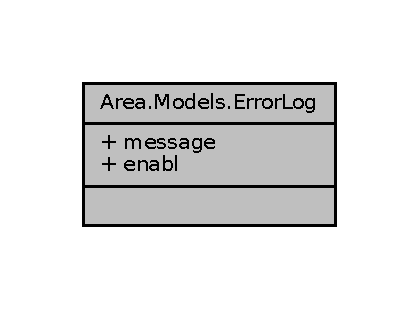
\includegraphics[width=201pt]{classArea_1_1Models_1_1ErrorLog__coll__graph}
\end{center}
\end{figure}
\subsection*{Properties}
\begin{DoxyCompactItemize}
\item 
string \mbox{\hyperlink{classArea_1_1Models_1_1ErrorLog_a0a2f2fc766e51324db7b7157c72f73cc}{message}}\hspace{0.3cm}{\ttfamily  \mbox{[}get, set\mbox{]}}
\item 
bool \mbox{\hyperlink{classArea_1_1Models_1_1ErrorLog_afc1deffe6377c972754eef679ce05473}{enabl}}\hspace{0.3cm}{\ttfamily  \mbox{[}get, set\mbox{]}}
\end{DoxyCompactItemize}


\subsection{Property Documentation}
\mbox{\Hypertarget{classArea_1_1Models_1_1ErrorLog_afc1deffe6377c972754eef679ce05473}\label{classArea_1_1Models_1_1ErrorLog_afc1deffe6377c972754eef679ce05473}} 
\index{Area\+::\+Models\+::\+Error\+Log@{Area\+::\+Models\+::\+Error\+Log}!enabl@{enabl}}
\index{enabl@{enabl}!Area\+::\+Models\+::\+Error\+Log@{Area\+::\+Models\+::\+Error\+Log}}
\subsubsection{\texorpdfstring{enabl}{enabl}}
{\footnotesize\ttfamily bool Area.\+Models.\+Error\+Log.\+enabl\hspace{0.3cm}{\ttfamily [get]}, {\ttfamily [set]}}

\mbox{\Hypertarget{classArea_1_1Models_1_1ErrorLog_a0a2f2fc766e51324db7b7157c72f73cc}\label{classArea_1_1Models_1_1ErrorLog_a0a2f2fc766e51324db7b7157c72f73cc}} 
\index{Area\+::\+Models\+::\+Error\+Log@{Area\+::\+Models\+::\+Error\+Log}!message@{message}}
\index{message@{message}!Area\+::\+Models\+::\+Error\+Log@{Area\+::\+Models\+::\+Error\+Log}}
\subsubsection{\texorpdfstring{message}{message}}
{\footnotesize\ttfamily string Area.\+Models.\+Error\+Log.\+message\hspace{0.3cm}{\ttfamily [get]}, {\ttfamily [set]}}



The documentation for this class was generated from the following file\+:\begin{DoxyCompactItemize}
\item 
Models/\mbox{\hyperlink{ErrorLog_8cs}{Error\+Log.\+cs}}\end{DoxyCompactItemize}

\hypertarget{classArea_1_1Models_1_1ErrorViewModel}{}\section{Area.\+Models.\+Error\+View\+Model Class Reference}
\label{classArea_1_1Models_1_1ErrorViewModel}\index{Area.\+Models.\+Error\+View\+Model@{Area.\+Models.\+Error\+View\+Model}}


Collaboration diagram for Area.\+Models.\+Error\+View\+Model\+:
\nopagebreak
\begin{figure}[H]
\begin{center}
\leavevmode
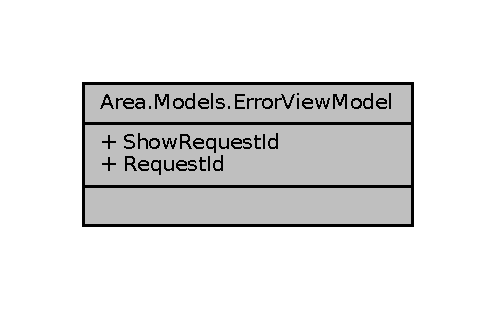
\includegraphics[width=238pt]{classArea_1_1Models_1_1ErrorViewModel__coll__graph}
\end{center}
\end{figure}
\subsection*{Public Attributes}
\begin{DoxyCompactItemize}
\item 
bool \mbox{\hyperlink{classArea_1_1Models_1_1ErrorViewModel_ae6d9b53d73e3d33702f8630c6a524881}{Show\+Request\+Id}} =$>$ !string.\+Is\+Null\+Or\+Empty(\mbox{\hyperlink{classArea_1_1Models_1_1ErrorViewModel_aef67bef86ae4e1edfc14fb486dba1981}{Request\+Id}})
\end{DoxyCompactItemize}
\subsection*{Properties}
\begin{DoxyCompactItemize}
\item 
string \mbox{\hyperlink{classArea_1_1Models_1_1ErrorViewModel_aef67bef86ae4e1edfc14fb486dba1981}{Request\+Id}}\hspace{0.3cm}{\ttfamily  \mbox{[}get, set\mbox{]}}
\end{DoxyCompactItemize}


\subsection{Member Data Documentation}
\mbox{\Hypertarget{classArea_1_1Models_1_1ErrorViewModel_ae6d9b53d73e3d33702f8630c6a524881}\label{classArea_1_1Models_1_1ErrorViewModel_ae6d9b53d73e3d33702f8630c6a524881}} 
\index{Area\+::\+Models\+::\+Error\+View\+Model@{Area\+::\+Models\+::\+Error\+View\+Model}!Show\+Request\+Id@{Show\+Request\+Id}}
\index{Show\+Request\+Id@{Show\+Request\+Id}!Area\+::\+Models\+::\+Error\+View\+Model@{Area\+::\+Models\+::\+Error\+View\+Model}}
\subsubsection{\texorpdfstring{Show\+Request\+Id}{ShowRequestId}}
{\footnotesize\ttfamily bool Area.\+Models.\+Error\+View\+Model.\+Show\+Request\+Id =$>$ !string.\+Is\+Null\+Or\+Empty(\mbox{\hyperlink{classArea_1_1Models_1_1ErrorViewModel_aef67bef86ae4e1edfc14fb486dba1981}{Request\+Id}})}



\subsection{Property Documentation}
\mbox{\Hypertarget{classArea_1_1Models_1_1ErrorViewModel_aef67bef86ae4e1edfc14fb486dba1981}\label{classArea_1_1Models_1_1ErrorViewModel_aef67bef86ae4e1edfc14fb486dba1981}} 
\index{Area\+::\+Models\+::\+Error\+View\+Model@{Area\+::\+Models\+::\+Error\+View\+Model}!Request\+Id@{Request\+Id}}
\index{Request\+Id@{Request\+Id}!Area\+::\+Models\+::\+Error\+View\+Model@{Area\+::\+Models\+::\+Error\+View\+Model}}
\subsubsection{\texorpdfstring{Request\+Id}{RequestId}}
{\footnotesize\ttfamily string Area.\+Models.\+Error\+View\+Model.\+Request\+Id\hspace{0.3cm}{\ttfamily [get]}, {\ttfamily [set]}}



The documentation for this class was generated from the following file\+:\begin{DoxyCompactItemize}
\item 
Models/\mbox{\hyperlink{ErrorViewModel_8cs}{Error\+View\+Model.\+cs}}\end{DoxyCompactItemize}

\hypertarget{classArea_1_1Controllers_1_1FacebookController}{}\section{Area.\+Controllers.\+Facebook\+Controller Class Reference}
\label{classArea_1_1Controllers_1_1FacebookController}\index{Area.\+Controllers.\+Facebook\+Controller@{Area.\+Controllers.\+Facebook\+Controller}}


Inheritance diagram for Area.\+Controllers.\+Facebook\+Controller\+:
\nopagebreak
\begin{figure}[H]
\begin{center}
\leavevmode
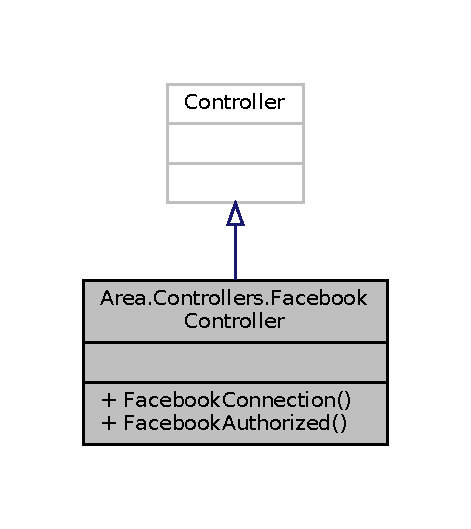
\includegraphics[width=226pt]{classArea_1_1Controllers_1_1FacebookController__inherit__graph}
\end{center}
\end{figure}


Collaboration diagram for Area.\+Controllers.\+Facebook\+Controller\+:
\nopagebreak
\begin{figure}[H]
\begin{center}
\leavevmode
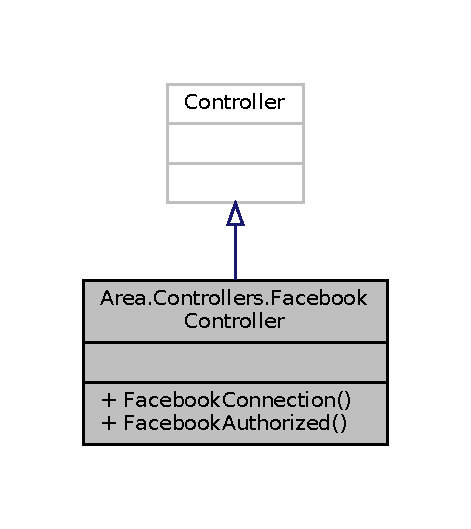
\includegraphics[width=226pt]{classArea_1_1Controllers_1_1FacebookController__coll__graph}
\end{center}
\end{figure}
\subsection*{Public Member Functions}
\begin{DoxyCompactItemize}
\item 
Action\+Result \mbox{\hyperlink{classArea_1_1Controllers_1_1FacebookController_a1218de7760311df99a293d4723414154}{Facebook\+Connection}} ()
\item 
Action\+Result \mbox{\hyperlink{classArea_1_1Controllers_1_1FacebookController_adc0a3bd0afae0028b22767eabb749e37}{Facebook\+Authorized}} (string state, string code, \mbox{[}From\+Services\mbox{]} \mbox{\hyperlink{classArea_1_1DAT_1_1AreaDbContext}{Area\+Db\+Context}} DB)
\end{DoxyCompactItemize}


\subsection{Member Function Documentation}
\mbox{\Hypertarget{classArea_1_1Controllers_1_1FacebookController_adc0a3bd0afae0028b22767eabb749e37}\label{classArea_1_1Controllers_1_1FacebookController_adc0a3bd0afae0028b22767eabb749e37}} 
\index{Area\+::\+Controllers\+::\+Facebook\+Controller@{Area\+::\+Controllers\+::\+Facebook\+Controller}!Facebook\+Authorized@{Facebook\+Authorized}}
\index{Facebook\+Authorized@{Facebook\+Authorized}!Area\+::\+Controllers\+::\+Facebook\+Controller@{Area\+::\+Controllers\+::\+Facebook\+Controller}}
\subsubsection{\texorpdfstring{Facebook\+Authorized()}{FacebookAuthorized()}}
{\footnotesize\ttfamily Action\+Result Area.\+Controllers.\+Facebook\+Controller.\+Facebook\+Authorized (\begin{DoxyParamCaption}\item[{string}]{state,  }\item[{string}]{code,  }\item[{\mbox{[}\+From\+Services\mbox{]} \mbox{\hyperlink{classArea_1_1DAT_1_1AreaDbContext}{Area\+Db\+Context}}}]{DB }\end{DoxyParamCaption})\hspace{0.3cm}{\ttfamily [inline]}}

\mbox{\Hypertarget{classArea_1_1Controllers_1_1FacebookController_a1218de7760311df99a293d4723414154}\label{classArea_1_1Controllers_1_1FacebookController_a1218de7760311df99a293d4723414154}} 
\index{Area\+::\+Controllers\+::\+Facebook\+Controller@{Area\+::\+Controllers\+::\+Facebook\+Controller}!Facebook\+Connection@{Facebook\+Connection}}
\index{Facebook\+Connection@{Facebook\+Connection}!Area\+::\+Controllers\+::\+Facebook\+Controller@{Area\+::\+Controllers\+::\+Facebook\+Controller}}
\subsubsection{\texorpdfstring{Facebook\+Connection()}{FacebookConnection()}}
{\footnotesize\ttfamily Action\+Result Area.\+Controllers.\+Facebook\+Controller.\+Facebook\+Connection (\begin{DoxyParamCaption}{ }\end{DoxyParamCaption})\hspace{0.3cm}{\ttfamily [inline]}}



The documentation for this class was generated from the following file\+:\begin{DoxyCompactItemize}
\item 
Controllers/\mbox{\hyperlink{FacebookController_8cs}{Facebook\+Controller.\+cs}}\end{DoxyCompactItemize}

\hypertarget{classArea_1_1Models_1_1FacebookModule}{}\section{Area.\+Models.\+Facebook\+Module Class Reference}
\label{classArea_1_1Models_1_1FacebookModule}\index{Area.\+Models.\+Facebook\+Module@{Area.\+Models.\+Facebook\+Module}}


Inheritance diagram for Area.\+Models.\+Facebook\+Module\+:
\nopagebreak
\begin{figure}[H]
\begin{center}
\leavevmode
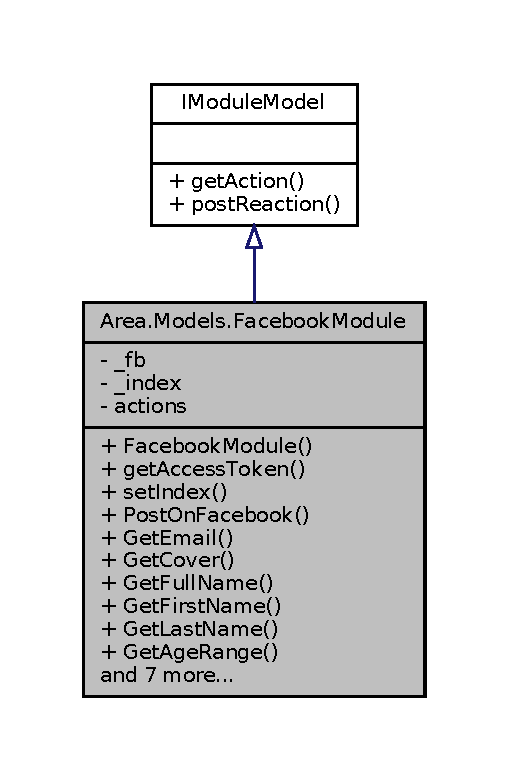
\includegraphics[width=244pt]{classArea_1_1Models_1_1FacebookModule__inherit__graph}
\end{center}
\end{figure}


Collaboration diagram for Area.\+Models.\+Facebook\+Module\+:
\nopagebreak
\begin{figure}[H]
\begin{center}
\leavevmode
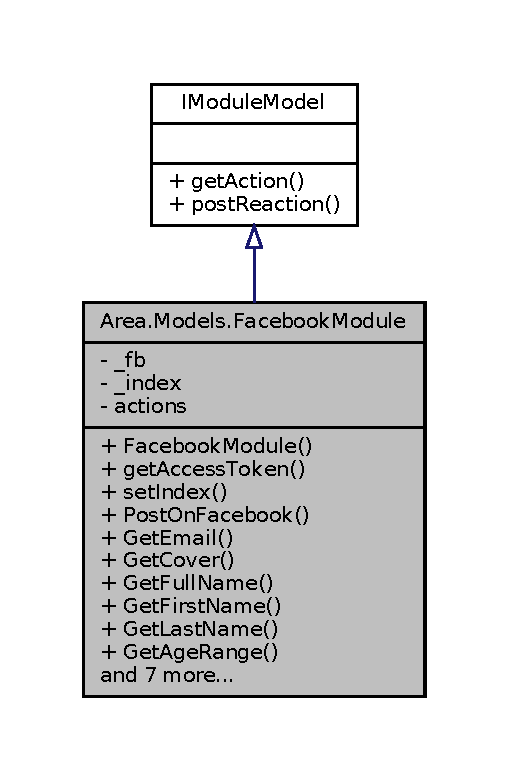
\includegraphics[width=244pt]{classArea_1_1Models_1_1FacebookModule__coll__graph}
\end{center}
\end{figure}
\subsection*{Public Member Functions}
\begin{DoxyCompactItemize}
\item 
\mbox{\hyperlink{classArea_1_1Models_1_1FacebookModule_ae316294726eb340c34653d405b244682}{Facebook\+Module}} (string access\+Token, int index)
\item 
string \mbox{\hyperlink{classArea_1_1Models_1_1FacebookModule_a2945ca6108f012ea53ea172e97bcd267}{get\+Access\+Token}} ()
\item 
void \mbox{\hyperlink{classArea_1_1Models_1_1FacebookModule_ace52541633256d5401d817e8e83a8753}{set\+Index}} (int idx)
\item 
void \mbox{\hyperlink{classArea_1_1Models_1_1FacebookModule_a374b7b02158cb5b6a128d309fe355638}{Post\+On\+Facebook}} (string to\+Post)
\item 
string \mbox{\hyperlink{classArea_1_1Models_1_1FacebookModule_a5f6a9c9d1fbbb460c4dce234cda99e5e}{Get\+Email}} ()
\item 
string \mbox{\hyperlink{classArea_1_1Models_1_1FacebookModule_a1e30037d6e0356e4600b944125f4fbe7}{Get\+Cover}} ()
\item 
string \mbox{\hyperlink{classArea_1_1Models_1_1FacebookModule_af68384d31672703c55507bf26cbb22bf}{Get\+Full\+Name}} ()
\item 
string \mbox{\hyperlink{classArea_1_1Models_1_1FacebookModule_a3684449e4150b927a132f20c52e7b568}{Get\+First\+Name}} ()
\item 
string \mbox{\hyperlink{classArea_1_1Models_1_1FacebookModule_a6a914f79bdec507a46726e8633f9e8c1}{Get\+Last\+Name}} ()
\item 
string \mbox{\hyperlink{classArea_1_1Models_1_1FacebookModule_aa43092f0d311e77e152eb60963d90de5}{Get\+Age\+Range}} ()
\item 
string \mbox{\hyperlink{classArea_1_1Models_1_1FacebookModule_ae92704bd810ff0c1aadba2e970292280}{Get\+Gender}} ()
\item 
string \mbox{\hyperlink{classArea_1_1Models_1_1FacebookModule_ab9a21a8a45ed5426a2a92e2fcdb440f4}{Get\+Locale}} ()
\item 
string \mbox{\hyperlink{classArea_1_1Models_1_1FacebookModule_a8aaaadbcc1671809ce22415b38dd2d50}{Get\+Picture}} ()
\item 
string \mbox{\hyperlink{classArea_1_1Models_1_1FacebookModule_a83085dabb1a020b586486e67f9814b76}{Get\+User\+Last\+Posts}} ()
\item 
string \mbox{\hyperlink{classArea_1_1Models_1_1FacebookModule_a86f4f25674d0aef1fc39293f40960c29}{Get\+User\+Last\+Posts\+Epured}} ()
\item 
string \mbox{\hyperlink{classArea_1_1Models_1_1FacebookModule_aeb88d4de280aa76fa80c92509b7df265}{get\+Action}} ()
\item 
void \mbox{\hyperlink{classArea_1_1Models_1_1FacebookModule_aa992d24aaa0e9ebd0a2f2c38607222d5}{post\+Reaction}} (string reaction)
\end{DoxyCompactItemize}
\subsection*{Private Attributes}
\begin{DoxyCompactItemize}
\item 
Facebook\+Client \mbox{\hyperlink{classArea_1_1Models_1_1FacebookModule_a01ca890a1b43dd2765a55e8dbe1b6708}{\+\_\+fb}} = new Facebook\+Client()
\item 
int \mbox{\hyperlink{classArea_1_1Models_1_1FacebookModule_a3c45be1580ff5b5853497647af595c36}{\+\_\+index}}
\item 
Dictionary$<$ int, Func$<$ string $>$ $>$ \mbox{\hyperlink{classArea_1_1Models_1_1FacebookModule_a6fbe12ae79bf0e6d3a4b24048c4736a6}{actions}} = new Dictionary$<$int, Func$<$string$>$$>$()
\end{DoxyCompactItemize}


\subsection{Constructor \& Destructor Documentation}
\mbox{\Hypertarget{classArea_1_1Models_1_1FacebookModule_ae316294726eb340c34653d405b244682}\label{classArea_1_1Models_1_1FacebookModule_ae316294726eb340c34653d405b244682}} 
\index{Area\+::\+Models\+::\+Facebook\+Module@{Area\+::\+Models\+::\+Facebook\+Module}!Facebook\+Module@{Facebook\+Module}}
\index{Facebook\+Module@{Facebook\+Module}!Area\+::\+Models\+::\+Facebook\+Module@{Area\+::\+Models\+::\+Facebook\+Module}}
\subsubsection{\texorpdfstring{Facebook\+Module()}{FacebookModule()}}
{\footnotesize\ttfamily Area.\+Models.\+Facebook\+Module.\+Facebook\+Module (\begin{DoxyParamCaption}\item[{string}]{access\+Token,  }\item[{int}]{index }\end{DoxyParamCaption})\hspace{0.3cm}{\ttfamily [inline]}}



\subsection{Member Function Documentation}
\mbox{\Hypertarget{classArea_1_1Models_1_1FacebookModule_a2945ca6108f012ea53ea172e97bcd267}\label{classArea_1_1Models_1_1FacebookModule_a2945ca6108f012ea53ea172e97bcd267}} 
\index{Area\+::\+Models\+::\+Facebook\+Module@{Area\+::\+Models\+::\+Facebook\+Module}!get\+Access\+Token@{get\+Access\+Token}}
\index{get\+Access\+Token@{get\+Access\+Token}!Area\+::\+Models\+::\+Facebook\+Module@{Area\+::\+Models\+::\+Facebook\+Module}}
\subsubsection{\texorpdfstring{get\+Access\+Token()}{getAccessToken()}}
{\footnotesize\ttfamily string Area.\+Models.\+Facebook\+Module.\+get\+Access\+Token (\begin{DoxyParamCaption}{ }\end{DoxyParamCaption})\hspace{0.3cm}{\ttfamily [inline]}}

\mbox{\Hypertarget{classArea_1_1Models_1_1FacebookModule_aeb88d4de280aa76fa80c92509b7df265}\label{classArea_1_1Models_1_1FacebookModule_aeb88d4de280aa76fa80c92509b7df265}} 
\index{Area\+::\+Models\+::\+Facebook\+Module@{Area\+::\+Models\+::\+Facebook\+Module}!get\+Action@{get\+Action}}
\index{get\+Action@{get\+Action}!Area\+::\+Models\+::\+Facebook\+Module@{Area\+::\+Models\+::\+Facebook\+Module}}
\subsubsection{\texorpdfstring{get\+Action()}{getAction()}}
{\footnotesize\ttfamily string Area.\+Models.\+Facebook\+Module.\+get\+Action (\begin{DoxyParamCaption}{ }\end{DoxyParamCaption})\hspace{0.3cm}{\ttfamily [inline]}}



Implements \mbox{\hyperlink{interfaceArea_1_1Models_1_1IModuleModel_a050d892fae9f85c6b607a7c0e30502e9}{Area.\+Models.\+I\+Module\+Model}}.

\mbox{\Hypertarget{classArea_1_1Models_1_1FacebookModule_aa43092f0d311e77e152eb60963d90de5}\label{classArea_1_1Models_1_1FacebookModule_aa43092f0d311e77e152eb60963d90de5}} 
\index{Area\+::\+Models\+::\+Facebook\+Module@{Area\+::\+Models\+::\+Facebook\+Module}!Get\+Age\+Range@{Get\+Age\+Range}}
\index{Get\+Age\+Range@{Get\+Age\+Range}!Area\+::\+Models\+::\+Facebook\+Module@{Area\+::\+Models\+::\+Facebook\+Module}}
\subsubsection{\texorpdfstring{Get\+Age\+Range()}{GetAgeRange()}}
{\footnotesize\ttfamily string Area.\+Models.\+Facebook\+Module.\+Get\+Age\+Range (\begin{DoxyParamCaption}{ }\end{DoxyParamCaption})\hspace{0.3cm}{\ttfamily [inline]}}

\mbox{\Hypertarget{classArea_1_1Models_1_1FacebookModule_a1e30037d6e0356e4600b944125f4fbe7}\label{classArea_1_1Models_1_1FacebookModule_a1e30037d6e0356e4600b944125f4fbe7}} 
\index{Area\+::\+Models\+::\+Facebook\+Module@{Area\+::\+Models\+::\+Facebook\+Module}!Get\+Cover@{Get\+Cover}}
\index{Get\+Cover@{Get\+Cover}!Area\+::\+Models\+::\+Facebook\+Module@{Area\+::\+Models\+::\+Facebook\+Module}}
\subsubsection{\texorpdfstring{Get\+Cover()}{GetCover()}}
{\footnotesize\ttfamily string Area.\+Models.\+Facebook\+Module.\+Get\+Cover (\begin{DoxyParamCaption}{ }\end{DoxyParamCaption})\hspace{0.3cm}{\ttfamily [inline]}}

\mbox{\Hypertarget{classArea_1_1Models_1_1FacebookModule_a5f6a9c9d1fbbb460c4dce234cda99e5e}\label{classArea_1_1Models_1_1FacebookModule_a5f6a9c9d1fbbb460c4dce234cda99e5e}} 
\index{Area\+::\+Models\+::\+Facebook\+Module@{Area\+::\+Models\+::\+Facebook\+Module}!Get\+Email@{Get\+Email}}
\index{Get\+Email@{Get\+Email}!Area\+::\+Models\+::\+Facebook\+Module@{Area\+::\+Models\+::\+Facebook\+Module}}
\subsubsection{\texorpdfstring{Get\+Email()}{GetEmail()}}
{\footnotesize\ttfamily string Area.\+Models.\+Facebook\+Module.\+Get\+Email (\begin{DoxyParamCaption}{ }\end{DoxyParamCaption})\hspace{0.3cm}{\ttfamily [inline]}}

\mbox{\Hypertarget{classArea_1_1Models_1_1FacebookModule_a3684449e4150b927a132f20c52e7b568}\label{classArea_1_1Models_1_1FacebookModule_a3684449e4150b927a132f20c52e7b568}} 
\index{Area\+::\+Models\+::\+Facebook\+Module@{Area\+::\+Models\+::\+Facebook\+Module}!Get\+First\+Name@{Get\+First\+Name}}
\index{Get\+First\+Name@{Get\+First\+Name}!Area\+::\+Models\+::\+Facebook\+Module@{Area\+::\+Models\+::\+Facebook\+Module}}
\subsubsection{\texorpdfstring{Get\+First\+Name()}{GetFirstName()}}
{\footnotesize\ttfamily string Area.\+Models.\+Facebook\+Module.\+Get\+First\+Name (\begin{DoxyParamCaption}{ }\end{DoxyParamCaption})\hspace{0.3cm}{\ttfamily [inline]}}

\mbox{\Hypertarget{classArea_1_1Models_1_1FacebookModule_af68384d31672703c55507bf26cbb22bf}\label{classArea_1_1Models_1_1FacebookModule_af68384d31672703c55507bf26cbb22bf}} 
\index{Area\+::\+Models\+::\+Facebook\+Module@{Area\+::\+Models\+::\+Facebook\+Module}!Get\+Full\+Name@{Get\+Full\+Name}}
\index{Get\+Full\+Name@{Get\+Full\+Name}!Area\+::\+Models\+::\+Facebook\+Module@{Area\+::\+Models\+::\+Facebook\+Module}}
\subsubsection{\texorpdfstring{Get\+Full\+Name()}{GetFullName()}}
{\footnotesize\ttfamily string Area.\+Models.\+Facebook\+Module.\+Get\+Full\+Name (\begin{DoxyParamCaption}{ }\end{DoxyParamCaption})\hspace{0.3cm}{\ttfamily [inline]}}

\mbox{\Hypertarget{classArea_1_1Models_1_1FacebookModule_ae92704bd810ff0c1aadba2e970292280}\label{classArea_1_1Models_1_1FacebookModule_ae92704bd810ff0c1aadba2e970292280}} 
\index{Area\+::\+Models\+::\+Facebook\+Module@{Area\+::\+Models\+::\+Facebook\+Module}!Get\+Gender@{Get\+Gender}}
\index{Get\+Gender@{Get\+Gender}!Area\+::\+Models\+::\+Facebook\+Module@{Area\+::\+Models\+::\+Facebook\+Module}}
\subsubsection{\texorpdfstring{Get\+Gender()}{GetGender()}}
{\footnotesize\ttfamily string Area.\+Models.\+Facebook\+Module.\+Get\+Gender (\begin{DoxyParamCaption}{ }\end{DoxyParamCaption})\hspace{0.3cm}{\ttfamily [inline]}}

\mbox{\Hypertarget{classArea_1_1Models_1_1FacebookModule_a6a914f79bdec507a46726e8633f9e8c1}\label{classArea_1_1Models_1_1FacebookModule_a6a914f79bdec507a46726e8633f9e8c1}} 
\index{Area\+::\+Models\+::\+Facebook\+Module@{Area\+::\+Models\+::\+Facebook\+Module}!Get\+Last\+Name@{Get\+Last\+Name}}
\index{Get\+Last\+Name@{Get\+Last\+Name}!Area\+::\+Models\+::\+Facebook\+Module@{Area\+::\+Models\+::\+Facebook\+Module}}
\subsubsection{\texorpdfstring{Get\+Last\+Name()}{GetLastName()}}
{\footnotesize\ttfamily string Area.\+Models.\+Facebook\+Module.\+Get\+Last\+Name (\begin{DoxyParamCaption}{ }\end{DoxyParamCaption})\hspace{0.3cm}{\ttfamily [inline]}}

\mbox{\Hypertarget{classArea_1_1Models_1_1FacebookModule_ab9a21a8a45ed5426a2a92e2fcdb440f4}\label{classArea_1_1Models_1_1FacebookModule_ab9a21a8a45ed5426a2a92e2fcdb440f4}} 
\index{Area\+::\+Models\+::\+Facebook\+Module@{Area\+::\+Models\+::\+Facebook\+Module}!Get\+Locale@{Get\+Locale}}
\index{Get\+Locale@{Get\+Locale}!Area\+::\+Models\+::\+Facebook\+Module@{Area\+::\+Models\+::\+Facebook\+Module}}
\subsubsection{\texorpdfstring{Get\+Locale()}{GetLocale()}}
{\footnotesize\ttfamily string Area.\+Models.\+Facebook\+Module.\+Get\+Locale (\begin{DoxyParamCaption}{ }\end{DoxyParamCaption})\hspace{0.3cm}{\ttfamily [inline]}}

\mbox{\Hypertarget{classArea_1_1Models_1_1FacebookModule_a8aaaadbcc1671809ce22415b38dd2d50}\label{classArea_1_1Models_1_1FacebookModule_a8aaaadbcc1671809ce22415b38dd2d50}} 
\index{Area\+::\+Models\+::\+Facebook\+Module@{Area\+::\+Models\+::\+Facebook\+Module}!Get\+Picture@{Get\+Picture}}
\index{Get\+Picture@{Get\+Picture}!Area\+::\+Models\+::\+Facebook\+Module@{Area\+::\+Models\+::\+Facebook\+Module}}
\subsubsection{\texorpdfstring{Get\+Picture()}{GetPicture()}}
{\footnotesize\ttfamily string Area.\+Models.\+Facebook\+Module.\+Get\+Picture (\begin{DoxyParamCaption}{ }\end{DoxyParamCaption})\hspace{0.3cm}{\ttfamily [inline]}}

\mbox{\Hypertarget{classArea_1_1Models_1_1FacebookModule_a83085dabb1a020b586486e67f9814b76}\label{classArea_1_1Models_1_1FacebookModule_a83085dabb1a020b586486e67f9814b76}} 
\index{Area\+::\+Models\+::\+Facebook\+Module@{Area\+::\+Models\+::\+Facebook\+Module}!Get\+User\+Last\+Posts@{Get\+User\+Last\+Posts}}
\index{Get\+User\+Last\+Posts@{Get\+User\+Last\+Posts}!Area\+::\+Models\+::\+Facebook\+Module@{Area\+::\+Models\+::\+Facebook\+Module}}
\subsubsection{\texorpdfstring{Get\+User\+Last\+Posts()}{GetUserLastPosts()}}
{\footnotesize\ttfamily string Area.\+Models.\+Facebook\+Module.\+Get\+User\+Last\+Posts (\begin{DoxyParamCaption}{ }\end{DoxyParamCaption})\hspace{0.3cm}{\ttfamily [inline]}}

\mbox{\Hypertarget{classArea_1_1Models_1_1FacebookModule_a86f4f25674d0aef1fc39293f40960c29}\label{classArea_1_1Models_1_1FacebookModule_a86f4f25674d0aef1fc39293f40960c29}} 
\index{Area\+::\+Models\+::\+Facebook\+Module@{Area\+::\+Models\+::\+Facebook\+Module}!Get\+User\+Last\+Posts\+Epured@{Get\+User\+Last\+Posts\+Epured}}
\index{Get\+User\+Last\+Posts\+Epured@{Get\+User\+Last\+Posts\+Epured}!Area\+::\+Models\+::\+Facebook\+Module@{Area\+::\+Models\+::\+Facebook\+Module}}
\subsubsection{\texorpdfstring{Get\+User\+Last\+Posts\+Epured()}{GetUserLastPostsEpured()}}
{\footnotesize\ttfamily string Area.\+Models.\+Facebook\+Module.\+Get\+User\+Last\+Posts\+Epured (\begin{DoxyParamCaption}{ }\end{DoxyParamCaption})\hspace{0.3cm}{\ttfamily [inline]}}

\mbox{\Hypertarget{classArea_1_1Models_1_1FacebookModule_a374b7b02158cb5b6a128d309fe355638}\label{classArea_1_1Models_1_1FacebookModule_a374b7b02158cb5b6a128d309fe355638}} 
\index{Area\+::\+Models\+::\+Facebook\+Module@{Area\+::\+Models\+::\+Facebook\+Module}!Post\+On\+Facebook@{Post\+On\+Facebook}}
\index{Post\+On\+Facebook@{Post\+On\+Facebook}!Area\+::\+Models\+::\+Facebook\+Module@{Area\+::\+Models\+::\+Facebook\+Module}}
\subsubsection{\texorpdfstring{Post\+On\+Facebook()}{PostOnFacebook()}}
{\footnotesize\ttfamily void Area.\+Models.\+Facebook\+Module.\+Post\+On\+Facebook (\begin{DoxyParamCaption}\item[{string}]{to\+Post }\end{DoxyParamCaption})\hspace{0.3cm}{\ttfamily [inline]}}

\mbox{\Hypertarget{classArea_1_1Models_1_1FacebookModule_aa992d24aaa0e9ebd0a2f2c38607222d5}\label{classArea_1_1Models_1_1FacebookModule_aa992d24aaa0e9ebd0a2f2c38607222d5}} 
\index{Area\+::\+Models\+::\+Facebook\+Module@{Area\+::\+Models\+::\+Facebook\+Module}!post\+Reaction@{post\+Reaction}}
\index{post\+Reaction@{post\+Reaction}!Area\+::\+Models\+::\+Facebook\+Module@{Area\+::\+Models\+::\+Facebook\+Module}}
\subsubsection{\texorpdfstring{post\+Reaction()}{postReaction()}}
{\footnotesize\ttfamily void Area.\+Models.\+Facebook\+Module.\+post\+Reaction (\begin{DoxyParamCaption}\item[{string}]{reaction }\end{DoxyParamCaption})\hspace{0.3cm}{\ttfamily [inline]}}



Implements \mbox{\hyperlink{interfaceArea_1_1Models_1_1IModuleModel_af2c1a82bd894255ab2099440f4f3d6f7}{Area.\+Models.\+I\+Module\+Model}}.

\mbox{\Hypertarget{classArea_1_1Models_1_1FacebookModule_ace52541633256d5401d817e8e83a8753}\label{classArea_1_1Models_1_1FacebookModule_ace52541633256d5401d817e8e83a8753}} 
\index{Area\+::\+Models\+::\+Facebook\+Module@{Area\+::\+Models\+::\+Facebook\+Module}!set\+Index@{set\+Index}}
\index{set\+Index@{set\+Index}!Area\+::\+Models\+::\+Facebook\+Module@{Area\+::\+Models\+::\+Facebook\+Module}}
\subsubsection{\texorpdfstring{set\+Index()}{setIndex()}}
{\footnotesize\ttfamily void Area.\+Models.\+Facebook\+Module.\+set\+Index (\begin{DoxyParamCaption}\item[{int}]{idx }\end{DoxyParamCaption})\hspace{0.3cm}{\ttfamily [inline]}}



\subsection{Member Data Documentation}
\mbox{\Hypertarget{classArea_1_1Models_1_1FacebookModule_a01ca890a1b43dd2765a55e8dbe1b6708}\label{classArea_1_1Models_1_1FacebookModule_a01ca890a1b43dd2765a55e8dbe1b6708}} 
\index{Area\+::\+Models\+::\+Facebook\+Module@{Area\+::\+Models\+::\+Facebook\+Module}!\+\_\+fb@{\+\_\+fb}}
\index{\+\_\+fb@{\+\_\+fb}!Area\+::\+Models\+::\+Facebook\+Module@{Area\+::\+Models\+::\+Facebook\+Module}}
\subsubsection{\texorpdfstring{\+\_\+fb}{\_fb}}
{\footnotesize\ttfamily Facebook\+Client Area.\+Models.\+Facebook\+Module.\+\_\+fb = new Facebook\+Client()\hspace{0.3cm}{\ttfamily [private]}}

\mbox{\Hypertarget{classArea_1_1Models_1_1FacebookModule_a3c45be1580ff5b5853497647af595c36}\label{classArea_1_1Models_1_1FacebookModule_a3c45be1580ff5b5853497647af595c36}} 
\index{Area\+::\+Models\+::\+Facebook\+Module@{Area\+::\+Models\+::\+Facebook\+Module}!\+\_\+index@{\+\_\+index}}
\index{\+\_\+index@{\+\_\+index}!Area\+::\+Models\+::\+Facebook\+Module@{Area\+::\+Models\+::\+Facebook\+Module}}
\subsubsection{\texorpdfstring{\+\_\+index}{\_index}}
{\footnotesize\ttfamily int Area.\+Models.\+Facebook\+Module.\+\_\+index\hspace{0.3cm}{\ttfamily [private]}}

\mbox{\Hypertarget{classArea_1_1Models_1_1FacebookModule_a6fbe12ae79bf0e6d3a4b24048c4736a6}\label{classArea_1_1Models_1_1FacebookModule_a6fbe12ae79bf0e6d3a4b24048c4736a6}} 
\index{Area\+::\+Models\+::\+Facebook\+Module@{Area\+::\+Models\+::\+Facebook\+Module}!actions@{actions}}
\index{actions@{actions}!Area\+::\+Models\+::\+Facebook\+Module@{Area\+::\+Models\+::\+Facebook\+Module}}
\subsubsection{\texorpdfstring{actions}{actions}}
{\footnotesize\ttfamily Dictionary$<$int, Func$<$string$>$ $>$ Area.\+Models.\+Facebook\+Module.\+actions = new Dictionary$<$int, Func$<$string$>$$>$()\hspace{0.3cm}{\ttfamily [private]}}



The documentation for this class was generated from the following file\+:\begin{DoxyCompactItemize}
\item 
Models/\+Modules/\mbox{\hyperlink{FacebookModule_8cs}{Facebook\+Module.\+cs}}\end{DoxyCompactItemize}

\hypertarget{classArea_1_1Models_1_1FacebookSpotifyArea}{}\section{Area.\+Models.\+Facebook\+Spotify\+Area Class Reference}
\label{classArea_1_1Models_1_1FacebookSpotifyArea}\index{Area.\+Models.\+Facebook\+Spotify\+Area@{Area.\+Models.\+Facebook\+Spotify\+Area}}


Inheritance diagram for Area.\+Models.\+Facebook\+Spotify\+Area\+:
\nopagebreak
\begin{figure}[H]
\begin{center}
\leavevmode
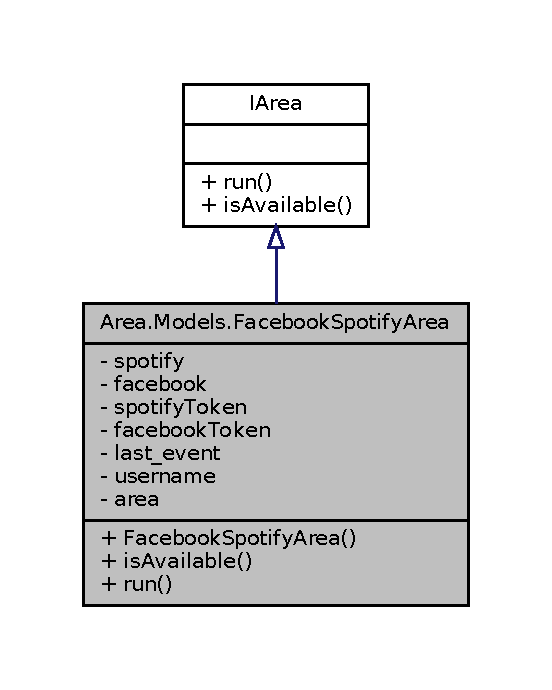
\includegraphics[width=265pt]{classArea_1_1Models_1_1FacebookSpotifyArea__inherit__graph}
\end{center}
\end{figure}


Collaboration diagram for Area.\+Models.\+Facebook\+Spotify\+Area\+:
\nopagebreak
\begin{figure}[H]
\begin{center}
\leavevmode
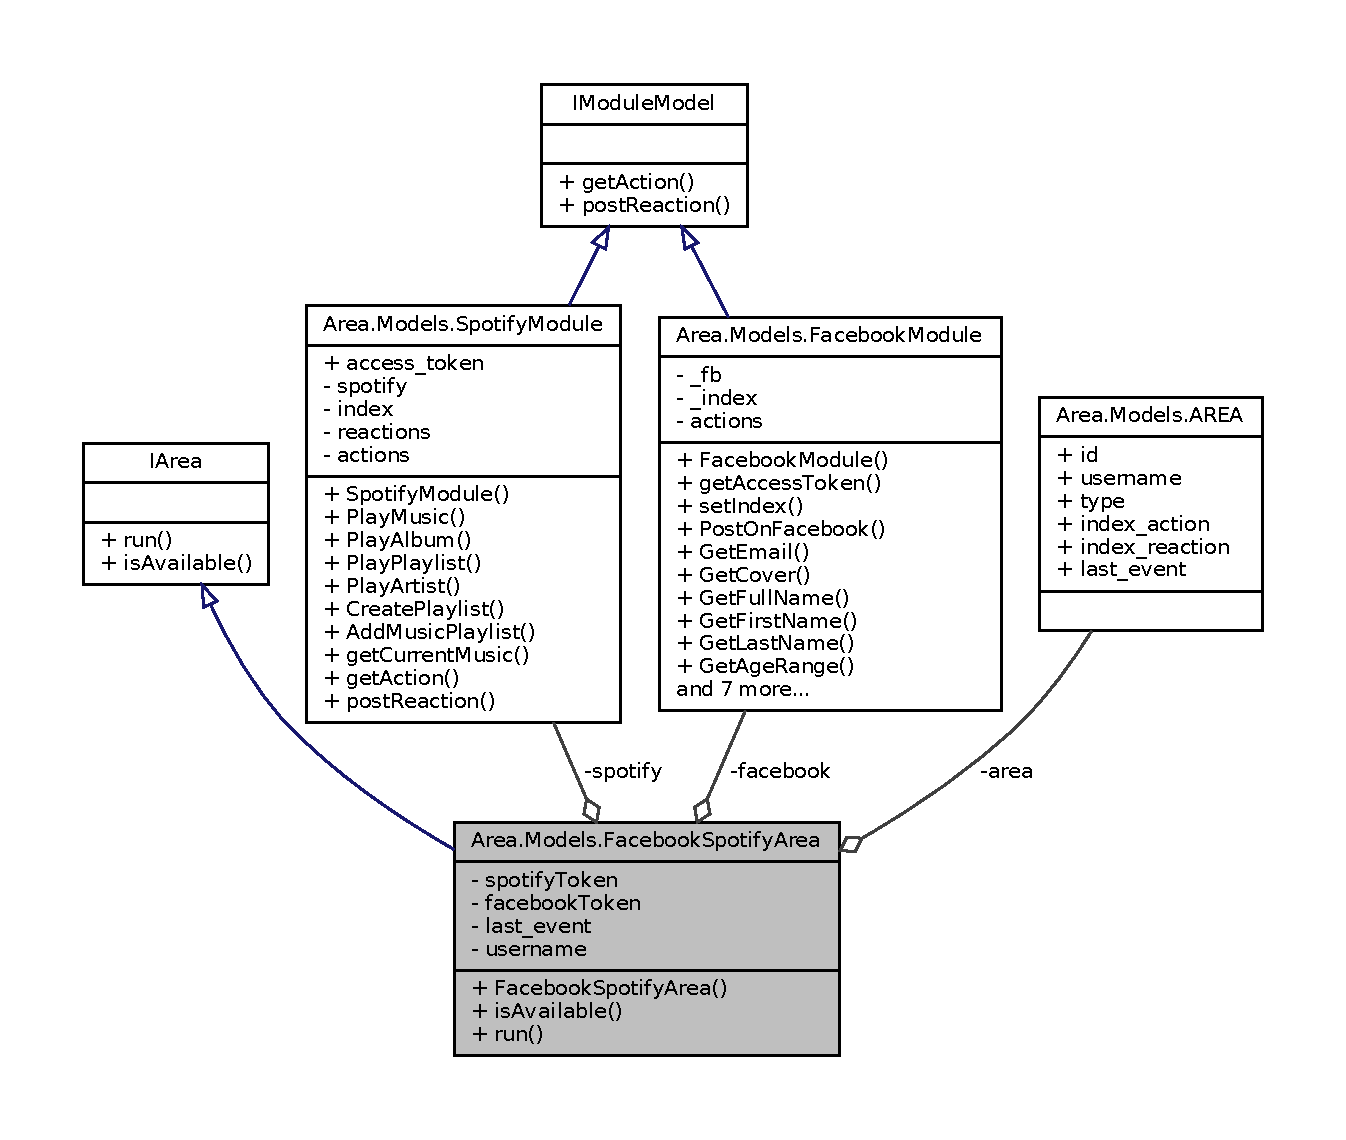
\includegraphics[width=350pt]{classArea_1_1Models_1_1FacebookSpotifyArea__coll__graph}
\end{center}
\end{figure}
\subsection*{Public Member Functions}
\begin{DoxyCompactItemize}
\item 
\mbox{\hyperlink{classArea_1_1Models_1_1FacebookSpotifyArea_af15433bc9d994b358ac7d6a4cce9c836}{Facebook\+Spotify\+Area}} (\mbox{\hyperlink{classArea_1_1Models_1_1AREA}{A\+R\+EA}} \mbox{\hyperlink{classArea_1_1Models_1_1FacebookSpotifyArea_abc59a0966bbec21ee29cf0214535542c}{area}}, \mbox{\hyperlink{classArea_1_1DAT_1_1AreaDbContext}{Area\+Db\+Context}} DB)
\item 
bool \mbox{\hyperlink{classArea_1_1Models_1_1FacebookSpotifyArea_aa98a5f78b4814107265c952496c50fcb}{is\+Available}} ()
\item 
void \mbox{\hyperlink{classArea_1_1Models_1_1FacebookSpotifyArea_ae574aa239311b4fc84d087adef335f3d}{run}} (\mbox{\hyperlink{classArea_1_1DAT_1_1AreaDbContext}{Area\+Db\+Context}} DB)
\end{DoxyCompactItemize}
\subsection*{Private Attributes}
\begin{DoxyCompactItemize}
\item 
\mbox{\hyperlink{classArea_1_1Models_1_1SpotifyModule}{Spotify\+Module}} \mbox{\hyperlink{classArea_1_1Models_1_1FacebookSpotifyArea_a8b986deb612a12826ccc6625f9f774a9}{spotify}}
\item 
\mbox{\hyperlink{classArea_1_1Models_1_1FacebookModule}{Facebook\+Module}} \mbox{\hyperlink{classArea_1_1Models_1_1FacebookSpotifyArea_a4bae14b0fd3befbc256ecf7bd557261d}{facebook}}
\item 
string \mbox{\hyperlink{classArea_1_1Models_1_1FacebookSpotifyArea_a4d5cd25335bcdabce156cfb4b479d70e}{spotify\+Token}} = \char`\"{}\char`\"{}
\item 
string \mbox{\hyperlink{classArea_1_1Models_1_1FacebookSpotifyArea_a0eed9b6d58dcb07a6c704884d12a0d6c}{facebook\+Token}} = \char`\"{}\char`\"{}
\item 
string \mbox{\hyperlink{classArea_1_1Models_1_1FacebookSpotifyArea_af4891cb5643274f6d5b05fd72248e5be}{last\+\_\+event}}
\item 
string \mbox{\hyperlink{classArea_1_1Models_1_1FacebookSpotifyArea_a50cb6f7d6d1d44a1c5ddd5997597fcab}{username}}
\item 
\mbox{\hyperlink{classArea_1_1Models_1_1AREA}{A\+R\+EA}} \mbox{\hyperlink{classArea_1_1Models_1_1FacebookSpotifyArea_abc59a0966bbec21ee29cf0214535542c}{area}}
\end{DoxyCompactItemize}


\subsection{Constructor \& Destructor Documentation}
\mbox{\Hypertarget{classArea_1_1Models_1_1FacebookSpotifyArea_af15433bc9d994b358ac7d6a4cce9c836}\label{classArea_1_1Models_1_1FacebookSpotifyArea_af15433bc9d994b358ac7d6a4cce9c836}} 
\index{Area\+::\+Models\+::\+Facebook\+Spotify\+Area@{Area\+::\+Models\+::\+Facebook\+Spotify\+Area}!Facebook\+Spotify\+Area@{Facebook\+Spotify\+Area}}
\index{Facebook\+Spotify\+Area@{Facebook\+Spotify\+Area}!Area\+::\+Models\+::\+Facebook\+Spotify\+Area@{Area\+::\+Models\+::\+Facebook\+Spotify\+Area}}
\subsubsection{\texorpdfstring{Facebook\+Spotify\+Area()}{FacebookSpotifyArea()}}
{\footnotesize\ttfamily Area.\+Models.\+Facebook\+Spotify\+Area.\+Facebook\+Spotify\+Area (\begin{DoxyParamCaption}\item[{\mbox{\hyperlink{classArea_1_1Models_1_1AREA}{A\+R\+EA}}}]{area,  }\item[{\mbox{\hyperlink{classArea_1_1DAT_1_1AreaDbContext}{Area\+Db\+Context}}}]{DB }\end{DoxyParamCaption})\hspace{0.3cm}{\ttfamily [inline]}}



\subsection{Member Function Documentation}
\mbox{\Hypertarget{classArea_1_1Models_1_1FacebookSpotifyArea_aa98a5f78b4814107265c952496c50fcb}\label{classArea_1_1Models_1_1FacebookSpotifyArea_aa98a5f78b4814107265c952496c50fcb}} 
\index{Area\+::\+Models\+::\+Facebook\+Spotify\+Area@{Area\+::\+Models\+::\+Facebook\+Spotify\+Area}!is\+Available@{is\+Available}}
\index{is\+Available@{is\+Available}!Area\+::\+Models\+::\+Facebook\+Spotify\+Area@{Area\+::\+Models\+::\+Facebook\+Spotify\+Area}}
\subsubsection{\texorpdfstring{is\+Available()}{isAvailable()}}
{\footnotesize\ttfamily bool Area.\+Models.\+Facebook\+Spotify\+Area.\+is\+Available (\begin{DoxyParamCaption}{ }\end{DoxyParamCaption})\hspace{0.3cm}{\ttfamily [inline]}}



Implements \mbox{\hyperlink{interfaceArea_1_1Models_1_1IArea_a742b324f0d7573f7f99f9e2adb5df94c}{Area.\+Models.\+I\+Area}}.

Here is the call graph for this function\+:
\nopagebreak
\begin{figure}[H]
\begin{center}
\leavevmode
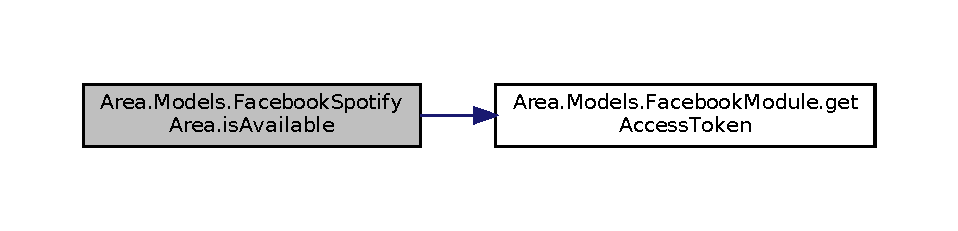
\includegraphics[width=350pt]{classArea_1_1Models_1_1FacebookSpotifyArea_aa98a5f78b4814107265c952496c50fcb_cgraph}
\end{center}
\end{figure}
\mbox{\Hypertarget{classArea_1_1Models_1_1FacebookSpotifyArea_ae574aa239311b4fc84d087adef335f3d}\label{classArea_1_1Models_1_1FacebookSpotifyArea_ae574aa239311b4fc84d087adef335f3d}} 
\index{Area\+::\+Models\+::\+Facebook\+Spotify\+Area@{Area\+::\+Models\+::\+Facebook\+Spotify\+Area}!run@{run}}
\index{run@{run}!Area\+::\+Models\+::\+Facebook\+Spotify\+Area@{Area\+::\+Models\+::\+Facebook\+Spotify\+Area}}
\subsubsection{\texorpdfstring{run()}{run()}}
{\footnotesize\ttfamily void Area.\+Models.\+Facebook\+Spotify\+Area.\+run (\begin{DoxyParamCaption}\item[{\mbox{\hyperlink{classArea_1_1DAT_1_1AreaDbContext}{Area\+Db\+Context}}}]{DB }\end{DoxyParamCaption})\hspace{0.3cm}{\ttfamily [inline]}}



Implements \mbox{\hyperlink{interfaceArea_1_1Models_1_1IArea_af153822d2715dad8eb1c250bcc4de567}{Area.\+Models.\+I\+Area}}.

Here is the call graph for this function\+:
\nopagebreak
\begin{figure}[H]
\begin{center}
\leavevmode
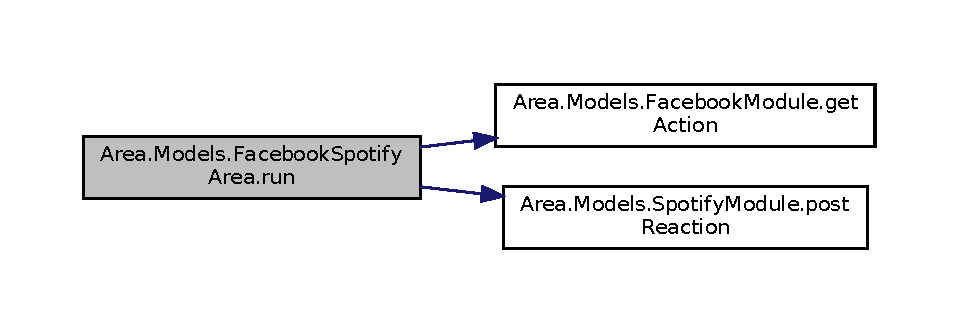
\includegraphics[width=350pt]{classArea_1_1Models_1_1FacebookSpotifyArea_ae574aa239311b4fc84d087adef335f3d_cgraph}
\end{center}
\end{figure}


\subsection{Member Data Documentation}
\mbox{\Hypertarget{classArea_1_1Models_1_1FacebookSpotifyArea_abc59a0966bbec21ee29cf0214535542c}\label{classArea_1_1Models_1_1FacebookSpotifyArea_abc59a0966bbec21ee29cf0214535542c}} 
\index{Area\+::\+Models\+::\+Facebook\+Spotify\+Area@{Area\+::\+Models\+::\+Facebook\+Spotify\+Area}!area@{area}}
\index{area@{area}!Area\+::\+Models\+::\+Facebook\+Spotify\+Area@{Area\+::\+Models\+::\+Facebook\+Spotify\+Area}}
\subsubsection{\texorpdfstring{area}{area}}
{\footnotesize\ttfamily \mbox{\hyperlink{classArea_1_1Models_1_1AREA}{A\+R\+EA}} Area.\+Models.\+Facebook\+Spotify\+Area.\+area\hspace{0.3cm}{\ttfamily [private]}}

\mbox{\Hypertarget{classArea_1_1Models_1_1FacebookSpotifyArea_a4bae14b0fd3befbc256ecf7bd557261d}\label{classArea_1_1Models_1_1FacebookSpotifyArea_a4bae14b0fd3befbc256ecf7bd557261d}} 
\index{Area\+::\+Models\+::\+Facebook\+Spotify\+Area@{Area\+::\+Models\+::\+Facebook\+Spotify\+Area}!facebook@{facebook}}
\index{facebook@{facebook}!Area\+::\+Models\+::\+Facebook\+Spotify\+Area@{Area\+::\+Models\+::\+Facebook\+Spotify\+Area}}
\subsubsection{\texorpdfstring{facebook}{facebook}}
{\footnotesize\ttfamily \mbox{\hyperlink{classArea_1_1Models_1_1FacebookModule}{Facebook\+Module}} Area.\+Models.\+Facebook\+Spotify\+Area.\+facebook\hspace{0.3cm}{\ttfamily [private]}}

\mbox{\Hypertarget{classArea_1_1Models_1_1FacebookSpotifyArea_a0eed9b6d58dcb07a6c704884d12a0d6c}\label{classArea_1_1Models_1_1FacebookSpotifyArea_a0eed9b6d58dcb07a6c704884d12a0d6c}} 
\index{Area\+::\+Models\+::\+Facebook\+Spotify\+Area@{Area\+::\+Models\+::\+Facebook\+Spotify\+Area}!facebook\+Token@{facebook\+Token}}
\index{facebook\+Token@{facebook\+Token}!Area\+::\+Models\+::\+Facebook\+Spotify\+Area@{Area\+::\+Models\+::\+Facebook\+Spotify\+Area}}
\subsubsection{\texorpdfstring{facebook\+Token}{facebookToken}}
{\footnotesize\ttfamily string Area.\+Models.\+Facebook\+Spotify\+Area.\+facebook\+Token = \char`\"{}\char`\"{}\hspace{0.3cm}{\ttfamily [private]}}

\mbox{\Hypertarget{classArea_1_1Models_1_1FacebookSpotifyArea_af4891cb5643274f6d5b05fd72248e5be}\label{classArea_1_1Models_1_1FacebookSpotifyArea_af4891cb5643274f6d5b05fd72248e5be}} 
\index{Area\+::\+Models\+::\+Facebook\+Spotify\+Area@{Area\+::\+Models\+::\+Facebook\+Spotify\+Area}!last\+\_\+event@{last\+\_\+event}}
\index{last\+\_\+event@{last\+\_\+event}!Area\+::\+Models\+::\+Facebook\+Spotify\+Area@{Area\+::\+Models\+::\+Facebook\+Spotify\+Area}}
\subsubsection{\texorpdfstring{last\+\_\+event}{last\_event}}
{\footnotesize\ttfamily string Area.\+Models.\+Facebook\+Spotify\+Area.\+last\+\_\+event\hspace{0.3cm}{\ttfamily [private]}}

\mbox{\Hypertarget{classArea_1_1Models_1_1FacebookSpotifyArea_a8b986deb612a12826ccc6625f9f774a9}\label{classArea_1_1Models_1_1FacebookSpotifyArea_a8b986deb612a12826ccc6625f9f774a9}} 
\index{Area\+::\+Models\+::\+Facebook\+Spotify\+Area@{Area\+::\+Models\+::\+Facebook\+Spotify\+Area}!spotify@{spotify}}
\index{spotify@{spotify}!Area\+::\+Models\+::\+Facebook\+Spotify\+Area@{Area\+::\+Models\+::\+Facebook\+Spotify\+Area}}
\subsubsection{\texorpdfstring{spotify}{spotify}}
{\footnotesize\ttfamily \mbox{\hyperlink{classArea_1_1Models_1_1SpotifyModule}{Spotify\+Module}} Area.\+Models.\+Facebook\+Spotify\+Area.\+spotify\hspace{0.3cm}{\ttfamily [private]}}

\mbox{\Hypertarget{classArea_1_1Models_1_1FacebookSpotifyArea_a4d5cd25335bcdabce156cfb4b479d70e}\label{classArea_1_1Models_1_1FacebookSpotifyArea_a4d5cd25335bcdabce156cfb4b479d70e}} 
\index{Area\+::\+Models\+::\+Facebook\+Spotify\+Area@{Area\+::\+Models\+::\+Facebook\+Spotify\+Area}!spotify\+Token@{spotify\+Token}}
\index{spotify\+Token@{spotify\+Token}!Area\+::\+Models\+::\+Facebook\+Spotify\+Area@{Area\+::\+Models\+::\+Facebook\+Spotify\+Area}}
\subsubsection{\texorpdfstring{spotify\+Token}{spotifyToken}}
{\footnotesize\ttfamily string Area.\+Models.\+Facebook\+Spotify\+Area.\+spotify\+Token = \char`\"{}\char`\"{}\hspace{0.3cm}{\ttfamily [private]}}

\mbox{\Hypertarget{classArea_1_1Models_1_1FacebookSpotifyArea_a50cb6f7d6d1d44a1c5ddd5997597fcab}\label{classArea_1_1Models_1_1FacebookSpotifyArea_a50cb6f7d6d1d44a1c5ddd5997597fcab}} 
\index{Area\+::\+Models\+::\+Facebook\+Spotify\+Area@{Area\+::\+Models\+::\+Facebook\+Spotify\+Area}!username@{username}}
\index{username@{username}!Area\+::\+Models\+::\+Facebook\+Spotify\+Area@{Area\+::\+Models\+::\+Facebook\+Spotify\+Area}}
\subsubsection{\texorpdfstring{username}{username}}
{\footnotesize\ttfamily string Area.\+Models.\+Facebook\+Spotify\+Area.\+username\hspace{0.3cm}{\ttfamily [private]}}



The documentation for this class was generated from the following file\+:\begin{DoxyCompactItemize}
\item 
Models/\+Areas/\mbox{\hyperlink{FacebookSpotifyArea_8cs}{Facebook\+Spotify\+Area.\+cs}}\end{DoxyCompactItemize}

\hypertarget{classArea_1_1Controllers_1_1FacebookSpotifyAreaController}{}\section{Area.\+Controllers.\+Facebook\+Spotify\+Area\+Controller Class Reference}
\label{classArea_1_1Controllers_1_1FacebookSpotifyAreaController}\index{Area.\+Controllers.\+Facebook\+Spotify\+Area\+Controller@{Area.\+Controllers.\+Facebook\+Spotify\+Area\+Controller}}


Inheritance diagram for Area.\+Controllers.\+Facebook\+Spotify\+Area\+Controller\+:
\nopagebreak
\begin{figure}[H]
\begin{center}
\leavevmode
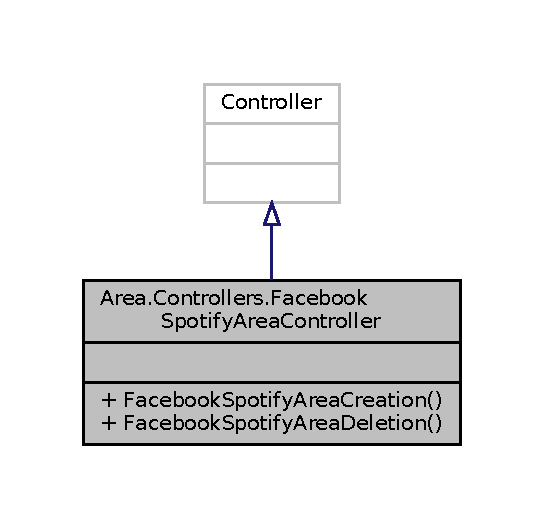
\includegraphics[width=261pt]{classArea_1_1Controllers_1_1FacebookSpotifyAreaController__inherit__graph}
\end{center}
\end{figure}


Collaboration diagram for Area.\+Controllers.\+Facebook\+Spotify\+Area\+Controller\+:
\nopagebreak
\begin{figure}[H]
\begin{center}
\leavevmode
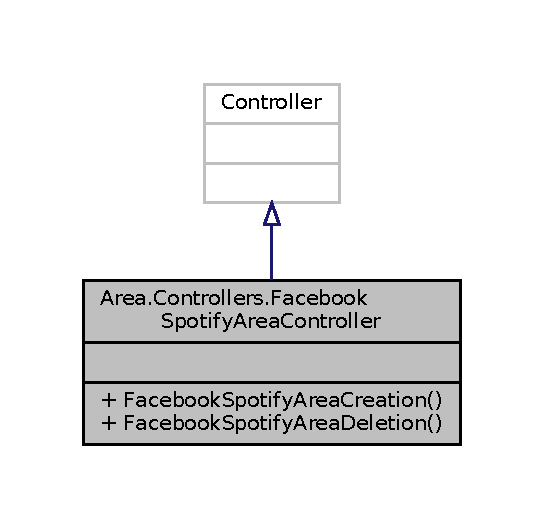
\includegraphics[width=261pt]{classArea_1_1Controllers_1_1FacebookSpotifyAreaController__coll__graph}
\end{center}
\end{figure}
\subsection*{Public Member Functions}
\begin{DoxyCompactItemize}
\item 
Action\+Result \mbox{\hyperlink{classArea_1_1Controllers_1_1FacebookSpotifyAreaController_a7e7859f0e88380c50e0486e25344c822}{Facebook\+Spotify\+Area\+Creation}} (string action\+\_\+index, string reaction\+\_\+index, \mbox{[}From\+Services\mbox{]} \mbox{\hyperlink{classArea_1_1DAT_1_1AreaDbContext}{Area\+Db\+Context}} DB)
\item 
Action\+Result \mbox{\hyperlink{classArea_1_1Controllers_1_1FacebookSpotifyAreaController_ad03e220743db8b630b3f36e9f3e5dfcd}{Facebook\+Spotify\+Area\+Deletion}} (string action\+\_\+index, string reaction\+\_\+index, \mbox{[}From\+Services\mbox{]} \mbox{\hyperlink{classArea_1_1DAT_1_1AreaDbContext}{Area\+Db\+Context}} DB)
\end{DoxyCompactItemize}


\subsection{Member Function Documentation}
\mbox{\Hypertarget{classArea_1_1Controllers_1_1FacebookSpotifyAreaController_a7e7859f0e88380c50e0486e25344c822}\label{classArea_1_1Controllers_1_1FacebookSpotifyAreaController_a7e7859f0e88380c50e0486e25344c822}} 
\index{Area\+::\+Controllers\+::\+Facebook\+Spotify\+Area\+Controller@{Area\+::\+Controllers\+::\+Facebook\+Spotify\+Area\+Controller}!Facebook\+Spotify\+Area\+Creation@{Facebook\+Spotify\+Area\+Creation}}
\index{Facebook\+Spotify\+Area\+Creation@{Facebook\+Spotify\+Area\+Creation}!Area\+::\+Controllers\+::\+Facebook\+Spotify\+Area\+Controller@{Area\+::\+Controllers\+::\+Facebook\+Spotify\+Area\+Controller}}
\subsubsection{\texorpdfstring{Facebook\+Spotify\+Area\+Creation()}{FacebookSpotifyAreaCreation()}}
{\footnotesize\ttfamily Action\+Result Area.\+Controllers.\+Facebook\+Spotify\+Area\+Controller.\+Facebook\+Spotify\+Area\+Creation (\begin{DoxyParamCaption}\item[{string}]{action\+\_\+index,  }\item[{string}]{reaction\+\_\+index,  }\item[{\mbox{[}\+From\+Services\mbox{]} \mbox{\hyperlink{classArea_1_1DAT_1_1AreaDbContext}{Area\+Db\+Context}}}]{DB }\end{DoxyParamCaption})\hspace{0.3cm}{\ttfamily [inline]}}

\mbox{\Hypertarget{classArea_1_1Controllers_1_1FacebookSpotifyAreaController_ad03e220743db8b630b3f36e9f3e5dfcd}\label{classArea_1_1Controllers_1_1FacebookSpotifyAreaController_ad03e220743db8b630b3f36e9f3e5dfcd}} 
\index{Area\+::\+Controllers\+::\+Facebook\+Spotify\+Area\+Controller@{Area\+::\+Controllers\+::\+Facebook\+Spotify\+Area\+Controller}!Facebook\+Spotify\+Area\+Deletion@{Facebook\+Spotify\+Area\+Deletion}}
\index{Facebook\+Spotify\+Area\+Deletion@{Facebook\+Spotify\+Area\+Deletion}!Area\+::\+Controllers\+::\+Facebook\+Spotify\+Area\+Controller@{Area\+::\+Controllers\+::\+Facebook\+Spotify\+Area\+Controller}}
\subsubsection{\texorpdfstring{Facebook\+Spotify\+Area\+Deletion()}{FacebookSpotifyAreaDeletion()}}
{\footnotesize\ttfamily Action\+Result Area.\+Controllers.\+Facebook\+Spotify\+Area\+Controller.\+Facebook\+Spotify\+Area\+Deletion (\begin{DoxyParamCaption}\item[{string}]{action\+\_\+index,  }\item[{string}]{reaction\+\_\+index,  }\item[{\mbox{[}\+From\+Services\mbox{]} \mbox{\hyperlink{classArea_1_1DAT_1_1AreaDbContext}{Area\+Db\+Context}}}]{DB }\end{DoxyParamCaption})\hspace{0.3cm}{\ttfamily [inline]}}



The documentation for this class was generated from the following file\+:\begin{DoxyCompactItemize}
\item 
Controllers/\mbox{\hyperlink{FacebookSpotifyAreaController_8cs}{Facebook\+Spotify\+Area\+Controller.\+cs}}\end{DoxyCompactItemize}

\hypertarget{classArea_1_1Models_1_1FacebookTwitterArea}{}\section{Area.\+Models.\+Facebook\+Twitter\+Area Class Reference}
\label{classArea_1_1Models_1_1FacebookTwitterArea}\index{Area.\+Models.\+Facebook\+Twitter\+Area@{Area.\+Models.\+Facebook\+Twitter\+Area}}


Inheritance diagram for Area.\+Models.\+Facebook\+Twitter\+Area\+:
\nopagebreak
\begin{figure}[H]
\begin{center}
\leavevmode
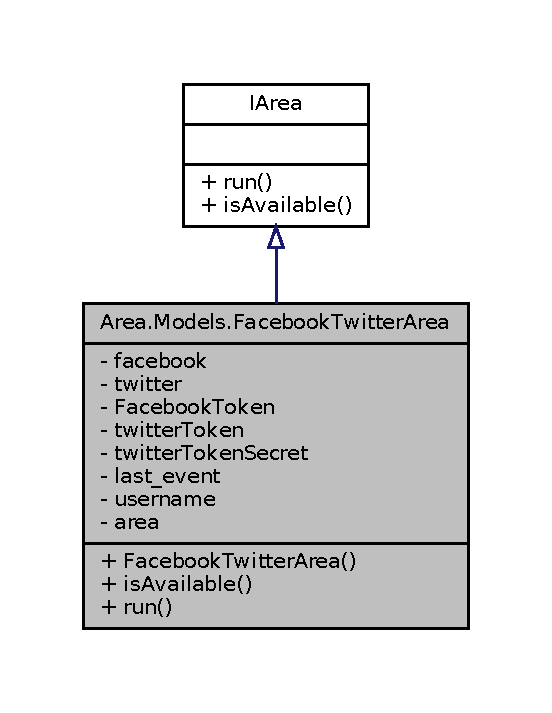
\includegraphics[width=265pt]{classArea_1_1Models_1_1FacebookTwitterArea__inherit__graph}
\end{center}
\end{figure}


Collaboration diagram for Area.\+Models.\+Facebook\+Twitter\+Area\+:
\nopagebreak
\begin{figure}[H]
\begin{center}
\leavevmode
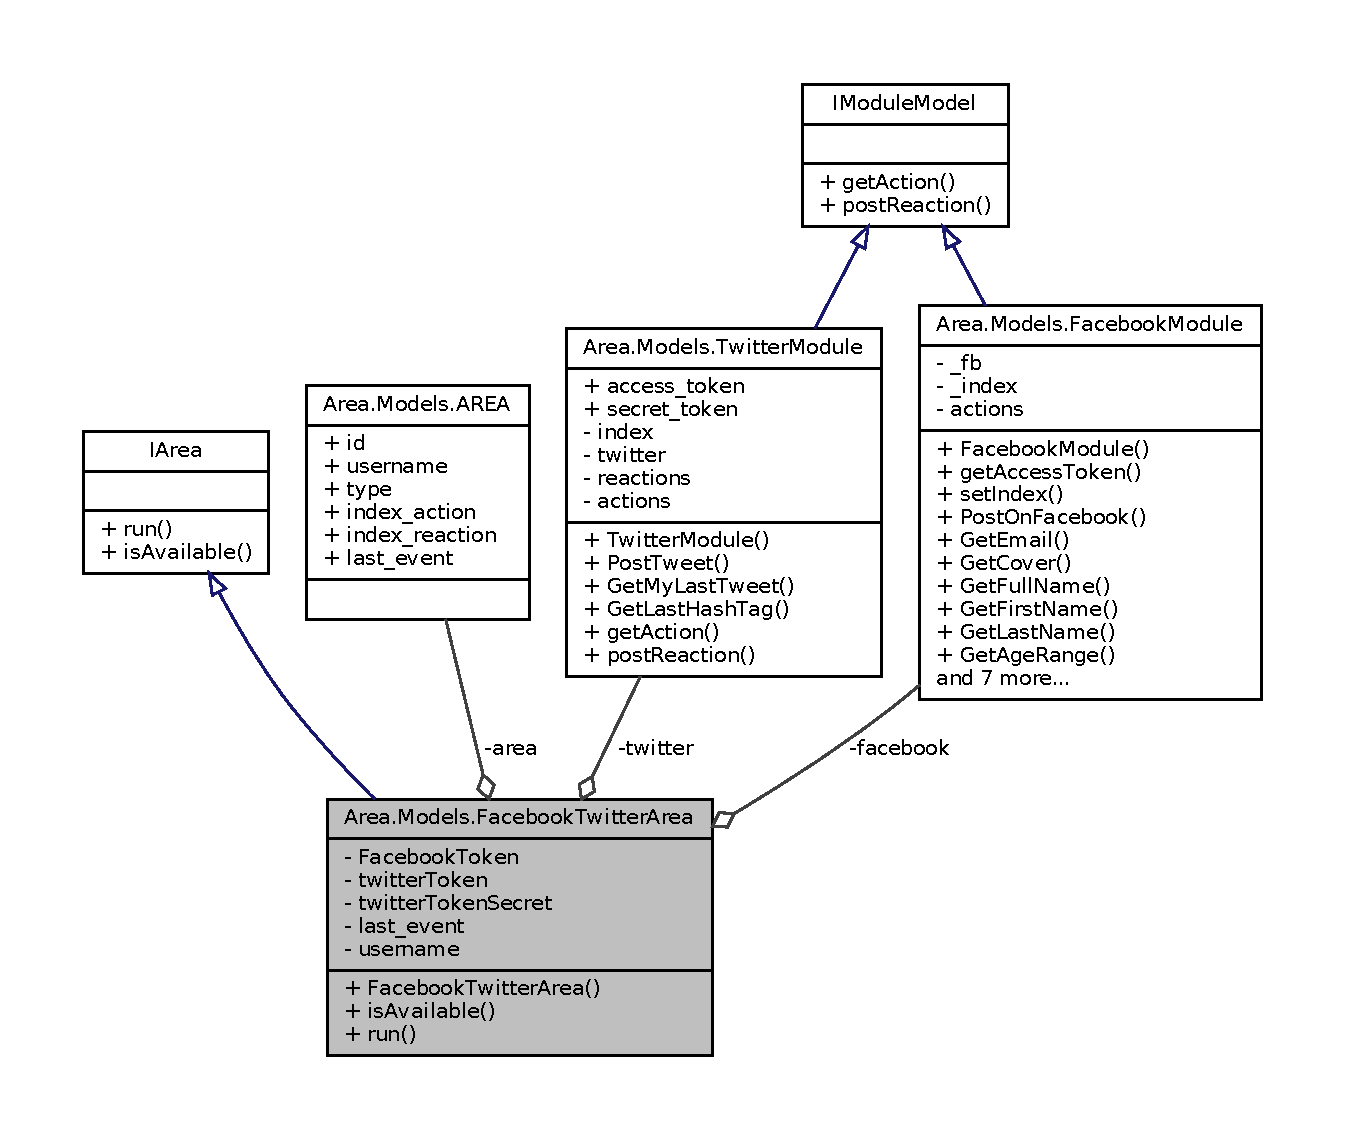
\includegraphics[width=350pt]{classArea_1_1Models_1_1FacebookTwitterArea__coll__graph}
\end{center}
\end{figure}
\subsection*{Public Member Functions}
\begin{DoxyCompactItemize}
\item 
\mbox{\hyperlink{classArea_1_1Models_1_1FacebookTwitterArea_a0dc27d5ece84c475eef593c6fa5bbf37}{Facebook\+Twitter\+Area}} (\mbox{\hyperlink{classArea_1_1Models_1_1AREA}{A\+R\+EA}} \mbox{\hyperlink{classArea_1_1Models_1_1FacebookTwitterArea_a6a3c4f7dbf8cf22fb47b567d0a0742bb}{area}}, \mbox{\hyperlink{classArea_1_1DAT_1_1AreaDbContext}{Area\+Db\+Context}} DB)
\item 
bool \mbox{\hyperlink{classArea_1_1Models_1_1FacebookTwitterArea_a654f1444c68fdbeb379c6df404b5b9f9}{is\+Available}} ()
\item 
void \mbox{\hyperlink{classArea_1_1Models_1_1FacebookTwitterArea_a6fd52c3124301206f73b8c9f025872d4}{run}} (\mbox{\hyperlink{classArea_1_1DAT_1_1AreaDbContext}{Area\+Db\+Context}} DB)
\end{DoxyCompactItemize}
\subsection*{Private Attributes}
\begin{DoxyCompactItemize}
\item 
\mbox{\hyperlink{classArea_1_1Models_1_1FacebookModule}{Facebook\+Module}} \mbox{\hyperlink{classArea_1_1Models_1_1FacebookTwitterArea_a7bfebac946d10f29dac8fc33449427af}{facebook}}
\item 
\mbox{\hyperlink{classArea_1_1Models_1_1TwitterModule}{Twitter\+Module}} \mbox{\hyperlink{classArea_1_1Models_1_1FacebookTwitterArea_acebc9b536cdd6cfa6cb99ea1a9f89b90}{twitter}}
\item 
string \mbox{\hyperlink{classArea_1_1Models_1_1FacebookTwitterArea_a701c427f5c067899221039ba7db5f5f6}{Facebook\+Token}} = \char`\"{}\char`\"{}
\item 
string \mbox{\hyperlink{classArea_1_1Models_1_1FacebookTwitterArea_ae05b7948cc24abc795d876b19f8aba89}{twitter\+Token}} = \char`\"{}\char`\"{}
\item 
string \mbox{\hyperlink{classArea_1_1Models_1_1FacebookTwitterArea_a79452d304aad4671b49c7d8045c75473}{twitter\+Token\+Secret}} = \char`\"{}\char`\"{}
\item 
string \mbox{\hyperlink{classArea_1_1Models_1_1FacebookTwitterArea_abf989aac27915851f2123dfa2fc39174}{last\+\_\+event}}
\item 
string \mbox{\hyperlink{classArea_1_1Models_1_1FacebookTwitterArea_ab361e159ba9a67bdd3f12fa0dac4b3a1}{username}}
\item 
\mbox{\hyperlink{classArea_1_1Models_1_1AREA}{A\+R\+EA}} \mbox{\hyperlink{classArea_1_1Models_1_1FacebookTwitterArea_a6a3c4f7dbf8cf22fb47b567d0a0742bb}{area}}
\end{DoxyCompactItemize}


\subsection{Constructor \& Destructor Documentation}
\mbox{\Hypertarget{classArea_1_1Models_1_1FacebookTwitterArea_a0dc27d5ece84c475eef593c6fa5bbf37}\label{classArea_1_1Models_1_1FacebookTwitterArea_a0dc27d5ece84c475eef593c6fa5bbf37}} 
\index{Area\+::\+Models\+::\+Facebook\+Twitter\+Area@{Area\+::\+Models\+::\+Facebook\+Twitter\+Area}!Facebook\+Twitter\+Area@{Facebook\+Twitter\+Area}}
\index{Facebook\+Twitter\+Area@{Facebook\+Twitter\+Area}!Area\+::\+Models\+::\+Facebook\+Twitter\+Area@{Area\+::\+Models\+::\+Facebook\+Twitter\+Area}}
\subsubsection{\texorpdfstring{Facebook\+Twitter\+Area()}{FacebookTwitterArea()}}
{\footnotesize\ttfamily Area.\+Models.\+Facebook\+Twitter\+Area.\+Facebook\+Twitter\+Area (\begin{DoxyParamCaption}\item[{\mbox{\hyperlink{classArea_1_1Models_1_1AREA}{A\+R\+EA}}}]{area,  }\item[{\mbox{\hyperlink{classArea_1_1DAT_1_1AreaDbContext}{Area\+Db\+Context}}}]{DB }\end{DoxyParamCaption})\hspace{0.3cm}{\ttfamily [inline]}}



\subsection{Member Function Documentation}
\mbox{\Hypertarget{classArea_1_1Models_1_1FacebookTwitterArea_a654f1444c68fdbeb379c6df404b5b9f9}\label{classArea_1_1Models_1_1FacebookTwitterArea_a654f1444c68fdbeb379c6df404b5b9f9}} 
\index{Area\+::\+Models\+::\+Facebook\+Twitter\+Area@{Area\+::\+Models\+::\+Facebook\+Twitter\+Area}!is\+Available@{is\+Available}}
\index{is\+Available@{is\+Available}!Area\+::\+Models\+::\+Facebook\+Twitter\+Area@{Area\+::\+Models\+::\+Facebook\+Twitter\+Area}}
\subsubsection{\texorpdfstring{is\+Available()}{isAvailable()}}
{\footnotesize\ttfamily bool Area.\+Models.\+Facebook\+Twitter\+Area.\+is\+Available (\begin{DoxyParamCaption}{ }\end{DoxyParamCaption})\hspace{0.3cm}{\ttfamily [inline]}}



Implements \mbox{\hyperlink{interfaceArea_1_1Models_1_1IArea_a742b324f0d7573f7f99f9e2adb5df94c}{Area.\+Models.\+I\+Area}}.

Here is the call graph for this function\+:
\nopagebreak
\begin{figure}[H]
\begin{center}
\leavevmode
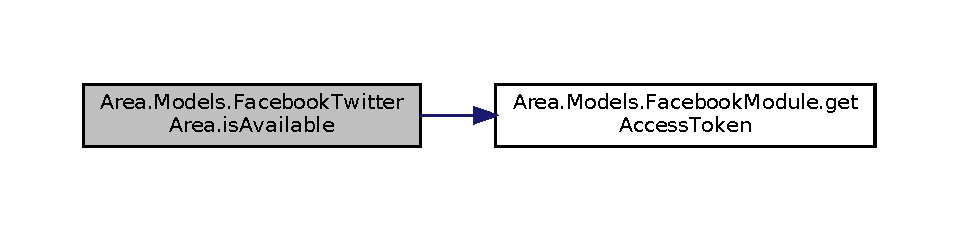
\includegraphics[width=350pt]{classArea_1_1Models_1_1FacebookTwitterArea_a654f1444c68fdbeb379c6df404b5b9f9_cgraph}
\end{center}
\end{figure}
\mbox{\Hypertarget{classArea_1_1Models_1_1FacebookTwitterArea_a6fd52c3124301206f73b8c9f025872d4}\label{classArea_1_1Models_1_1FacebookTwitterArea_a6fd52c3124301206f73b8c9f025872d4}} 
\index{Area\+::\+Models\+::\+Facebook\+Twitter\+Area@{Area\+::\+Models\+::\+Facebook\+Twitter\+Area}!run@{run}}
\index{run@{run}!Area\+::\+Models\+::\+Facebook\+Twitter\+Area@{Area\+::\+Models\+::\+Facebook\+Twitter\+Area}}
\subsubsection{\texorpdfstring{run()}{run()}}
{\footnotesize\ttfamily void Area.\+Models.\+Facebook\+Twitter\+Area.\+run (\begin{DoxyParamCaption}\item[{\mbox{\hyperlink{classArea_1_1DAT_1_1AreaDbContext}{Area\+Db\+Context}}}]{DB }\end{DoxyParamCaption})\hspace{0.3cm}{\ttfamily [inline]}}



Implements \mbox{\hyperlink{interfaceArea_1_1Models_1_1IArea_af153822d2715dad8eb1c250bcc4de567}{Area.\+Models.\+I\+Area}}.

Here is the call graph for this function\+:
\nopagebreak
\begin{figure}[H]
\begin{center}
\leavevmode
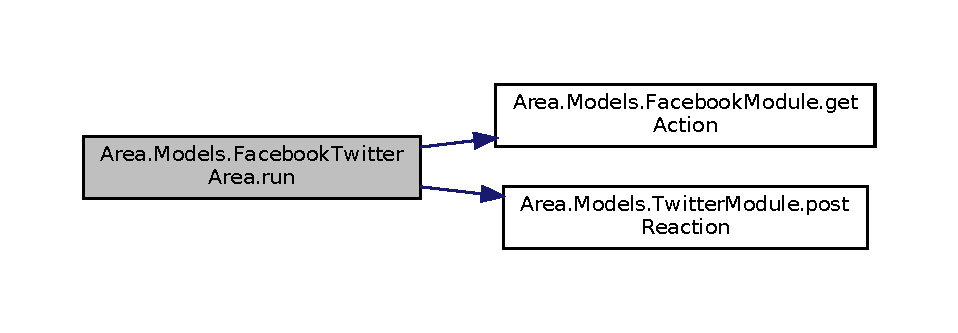
\includegraphics[width=350pt]{classArea_1_1Models_1_1FacebookTwitterArea_a6fd52c3124301206f73b8c9f025872d4_cgraph}
\end{center}
\end{figure}


\subsection{Member Data Documentation}
\mbox{\Hypertarget{classArea_1_1Models_1_1FacebookTwitterArea_a6a3c4f7dbf8cf22fb47b567d0a0742bb}\label{classArea_1_1Models_1_1FacebookTwitterArea_a6a3c4f7dbf8cf22fb47b567d0a0742bb}} 
\index{Area\+::\+Models\+::\+Facebook\+Twitter\+Area@{Area\+::\+Models\+::\+Facebook\+Twitter\+Area}!area@{area}}
\index{area@{area}!Area\+::\+Models\+::\+Facebook\+Twitter\+Area@{Area\+::\+Models\+::\+Facebook\+Twitter\+Area}}
\subsubsection{\texorpdfstring{area}{area}}
{\footnotesize\ttfamily \mbox{\hyperlink{classArea_1_1Models_1_1AREA}{A\+R\+EA}} Area.\+Models.\+Facebook\+Twitter\+Area.\+area\hspace{0.3cm}{\ttfamily [private]}}

\mbox{\Hypertarget{classArea_1_1Models_1_1FacebookTwitterArea_a7bfebac946d10f29dac8fc33449427af}\label{classArea_1_1Models_1_1FacebookTwitterArea_a7bfebac946d10f29dac8fc33449427af}} 
\index{Area\+::\+Models\+::\+Facebook\+Twitter\+Area@{Area\+::\+Models\+::\+Facebook\+Twitter\+Area}!facebook@{facebook}}
\index{facebook@{facebook}!Area\+::\+Models\+::\+Facebook\+Twitter\+Area@{Area\+::\+Models\+::\+Facebook\+Twitter\+Area}}
\subsubsection{\texorpdfstring{facebook}{facebook}}
{\footnotesize\ttfamily \mbox{\hyperlink{classArea_1_1Models_1_1FacebookModule}{Facebook\+Module}} Area.\+Models.\+Facebook\+Twitter\+Area.\+facebook\hspace{0.3cm}{\ttfamily [private]}}

\mbox{\Hypertarget{classArea_1_1Models_1_1FacebookTwitterArea_a701c427f5c067899221039ba7db5f5f6}\label{classArea_1_1Models_1_1FacebookTwitterArea_a701c427f5c067899221039ba7db5f5f6}} 
\index{Area\+::\+Models\+::\+Facebook\+Twitter\+Area@{Area\+::\+Models\+::\+Facebook\+Twitter\+Area}!Facebook\+Token@{Facebook\+Token}}
\index{Facebook\+Token@{Facebook\+Token}!Area\+::\+Models\+::\+Facebook\+Twitter\+Area@{Area\+::\+Models\+::\+Facebook\+Twitter\+Area}}
\subsubsection{\texorpdfstring{Facebook\+Token}{FacebookToken}}
{\footnotesize\ttfamily string Area.\+Models.\+Facebook\+Twitter\+Area.\+Facebook\+Token = \char`\"{}\char`\"{}\hspace{0.3cm}{\ttfamily [private]}}

\mbox{\Hypertarget{classArea_1_1Models_1_1FacebookTwitterArea_abf989aac27915851f2123dfa2fc39174}\label{classArea_1_1Models_1_1FacebookTwitterArea_abf989aac27915851f2123dfa2fc39174}} 
\index{Area\+::\+Models\+::\+Facebook\+Twitter\+Area@{Area\+::\+Models\+::\+Facebook\+Twitter\+Area}!last\+\_\+event@{last\+\_\+event}}
\index{last\+\_\+event@{last\+\_\+event}!Area\+::\+Models\+::\+Facebook\+Twitter\+Area@{Area\+::\+Models\+::\+Facebook\+Twitter\+Area}}
\subsubsection{\texorpdfstring{last\+\_\+event}{last\_event}}
{\footnotesize\ttfamily string Area.\+Models.\+Facebook\+Twitter\+Area.\+last\+\_\+event\hspace{0.3cm}{\ttfamily [private]}}

\mbox{\Hypertarget{classArea_1_1Models_1_1FacebookTwitterArea_acebc9b536cdd6cfa6cb99ea1a9f89b90}\label{classArea_1_1Models_1_1FacebookTwitterArea_acebc9b536cdd6cfa6cb99ea1a9f89b90}} 
\index{Area\+::\+Models\+::\+Facebook\+Twitter\+Area@{Area\+::\+Models\+::\+Facebook\+Twitter\+Area}!twitter@{twitter}}
\index{twitter@{twitter}!Area\+::\+Models\+::\+Facebook\+Twitter\+Area@{Area\+::\+Models\+::\+Facebook\+Twitter\+Area}}
\subsubsection{\texorpdfstring{twitter}{twitter}}
{\footnotesize\ttfamily \mbox{\hyperlink{classArea_1_1Models_1_1TwitterModule}{Twitter\+Module}} Area.\+Models.\+Facebook\+Twitter\+Area.\+twitter\hspace{0.3cm}{\ttfamily [private]}}

\mbox{\Hypertarget{classArea_1_1Models_1_1FacebookTwitterArea_ae05b7948cc24abc795d876b19f8aba89}\label{classArea_1_1Models_1_1FacebookTwitterArea_ae05b7948cc24abc795d876b19f8aba89}} 
\index{Area\+::\+Models\+::\+Facebook\+Twitter\+Area@{Area\+::\+Models\+::\+Facebook\+Twitter\+Area}!twitter\+Token@{twitter\+Token}}
\index{twitter\+Token@{twitter\+Token}!Area\+::\+Models\+::\+Facebook\+Twitter\+Area@{Area\+::\+Models\+::\+Facebook\+Twitter\+Area}}
\subsubsection{\texorpdfstring{twitter\+Token}{twitterToken}}
{\footnotesize\ttfamily string Area.\+Models.\+Facebook\+Twitter\+Area.\+twitter\+Token = \char`\"{}\char`\"{}\hspace{0.3cm}{\ttfamily [private]}}

\mbox{\Hypertarget{classArea_1_1Models_1_1FacebookTwitterArea_a79452d304aad4671b49c7d8045c75473}\label{classArea_1_1Models_1_1FacebookTwitterArea_a79452d304aad4671b49c7d8045c75473}} 
\index{Area\+::\+Models\+::\+Facebook\+Twitter\+Area@{Area\+::\+Models\+::\+Facebook\+Twitter\+Area}!twitter\+Token\+Secret@{twitter\+Token\+Secret}}
\index{twitter\+Token\+Secret@{twitter\+Token\+Secret}!Area\+::\+Models\+::\+Facebook\+Twitter\+Area@{Area\+::\+Models\+::\+Facebook\+Twitter\+Area}}
\subsubsection{\texorpdfstring{twitter\+Token\+Secret}{twitterTokenSecret}}
{\footnotesize\ttfamily string Area.\+Models.\+Facebook\+Twitter\+Area.\+twitter\+Token\+Secret = \char`\"{}\char`\"{}\hspace{0.3cm}{\ttfamily [private]}}

\mbox{\Hypertarget{classArea_1_1Models_1_1FacebookTwitterArea_ab361e159ba9a67bdd3f12fa0dac4b3a1}\label{classArea_1_1Models_1_1FacebookTwitterArea_ab361e159ba9a67bdd3f12fa0dac4b3a1}} 
\index{Area\+::\+Models\+::\+Facebook\+Twitter\+Area@{Area\+::\+Models\+::\+Facebook\+Twitter\+Area}!username@{username}}
\index{username@{username}!Area\+::\+Models\+::\+Facebook\+Twitter\+Area@{Area\+::\+Models\+::\+Facebook\+Twitter\+Area}}
\subsubsection{\texorpdfstring{username}{username}}
{\footnotesize\ttfamily string Area.\+Models.\+Facebook\+Twitter\+Area.\+username\hspace{0.3cm}{\ttfamily [private]}}



The documentation for this class was generated from the following file\+:\begin{DoxyCompactItemize}
\item 
Models/\+Areas/\mbox{\hyperlink{FacebookTwitterArea_8cs}{Facebook\+Twitter\+Area.\+cs}}\end{DoxyCompactItemize}

\hypertarget{classArea_1_1Controllers_1_1FacebookTwitterAreaController}{}\section{Area.\+Controllers.\+Facebook\+Twitter\+Area\+Controller Class Reference}
\label{classArea_1_1Controllers_1_1FacebookTwitterAreaController}\index{Area.\+Controllers.\+Facebook\+Twitter\+Area\+Controller@{Area.\+Controllers.\+Facebook\+Twitter\+Area\+Controller}}


Inheritance diagram for Area.\+Controllers.\+Facebook\+Twitter\+Area\+Controller\+:
\nopagebreak
\begin{figure}[H]
\begin{center}
\leavevmode
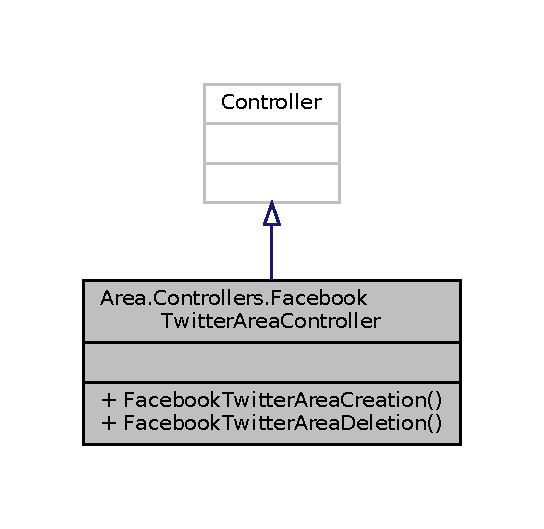
\includegraphics[width=261pt]{classArea_1_1Controllers_1_1FacebookTwitterAreaController__inherit__graph}
\end{center}
\end{figure}


Collaboration diagram for Area.\+Controllers.\+Facebook\+Twitter\+Area\+Controller\+:
\nopagebreak
\begin{figure}[H]
\begin{center}
\leavevmode
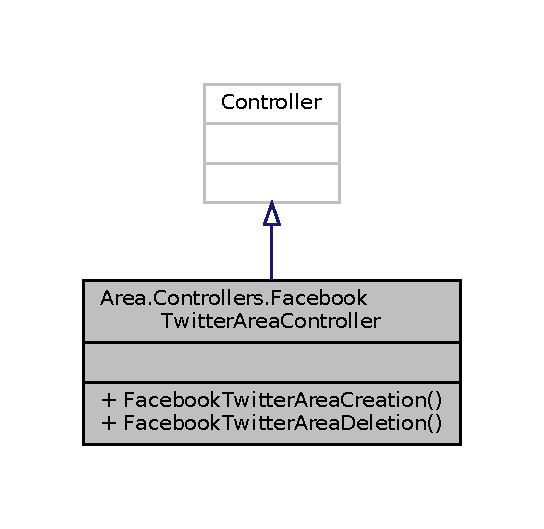
\includegraphics[width=261pt]{classArea_1_1Controllers_1_1FacebookTwitterAreaController__coll__graph}
\end{center}
\end{figure}
\subsection*{Public Member Functions}
\begin{DoxyCompactItemize}
\item 
Action\+Result \mbox{\hyperlink{classArea_1_1Controllers_1_1FacebookTwitterAreaController_a8b6d2384b234eaaae0ea4e8b2d87e8ed}{Facebook\+Twitter\+Area\+Creation}} (string action\+\_\+index, string reaction\+\_\+index, \mbox{[}From\+Services\mbox{]} \mbox{\hyperlink{classArea_1_1DAT_1_1AreaDbContext}{Area\+Db\+Context}} DB)
\item 
Action\+Result \mbox{\hyperlink{classArea_1_1Controllers_1_1FacebookTwitterAreaController_aaecd5ed1abd81974a4a00b6addec9a09}{Facebook\+Twitter\+Area\+Deletion}} (string action\+\_\+index, string reaction\+\_\+index, \mbox{[}From\+Services\mbox{]} \mbox{\hyperlink{classArea_1_1DAT_1_1AreaDbContext}{Area\+Db\+Context}} DB)
\end{DoxyCompactItemize}


\subsection{Member Function Documentation}
\mbox{\Hypertarget{classArea_1_1Controllers_1_1FacebookTwitterAreaController_a8b6d2384b234eaaae0ea4e8b2d87e8ed}\label{classArea_1_1Controllers_1_1FacebookTwitterAreaController_a8b6d2384b234eaaae0ea4e8b2d87e8ed}} 
\index{Area\+::\+Controllers\+::\+Facebook\+Twitter\+Area\+Controller@{Area\+::\+Controllers\+::\+Facebook\+Twitter\+Area\+Controller}!Facebook\+Twitter\+Area\+Creation@{Facebook\+Twitter\+Area\+Creation}}
\index{Facebook\+Twitter\+Area\+Creation@{Facebook\+Twitter\+Area\+Creation}!Area\+::\+Controllers\+::\+Facebook\+Twitter\+Area\+Controller@{Area\+::\+Controllers\+::\+Facebook\+Twitter\+Area\+Controller}}
\subsubsection{\texorpdfstring{Facebook\+Twitter\+Area\+Creation()}{FacebookTwitterAreaCreation()}}
{\footnotesize\ttfamily Action\+Result Area.\+Controllers.\+Facebook\+Twitter\+Area\+Controller.\+Facebook\+Twitter\+Area\+Creation (\begin{DoxyParamCaption}\item[{string}]{action\+\_\+index,  }\item[{string}]{reaction\+\_\+index,  }\item[{\mbox{[}\+From\+Services\mbox{]} \mbox{\hyperlink{classArea_1_1DAT_1_1AreaDbContext}{Area\+Db\+Context}}}]{DB }\end{DoxyParamCaption})\hspace{0.3cm}{\ttfamily [inline]}}

\mbox{\Hypertarget{classArea_1_1Controllers_1_1FacebookTwitterAreaController_aaecd5ed1abd81974a4a00b6addec9a09}\label{classArea_1_1Controllers_1_1FacebookTwitterAreaController_aaecd5ed1abd81974a4a00b6addec9a09}} 
\index{Area\+::\+Controllers\+::\+Facebook\+Twitter\+Area\+Controller@{Area\+::\+Controllers\+::\+Facebook\+Twitter\+Area\+Controller}!Facebook\+Twitter\+Area\+Deletion@{Facebook\+Twitter\+Area\+Deletion}}
\index{Facebook\+Twitter\+Area\+Deletion@{Facebook\+Twitter\+Area\+Deletion}!Area\+::\+Controllers\+::\+Facebook\+Twitter\+Area\+Controller@{Area\+::\+Controllers\+::\+Facebook\+Twitter\+Area\+Controller}}
\subsubsection{\texorpdfstring{Facebook\+Twitter\+Area\+Deletion()}{FacebookTwitterAreaDeletion()}}
{\footnotesize\ttfamily Action\+Result Area.\+Controllers.\+Facebook\+Twitter\+Area\+Controller.\+Facebook\+Twitter\+Area\+Deletion (\begin{DoxyParamCaption}\item[{string}]{action\+\_\+index,  }\item[{string}]{reaction\+\_\+index,  }\item[{\mbox{[}\+From\+Services\mbox{]} \mbox{\hyperlink{classArea_1_1DAT_1_1AreaDbContext}{Area\+Db\+Context}}}]{DB }\end{DoxyParamCaption})\hspace{0.3cm}{\ttfamily [inline]}}



The documentation for this class was generated from the following file\+:\begin{DoxyCompactItemize}
\item 
Controllers/\mbox{\hyperlink{FacebookTwitterAreaController_8cs}{Facebook\+Twitter\+Area\+Controller.\+cs}}\end{DoxyCompactItemize}

\hypertarget{classArea_1_1Models_1_1FormCode}{}\section{Area.\+Models.\+Form\+Code Class Reference}
\label{classArea_1_1Models_1_1FormCode}\index{Area.\+Models.\+Form\+Code@{Area.\+Models.\+Form\+Code}}


Collaboration diagram for Area.\+Models.\+Form\+Code\+:
\nopagebreak
\begin{figure}[H]
\begin{center}
\leavevmode
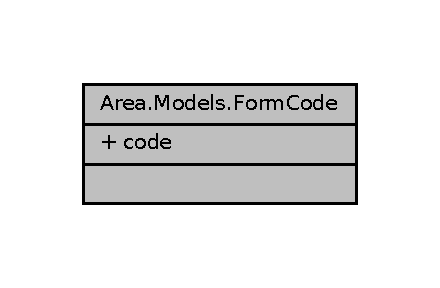
\includegraphics[width=211pt]{classArea_1_1Models_1_1FormCode__coll__graph}
\end{center}
\end{figure}
\subsection*{Properties}
\begin{DoxyCompactItemize}
\item 
string \mbox{\hyperlink{classArea_1_1Models_1_1FormCode_a44e5903ce56830e8acf23a558c27c4ef}{code}}\hspace{0.3cm}{\ttfamily  \mbox{[}get, set\mbox{]}}
\end{DoxyCompactItemize}


\subsection{Property Documentation}
\mbox{\Hypertarget{classArea_1_1Models_1_1FormCode_a44e5903ce56830e8acf23a558c27c4ef}\label{classArea_1_1Models_1_1FormCode_a44e5903ce56830e8acf23a558c27c4ef}} 
\index{Area\+::\+Models\+::\+Form\+Code@{Area\+::\+Models\+::\+Form\+Code}!code@{code}}
\index{code@{code}!Area\+::\+Models\+::\+Form\+Code@{Area\+::\+Models\+::\+Form\+Code}}
\subsubsection{\texorpdfstring{code}{code}}
{\footnotesize\ttfamily string Area.\+Models.\+Form\+Code.\+code\hspace{0.3cm}{\ttfamily [get]}, {\ttfamily [set]}}



The documentation for this class was generated from the following file\+:\begin{DoxyCompactItemize}
\item 
Models/\mbox{\hyperlink{FormModel_8cs}{Form\+Model.\+cs}}\end{DoxyCompactItemize}

\hypertarget{classArea_1_1Models_1_1FormLogin}{}\section{Area.\+Models.\+Form\+Login Class Reference}
\label{classArea_1_1Models_1_1FormLogin}\index{Area.\+Models.\+Form\+Login@{Area.\+Models.\+Form\+Login}}


Collaboration diagram for Area.\+Models.\+Form\+Login\+:
\nopagebreak
\begin{figure}[H]
\begin{center}
\leavevmode
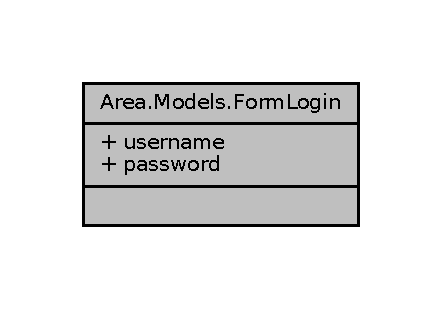
\includegraphics[width=212pt]{classArea_1_1Models_1_1FormLogin__coll__graph}
\end{center}
\end{figure}
\subsection*{Properties}
\begin{DoxyCompactItemize}
\item 
string \mbox{\hyperlink{classArea_1_1Models_1_1FormLogin_a4702f49df99650fe317cf8e02b721921}{username}}\hspace{0.3cm}{\ttfamily  \mbox{[}get, set\mbox{]}}
\item 
string \mbox{\hyperlink{classArea_1_1Models_1_1FormLogin_ab398fa2efd055aed5845781c47848821}{password}}\hspace{0.3cm}{\ttfamily  \mbox{[}get, set\mbox{]}}
\end{DoxyCompactItemize}


\subsection{Property Documentation}
\mbox{\Hypertarget{classArea_1_1Models_1_1FormLogin_ab398fa2efd055aed5845781c47848821}\label{classArea_1_1Models_1_1FormLogin_ab398fa2efd055aed5845781c47848821}} 
\index{Area\+::\+Models\+::\+Form\+Login@{Area\+::\+Models\+::\+Form\+Login}!password@{password}}
\index{password@{password}!Area\+::\+Models\+::\+Form\+Login@{Area\+::\+Models\+::\+Form\+Login}}
\subsubsection{\texorpdfstring{password}{password}}
{\footnotesize\ttfamily string Area.\+Models.\+Form\+Login.\+password\hspace{0.3cm}{\ttfamily [get]}, {\ttfamily [set]}}

\mbox{\Hypertarget{classArea_1_1Models_1_1FormLogin_a4702f49df99650fe317cf8e02b721921}\label{classArea_1_1Models_1_1FormLogin_a4702f49df99650fe317cf8e02b721921}} 
\index{Area\+::\+Models\+::\+Form\+Login@{Area\+::\+Models\+::\+Form\+Login}!username@{username}}
\index{username@{username}!Area\+::\+Models\+::\+Form\+Login@{Area\+::\+Models\+::\+Form\+Login}}
\subsubsection{\texorpdfstring{username}{username}}
{\footnotesize\ttfamily string Area.\+Models.\+Form\+Login.\+username\hspace{0.3cm}{\ttfamily [get]}, {\ttfamily [set]}}



The documentation for this class was generated from the following file\+:\begin{DoxyCompactItemize}
\item 
Models/\mbox{\hyperlink{FormModel_8cs}{Form\+Model.\+cs}}\end{DoxyCompactItemize}

\hypertarget{classArea_1_1Models_1_1FormRegister}{}\section{Area.\+Models.\+Form\+Register Class Reference}
\label{classArea_1_1Models_1_1FormRegister}\index{Area.\+Models.\+Form\+Register@{Area.\+Models.\+Form\+Register}}


Collaboration diagram for Area.\+Models.\+Form\+Register\+:
\nopagebreak
\begin{figure}[H]
\begin{center}
\leavevmode
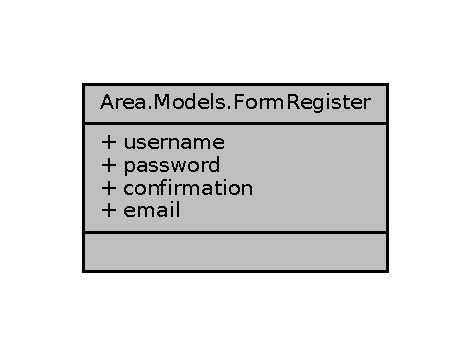
\includegraphics[width=226pt]{classArea_1_1Models_1_1FormRegister__coll__graph}
\end{center}
\end{figure}
\subsection*{Properties}
\begin{DoxyCompactItemize}
\item 
string \mbox{\hyperlink{classArea_1_1Models_1_1FormRegister_a065f953c377405bee288651cf6cec86c}{username}}\hspace{0.3cm}{\ttfamily  \mbox{[}get, set\mbox{]}}
\item 
string \mbox{\hyperlink{classArea_1_1Models_1_1FormRegister_a329d7035be225b4713412da0a4f0cbe1}{password}}\hspace{0.3cm}{\ttfamily  \mbox{[}get, set\mbox{]}}
\item 
string \mbox{\hyperlink{classArea_1_1Models_1_1FormRegister_a2bb8a77816c4952485a8821dc17fc5af}{confirmation}}\hspace{0.3cm}{\ttfamily  \mbox{[}get, set\mbox{]}}
\item 
string \mbox{\hyperlink{classArea_1_1Models_1_1FormRegister_a57e3da2ac200f01b6cb4a1ac90cedd1b}{email}}\hspace{0.3cm}{\ttfamily  \mbox{[}get, set\mbox{]}}
\end{DoxyCompactItemize}


\subsection{Property Documentation}
\mbox{\Hypertarget{classArea_1_1Models_1_1FormRegister_a2bb8a77816c4952485a8821dc17fc5af}\label{classArea_1_1Models_1_1FormRegister_a2bb8a77816c4952485a8821dc17fc5af}} 
\index{Area\+::\+Models\+::\+Form\+Register@{Area\+::\+Models\+::\+Form\+Register}!confirmation@{confirmation}}
\index{confirmation@{confirmation}!Area\+::\+Models\+::\+Form\+Register@{Area\+::\+Models\+::\+Form\+Register}}
\subsubsection{\texorpdfstring{confirmation}{confirmation}}
{\footnotesize\ttfamily string Area.\+Models.\+Form\+Register.\+confirmation\hspace{0.3cm}{\ttfamily [get]}, {\ttfamily [set]}}

\mbox{\Hypertarget{classArea_1_1Models_1_1FormRegister_a57e3da2ac200f01b6cb4a1ac90cedd1b}\label{classArea_1_1Models_1_1FormRegister_a57e3da2ac200f01b6cb4a1ac90cedd1b}} 
\index{Area\+::\+Models\+::\+Form\+Register@{Area\+::\+Models\+::\+Form\+Register}!email@{email}}
\index{email@{email}!Area\+::\+Models\+::\+Form\+Register@{Area\+::\+Models\+::\+Form\+Register}}
\subsubsection{\texorpdfstring{email}{email}}
{\footnotesize\ttfamily string Area.\+Models.\+Form\+Register.\+email\hspace{0.3cm}{\ttfamily [get]}, {\ttfamily [set]}}

\mbox{\Hypertarget{classArea_1_1Models_1_1FormRegister_a329d7035be225b4713412da0a4f0cbe1}\label{classArea_1_1Models_1_1FormRegister_a329d7035be225b4713412da0a4f0cbe1}} 
\index{Area\+::\+Models\+::\+Form\+Register@{Area\+::\+Models\+::\+Form\+Register}!password@{password}}
\index{password@{password}!Area\+::\+Models\+::\+Form\+Register@{Area\+::\+Models\+::\+Form\+Register}}
\subsubsection{\texorpdfstring{password}{password}}
{\footnotesize\ttfamily string Area.\+Models.\+Form\+Register.\+password\hspace{0.3cm}{\ttfamily [get]}, {\ttfamily [set]}}

\mbox{\Hypertarget{classArea_1_1Models_1_1FormRegister_a065f953c377405bee288651cf6cec86c}\label{classArea_1_1Models_1_1FormRegister_a065f953c377405bee288651cf6cec86c}} 
\index{Area\+::\+Models\+::\+Form\+Register@{Area\+::\+Models\+::\+Form\+Register}!username@{username}}
\index{username@{username}!Area\+::\+Models\+::\+Form\+Register@{Area\+::\+Models\+::\+Form\+Register}}
\subsubsection{\texorpdfstring{username}{username}}
{\footnotesize\ttfamily string Area.\+Models.\+Form\+Register.\+username\hspace{0.3cm}{\ttfamily [get]}, {\ttfamily [set]}}



The documentation for this class was generated from the following file\+:\begin{DoxyCompactItemize}
\item 
Models/\mbox{\hyperlink{FormModel_8cs}{Form\+Model.\+cs}}\end{DoxyCompactItemize}

\hypertarget{classArea_1_1Controllers_1_1GithubController}{}\section{Area.\+Controllers.\+Github\+Controller Class Reference}
\label{classArea_1_1Controllers_1_1GithubController}\index{Area.\+Controllers.\+Github\+Controller@{Area.\+Controllers.\+Github\+Controller}}


Inheritance diagram for Area.\+Controllers.\+Github\+Controller\+:
\nopagebreak
\begin{figure}[H]
\begin{center}
\leavevmode
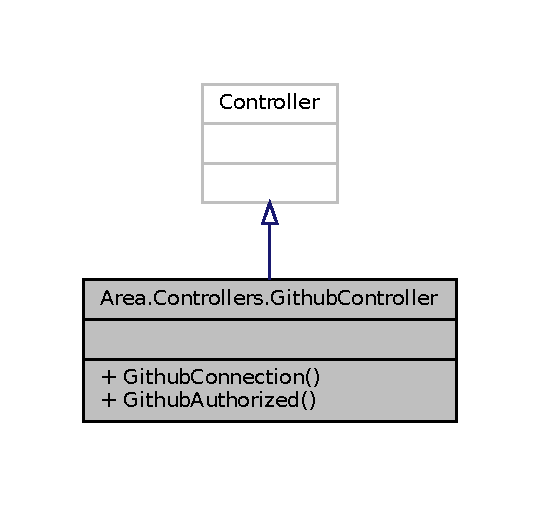
\includegraphics[width=259pt]{classArea_1_1Controllers_1_1GithubController__inherit__graph}
\end{center}
\end{figure}


Collaboration diagram for Area.\+Controllers.\+Github\+Controller\+:
\nopagebreak
\begin{figure}[H]
\begin{center}
\leavevmode
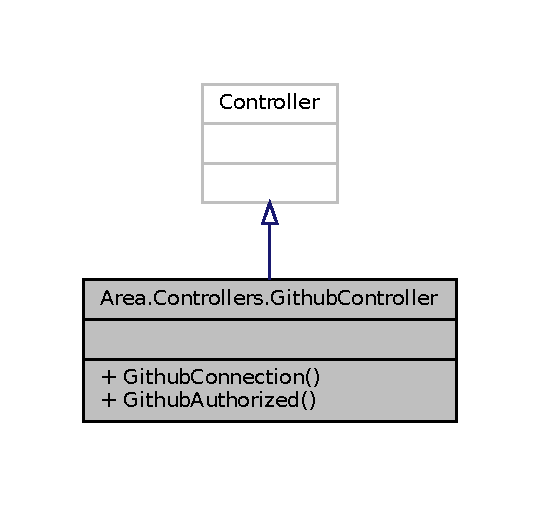
\includegraphics[width=259pt]{classArea_1_1Controllers_1_1GithubController__coll__graph}
\end{center}
\end{figure}
\subsection*{Public Member Functions}
\begin{DoxyCompactItemize}
\item 
Action\+Result \mbox{\hyperlink{classArea_1_1Controllers_1_1GithubController_ae09ff800b4a3caa6450c7004197c5a90}{Github\+Connection}} ()
\item 
async Task$<$ Action\+Result $>$ \mbox{\hyperlink{classArea_1_1Controllers_1_1GithubController_a785ec72735634312f473455a0858e91b}{Github\+Authorized}} (string code, string state, \mbox{[}From\+Services\mbox{]} \mbox{\hyperlink{classArea_1_1DAT_1_1AreaDbContext}{Area\+Db\+Context}} DB)
\end{DoxyCompactItemize}


\subsection{Member Function Documentation}
\mbox{\Hypertarget{classArea_1_1Controllers_1_1GithubController_a785ec72735634312f473455a0858e91b}\label{classArea_1_1Controllers_1_1GithubController_a785ec72735634312f473455a0858e91b}} 
\index{Area\+::\+Controllers\+::\+Github\+Controller@{Area\+::\+Controllers\+::\+Github\+Controller}!Github\+Authorized@{Github\+Authorized}}
\index{Github\+Authorized@{Github\+Authorized}!Area\+::\+Controllers\+::\+Github\+Controller@{Area\+::\+Controllers\+::\+Github\+Controller}}
\subsubsection{\texorpdfstring{Github\+Authorized()}{GithubAuthorized()}}
{\footnotesize\ttfamily async Task$<$Action\+Result$>$ Area.\+Controllers.\+Github\+Controller.\+Github\+Authorized (\begin{DoxyParamCaption}\item[{string}]{code,  }\item[{string}]{state,  }\item[{\mbox{[}\+From\+Services\mbox{]} \mbox{\hyperlink{classArea_1_1DAT_1_1AreaDbContext}{Area\+Db\+Context}}}]{DB }\end{DoxyParamCaption})\hspace{0.3cm}{\ttfamily [inline]}}

\mbox{\Hypertarget{classArea_1_1Controllers_1_1GithubController_ae09ff800b4a3caa6450c7004197c5a90}\label{classArea_1_1Controllers_1_1GithubController_ae09ff800b4a3caa6450c7004197c5a90}} 
\index{Area\+::\+Controllers\+::\+Github\+Controller@{Area\+::\+Controllers\+::\+Github\+Controller}!Github\+Connection@{Github\+Connection}}
\index{Github\+Connection@{Github\+Connection}!Area\+::\+Controllers\+::\+Github\+Controller@{Area\+::\+Controllers\+::\+Github\+Controller}}
\subsubsection{\texorpdfstring{Github\+Connection()}{GithubConnection()}}
{\footnotesize\ttfamily Action\+Result Area.\+Controllers.\+Github\+Controller.\+Github\+Connection (\begin{DoxyParamCaption}{ }\end{DoxyParamCaption})\hspace{0.3cm}{\ttfamily [inline]}}



The documentation for this class was generated from the following file\+:\begin{DoxyCompactItemize}
\item 
Controllers/\mbox{\hyperlink{GithubController_8cs}{Github\+Controller.\+cs}}\end{DoxyCompactItemize}

\hypertarget{classArea_1_1Models_1_1GithubFacebookArea}{}\section{Area.\+Models.\+Github\+Facebook\+Area Class Reference}
\label{classArea_1_1Models_1_1GithubFacebookArea}\index{Area.\+Models.\+Github\+Facebook\+Area@{Area.\+Models.\+Github\+Facebook\+Area}}


Inheritance diagram for Area.\+Models.\+Github\+Facebook\+Area\+:
\nopagebreak
\begin{figure}[H]
\begin{center}
\leavevmode
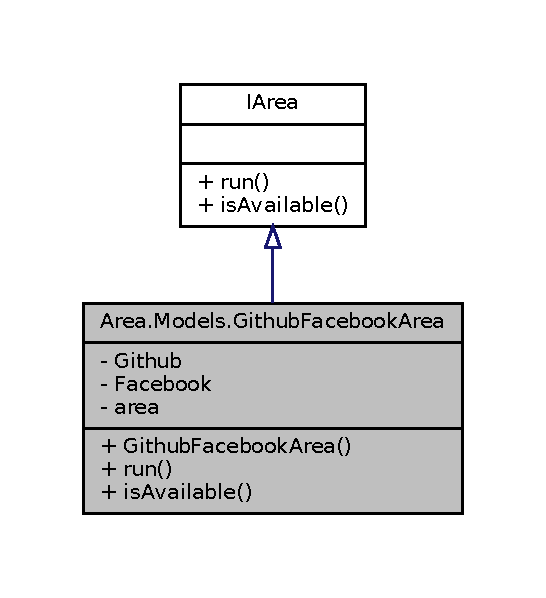
\includegraphics[width=262pt]{classArea_1_1Models_1_1GithubFacebookArea__inherit__graph}
\end{center}
\end{figure}


Collaboration diagram for Area.\+Models.\+Github\+Facebook\+Area\+:
\nopagebreak
\begin{figure}[H]
\begin{center}
\leavevmode
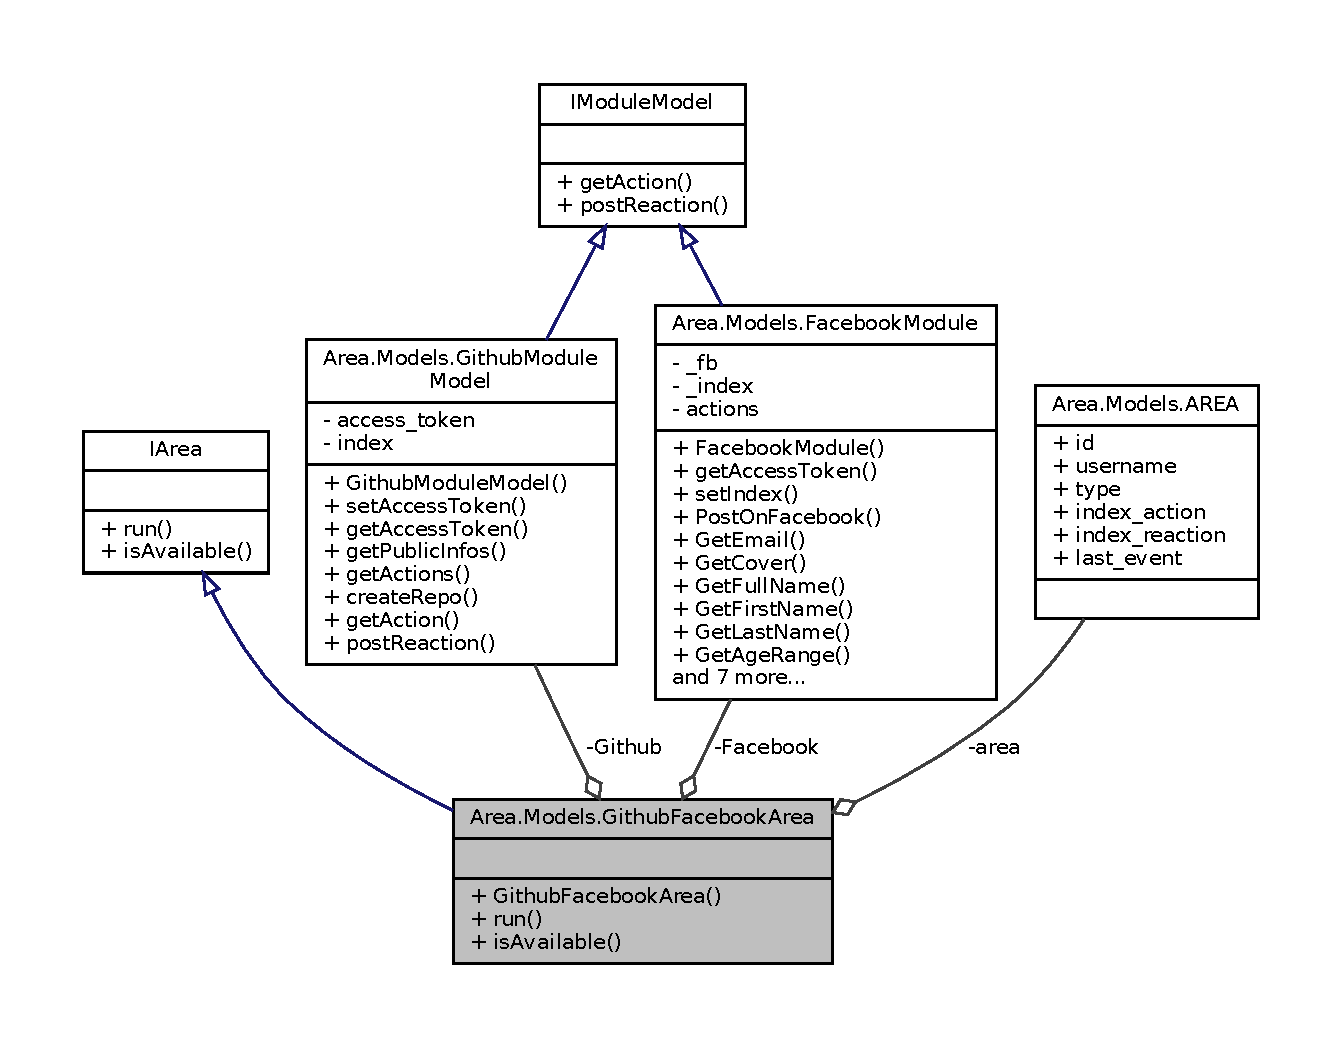
\includegraphics[width=350pt]{classArea_1_1Models_1_1GithubFacebookArea__coll__graph}
\end{center}
\end{figure}
\subsection*{Public Member Functions}
\begin{DoxyCompactItemize}
\item 
\mbox{\hyperlink{classArea_1_1Models_1_1GithubFacebookArea_a233779b2e51c30dbbfc24051c8bad602}{Github\+Facebook\+Area}} (\mbox{\hyperlink{classArea_1_1Models_1_1AREA}{A\+R\+EA}} \mbox{\hyperlink{classArea_1_1Models_1_1GithubFacebookArea_a4ab3d7c1e18136e3d9b22b640cb3e052}{area}}, \mbox{\hyperlink{classArea_1_1DAT_1_1AreaDbContext}{Area\+Db\+Context}} DB)
\item 
void \mbox{\hyperlink{classArea_1_1Models_1_1GithubFacebookArea_a984d46335dd21d81088312ebe413a0fc}{run}} (\mbox{\hyperlink{classArea_1_1DAT_1_1AreaDbContext}{Area\+Db\+Context}} DB)
\item 
bool \mbox{\hyperlink{classArea_1_1Models_1_1GithubFacebookArea_ab1f22cb94018e33fa92221c812da1020}{is\+Available}} ()
\end{DoxyCompactItemize}
\subsection*{Private Attributes}
\begin{DoxyCompactItemize}
\item 
\mbox{\hyperlink{classArea_1_1Models_1_1GithubModuleModel}{Github\+Module\+Model}} \mbox{\hyperlink{classArea_1_1Models_1_1GithubFacebookArea_a5ff7826b5d7f7578cabc0b0e0ab79646}{Github}}
\item 
\mbox{\hyperlink{classArea_1_1Models_1_1FacebookModule}{Facebook\+Module}} \mbox{\hyperlink{classArea_1_1Models_1_1GithubFacebookArea_af5f388eaff8394ef70a57a38f3e1e065}{Facebook}}
\item 
\mbox{\hyperlink{classArea_1_1Models_1_1AREA}{A\+R\+EA}} \mbox{\hyperlink{classArea_1_1Models_1_1GithubFacebookArea_a4ab3d7c1e18136e3d9b22b640cb3e052}{area}}
\end{DoxyCompactItemize}


\subsection{Constructor \& Destructor Documentation}
\mbox{\Hypertarget{classArea_1_1Models_1_1GithubFacebookArea_a233779b2e51c30dbbfc24051c8bad602}\label{classArea_1_1Models_1_1GithubFacebookArea_a233779b2e51c30dbbfc24051c8bad602}} 
\index{Area\+::\+Models\+::\+Github\+Facebook\+Area@{Area\+::\+Models\+::\+Github\+Facebook\+Area}!Github\+Facebook\+Area@{Github\+Facebook\+Area}}
\index{Github\+Facebook\+Area@{Github\+Facebook\+Area}!Area\+::\+Models\+::\+Github\+Facebook\+Area@{Area\+::\+Models\+::\+Github\+Facebook\+Area}}
\subsubsection{\texorpdfstring{Github\+Facebook\+Area()}{GithubFacebookArea()}}
{\footnotesize\ttfamily Area.\+Models.\+Github\+Facebook\+Area.\+Github\+Facebook\+Area (\begin{DoxyParamCaption}\item[{\mbox{\hyperlink{classArea_1_1Models_1_1AREA}{A\+R\+EA}}}]{area,  }\item[{\mbox{\hyperlink{classArea_1_1DAT_1_1AreaDbContext}{Area\+Db\+Context}}}]{DB }\end{DoxyParamCaption})\hspace{0.3cm}{\ttfamily [inline]}}



\subsection{Member Function Documentation}
\mbox{\Hypertarget{classArea_1_1Models_1_1GithubFacebookArea_ab1f22cb94018e33fa92221c812da1020}\label{classArea_1_1Models_1_1GithubFacebookArea_ab1f22cb94018e33fa92221c812da1020}} 
\index{Area\+::\+Models\+::\+Github\+Facebook\+Area@{Area\+::\+Models\+::\+Github\+Facebook\+Area}!is\+Available@{is\+Available}}
\index{is\+Available@{is\+Available}!Area\+::\+Models\+::\+Github\+Facebook\+Area@{Area\+::\+Models\+::\+Github\+Facebook\+Area}}
\subsubsection{\texorpdfstring{is\+Available()}{isAvailable()}}
{\footnotesize\ttfamily bool Area.\+Models.\+Github\+Facebook\+Area.\+is\+Available (\begin{DoxyParamCaption}{ }\end{DoxyParamCaption})\hspace{0.3cm}{\ttfamily [inline]}}



Implements \mbox{\hyperlink{interfaceArea_1_1Models_1_1IArea_a742b324f0d7573f7f99f9e2adb5df94c}{Area.\+Models.\+I\+Area}}.

Here is the call graph for this function\+:
\nopagebreak
\begin{figure}[H]
\begin{center}
\leavevmode
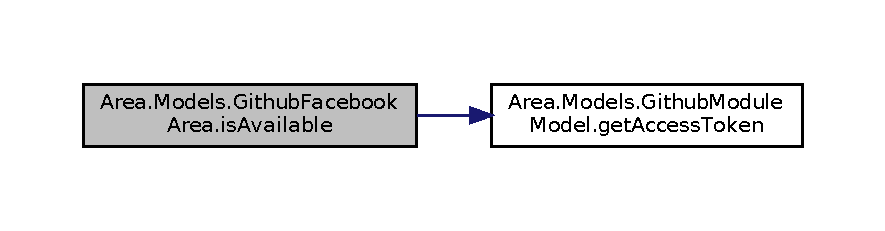
\includegraphics[width=350pt]{classArea_1_1Models_1_1GithubFacebookArea_ab1f22cb94018e33fa92221c812da1020_cgraph}
\end{center}
\end{figure}
\mbox{\Hypertarget{classArea_1_1Models_1_1GithubFacebookArea_a984d46335dd21d81088312ebe413a0fc}\label{classArea_1_1Models_1_1GithubFacebookArea_a984d46335dd21d81088312ebe413a0fc}} 
\index{Area\+::\+Models\+::\+Github\+Facebook\+Area@{Area\+::\+Models\+::\+Github\+Facebook\+Area}!run@{run}}
\index{run@{run}!Area\+::\+Models\+::\+Github\+Facebook\+Area@{Area\+::\+Models\+::\+Github\+Facebook\+Area}}
\subsubsection{\texorpdfstring{run()}{run()}}
{\footnotesize\ttfamily void Area.\+Models.\+Github\+Facebook\+Area.\+run (\begin{DoxyParamCaption}\item[{\mbox{\hyperlink{classArea_1_1DAT_1_1AreaDbContext}{Area\+Db\+Context}}}]{DB }\end{DoxyParamCaption})\hspace{0.3cm}{\ttfamily [inline]}}



Implements \mbox{\hyperlink{interfaceArea_1_1Models_1_1IArea_af153822d2715dad8eb1c250bcc4de567}{Area.\+Models.\+I\+Area}}.

Here is the call graph for this function\+:
\nopagebreak
\begin{figure}[H]
\begin{center}
\leavevmode
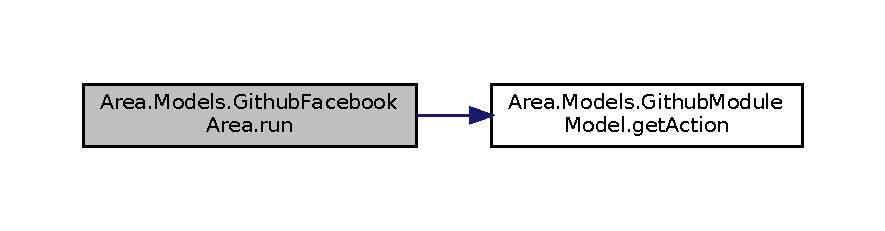
\includegraphics[width=350pt]{classArea_1_1Models_1_1GithubFacebookArea_a984d46335dd21d81088312ebe413a0fc_cgraph}
\end{center}
\end{figure}


\subsection{Member Data Documentation}
\mbox{\Hypertarget{classArea_1_1Models_1_1GithubFacebookArea_a4ab3d7c1e18136e3d9b22b640cb3e052}\label{classArea_1_1Models_1_1GithubFacebookArea_a4ab3d7c1e18136e3d9b22b640cb3e052}} 
\index{Area\+::\+Models\+::\+Github\+Facebook\+Area@{Area\+::\+Models\+::\+Github\+Facebook\+Area}!area@{area}}
\index{area@{area}!Area\+::\+Models\+::\+Github\+Facebook\+Area@{Area\+::\+Models\+::\+Github\+Facebook\+Area}}
\subsubsection{\texorpdfstring{area}{area}}
{\footnotesize\ttfamily \mbox{\hyperlink{classArea_1_1Models_1_1AREA}{A\+R\+EA}} Area.\+Models.\+Github\+Facebook\+Area.\+area\hspace{0.3cm}{\ttfamily [private]}}

\mbox{\Hypertarget{classArea_1_1Models_1_1GithubFacebookArea_af5f388eaff8394ef70a57a38f3e1e065}\label{classArea_1_1Models_1_1GithubFacebookArea_af5f388eaff8394ef70a57a38f3e1e065}} 
\index{Area\+::\+Models\+::\+Github\+Facebook\+Area@{Area\+::\+Models\+::\+Github\+Facebook\+Area}!Facebook@{Facebook}}
\index{Facebook@{Facebook}!Area\+::\+Models\+::\+Github\+Facebook\+Area@{Area\+::\+Models\+::\+Github\+Facebook\+Area}}
\subsubsection{\texorpdfstring{Facebook}{Facebook}}
{\footnotesize\ttfamily \mbox{\hyperlink{classArea_1_1Models_1_1FacebookModule}{Facebook\+Module}} Area.\+Models.\+Github\+Facebook\+Area.\+Facebook\hspace{0.3cm}{\ttfamily [private]}}

\mbox{\Hypertarget{classArea_1_1Models_1_1GithubFacebookArea_a5ff7826b5d7f7578cabc0b0e0ab79646}\label{classArea_1_1Models_1_1GithubFacebookArea_a5ff7826b5d7f7578cabc0b0e0ab79646}} 
\index{Area\+::\+Models\+::\+Github\+Facebook\+Area@{Area\+::\+Models\+::\+Github\+Facebook\+Area}!Github@{Github}}
\index{Github@{Github}!Area\+::\+Models\+::\+Github\+Facebook\+Area@{Area\+::\+Models\+::\+Github\+Facebook\+Area}}
\subsubsection{\texorpdfstring{Github}{Github}}
{\footnotesize\ttfamily \mbox{\hyperlink{classArea_1_1Models_1_1GithubModuleModel}{Github\+Module\+Model}} Area.\+Models.\+Github\+Facebook\+Area.\+Github\hspace{0.3cm}{\ttfamily [private]}}



The documentation for this class was generated from the following file\+:\begin{DoxyCompactItemize}
\item 
Models/\+Areas/\mbox{\hyperlink{GithubFacebookArea_8cs}{Github\+Facebook\+Area.\+cs}}\end{DoxyCompactItemize}

\hypertarget{classArea_1_1Controllers_1_1GithubFacebookAreaController}{}\section{Area.\+Controllers.\+Github\+Facebook\+Area\+Controller Class Reference}
\label{classArea_1_1Controllers_1_1GithubFacebookAreaController}\index{Area.\+Controllers.\+Github\+Facebook\+Area\+Controller@{Area.\+Controllers.\+Github\+Facebook\+Area\+Controller}}


Inheritance diagram for Area.\+Controllers.\+Github\+Facebook\+Area\+Controller\+:
\nopagebreak
\begin{figure}[H]
\begin{center}
\leavevmode
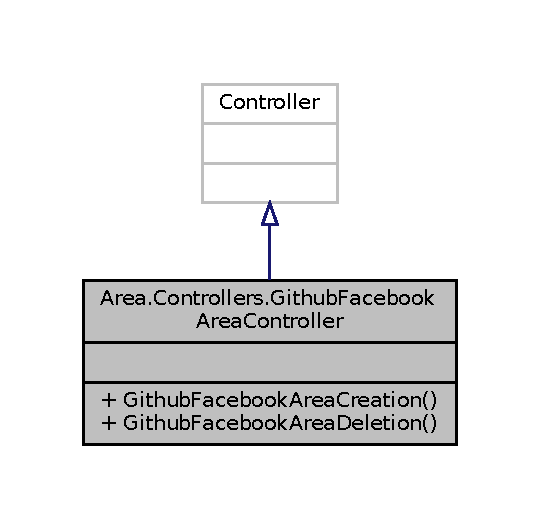
\includegraphics[width=259pt]{classArea_1_1Controllers_1_1GithubFacebookAreaController__inherit__graph}
\end{center}
\end{figure}


Collaboration diagram for Area.\+Controllers.\+Github\+Facebook\+Area\+Controller\+:
\nopagebreak
\begin{figure}[H]
\begin{center}
\leavevmode
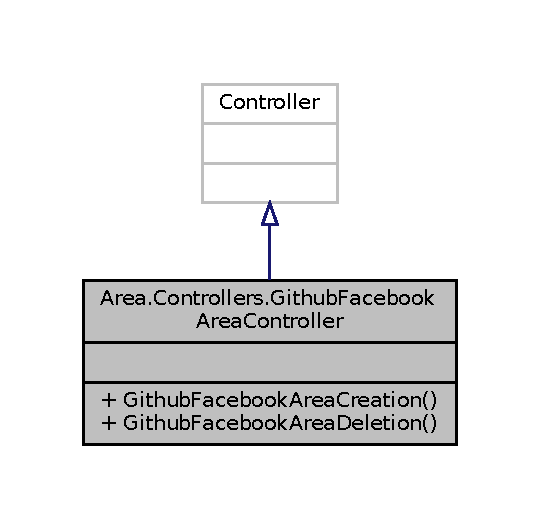
\includegraphics[width=259pt]{classArea_1_1Controllers_1_1GithubFacebookAreaController__coll__graph}
\end{center}
\end{figure}
\subsection*{Public Member Functions}
\begin{DoxyCompactItemize}
\item 
Action\+Result \mbox{\hyperlink{classArea_1_1Controllers_1_1GithubFacebookAreaController_a77c51d433cb771e27be9db12ab7dc16f}{Github\+Facebook\+Area\+Creation}} (string action\+\_\+index, string reaction\+\_\+index, \mbox{[}From\+Services\mbox{]} \mbox{\hyperlink{classArea_1_1DAT_1_1AreaDbContext}{Area\+Db\+Context}} DB)
\item 
Action\+Result \mbox{\hyperlink{classArea_1_1Controllers_1_1GithubFacebookAreaController_a8611f6f02f968f08b14a1888a84900b7}{Github\+Facebook\+Area\+Deletion}} (string action\+\_\+index, string reaction\+\_\+index, \mbox{[}From\+Services\mbox{]} \mbox{\hyperlink{classArea_1_1DAT_1_1AreaDbContext}{Area\+Db\+Context}} DB)
\end{DoxyCompactItemize}


\subsection{Member Function Documentation}
\mbox{\Hypertarget{classArea_1_1Controllers_1_1GithubFacebookAreaController_a77c51d433cb771e27be9db12ab7dc16f}\label{classArea_1_1Controllers_1_1GithubFacebookAreaController_a77c51d433cb771e27be9db12ab7dc16f}} 
\index{Area\+::\+Controllers\+::\+Github\+Facebook\+Area\+Controller@{Area\+::\+Controllers\+::\+Github\+Facebook\+Area\+Controller}!Github\+Facebook\+Area\+Creation@{Github\+Facebook\+Area\+Creation}}
\index{Github\+Facebook\+Area\+Creation@{Github\+Facebook\+Area\+Creation}!Area\+::\+Controllers\+::\+Github\+Facebook\+Area\+Controller@{Area\+::\+Controllers\+::\+Github\+Facebook\+Area\+Controller}}
\subsubsection{\texorpdfstring{Github\+Facebook\+Area\+Creation()}{GithubFacebookAreaCreation()}}
{\footnotesize\ttfamily Action\+Result Area.\+Controllers.\+Github\+Facebook\+Area\+Controller.\+Github\+Facebook\+Area\+Creation (\begin{DoxyParamCaption}\item[{string}]{action\+\_\+index,  }\item[{string}]{reaction\+\_\+index,  }\item[{\mbox{[}\+From\+Services\mbox{]} \mbox{\hyperlink{classArea_1_1DAT_1_1AreaDbContext}{Area\+Db\+Context}}}]{DB }\end{DoxyParamCaption})\hspace{0.3cm}{\ttfamily [inline]}}

\mbox{\Hypertarget{classArea_1_1Controllers_1_1GithubFacebookAreaController_a8611f6f02f968f08b14a1888a84900b7}\label{classArea_1_1Controllers_1_1GithubFacebookAreaController_a8611f6f02f968f08b14a1888a84900b7}} 
\index{Area\+::\+Controllers\+::\+Github\+Facebook\+Area\+Controller@{Area\+::\+Controllers\+::\+Github\+Facebook\+Area\+Controller}!Github\+Facebook\+Area\+Deletion@{Github\+Facebook\+Area\+Deletion}}
\index{Github\+Facebook\+Area\+Deletion@{Github\+Facebook\+Area\+Deletion}!Area\+::\+Controllers\+::\+Github\+Facebook\+Area\+Controller@{Area\+::\+Controllers\+::\+Github\+Facebook\+Area\+Controller}}
\subsubsection{\texorpdfstring{Github\+Facebook\+Area\+Deletion()}{GithubFacebookAreaDeletion()}}
{\footnotesize\ttfamily Action\+Result Area.\+Controllers.\+Github\+Facebook\+Area\+Controller.\+Github\+Facebook\+Area\+Deletion (\begin{DoxyParamCaption}\item[{string}]{action\+\_\+index,  }\item[{string}]{reaction\+\_\+index,  }\item[{\mbox{[}\+From\+Services\mbox{]} \mbox{\hyperlink{classArea_1_1DAT_1_1AreaDbContext}{Area\+Db\+Context}}}]{DB }\end{DoxyParamCaption})\hspace{0.3cm}{\ttfamily [inline]}}



The documentation for this class was generated from the following file\+:\begin{DoxyCompactItemize}
\item 
Controllers/\mbox{\hyperlink{GithubFacebookAreaController_8cs}{Github\+Facebook\+Area\+Controller.\+cs}}\end{DoxyCompactItemize}

\hypertarget{classArea_1_1Models_1_1GithubModuleModel}{}\section{Area.\+Models.\+Github\+Module\+Model Class Reference}
\label{classArea_1_1Models_1_1GithubModuleModel}\index{Area.\+Models.\+Github\+Module\+Model@{Area.\+Models.\+Github\+Module\+Model}}


Inheritance diagram for Area.\+Models.\+Github\+Module\+Model\+:
\nopagebreak
\begin{figure}[H]
\begin{center}
\leavevmode
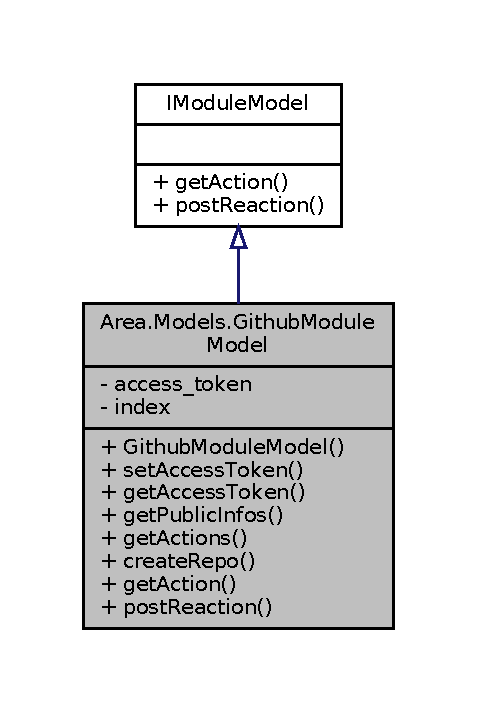
\includegraphics[width=229pt]{classArea_1_1Models_1_1GithubModuleModel__inherit__graph}
\end{center}
\end{figure}


Collaboration diagram for Area.\+Models.\+Github\+Module\+Model\+:
\nopagebreak
\begin{figure}[H]
\begin{center}
\leavevmode
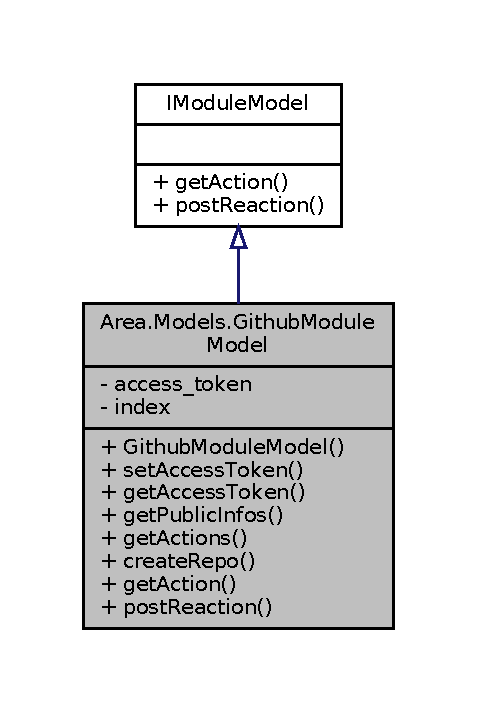
\includegraphics[width=229pt]{classArea_1_1Models_1_1GithubModuleModel__coll__graph}
\end{center}
\end{figure}
\subsection*{Public Member Functions}
\begin{DoxyCompactItemize}
\item 
\mbox{\hyperlink{classArea_1_1Models_1_1GithubModuleModel_a33a887e8a0eef8e83cf284f573376e0c}{Github\+Module\+Model}} (string token, int \mbox{\hyperlink{classArea_1_1Models_1_1GithubModuleModel_a6264559445da398186a78c81b0ad0a06}{index}})
\item 
void \mbox{\hyperlink{classArea_1_1Models_1_1GithubModuleModel_a71c393a20452dff06a57b49b97a50e0d}{set\+Access\+Token}} (string token)
\item 
string \mbox{\hyperlink{classArea_1_1Models_1_1GithubModuleModel_ac7ee8eda979a73d787ca6418320822be}{get\+Access\+Token}} ()
\item 
async Task$<$ Dictionary$<$ string, string $>$ $>$ \mbox{\hyperlink{classArea_1_1Models_1_1GithubModuleModel_a39fa05affc8836f1f10d7b95a0c0669a}{get\+Public\+Infos}} ()
\item 
async Task$<$ Dictionary$<$ int, string $>$ $>$ \mbox{\hyperlink{classArea_1_1Models_1_1GithubModuleModel_af3b210b6f977264dfdf3dfb1bf56cb1a}{get\+Actions}} ()
\item 
async void \mbox{\hyperlink{classArea_1_1Models_1_1GithubModuleModel_a1c4790c05ecfacd3d4979d4817b201d8}{create\+Repo}} (string name)
\item 
string \mbox{\hyperlink{classArea_1_1Models_1_1GithubModuleModel_aebec4ccbd02441daa062ce936a9f4e3d}{get\+Action}} ()
\item 
void \mbox{\hyperlink{classArea_1_1Models_1_1GithubModuleModel_aeeda0ad6ec3b9ddaa5a38e9b8a2ef020}{post\+Reaction}} (string reaction)
\end{DoxyCompactItemize}
\subsection*{Private Attributes}
\begin{DoxyCompactItemize}
\item 
string \mbox{\hyperlink{classArea_1_1Models_1_1GithubModuleModel_aae14b69d8630f1c9dfbf04ee3763e31b}{access\+\_\+token}}
\item 
int \mbox{\hyperlink{classArea_1_1Models_1_1GithubModuleModel_a6264559445da398186a78c81b0ad0a06}{index}}
\end{DoxyCompactItemize}


\subsection{Constructor \& Destructor Documentation}
\mbox{\Hypertarget{classArea_1_1Models_1_1GithubModuleModel_a33a887e8a0eef8e83cf284f573376e0c}\label{classArea_1_1Models_1_1GithubModuleModel_a33a887e8a0eef8e83cf284f573376e0c}} 
\index{Area\+::\+Models\+::\+Github\+Module\+Model@{Area\+::\+Models\+::\+Github\+Module\+Model}!Github\+Module\+Model@{Github\+Module\+Model}}
\index{Github\+Module\+Model@{Github\+Module\+Model}!Area\+::\+Models\+::\+Github\+Module\+Model@{Area\+::\+Models\+::\+Github\+Module\+Model}}
\subsubsection{\texorpdfstring{Github\+Module\+Model()}{GithubModuleModel()}}
{\footnotesize\ttfamily Area.\+Models.\+Github\+Module\+Model.\+Github\+Module\+Model (\begin{DoxyParamCaption}\item[{string}]{token,  }\item[{int}]{index }\end{DoxyParamCaption})\hspace{0.3cm}{\ttfamily [inline]}}



\subsection{Member Function Documentation}
\mbox{\Hypertarget{classArea_1_1Models_1_1GithubModuleModel_a1c4790c05ecfacd3d4979d4817b201d8}\label{classArea_1_1Models_1_1GithubModuleModel_a1c4790c05ecfacd3d4979d4817b201d8}} 
\index{Area\+::\+Models\+::\+Github\+Module\+Model@{Area\+::\+Models\+::\+Github\+Module\+Model}!create\+Repo@{create\+Repo}}
\index{create\+Repo@{create\+Repo}!Area\+::\+Models\+::\+Github\+Module\+Model@{Area\+::\+Models\+::\+Github\+Module\+Model}}
\subsubsection{\texorpdfstring{create\+Repo()}{createRepo()}}
{\footnotesize\ttfamily async void Area.\+Models.\+Github\+Module\+Model.\+create\+Repo (\begin{DoxyParamCaption}\item[{string}]{name }\end{DoxyParamCaption})\hspace{0.3cm}{\ttfamily [inline]}}

\mbox{\Hypertarget{classArea_1_1Models_1_1GithubModuleModel_ac7ee8eda979a73d787ca6418320822be}\label{classArea_1_1Models_1_1GithubModuleModel_ac7ee8eda979a73d787ca6418320822be}} 
\index{Area\+::\+Models\+::\+Github\+Module\+Model@{Area\+::\+Models\+::\+Github\+Module\+Model}!get\+Access\+Token@{get\+Access\+Token}}
\index{get\+Access\+Token@{get\+Access\+Token}!Area\+::\+Models\+::\+Github\+Module\+Model@{Area\+::\+Models\+::\+Github\+Module\+Model}}
\subsubsection{\texorpdfstring{get\+Access\+Token()}{getAccessToken()}}
{\footnotesize\ttfamily string Area.\+Models.\+Github\+Module\+Model.\+get\+Access\+Token (\begin{DoxyParamCaption}{ }\end{DoxyParamCaption})\hspace{0.3cm}{\ttfamily [inline]}}

\mbox{\Hypertarget{classArea_1_1Models_1_1GithubModuleModel_aebec4ccbd02441daa062ce936a9f4e3d}\label{classArea_1_1Models_1_1GithubModuleModel_aebec4ccbd02441daa062ce936a9f4e3d}} 
\index{Area\+::\+Models\+::\+Github\+Module\+Model@{Area\+::\+Models\+::\+Github\+Module\+Model}!get\+Action@{get\+Action}}
\index{get\+Action@{get\+Action}!Area\+::\+Models\+::\+Github\+Module\+Model@{Area\+::\+Models\+::\+Github\+Module\+Model}}
\subsubsection{\texorpdfstring{get\+Action()}{getAction()}}
{\footnotesize\ttfamily string Area.\+Models.\+Github\+Module\+Model.\+get\+Action (\begin{DoxyParamCaption}{ }\end{DoxyParamCaption})\hspace{0.3cm}{\ttfamily [inline]}}



Implements \mbox{\hyperlink{interfaceArea_1_1Models_1_1IModuleModel_a050d892fae9f85c6b607a7c0e30502e9}{Area.\+Models.\+I\+Module\+Model}}.

\mbox{\Hypertarget{classArea_1_1Models_1_1GithubModuleModel_af3b210b6f977264dfdf3dfb1bf56cb1a}\label{classArea_1_1Models_1_1GithubModuleModel_af3b210b6f977264dfdf3dfb1bf56cb1a}} 
\index{Area\+::\+Models\+::\+Github\+Module\+Model@{Area\+::\+Models\+::\+Github\+Module\+Model}!get\+Actions@{get\+Actions}}
\index{get\+Actions@{get\+Actions}!Area\+::\+Models\+::\+Github\+Module\+Model@{Area\+::\+Models\+::\+Github\+Module\+Model}}
\subsubsection{\texorpdfstring{get\+Actions()}{getActions()}}
{\footnotesize\ttfamily async Task$<$Dictionary$<$int, string$>$ $>$ Area.\+Models.\+Github\+Module\+Model.\+get\+Actions (\begin{DoxyParamCaption}{ }\end{DoxyParamCaption})\hspace{0.3cm}{\ttfamily [inline]}}

\mbox{\Hypertarget{classArea_1_1Models_1_1GithubModuleModel_a39fa05affc8836f1f10d7b95a0c0669a}\label{classArea_1_1Models_1_1GithubModuleModel_a39fa05affc8836f1f10d7b95a0c0669a}} 
\index{Area\+::\+Models\+::\+Github\+Module\+Model@{Area\+::\+Models\+::\+Github\+Module\+Model}!get\+Public\+Infos@{get\+Public\+Infos}}
\index{get\+Public\+Infos@{get\+Public\+Infos}!Area\+::\+Models\+::\+Github\+Module\+Model@{Area\+::\+Models\+::\+Github\+Module\+Model}}
\subsubsection{\texorpdfstring{get\+Public\+Infos()}{getPublicInfos()}}
{\footnotesize\ttfamily async Task$<$Dictionary$<$string, string$>$ $>$ Area.\+Models.\+Github\+Module\+Model.\+get\+Public\+Infos (\begin{DoxyParamCaption}{ }\end{DoxyParamCaption})\hspace{0.3cm}{\ttfamily [inline]}}

\mbox{\Hypertarget{classArea_1_1Models_1_1GithubModuleModel_aeeda0ad6ec3b9ddaa5a38e9b8a2ef020}\label{classArea_1_1Models_1_1GithubModuleModel_aeeda0ad6ec3b9ddaa5a38e9b8a2ef020}} 
\index{Area\+::\+Models\+::\+Github\+Module\+Model@{Area\+::\+Models\+::\+Github\+Module\+Model}!post\+Reaction@{post\+Reaction}}
\index{post\+Reaction@{post\+Reaction}!Area\+::\+Models\+::\+Github\+Module\+Model@{Area\+::\+Models\+::\+Github\+Module\+Model}}
\subsubsection{\texorpdfstring{post\+Reaction()}{postReaction()}}
{\footnotesize\ttfamily void Area.\+Models.\+Github\+Module\+Model.\+post\+Reaction (\begin{DoxyParamCaption}\item[{string}]{reaction }\end{DoxyParamCaption})\hspace{0.3cm}{\ttfamily [inline]}}



Implements \mbox{\hyperlink{interfaceArea_1_1Models_1_1IModuleModel_af2c1a82bd894255ab2099440f4f3d6f7}{Area.\+Models.\+I\+Module\+Model}}.

\mbox{\Hypertarget{classArea_1_1Models_1_1GithubModuleModel_a71c393a20452dff06a57b49b97a50e0d}\label{classArea_1_1Models_1_1GithubModuleModel_a71c393a20452dff06a57b49b97a50e0d}} 
\index{Area\+::\+Models\+::\+Github\+Module\+Model@{Area\+::\+Models\+::\+Github\+Module\+Model}!set\+Access\+Token@{set\+Access\+Token}}
\index{set\+Access\+Token@{set\+Access\+Token}!Area\+::\+Models\+::\+Github\+Module\+Model@{Area\+::\+Models\+::\+Github\+Module\+Model}}
\subsubsection{\texorpdfstring{set\+Access\+Token()}{setAccessToken()}}
{\footnotesize\ttfamily void Area.\+Models.\+Github\+Module\+Model.\+set\+Access\+Token (\begin{DoxyParamCaption}\item[{string}]{token }\end{DoxyParamCaption})\hspace{0.3cm}{\ttfamily [inline]}}



\subsection{Member Data Documentation}
\mbox{\Hypertarget{classArea_1_1Models_1_1GithubModuleModel_aae14b69d8630f1c9dfbf04ee3763e31b}\label{classArea_1_1Models_1_1GithubModuleModel_aae14b69d8630f1c9dfbf04ee3763e31b}} 
\index{Area\+::\+Models\+::\+Github\+Module\+Model@{Area\+::\+Models\+::\+Github\+Module\+Model}!access\+\_\+token@{access\+\_\+token}}
\index{access\+\_\+token@{access\+\_\+token}!Area\+::\+Models\+::\+Github\+Module\+Model@{Area\+::\+Models\+::\+Github\+Module\+Model}}
\subsubsection{\texorpdfstring{access\+\_\+token}{access\_token}}
{\footnotesize\ttfamily string Area.\+Models.\+Github\+Module\+Model.\+access\+\_\+token\hspace{0.3cm}{\ttfamily [private]}}

\mbox{\Hypertarget{classArea_1_1Models_1_1GithubModuleModel_a6264559445da398186a78c81b0ad0a06}\label{classArea_1_1Models_1_1GithubModuleModel_a6264559445da398186a78c81b0ad0a06}} 
\index{Area\+::\+Models\+::\+Github\+Module\+Model@{Area\+::\+Models\+::\+Github\+Module\+Model}!index@{index}}
\index{index@{index}!Area\+::\+Models\+::\+Github\+Module\+Model@{Area\+::\+Models\+::\+Github\+Module\+Model}}
\subsubsection{\texorpdfstring{index}{index}}
{\footnotesize\ttfamily int Area.\+Models.\+Github\+Module\+Model.\+index\hspace{0.3cm}{\ttfamily [private]}}



The documentation for this class was generated from the following file\+:\begin{DoxyCompactItemize}
\item 
Models/\+Modules/\mbox{\hyperlink{GithubModuleModel_8cs}{Github\+Module\+Model.\+cs}}\end{DoxyCompactItemize}

\hypertarget{classArea_1_1Controllers_1_1HomeController}{}\section{Area.\+Controllers.\+Home\+Controller Class Reference}
\label{classArea_1_1Controllers_1_1HomeController}\index{Area.\+Controllers.\+Home\+Controller@{Area.\+Controllers.\+Home\+Controller}}


Inheritance diagram for Area.\+Controllers.\+Home\+Controller\+:
\nopagebreak
\begin{figure}[H]
\begin{center}
\leavevmode
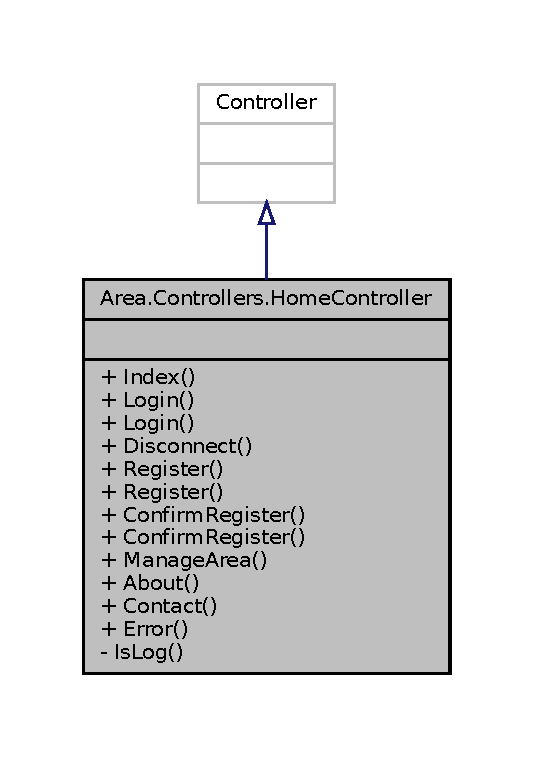
\includegraphics[width=256pt]{classArea_1_1Controllers_1_1HomeController__inherit__graph}
\end{center}
\end{figure}


Collaboration diagram for Area.\+Controllers.\+Home\+Controller\+:
\nopagebreak
\begin{figure}[H]
\begin{center}
\leavevmode
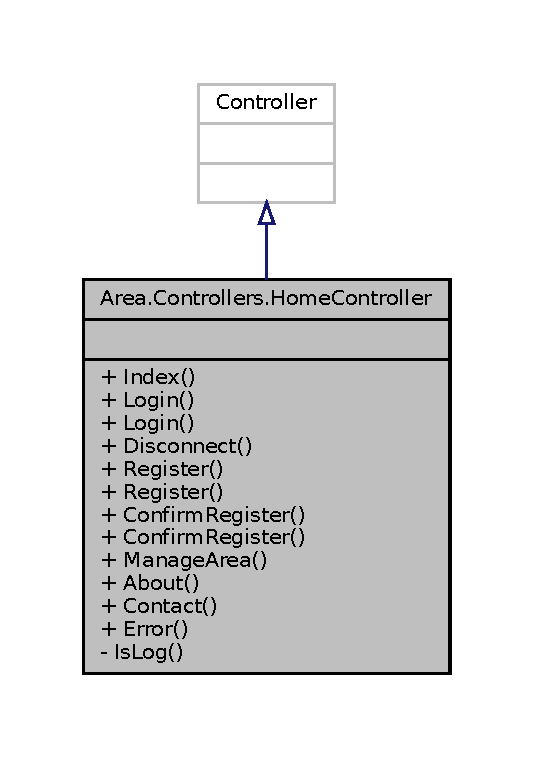
\includegraphics[width=256pt]{classArea_1_1Controllers_1_1HomeController__coll__graph}
\end{center}
\end{figure}
\subsection*{Public Member Functions}
\begin{DoxyCompactItemize}
\item 
I\+Action\+Result \mbox{\hyperlink{classArea_1_1Controllers_1_1HomeController_a81852c6564831c3ba0cf7eddfc354997}{Index}} (\mbox{[}From\+Services\mbox{]} \mbox{\hyperlink{classArea_1_1DAT_1_1AreaDbContext}{Area\+Db\+Context}} DB)
\item 
I\+Action\+Result \mbox{\hyperlink{classArea_1_1Controllers_1_1HomeController_a5e4cf8ba8004592c197e31621233ff79}{Login}} (\mbox{[}From\+Services\mbox{]} \mbox{\hyperlink{classArea_1_1DAT_1_1AreaDbContext}{Area\+Db\+Context}} DB)
\item 
I\+Action\+Result \mbox{\hyperlink{classArea_1_1Controllers_1_1HomeController_a998f5002ebee5cf5ae63d206b816cd8c}{Login}} (\mbox{[}From\+Services\mbox{]} \mbox{\hyperlink{classArea_1_1DAT_1_1AreaDbContext}{Area\+Db\+Context}} DB, \mbox{\hyperlink{classArea_1_1Models_1_1FormLogin}{Form\+Login}} model)
\item 
I\+Action\+Result \mbox{\hyperlink{classArea_1_1Controllers_1_1HomeController_a99eb071c86613ccfe8003b803bceaafe}{Disconnect}} (\mbox{[}From\+Services\mbox{]} \mbox{\hyperlink{classArea_1_1DAT_1_1AreaDbContext}{Area\+Db\+Context}} db\+Context)
\item 
I\+Action\+Result \mbox{\hyperlink{classArea_1_1Controllers_1_1HomeController_a3ed060342c26dee6645dfc7bc0204f09}{Register}} (\mbox{[}From\+Services\mbox{]} \mbox{\hyperlink{classArea_1_1DAT_1_1AreaDbContext}{Area\+Db\+Context}} DB)
\item 
I\+Action\+Result \mbox{\hyperlink{classArea_1_1Controllers_1_1HomeController_a3062b0baba8394d263dca4bb3a19427a}{Register}} (\mbox{[}From\+Services\mbox{]} \mbox{\hyperlink{classArea_1_1DAT_1_1AreaDbContext}{Area\+Db\+Context}} DB, \mbox{\hyperlink{classArea_1_1Models_1_1FormRegister}{Form\+Register}} model)
\item 
I\+Action\+Result \mbox{\hyperlink{classArea_1_1Controllers_1_1HomeController_a510df0d8145d5ffcf8e89369b86e478c}{Confirm\+Register}} (\mbox{[}From\+Services\mbox{]} \mbox{\hyperlink{classArea_1_1DAT_1_1AreaDbContext}{Area\+Db\+Context}} DB)
\item 
I\+Action\+Result \mbox{\hyperlink{classArea_1_1Controllers_1_1HomeController_a5e8c1711863dc28e3ec574f69aab79c5}{Confirm\+Register}} (\mbox{[}From\+Services\mbox{]} \mbox{\hyperlink{classArea_1_1DAT_1_1AreaDbContext}{Area\+Db\+Context}} DB, \mbox{\hyperlink{classArea_1_1Models_1_1FormCode}{Form\+Code}} model)
\item 
I\+Action\+Result \mbox{\hyperlink{classArea_1_1Controllers_1_1HomeController_a31ceb7fc34f6e2dec98d5b4e5989d3c7}{Manage\+Area}} (\mbox{[}From\+Services\mbox{]} \mbox{\hyperlink{classArea_1_1DAT_1_1AreaDbContext}{Area\+Db\+Context}} DB)
\item 
I\+Action\+Result \mbox{\hyperlink{classArea_1_1Controllers_1_1HomeController_a03e00eab1b1bef6f33369d61e8b9eacd}{About}} (\mbox{[}From\+Services\mbox{]} \mbox{\hyperlink{classArea_1_1DAT_1_1AreaDbContext}{Area\+Db\+Context}} DB)
\item 
I\+Action\+Result \mbox{\hyperlink{classArea_1_1Controllers_1_1HomeController_a029ed46ea5f2e8c9481d9c20f38b7875}{Contact}} (\mbox{[}From\+Services\mbox{]} \mbox{\hyperlink{classArea_1_1DAT_1_1AreaDbContext}{Area\+Db\+Context}} DB)
\item 
I\+Action\+Result \mbox{\hyperlink{classArea_1_1Controllers_1_1HomeController_a5770addb80c3fbaf23c159086b4c13d4}{Error}} ()
\end{DoxyCompactItemize}
\subsection*{Private Member Functions}
\begin{DoxyCompactItemize}
\item 
bool \mbox{\hyperlink{classArea_1_1Controllers_1_1HomeController_a41a57542642ed1c4b052975954a0794b}{Is\+Log}} (\mbox{[}From\+Services\mbox{]} \mbox{\hyperlink{classArea_1_1DAT_1_1AreaDbContext}{Area\+Db\+Context}} DB)
\end{DoxyCompactItemize}


\subsection{Member Function Documentation}
\mbox{\Hypertarget{classArea_1_1Controllers_1_1HomeController_a03e00eab1b1bef6f33369d61e8b9eacd}\label{classArea_1_1Controllers_1_1HomeController_a03e00eab1b1bef6f33369d61e8b9eacd}} 
\index{Area\+::\+Controllers\+::\+Home\+Controller@{Area\+::\+Controllers\+::\+Home\+Controller}!About@{About}}
\index{About@{About}!Area\+::\+Controllers\+::\+Home\+Controller@{Area\+::\+Controllers\+::\+Home\+Controller}}
\subsubsection{\texorpdfstring{About()}{About()}}
{\footnotesize\ttfamily I\+Action\+Result Area.\+Controllers.\+Home\+Controller.\+About (\begin{DoxyParamCaption}\item[{\mbox{[}\+From\+Services\mbox{]} \mbox{\hyperlink{classArea_1_1DAT_1_1AreaDbContext}{Area\+Db\+Context}}}]{DB }\end{DoxyParamCaption})\hspace{0.3cm}{\ttfamily [inline]}}

\mbox{\Hypertarget{classArea_1_1Controllers_1_1HomeController_a510df0d8145d5ffcf8e89369b86e478c}\label{classArea_1_1Controllers_1_1HomeController_a510df0d8145d5ffcf8e89369b86e478c}} 
\index{Area\+::\+Controllers\+::\+Home\+Controller@{Area\+::\+Controllers\+::\+Home\+Controller}!Confirm\+Register@{Confirm\+Register}}
\index{Confirm\+Register@{Confirm\+Register}!Area\+::\+Controllers\+::\+Home\+Controller@{Area\+::\+Controllers\+::\+Home\+Controller}}
\subsubsection{\texorpdfstring{Confirm\+Register()}{ConfirmRegister()}\hspace{0.1cm}{\footnotesize\ttfamily [1/2]}}
{\footnotesize\ttfamily I\+Action\+Result Area.\+Controllers.\+Home\+Controller.\+Confirm\+Register (\begin{DoxyParamCaption}\item[{\mbox{[}\+From\+Services\mbox{]} \mbox{\hyperlink{classArea_1_1DAT_1_1AreaDbContext}{Area\+Db\+Context}}}]{DB }\end{DoxyParamCaption})\hspace{0.3cm}{\ttfamily [inline]}}

Here is the call graph for this function\+:
\nopagebreak
\begin{figure}[H]
\begin{center}
\leavevmode
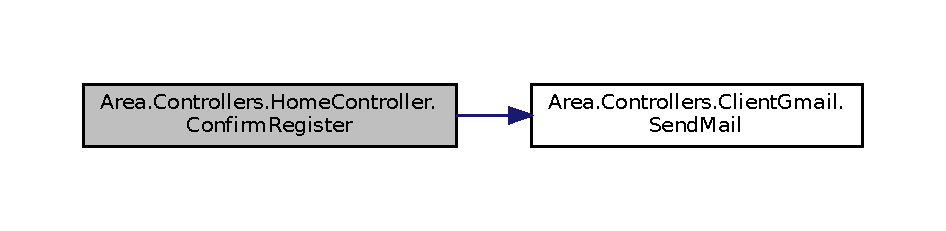
\includegraphics[width=350pt]{classArea_1_1Controllers_1_1HomeController_a510df0d8145d5ffcf8e89369b86e478c_cgraph}
\end{center}
\end{figure}
\mbox{\Hypertarget{classArea_1_1Controllers_1_1HomeController_a5e8c1711863dc28e3ec574f69aab79c5}\label{classArea_1_1Controllers_1_1HomeController_a5e8c1711863dc28e3ec574f69aab79c5}} 
\index{Area\+::\+Controllers\+::\+Home\+Controller@{Area\+::\+Controllers\+::\+Home\+Controller}!Confirm\+Register@{Confirm\+Register}}
\index{Confirm\+Register@{Confirm\+Register}!Area\+::\+Controllers\+::\+Home\+Controller@{Area\+::\+Controllers\+::\+Home\+Controller}}
\subsubsection{\texorpdfstring{Confirm\+Register()}{ConfirmRegister()}\hspace{0.1cm}{\footnotesize\ttfamily [2/2]}}
{\footnotesize\ttfamily I\+Action\+Result Area.\+Controllers.\+Home\+Controller.\+Confirm\+Register (\begin{DoxyParamCaption}\item[{\mbox{[}\+From\+Services\mbox{]} \mbox{\hyperlink{classArea_1_1DAT_1_1AreaDbContext}{Area\+Db\+Context}}}]{DB,  }\item[{\mbox{\hyperlink{classArea_1_1Models_1_1FormCode}{Form\+Code}}}]{model }\end{DoxyParamCaption})\hspace{0.3cm}{\ttfamily [inline]}}

\mbox{\Hypertarget{classArea_1_1Controllers_1_1HomeController_a029ed46ea5f2e8c9481d9c20f38b7875}\label{classArea_1_1Controllers_1_1HomeController_a029ed46ea5f2e8c9481d9c20f38b7875}} 
\index{Area\+::\+Controllers\+::\+Home\+Controller@{Area\+::\+Controllers\+::\+Home\+Controller}!Contact@{Contact}}
\index{Contact@{Contact}!Area\+::\+Controllers\+::\+Home\+Controller@{Area\+::\+Controllers\+::\+Home\+Controller}}
\subsubsection{\texorpdfstring{Contact()}{Contact()}}
{\footnotesize\ttfamily I\+Action\+Result Area.\+Controllers.\+Home\+Controller.\+Contact (\begin{DoxyParamCaption}\item[{\mbox{[}\+From\+Services\mbox{]} \mbox{\hyperlink{classArea_1_1DAT_1_1AreaDbContext}{Area\+Db\+Context}}}]{DB }\end{DoxyParamCaption})\hspace{0.3cm}{\ttfamily [inline]}}

\mbox{\Hypertarget{classArea_1_1Controllers_1_1HomeController_a99eb071c86613ccfe8003b803bceaafe}\label{classArea_1_1Controllers_1_1HomeController_a99eb071c86613ccfe8003b803bceaafe}} 
\index{Area\+::\+Controllers\+::\+Home\+Controller@{Area\+::\+Controllers\+::\+Home\+Controller}!Disconnect@{Disconnect}}
\index{Disconnect@{Disconnect}!Area\+::\+Controllers\+::\+Home\+Controller@{Area\+::\+Controllers\+::\+Home\+Controller}}
\subsubsection{\texorpdfstring{Disconnect()}{Disconnect()}}
{\footnotesize\ttfamily I\+Action\+Result Area.\+Controllers.\+Home\+Controller.\+Disconnect (\begin{DoxyParamCaption}\item[{\mbox{[}\+From\+Services\mbox{]} \mbox{\hyperlink{classArea_1_1DAT_1_1AreaDbContext}{Area\+Db\+Context}}}]{db\+Context }\end{DoxyParamCaption})\hspace{0.3cm}{\ttfamily [inline]}}

\mbox{\Hypertarget{classArea_1_1Controllers_1_1HomeController_a5770addb80c3fbaf23c159086b4c13d4}\label{classArea_1_1Controllers_1_1HomeController_a5770addb80c3fbaf23c159086b4c13d4}} 
\index{Area\+::\+Controllers\+::\+Home\+Controller@{Area\+::\+Controllers\+::\+Home\+Controller}!Error@{Error}}
\index{Error@{Error}!Area\+::\+Controllers\+::\+Home\+Controller@{Area\+::\+Controllers\+::\+Home\+Controller}}
\subsubsection{\texorpdfstring{Error()}{Error()}}
{\footnotesize\ttfamily I\+Action\+Result Area.\+Controllers.\+Home\+Controller.\+Error (\begin{DoxyParamCaption}{ }\end{DoxyParamCaption})\hspace{0.3cm}{\ttfamily [inline]}}

\mbox{\Hypertarget{classArea_1_1Controllers_1_1HomeController_a81852c6564831c3ba0cf7eddfc354997}\label{classArea_1_1Controllers_1_1HomeController_a81852c6564831c3ba0cf7eddfc354997}} 
\index{Area\+::\+Controllers\+::\+Home\+Controller@{Area\+::\+Controllers\+::\+Home\+Controller}!Index@{Index}}
\index{Index@{Index}!Area\+::\+Controllers\+::\+Home\+Controller@{Area\+::\+Controllers\+::\+Home\+Controller}}
\subsubsection{\texorpdfstring{Index()}{Index()}}
{\footnotesize\ttfamily I\+Action\+Result Area.\+Controllers.\+Home\+Controller.\+Index (\begin{DoxyParamCaption}\item[{\mbox{[}\+From\+Services\mbox{]} \mbox{\hyperlink{classArea_1_1DAT_1_1AreaDbContext}{Area\+Db\+Context}}}]{DB }\end{DoxyParamCaption})\hspace{0.3cm}{\ttfamily [inline]}}

\mbox{\Hypertarget{classArea_1_1Controllers_1_1HomeController_a41a57542642ed1c4b052975954a0794b}\label{classArea_1_1Controllers_1_1HomeController_a41a57542642ed1c4b052975954a0794b}} 
\index{Area\+::\+Controllers\+::\+Home\+Controller@{Area\+::\+Controllers\+::\+Home\+Controller}!Is\+Log@{Is\+Log}}
\index{Is\+Log@{Is\+Log}!Area\+::\+Controllers\+::\+Home\+Controller@{Area\+::\+Controllers\+::\+Home\+Controller}}
\subsubsection{\texorpdfstring{Is\+Log()}{IsLog()}}
{\footnotesize\ttfamily bool Area.\+Controllers.\+Home\+Controller.\+Is\+Log (\begin{DoxyParamCaption}\item[{\mbox{[}\+From\+Services\mbox{]} \mbox{\hyperlink{classArea_1_1DAT_1_1AreaDbContext}{Area\+Db\+Context}}}]{DB }\end{DoxyParamCaption})\hspace{0.3cm}{\ttfamily [inline]}, {\ttfamily [private]}}

\mbox{\Hypertarget{classArea_1_1Controllers_1_1HomeController_a5e4cf8ba8004592c197e31621233ff79}\label{classArea_1_1Controllers_1_1HomeController_a5e4cf8ba8004592c197e31621233ff79}} 
\index{Area\+::\+Controllers\+::\+Home\+Controller@{Area\+::\+Controllers\+::\+Home\+Controller}!Login@{Login}}
\index{Login@{Login}!Area\+::\+Controllers\+::\+Home\+Controller@{Area\+::\+Controllers\+::\+Home\+Controller}}
\subsubsection{\texorpdfstring{Login()}{Login()}\hspace{0.1cm}{\footnotesize\ttfamily [1/2]}}
{\footnotesize\ttfamily I\+Action\+Result Area.\+Controllers.\+Home\+Controller.\+Login (\begin{DoxyParamCaption}\item[{\mbox{[}\+From\+Services\mbox{]} \mbox{\hyperlink{classArea_1_1DAT_1_1AreaDbContext}{Area\+Db\+Context}}}]{DB }\end{DoxyParamCaption})\hspace{0.3cm}{\ttfamily [inline]}}

\mbox{\Hypertarget{classArea_1_1Controllers_1_1HomeController_a998f5002ebee5cf5ae63d206b816cd8c}\label{classArea_1_1Controllers_1_1HomeController_a998f5002ebee5cf5ae63d206b816cd8c}} 
\index{Area\+::\+Controllers\+::\+Home\+Controller@{Area\+::\+Controllers\+::\+Home\+Controller}!Login@{Login}}
\index{Login@{Login}!Area\+::\+Controllers\+::\+Home\+Controller@{Area\+::\+Controllers\+::\+Home\+Controller}}
\subsubsection{\texorpdfstring{Login()}{Login()}\hspace{0.1cm}{\footnotesize\ttfamily [2/2]}}
{\footnotesize\ttfamily I\+Action\+Result Area.\+Controllers.\+Home\+Controller.\+Login (\begin{DoxyParamCaption}\item[{\mbox{[}\+From\+Services\mbox{]} \mbox{\hyperlink{classArea_1_1DAT_1_1AreaDbContext}{Area\+Db\+Context}}}]{DB,  }\item[{\mbox{\hyperlink{classArea_1_1Models_1_1FormLogin}{Form\+Login}}}]{model }\end{DoxyParamCaption})\hspace{0.3cm}{\ttfamily [inline]}}

\mbox{\Hypertarget{classArea_1_1Controllers_1_1HomeController_a31ceb7fc34f6e2dec98d5b4e5989d3c7}\label{classArea_1_1Controllers_1_1HomeController_a31ceb7fc34f6e2dec98d5b4e5989d3c7}} 
\index{Area\+::\+Controllers\+::\+Home\+Controller@{Area\+::\+Controllers\+::\+Home\+Controller}!Manage\+Area@{Manage\+Area}}
\index{Manage\+Area@{Manage\+Area}!Area\+::\+Controllers\+::\+Home\+Controller@{Area\+::\+Controllers\+::\+Home\+Controller}}
\subsubsection{\texorpdfstring{Manage\+Area()}{ManageArea()}}
{\footnotesize\ttfamily I\+Action\+Result Area.\+Controllers.\+Home\+Controller.\+Manage\+Area (\begin{DoxyParamCaption}\item[{\mbox{[}\+From\+Services\mbox{]} \mbox{\hyperlink{classArea_1_1DAT_1_1AreaDbContext}{Area\+Db\+Context}}}]{DB }\end{DoxyParamCaption})\hspace{0.3cm}{\ttfamily [inline]}}

\mbox{\Hypertarget{classArea_1_1Controllers_1_1HomeController_a3ed060342c26dee6645dfc7bc0204f09}\label{classArea_1_1Controllers_1_1HomeController_a3ed060342c26dee6645dfc7bc0204f09}} 
\index{Area\+::\+Controllers\+::\+Home\+Controller@{Area\+::\+Controllers\+::\+Home\+Controller}!Register@{Register}}
\index{Register@{Register}!Area\+::\+Controllers\+::\+Home\+Controller@{Area\+::\+Controllers\+::\+Home\+Controller}}
\subsubsection{\texorpdfstring{Register()}{Register()}\hspace{0.1cm}{\footnotesize\ttfamily [1/2]}}
{\footnotesize\ttfamily I\+Action\+Result Area.\+Controllers.\+Home\+Controller.\+Register (\begin{DoxyParamCaption}\item[{\mbox{[}\+From\+Services\mbox{]} \mbox{\hyperlink{classArea_1_1DAT_1_1AreaDbContext}{Area\+Db\+Context}}}]{DB }\end{DoxyParamCaption})\hspace{0.3cm}{\ttfamily [inline]}}

\mbox{\Hypertarget{classArea_1_1Controllers_1_1HomeController_a3062b0baba8394d263dca4bb3a19427a}\label{classArea_1_1Controllers_1_1HomeController_a3062b0baba8394d263dca4bb3a19427a}} 
\index{Area\+::\+Controllers\+::\+Home\+Controller@{Area\+::\+Controllers\+::\+Home\+Controller}!Register@{Register}}
\index{Register@{Register}!Area\+::\+Controllers\+::\+Home\+Controller@{Area\+::\+Controllers\+::\+Home\+Controller}}
\subsubsection{\texorpdfstring{Register()}{Register()}\hspace{0.1cm}{\footnotesize\ttfamily [2/2]}}
{\footnotesize\ttfamily I\+Action\+Result Area.\+Controllers.\+Home\+Controller.\+Register (\begin{DoxyParamCaption}\item[{\mbox{[}\+From\+Services\mbox{]} \mbox{\hyperlink{classArea_1_1DAT_1_1AreaDbContext}{Area\+Db\+Context}}}]{DB,  }\item[{\mbox{\hyperlink{classArea_1_1Models_1_1FormRegister}{Form\+Register}}}]{model }\end{DoxyParamCaption})\hspace{0.3cm}{\ttfamily [inline]}}



The documentation for this class was generated from the following file\+:\begin{DoxyCompactItemize}
\item 
Controllers/\mbox{\hyperlink{HomeController_8cs}{Home\+Controller.\+cs}}\end{DoxyCompactItemize}

\hypertarget{interfaceArea_1_1Models_1_1IArea}{}\section{Area.\+Models.\+I\+Area Interface Reference}
\label{interfaceArea_1_1Models_1_1IArea}\index{Area.\+Models.\+I\+Area@{Area.\+Models.\+I\+Area}}


Inheritance diagram for Area.\+Models.\+I\+Area\+:
\nopagebreak
\begin{figure}[H]
\begin{center}
\leavevmode
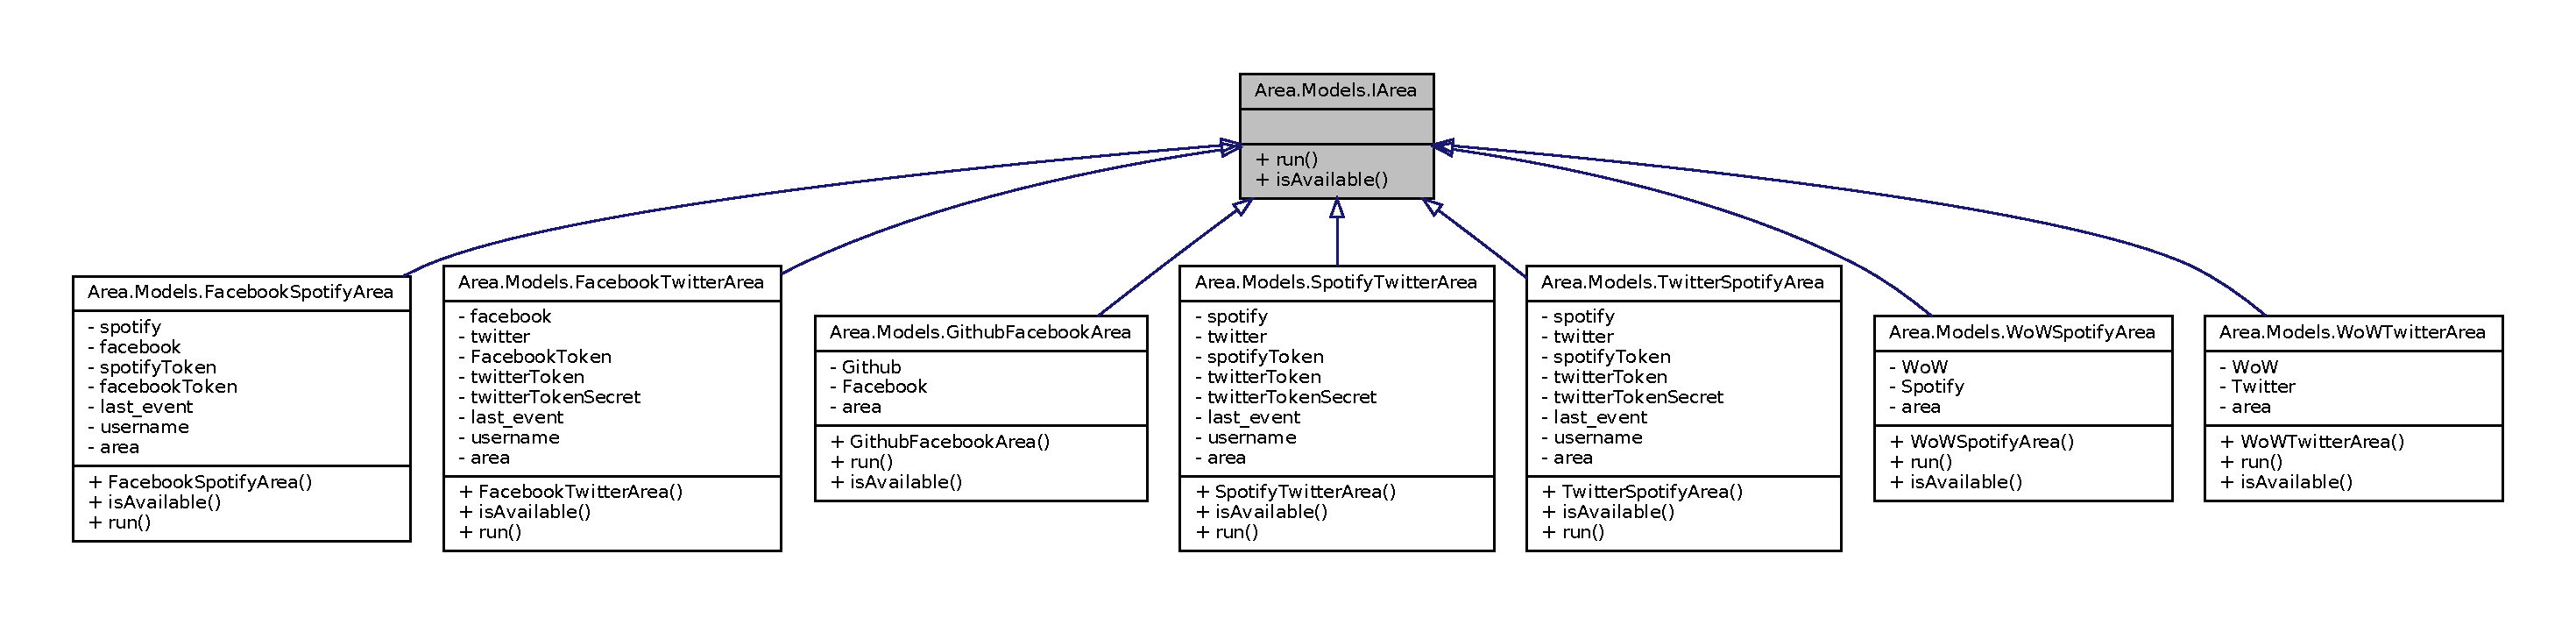
\includegraphics[width=350pt]{interfaceArea_1_1Models_1_1IArea__inherit__graph}
\end{center}
\end{figure}


Collaboration diagram for Area.\+Models.\+I\+Area\+:
\nopagebreak
\begin{figure}[H]
\begin{center}
\leavevmode
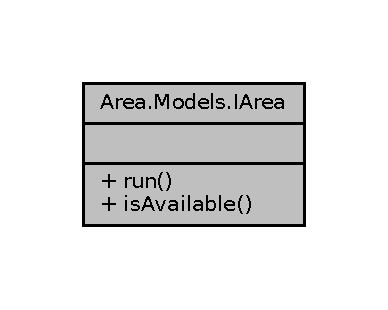
\includegraphics[width=186pt]{interfaceArea_1_1Models_1_1IArea__coll__graph}
\end{center}
\end{figure}
\subsection*{Public Member Functions}
\begin{DoxyCompactItemize}
\item 
void \mbox{\hyperlink{interfaceArea_1_1Models_1_1IArea_af153822d2715dad8eb1c250bcc4de567}{run}} (\mbox{\hyperlink{classArea_1_1DAT_1_1AreaDbContext}{Area\+Db\+Context}} DB)
\item 
bool \mbox{\hyperlink{interfaceArea_1_1Models_1_1IArea_a742b324f0d7573f7f99f9e2adb5df94c}{is\+Available}} ()
\end{DoxyCompactItemize}


\subsection{Member Function Documentation}
\mbox{\Hypertarget{interfaceArea_1_1Models_1_1IArea_a742b324f0d7573f7f99f9e2adb5df94c}\label{interfaceArea_1_1Models_1_1IArea_a742b324f0d7573f7f99f9e2adb5df94c}} 
\index{Area\+::\+Models\+::\+I\+Area@{Area\+::\+Models\+::\+I\+Area}!is\+Available@{is\+Available}}
\index{is\+Available@{is\+Available}!Area\+::\+Models\+::\+I\+Area@{Area\+::\+Models\+::\+I\+Area}}
\subsubsection{\texorpdfstring{is\+Available()}{isAvailable()}}
{\footnotesize\ttfamily bool Area.\+Models.\+I\+Area.\+is\+Available (\begin{DoxyParamCaption}{ }\end{DoxyParamCaption})}



Implemented in \mbox{\hyperlink{classArea_1_1Models_1_1WoWTwitterArea_af69bc0b27a27e86935da99d750d80f17}{Area.\+Models.\+Wo\+W\+Twitter\+Area}}, \mbox{\hyperlink{classArea_1_1Models_1_1WoWSpotifyArea_a577046acb0b4537ab57367893dfee2c0}{Area.\+Models.\+Wo\+W\+Spotify\+Area}}, \mbox{\hyperlink{classArea_1_1Models_1_1GithubFacebookArea_ab1f22cb94018e33fa92221c812da1020}{Area.\+Models.\+Github\+Facebook\+Area}}, \mbox{\hyperlink{classArea_1_1Models_1_1FacebookTwitterArea_a654f1444c68fdbeb379c6df404b5b9f9}{Area.\+Models.\+Facebook\+Twitter\+Area}}, \mbox{\hyperlink{classArea_1_1Models_1_1SpotifyTwitterArea_a087443bd0237323d56e02286868b0345}{Area.\+Models.\+Spotify\+Twitter\+Area}}, \mbox{\hyperlink{classArea_1_1Models_1_1TwitterSpotifyArea_a0a58941ea11c4ec34da9319efc4eb6d3}{Area.\+Models.\+Twitter\+Spotify\+Area}}, and \mbox{\hyperlink{classArea_1_1Models_1_1FacebookSpotifyArea_aa98a5f78b4814107265c952496c50fcb}{Area.\+Models.\+Facebook\+Spotify\+Area}}.

\mbox{\Hypertarget{interfaceArea_1_1Models_1_1IArea_af153822d2715dad8eb1c250bcc4de567}\label{interfaceArea_1_1Models_1_1IArea_af153822d2715dad8eb1c250bcc4de567}} 
\index{Area\+::\+Models\+::\+I\+Area@{Area\+::\+Models\+::\+I\+Area}!run@{run}}
\index{run@{run}!Area\+::\+Models\+::\+I\+Area@{Area\+::\+Models\+::\+I\+Area}}
\subsubsection{\texorpdfstring{run()}{run()}}
{\footnotesize\ttfamily void Area.\+Models.\+I\+Area.\+run (\begin{DoxyParamCaption}\item[{\mbox{\hyperlink{classArea_1_1DAT_1_1AreaDbContext}{Area\+Db\+Context}}}]{DB }\end{DoxyParamCaption})}



Implemented in \mbox{\hyperlink{classArea_1_1Models_1_1FacebookTwitterArea_a6fd52c3124301206f73b8c9f025872d4}{Area.\+Models.\+Facebook\+Twitter\+Area}}, \mbox{\hyperlink{classArea_1_1Models_1_1SpotifyTwitterArea_ada41191b6c76e9be5677b1e4e175ea23}{Area.\+Models.\+Spotify\+Twitter\+Area}}, \mbox{\hyperlink{classArea_1_1Models_1_1TwitterSpotifyArea_a6ff9d29fc453210f86a59959c89848c4}{Area.\+Models.\+Twitter\+Spotify\+Area}}, \mbox{\hyperlink{classArea_1_1Models_1_1FacebookSpotifyArea_ae574aa239311b4fc84d087adef335f3d}{Area.\+Models.\+Facebook\+Spotify\+Area}}, \mbox{\hyperlink{classArea_1_1Models_1_1WoWTwitterArea_a56856ed9dc553111f0c5db1a4813f565}{Area.\+Models.\+Wo\+W\+Twitter\+Area}}, \mbox{\hyperlink{classArea_1_1Models_1_1WoWSpotifyArea_a2920b3707f791839a3ec17d9ab45f3df}{Area.\+Models.\+Wo\+W\+Spotify\+Area}}, and \mbox{\hyperlink{classArea_1_1Models_1_1GithubFacebookArea_a984d46335dd21d81088312ebe413a0fc}{Area.\+Models.\+Github\+Facebook\+Area}}.



The documentation for this interface was generated from the following file\+:\begin{DoxyCompactItemize}
\item 
Models/\+Areas/\mbox{\hyperlink{IArea_8cs}{I\+Area.\+cs}}\end{DoxyCompactItemize}

\hypertarget{interfaceArea_1_1Models_1_1IModuleModel}{}\section{Area.\+Models.\+I\+Module\+Model Interface Reference}
\label{interfaceArea_1_1Models_1_1IModuleModel}\index{Area.\+Models.\+I\+Module\+Model@{Area.\+Models.\+I\+Module\+Model}}


Inheritance diagram for Area.\+Models.\+I\+Module\+Model\+:
\nopagebreak
\begin{figure}[H]
\begin{center}
\leavevmode
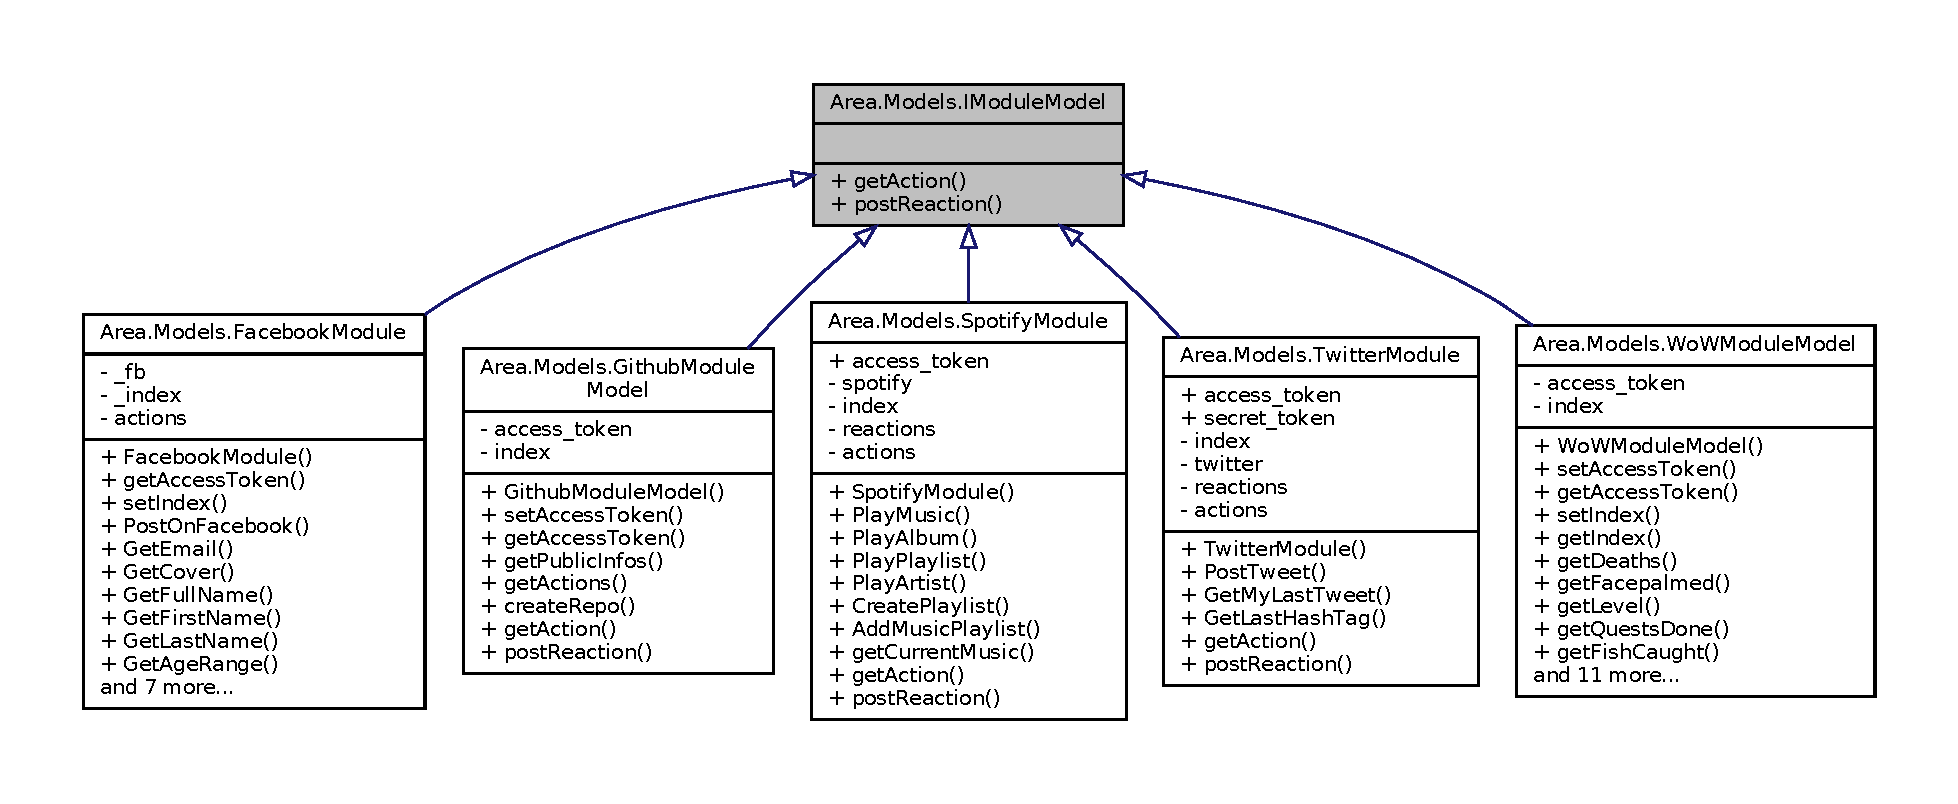
\includegraphics[width=350pt]{interfaceArea_1_1Models_1_1IModuleModel__inherit__graph}
\end{center}
\end{figure}


Collaboration diagram for Area.\+Models.\+I\+Module\+Model\+:
\nopagebreak
\begin{figure}[H]
\begin{center}
\leavevmode
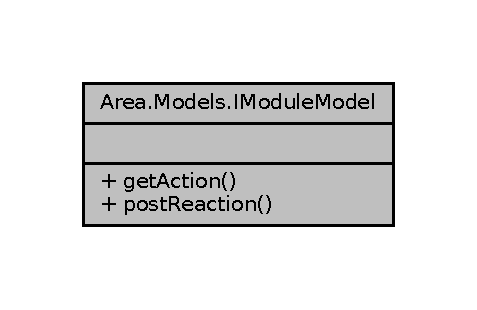
\includegraphics[width=229pt]{interfaceArea_1_1Models_1_1IModuleModel__coll__graph}
\end{center}
\end{figure}
\subsection*{Public Member Functions}
\begin{DoxyCompactItemize}
\item 
string \mbox{\hyperlink{interfaceArea_1_1Models_1_1IModuleModel_a050d892fae9f85c6b607a7c0e30502e9}{get\+Action}} ()
\item 
void \mbox{\hyperlink{interfaceArea_1_1Models_1_1IModuleModel_af2c1a82bd894255ab2099440f4f3d6f7}{post\+Reaction}} (string reaction)
\end{DoxyCompactItemize}


\subsection{Member Function Documentation}
\mbox{\Hypertarget{interfaceArea_1_1Models_1_1IModuleModel_a050d892fae9f85c6b607a7c0e30502e9}\label{interfaceArea_1_1Models_1_1IModuleModel_a050d892fae9f85c6b607a7c0e30502e9}} 
\index{Area\+::\+Models\+::\+I\+Module\+Model@{Area\+::\+Models\+::\+I\+Module\+Model}!get\+Action@{get\+Action}}
\index{get\+Action@{get\+Action}!Area\+::\+Models\+::\+I\+Module\+Model@{Area\+::\+Models\+::\+I\+Module\+Model}}
\subsubsection{\texorpdfstring{get\+Action()}{getAction()}}
{\footnotesize\ttfamily string Area.\+Models.\+I\+Module\+Model.\+get\+Action (\begin{DoxyParamCaption}{ }\end{DoxyParamCaption})}



Implemented in \mbox{\hyperlink{classArea_1_1Models_1_1FacebookModule_aeb88d4de280aa76fa80c92509b7df265}{Area.\+Models.\+Facebook\+Module}}, \mbox{\hyperlink{classArea_1_1Models_1_1WoWModuleModel_a3ed39b2aeec20f1d908d9c6e43aad389}{Area.\+Models.\+Wo\+W\+Module\+Model}}, \mbox{\hyperlink{classArea_1_1Models_1_1SpotifyModule_ad506554a80eb35db2d6d9c251f38a5b7}{Area.\+Models.\+Spotify\+Module}}, \mbox{\hyperlink{classArea_1_1Models_1_1GithubModuleModel_aebec4ccbd02441daa062ce936a9f4e3d}{Area.\+Models.\+Github\+Module\+Model}}, and \mbox{\hyperlink{classArea_1_1Models_1_1TwitterModule_a80551107a68f78bf23d57948dcbe5a6d}{Area.\+Models.\+Twitter\+Module}}.

\mbox{\Hypertarget{interfaceArea_1_1Models_1_1IModuleModel_af2c1a82bd894255ab2099440f4f3d6f7}\label{interfaceArea_1_1Models_1_1IModuleModel_af2c1a82bd894255ab2099440f4f3d6f7}} 
\index{Area\+::\+Models\+::\+I\+Module\+Model@{Area\+::\+Models\+::\+I\+Module\+Model}!post\+Reaction@{post\+Reaction}}
\index{post\+Reaction@{post\+Reaction}!Area\+::\+Models\+::\+I\+Module\+Model@{Area\+::\+Models\+::\+I\+Module\+Model}}
\subsubsection{\texorpdfstring{post\+Reaction()}{postReaction()}}
{\footnotesize\ttfamily void Area.\+Models.\+I\+Module\+Model.\+post\+Reaction (\begin{DoxyParamCaption}\item[{string}]{reaction }\end{DoxyParamCaption})}



Implemented in \mbox{\hyperlink{classArea_1_1Models_1_1FacebookModule_aa992d24aaa0e9ebd0a2f2c38607222d5}{Area.\+Models.\+Facebook\+Module}}, \mbox{\hyperlink{classArea_1_1Models_1_1WoWModuleModel_a04335d82b02dd3cfe3b9ae0cb47125f6}{Area.\+Models.\+Wo\+W\+Module\+Model}}, \mbox{\hyperlink{classArea_1_1Models_1_1SpotifyModule_a54a02b412af1c23ffa05f0bc9c7bd228}{Area.\+Models.\+Spotify\+Module}}, \mbox{\hyperlink{classArea_1_1Models_1_1GithubModuleModel_aeeda0ad6ec3b9ddaa5a38e9b8a2ef020}{Area.\+Models.\+Github\+Module\+Model}}, and \mbox{\hyperlink{classArea_1_1Models_1_1TwitterModule_a2dd56c4273c09ea000d0229bb9d19019}{Area.\+Models.\+Twitter\+Module}}.



The documentation for this interface was generated from the following file\+:\begin{DoxyCompactItemize}
\item 
Models/\+Modules/\mbox{\hyperlink{IModuleModel_8cs}{I\+Module\+Model.\+cs}}\end{DoxyCompactItemize}

\hypertarget{classArea_1_1Controllers_1_1ManageAreaController}{}\section{Area.\+Controllers.\+Manage\+Area\+Controller Class Reference}
\label{classArea_1_1Controllers_1_1ManageAreaController}\index{Area.\+Controllers.\+Manage\+Area\+Controller@{Area.\+Controllers.\+Manage\+Area\+Controller}}


Inheritance diagram for Area.\+Controllers.\+Manage\+Area\+Controller\+:
\nopagebreak
\begin{figure}[H]
\begin{center}
\leavevmode
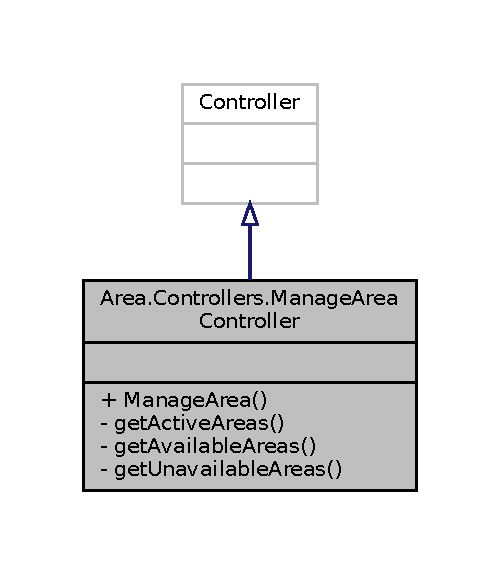
\includegraphics[width=240pt]{classArea_1_1Controllers_1_1ManageAreaController__inherit__graph}
\end{center}
\end{figure}


Collaboration diagram for Area.\+Controllers.\+Manage\+Area\+Controller\+:
\nopagebreak
\begin{figure}[H]
\begin{center}
\leavevmode
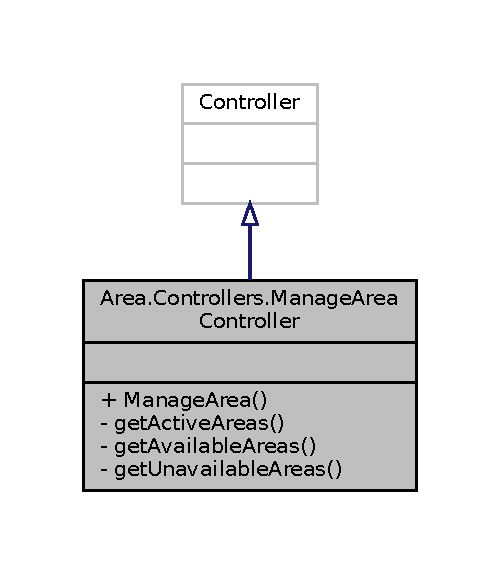
\includegraphics[width=240pt]{classArea_1_1Controllers_1_1ManageAreaController__coll__graph}
\end{center}
\end{figure}
\subsection*{Public Member Functions}
\begin{DoxyCompactItemize}
\item 
Action\+Result \mbox{\hyperlink{classArea_1_1Controllers_1_1ManageAreaController_a5d3d86fcfe1e256e1ca8f8f316f5a9fc}{Manage\+Area}} (\mbox{[}From\+Services\mbox{]} \mbox{\hyperlink{classArea_1_1DAT_1_1AreaDbContext}{Area\+Db\+Context}} DB)
\end{DoxyCompactItemize}
\subsection*{Private Member Functions}
\begin{DoxyCompactItemize}
\item 
List$<$ \mbox{\hyperlink{classArea_1_1Models_1_1AreaType}{Area\+Type}} $>$ \mbox{\hyperlink{classArea_1_1Controllers_1_1ManageAreaController_af30cf6d59cf0ce70de54adc3f706da0b}{get\+Active\+Areas}} (\mbox{\hyperlink{classArea_1_1DAT_1_1AreaDbContext}{Area\+Db\+Context}} DB, string username)
\item 
List$<$ \mbox{\hyperlink{classArea_1_1Models_1_1AreaType}{Area\+Type}} $>$ \mbox{\hyperlink{classArea_1_1Controllers_1_1ManageAreaController_a04c1155798ffbfc4f87564fe48db8981}{get\+Available\+Areas}} (\mbox{\hyperlink{classArea_1_1DAT_1_1AreaDbContext}{Area\+Db\+Context}} DB, string username)
\item 
List$<$ \mbox{\hyperlink{classArea_1_1Models_1_1AreaType}{Area\+Type}} $>$ \mbox{\hyperlink{classArea_1_1Controllers_1_1ManageAreaController_a17a1989e93097ab54cf340bbfafd7bb3}{get\+Unavailable\+Areas}} (\mbox{\hyperlink{classArea_1_1DAT_1_1AreaDbContext}{Area\+Db\+Context}} DB, string username)
\end{DoxyCompactItemize}


\subsection{Member Function Documentation}
\mbox{\Hypertarget{classArea_1_1Controllers_1_1ManageAreaController_af30cf6d59cf0ce70de54adc3f706da0b}\label{classArea_1_1Controllers_1_1ManageAreaController_af30cf6d59cf0ce70de54adc3f706da0b}} 
\index{Area\+::\+Controllers\+::\+Manage\+Area\+Controller@{Area\+::\+Controllers\+::\+Manage\+Area\+Controller}!get\+Active\+Areas@{get\+Active\+Areas}}
\index{get\+Active\+Areas@{get\+Active\+Areas}!Area\+::\+Controllers\+::\+Manage\+Area\+Controller@{Area\+::\+Controllers\+::\+Manage\+Area\+Controller}}
\subsubsection{\texorpdfstring{get\+Active\+Areas()}{getActiveAreas()}}
{\footnotesize\ttfamily List$<$\mbox{\hyperlink{classArea_1_1Models_1_1AreaType}{Area\+Type}}$>$ Area.\+Controllers.\+Manage\+Area\+Controller.\+get\+Active\+Areas (\begin{DoxyParamCaption}\item[{\mbox{\hyperlink{classArea_1_1DAT_1_1AreaDbContext}{Area\+Db\+Context}}}]{DB,  }\item[{string}]{username }\end{DoxyParamCaption})\hspace{0.3cm}{\ttfamily [inline]}, {\ttfamily [private]}}

Here is the call graph for this function\+:
\nopagebreak
\begin{figure}[H]
\begin{center}
\leavevmode
\includegraphics[width=350pt]{classArea_1_1Controllers_1_1ManageAreaController_af30cf6d59cf0ce70de54adc3f706da0b_cgraph}
\end{center}
\end{figure}
\mbox{\Hypertarget{classArea_1_1Controllers_1_1ManageAreaController_a04c1155798ffbfc4f87564fe48db8981}\label{classArea_1_1Controllers_1_1ManageAreaController_a04c1155798ffbfc4f87564fe48db8981}} 
\index{Area\+::\+Controllers\+::\+Manage\+Area\+Controller@{Area\+::\+Controllers\+::\+Manage\+Area\+Controller}!get\+Available\+Areas@{get\+Available\+Areas}}
\index{get\+Available\+Areas@{get\+Available\+Areas}!Area\+::\+Controllers\+::\+Manage\+Area\+Controller@{Area\+::\+Controllers\+::\+Manage\+Area\+Controller}}
\subsubsection{\texorpdfstring{get\+Available\+Areas()}{getAvailableAreas()}}
{\footnotesize\ttfamily List$<$\mbox{\hyperlink{classArea_1_1Models_1_1AreaType}{Area\+Type}}$>$ Area.\+Controllers.\+Manage\+Area\+Controller.\+get\+Available\+Areas (\begin{DoxyParamCaption}\item[{\mbox{\hyperlink{classArea_1_1DAT_1_1AreaDbContext}{Area\+Db\+Context}}}]{DB,  }\item[{string}]{username }\end{DoxyParamCaption})\hspace{0.3cm}{\ttfamily [inline]}, {\ttfamily [private]}}

Here is the call graph for this function\+:
\nopagebreak
\begin{figure}[H]
\begin{center}
\leavevmode
\includegraphics[width=350pt]{classArea_1_1Controllers_1_1ManageAreaController_a04c1155798ffbfc4f87564fe48db8981_cgraph}
\end{center}
\end{figure}
\mbox{\Hypertarget{classArea_1_1Controllers_1_1ManageAreaController_a17a1989e93097ab54cf340bbfafd7bb3}\label{classArea_1_1Controllers_1_1ManageAreaController_a17a1989e93097ab54cf340bbfafd7bb3}} 
\index{Area\+::\+Controllers\+::\+Manage\+Area\+Controller@{Area\+::\+Controllers\+::\+Manage\+Area\+Controller}!get\+Unavailable\+Areas@{get\+Unavailable\+Areas}}
\index{get\+Unavailable\+Areas@{get\+Unavailable\+Areas}!Area\+::\+Controllers\+::\+Manage\+Area\+Controller@{Area\+::\+Controllers\+::\+Manage\+Area\+Controller}}
\subsubsection{\texorpdfstring{get\+Unavailable\+Areas()}{getUnavailableAreas()}}
{\footnotesize\ttfamily List$<$\mbox{\hyperlink{classArea_1_1Models_1_1AreaType}{Area\+Type}}$>$ Area.\+Controllers.\+Manage\+Area\+Controller.\+get\+Unavailable\+Areas (\begin{DoxyParamCaption}\item[{\mbox{\hyperlink{classArea_1_1DAT_1_1AreaDbContext}{Area\+Db\+Context}}}]{DB,  }\item[{string}]{username }\end{DoxyParamCaption})\hspace{0.3cm}{\ttfamily [inline]}, {\ttfamily [private]}}

Here is the call graph for this function\+:
\nopagebreak
\begin{figure}[H]
\begin{center}
\leavevmode
\includegraphics[width=350pt]{classArea_1_1Controllers_1_1ManageAreaController_a17a1989e93097ab54cf340bbfafd7bb3_cgraph}
\end{center}
\end{figure}
\mbox{\Hypertarget{classArea_1_1Controllers_1_1ManageAreaController_a5d3d86fcfe1e256e1ca8f8f316f5a9fc}\label{classArea_1_1Controllers_1_1ManageAreaController_a5d3d86fcfe1e256e1ca8f8f316f5a9fc}} 
\index{Area\+::\+Controllers\+::\+Manage\+Area\+Controller@{Area\+::\+Controllers\+::\+Manage\+Area\+Controller}!Manage\+Area@{Manage\+Area}}
\index{Manage\+Area@{Manage\+Area}!Area\+::\+Controllers\+::\+Manage\+Area\+Controller@{Area\+::\+Controllers\+::\+Manage\+Area\+Controller}}
\subsubsection{\texorpdfstring{Manage\+Area()}{ManageArea()}}
{\footnotesize\ttfamily Action\+Result Area.\+Controllers.\+Manage\+Area\+Controller.\+Manage\+Area (\begin{DoxyParamCaption}\item[{\mbox{[}\+From\+Services\mbox{]} \mbox{\hyperlink{classArea_1_1DAT_1_1AreaDbContext}{Area\+Db\+Context}}}]{DB }\end{DoxyParamCaption})\hspace{0.3cm}{\ttfamily [inline]}}



The documentation for this class was generated from the following file\+:\begin{DoxyCompactItemize}
\item 
Controllers/\mbox{\hyperlink{ManageAreaController_8cs}{Manage\+Area\+Controller.\+cs}}\end{DoxyCompactItemize}

\hypertarget{classArea_1_1Program}{}\section{Area.\+Program Class Reference}
\label{classArea_1_1Program}\index{Area.\+Program@{Area.\+Program}}


Collaboration diagram for Area.\+Program\+:
\nopagebreak
\begin{figure}[H]
\begin{center}
\leavevmode
\includegraphics[width=184pt]{classArea_1_1Program__coll__graph}
\end{center}
\end{figure}
\subsection*{Static Public Member Functions}
\begin{DoxyCompactItemize}
\item 
static void \mbox{\hyperlink{classArea_1_1Program_a3d170d98ebe8cc51ab2fcb4b23684264}{Main}} (string\mbox{[}$\,$\mbox{]} args)
\item 
static I\+Web\+Host \mbox{\hyperlink{classArea_1_1Program_a0a25fed84b06a0c02fa7c6dd334ebd0f}{Build\+Web\+Host}} (string\mbox{[}$\,$\mbox{]} args)
\end{DoxyCompactItemize}


\subsection{Member Function Documentation}
\mbox{\Hypertarget{classArea_1_1Program_a0a25fed84b06a0c02fa7c6dd334ebd0f}\label{classArea_1_1Program_a0a25fed84b06a0c02fa7c6dd334ebd0f}} 
\index{Area\+::\+Program@{Area\+::\+Program}!Build\+Web\+Host@{Build\+Web\+Host}}
\index{Build\+Web\+Host@{Build\+Web\+Host}!Area\+::\+Program@{Area\+::\+Program}}
\subsubsection{\texorpdfstring{Build\+Web\+Host()}{BuildWebHost()}}
{\footnotesize\ttfamily static I\+Web\+Host Area.\+Program.\+Build\+Web\+Host (\begin{DoxyParamCaption}\item[{string \mbox{[}$\,$\mbox{]}}]{args }\end{DoxyParamCaption})\hspace{0.3cm}{\ttfamily [static]}}

\mbox{\Hypertarget{classArea_1_1Program_a3d170d98ebe8cc51ab2fcb4b23684264}\label{classArea_1_1Program_a3d170d98ebe8cc51ab2fcb4b23684264}} 
\index{Area\+::\+Program@{Area\+::\+Program}!Main@{Main}}
\index{Main@{Main}!Area\+::\+Program@{Area\+::\+Program}}
\subsubsection{\texorpdfstring{Main()}{Main()}}
{\footnotesize\ttfamily static void Area.\+Program.\+Main (\begin{DoxyParamCaption}\item[{string \mbox{[}$\,$\mbox{]}}]{args }\end{DoxyParamCaption})\hspace{0.3cm}{\ttfamily [inline]}, {\ttfamily [static]}}

Here is the call graph for this function\+:
\nopagebreak
\begin{figure}[H]
\begin{center}
\leavevmode
\includegraphics[width=350pt]{classArea_1_1Program_a3d170d98ebe8cc51ab2fcb4b23684264_cgraph}
\end{center}
\end{figure}


The documentation for this class was generated from the following file\+:\begin{DoxyCompactItemize}
\item 
\mbox{\hyperlink{Program_8cs}{Program.\+cs}}\end{DoxyCompactItemize}

\hypertarget{classArea_1_1Controllers_1_1SpotifyController}{}\section{Area.\+Controllers.\+Spotify\+Controller Class Reference}
\label{classArea_1_1Controllers_1_1SpotifyController}\index{Area.\+Controllers.\+Spotify\+Controller@{Area.\+Controllers.\+Spotify\+Controller}}


Inheritance diagram for Area.\+Controllers.\+Spotify\+Controller\+:
\nopagebreak
\begin{figure}[H]
\begin{center}
\leavevmode
\includegraphics[width=213pt]{classArea_1_1Controllers_1_1SpotifyController__inherit__graph}
\end{center}
\end{figure}


Collaboration diagram for Area.\+Controllers.\+Spotify\+Controller\+:
\nopagebreak
\begin{figure}[H]
\begin{center}
\leavevmode
\includegraphics[width=213pt]{classArea_1_1Controllers_1_1SpotifyController__coll__graph}
\end{center}
\end{figure}
\subsection*{Public Member Functions}
\begin{DoxyCompactItemize}
\item 
Action\+Result \mbox{\hyperlink{classArea_1_1Controllers_1_1SpotifyController_ac6ab1164412f4ec9ad7a9ad58ff5dc4f}{Auth}} ()
\item 
string \mbox{\hyperlink{classArea_1_1Controllers_1_1SpotifyController_a7d88f1761fc5ea275a0ccce707e81289}{Get\+Auth\+Uri}} ()
\item 
Action\+Result \mbox{\hyperlink{classArea_1_1Controllers_1_1SpotifyController_a47e94b8071f1917dba3f62cd9e4e9601}{Auth\+Response}} ()
\item 
Action\+Result \mbox{\hyperlink{classArea_1_1Controllers_1_1SpotifyController_a168ce6acbbe7e20e27742781a39bce95}{Connected}} (string access\+\_\+token, string token\+\_\+type, string expires\+\_\+in, string state, \mbox{[}From\+Services\mbox{]} \mbox{\hyperlink{classArea_1_1DAT_1_1AreaDbContext}{Area\+Db\+Context}} DB)
\end{DoxyCompactItemize}


\subsection{Member Function Documentation}
\mbox{\Hypertarget{classArea_1_1Controllers_1_1SpotifyController_ac6ab1164412f4ec9ad7a9ad58ff5dc4f}\label{classArea_1_1Controllers_1_1SpotifyController_ac6ab1164412f4ec9ad7a9ad58ff5dc4f}} 
\index{Area\+::\+Controllers\+::\+Spotify\+Controller@{Area\+::\+Controllers\+::\+Spotify\+Controller}!Auth@{Auth}}
\index{Auth@{Auth}!Area\+::\+Controllers\+::\+Spotify\+Controller@{Area\+::\+Controllers\+::\+Spotify\+Controller}}
\subsubsection{\texorpdfstring{Auth()}{Auth()}}
{\footnotesize\ttfamily Action\+Result Area.\+Controllers.\+Spotify\+Controller.\+Auth (\begin{DoxyParamCaption}{ }\end{DoxyParamCaption})\hspace{0.3cm}{\ttfamily [inline]}}

\mbox{\Hypertarget{classArea_1_1Controllers_1_1SpotifyController_a47e94b8071f1917dba3f62cd9e4e9601}\label{classArea_1_1Controllers_1_1SpotifyController_a47e94b8071f1917dba3f62cd9e4e9601}} 
\index{Area\+::\+Controllers\+::\+Spotify\+Controller@{Area\+::\+Controllers\+::\+Spotify\+Controller}!Auth\+Response@{Auth\+Response}}
\index{Auth\+Response@{Auth\+Response}!Area\+::\+Controllers\+::\+Spotify\+Controller@{Area\+::\+Controllers\+::\+Spotify\+Controller}}
\subsubsection{\texorpdfstring{Auth\+Response()}{AuthResponse()}}
{\footnotesize\ttfamily Action\+Result Area.\+Controllers.\+Spotify\+Controller.\+Auth\+Response (\begin{DoxyParamCaption}{ }\end{DoxyParamCaption})\hspace{0.3cm}{\ttfamily [inline]}}

\mbox{\Hypertarget{classArea_1_1Controllers_1_1SpotifyController_a168ce6acbbe7e20e27742781a39bce95}\label{classArea_1_1Controllers_1_1SpotifyController_a168ce6acbbe7e20e27742781a39bce95}} 
\index{Area\+::\+Controllers\+::\+Spotify\+Controller@{Area\+::\+Controllers\+::\+Spotify\+Controller}!Connected@{Connected}}
\index{Connected@{Connected}!Area\+::\+Controllers\+::\+Spotify\+Controller@{Area\+::\+Controllers\+::\+Spotify\+Controller}}
\subsubsection{\texorpdfstring{Connected()}{Connected()}}
{\footnotesize\ttfamily Action\+Result Area.\+Controllers.\+Spotify\+Controller.\+Connected (\begin{DoxyParamCaption}\item[{string}]{access\+\_\+token,  }\item[{string}]{token\+\_\+type,  }\item[{string}]{expires\+\_\+in,  }\item[{string}]{state,  }\item[{\mbox{[}\+From\+Services\mbox{]} \mbox{\hyperlink{classArea_1_1DAT_1_1AreaDbContext}{Area\+Db\+Context}}}]{DB }\end{DoxyParamCaption})\hspace{0.3cm}{\ttfamily [inline]}}

Here is the call graph for this function\+:
\nopagebreak
\begin{figure}[H]
\begin{center}
\leavevmode
\includegraphics[width=350pt]{classArea_1_1Controllers_1_1SpotifyController_a168ce6acbbe7e20e27742781a39bce95_cgraph}
\end{center}
\end{figure}
\mbox{\Hypertarget{classArea_1_1Controllers_1_1SpotifyController_a7d88f1761fc5ea275a0ccce707e81289}\label{classArea_1_1Controllers_1_1SpotifyController_a7d88f1761fc5ea275a0ccce707e81289}} 
\index{Area\+::\+Controllers\+::\+Spotify\+Controller@{Area\+::\+Controllers\+::\+Spotify\+Controller}!Get\+Auth\+Uri@{Get\+Auth\+Uri}}
\index{Get\+Auth\+Uri@{Get\+Auth\+Uri}!Area\+::\+Controllers\+::\+Spotify\+Controller@{Area\+::\+Controllers\+::\+Spotify\+Controller}}
\subsubsection{\texorpdfstring{Get\+Auth\+Uri()}{GetAuthUri()}}
{\footnotesize\ttfamily string Area.\+Controllers.\+Spotify\+Controller.\+Get\+Auth\+Uri (\begin{DoxyParamCaption}{ }\end{DoxyParamCaption})\hspace{0.3cm}{\ttfamily [inline]}}



The documentation for this class was generated from the following file\+:\begin{DoxyCompactItemize}
\item 
Controllers/\mbox{\hyperlink{SpotifyController_8cs}{Spotify\+Controller.\+cs}}\end{DoxyCompactItemize}

\hypertarget{classArea_1_1Models_1_1SpotifyModule}{}\section{Area.\+Models.\+Spotify\+Module Class Reference}
\label{classArea_1_1Models_1_1SpotifyModule}\index{Area.\+Models.\+Spotify\+Module@{Area.\+Models.\+Spotify\+Module}}


Inheritance diagram for Area.\+Models.\+Spotify\+Module\+:
\nopagebreak
\begin{figure}[H]
\begin{center}
\leavevmode
\includegraphics[width=231pt]{classArea_1_1Models_1_1SpotifyModule__inherit__graph}
\end{center}
\end{figure}


Collaboration diagram for Area.\+Models.\+Spotify\+Module\+:
\nopagebreak
\begin{figure}[H]
\begin{center}
\leavevmode
\includegraphics[width=231pt]{classArea_1_1Models_1_1SpotifyModule__coll__graph}
\end{center}
\end{figure}
\subsection*{Public Member Functions}
\begin{DoxyCompactItemize}
\item 
\mbox{\hyperlink{classArea_1_1Models_1_1SpotifyModule_a8bf87195b9980a22f5183a05242cd18c}{Spotify\+Module}} (string \mbox{\hyperlink{classArea_1_1Models_1_1SpotifyModule_aff156c8f9328648cb5a505b7f98bc030}{access\+\_\+token}}, int \mbox{\hyperlink{classArea_1_1Models_1_1SpotifyModule_acef664652a467d8655e04497e88a7dc5}{index}})
\item 
void \mbox{\hyperlink{classArea_1_1Models_1_1SpotifyModule_aa47b97c81021848c70064a367c08805f}{Play\+Music}} (string name)
\item 
void \mbox{\hyperlink{classArea_1_1Models_1_1SpotifyModule_ae1358a3a515e5b3fbe8773cecfbc22ec}{Play\+Album}} (string name)
\item 
void \mbox{\hyperlink{classArea_1_1Models_1_1SpotifyModule_aa0fafbd764f8c309c80fb2f2c7d038f7}{Play\+Playlist}} (string name)
\item 
void \mbox{\hyperlink{classArea_1_1Models_1_1SpotifyModule_a6ca01223242bdb1c1427c881ce3507f4}{Play\+Artist}} (string name)
\item 
void \mbox{\hyperlink{classArea_1_1Models_1_1SpotifyModule_ab332e436227b77bc9d9938f29b22809d}{Create\+Playlist}} (string name)
\item 
void \mbox{\hyperlink{classArea_1_1Models_1_1SpotifyModule_a81dd73b8c192fb2c22359f53e435b226}{Add\+Music\+Playlist}} (string music)
\item 
string \mbox{\hyperlink{classArea_1_1Models_1_1SpotifyModule_a7125a2bf51f38f62cce6693ece4e1c2d}{get\+Current\+Music}} ()
\item 
string \mbox{\hyperlink{classArea_1_1Models_1_1SpotifyModule_ad506554a80eb35db2d6d9c251f38a5b7}{get\+Action}} ()
\item 
void \mbox{\hyperlink{classArea_1_1Models_1_1SpotifyModule_a54a02b412af1c23ffa05f0bc9c7bd228}{post\+Reaction}} (string reaction)
\end{DoxyCompactItemize}
\subsection*{Public Attributes}
\begin{DoxyCompactItemize}
\item 
string \mbox{\hyperlink{classArea_1_1Models_1_1SpotifyModule_aff156c8f9328648cb5a505b7f98bc030}{access\+\_\+token}}
\end{DoxyCompactItemize}
\subsection*{Private Attributes}
\begin{DoxyCompactItemize}
\item 
Spotify\+Web\+A\+PI \mbox{\hyperlink{classArea_1_1Models_1_1SpotifyModule_a841a0a7d42a90725228be8d7968d904c}{spotify}}
\item 
int \mbox{\hyperlink{classArea_1_1Models_1_1SpotifyModule_acef664652a467d8655e04497e88a7dc5}{index}}
\item 
Dictionary$<$ int, Action$<$ string $>$ $>$ \mbox{\hyperlink{classArea_1_1Models_1_1SpotifyModule_a0cb6ab3cf7f02ab950500d9f89b5a191}{reactions}} = new Dictionary$<$int, Action$<$string$>$$>$()
\item 
Dictionary$<$ int, Func$<$ string $>$ $>$ \mbox{\hyperlink{classArea_1_1Models_1_1SpotifyModule_a475a3891ed32168f52786c8eda6c960a}{actions}} = new Dictionary$<$int, Func$<$string$>$$>$()
\end{DoxyCompactItemize}


\subsection{Constructor \& Destructor Documentation}
\mbox{\Hypertarget{classArea_1_1Models_1_1SpotifyModule_a8bf87195b9980a22f5183a05242cd18c}\label{classArea_1_1Models_1_1SpotifyModule_a8bf87195b9980a22f5183a05242cd18c}} 
\index{Area\+::\+Models\+::\+Spotify\+Module@{Area\+::\+Models\+::\+Spotify\+Module}!Spotify\+Module@{Spotify\+Module}}
\index{Spotify\+Module@{Spotify\+Module}!Area\+::\+Models\+::\+Spotify\+Module@{Area\+::\+Models\+::\+Spotify\+Module}}
\subsubsection{\texorpdfstring{Spotify\+Module()}{SpotifyModule()}}
{\footnotesize\ttfamily Area.\+Models.\+Spotify\+Module.\+Spotify\+Module (\begin{DoxyParamCaption}\item[{string}]{access\+\_\+token,  }\item[{int}]{index }\end{DoxyParamCaption})\hspace{0.3cm}{\ttfamily [inline]}}



\subsection{Member Function Documentation}
\mbox{\Hypertarget{classArea_1_1Models_1_1SpotifyModule_a81dd73b8c192fb2c22359f53e435b226}\label{classArea_1_1Models_1_1SpotifyModule_a81dd73b8c192fb2c22359f53e435b226}} 
\index{Area\+::\+Models\+::\+Spotify\+Module@{Area\+::\+Models\+::\+Spotify\+Module}!Add\+Music\+Playlist@{Add\+Music\+Playlist}}
\index{Add\+Music\+Playlist@{Add\+Music\+Playlist}!Area\+::\+Models\+::\+Spotify\+Module@{Area\+::\+Models\+::\+Spotify\+Module}}
\subsubsection{\texorpdfstring{Add\+Music\+Playlist()}{AddMusicPlaylist()}}
{\footnotesize\ttfamily void Area.\+Models.\+Spotify\+Module.\+Add\+Music\+Playlist (\begin{DoxyParamCaption}\item[{string}]{music }\end{DoxyParamCaption})\hspace{0.3cm}{\ttfamily [inline]}}

\mbox{\Hypertarget{classArea_1_1Models_1_1SpotifyModule_ab332e436227b77bc9d9938f29b22809d}\label{classArea_1_1Models_1_1SpotifyModule_ab332e436227b77bc9d9938f29b22809d}} 
\index{Area\+::\+Models\+::\+Spotify\+Module@{Area\+::\+Models\+::\+Spotify\+Module}!Create\+Playlist@{Create\+Playlist}}
\index{Create\+Playlist@{Create\+Playlist}!Area\+::\+Models\+::\+Spotify\+Module@{Area\+::\+Models\+::\+Spotify\+Module}}
\subsubsection{\texorpdfstring{Create\+Playlist()}{CreatePlaylist()}}
{\footnotesize\ttfamily void Area.\+Models.\+Spotify\+Module.\+Create\+Playlist (\begin{DoxyParamCaption}\item[{string}]{name }\end{DoxyParamCaption})\hspace{0.3cm}{\ttfamily [inline]}}

\mbox{\Hypertarget{classArea_1_1Models_1_1SpotifyModule_ad506554a80eb35db2d6d9c251f38a5b7}\label{classArea_1_1Models_1_1SpotifyModule_ad506554a80eb35db2d6d9c251f38a5b7}} 
\index{Area\+::\+Models\+::\+Spotify\+Module@{Area\+::\+Models\+::\+Spotify\+Module}!get\+Action@{get\+Action}}
\index{get\+Action@{get\+Action}!Area\+::\+Models\+::\+Spotify\+Module@{Area\+::\+Models\+::\+Spotify\+Module}}
\subsubsection{\texorpdfstring{get\+Action()}{getAction()}}
{\footnotesize\ttfamily string Area.\+Models.\+Spotify\+Module.\+get\+Action (\begin{DoxyParamCaption}{ }\end{DoxyParamCaption})\hspace{0.3cm}{\ttfamily [inline]}}



Implements \mbox{\hyperlink{interfaceArea_1_1Models_1_1IModuleModel_a050d892fae9f85c6b607a7c0e30502e9}{Area.\+Models.\+I\+Module\+Model}}.

\mbox{\Hypertarget{classArea_1_1Models_1_1SpotifyModule_a7125a2bf51f38f62cce6693ece4e1c2d}\label{classArea_1_1Models_1_1SpotifyModule_a7125a2bf51f38f62cce6693ece4e1c2d}} 
\index{Area\+::\+Models\+::\+Spotify\+Module@{Area\+::\+Models\+::\+Spotify\+Module}!get\+Current\+Music@{get\+Current\+Music}}
\index{get\+Current\+Music@{get\+Current\+Music}!Area\+::\+Models\+::\+Spotify\+Module@{Area\+::\+Models\+::\+Spotify\+Module}}
\subsubsection{\texorpdfstring{get\+Current\+Music()}{getCurrentMusic()}}
{\footnotesize\ttfamily string Area.\+Models.\+Spotify\+Module.\+get\+Current\+Music (\begin{DoxyParamCaption}{ }\end{DoxyParamCaption})\hspace{0.3cm}{\ttfamily [inline]}}

\mbox{\Hypertarget{classArea_1_1Models_1_1SpotifyModule_ae1358a3a515e5b3fbe8773cecfbc22ec}\label{classArea_1_1Models_1_1SpotifyModule_ae1358a3a515e5b3fbe8773cecfbc22ec}} 
\index{Area\+::\+Models\+::\+Spotify\+Module@{Area\+::\+Models\+::\+Spotify\+Module}!Play\+Album@{Play\+Album}}
\index{Play\+Album@{Play\+Album}!Area\+::\+Models\+::\+Spotify\+Module@{Area\+::\+Models\+::\+Spotify\+Module}}
\subsubsection{\texorpdfstring{Play\+Album()}{PlayAlbum()}}
{\footnotesize\ttfamily void Area.\+Models.\+Spotify\+Module.\+Play\+Album (\begin{DoxyParamCaption}\item[{string}]{name }\end{DoxyParamCaption})\hspace{0.3cm}{\ttfamily [inline]}}

\mbox{\Hypertarget{classArea_1_1Models_1_1SpotifyModule_a6ca01223242bdb1c1427c881ce3507f4}\label{classArea_1_1Models_1_1SpotifyModule_a6ca01223242bdb1c1427c881ce3507f4}} 
\index{Area\+::\+Models\+::\+Spotify\+Module@{Area\+::\+Models\+::\+Spotify\+Module}!Play\+Artist@{Play\+Artist}}
\index{Play\+Artist@{Play\+Artist}!Area\+::\+Models\+::\+Spotify\+Module@{Area\+::\+Models\+::\+Spotify\+Module}}
\subsubsection{\texorpdfstring{Play\+Artist()}{PlayArtist()}}
{\footnotesize\ttfamily void Area.\+Models.\+Spotify\+Module.\+Play\+Artist (\begin{DoxyParamCaption}\item[{string}]{name }\end{DoxyParamCaption})\hspace{0.3cm}{\ttfamily [inline]}}

\mbox{\Hypertarget{classArea_1_1Models_1_1SpotifyModule_aa47b97c81021848c70064a367c08805f}\label{classArea_1_1Models_1_1SpotifyModule_aa47b97c81021848c70064a367c08805f}} 
\index{Area\+::\+Models\+::\+Spotify\+Module@{Area\+::\+Models\+::\+Spotify\+Module}!Play\+Music@{Play\+Music}}
\index{Play\+Music@{Play\+Music}!Area\+::\+Models\+::\+Spotify\+Module@{Area\+::\+Models\+::\+Spotify\+Module}}
\subsubsection{\texorpdfstring{Play\+Music()}{PlayMusic()}}
{\footnotesize\ttfamily void Area.\+Models.\+Spotify\+Module.\+Play\+Music (\begin{DoxyParamCaption}\item[{string}]{name }\end{DoxyParamCaption})\hspace{0.3cm}{\ttfamily [inline]}}

\mbox{\Hypertarget{classArea_1_1Models_1_1SpotifyModule_aa0fafbd764f8c309c80fb2f2c7d038f7}\label{classArea_1_1Models_1_1SpotifyModule_aa0fafbd764f8c309c80fb2f2c7d038f7}} 
\index{Area\+::\+Models\+::\+Spotify\+Module@{Area\+::\+Models\+::\+Spotify\+Module}!Play\+Playlist@{Play\+Playlist}}
\index{Play\+Playlist@{Play\+Playlist}!Area\+::\+Models\+::\+Spotify\+Module@{Area\+::\+Models\+::\+Spotify\+Module}}
\subsubsection{\texorpdfstring{Play\+Playlist()}{PlayPlaylist()}}
{\footnotesize\ttfamily void Area.\+Models.\+Spotify\+Module.\+Play\+Playlist (\begin{DoxyParamCaption}\item[{string}]{name }\end{DoxyParamCaption})\hspace{0.3cm}{\ttfamily [inline]}}

\mbox{\Hypertarget{classArea_1_1Models_1_1SpotifyModule_a54a02b412af1c23ffa05f0bc9c7bd228}\label{classArea_1_1Models_1_1SpotifyModule_a54a02b412af1c23ffa05f0bc9c7bd228}} 
\index{Area\+::\+Models\+::\+Spotify\+Module@{Area\+::\+Models\+::\+Spotify\+Module}!post\+Reaction@{post\+Reaction}}
\index{post\+Reaction@{post\+Reaction}!Area\+::\+Models\+::\+Spotify\+Module@{Area\+::\+Models\+::\+Spotify\+Module}}
\subsubsection{\texorpdfstring{post\+Reaction()}{postReaction()}}
{\footnotesize\ttfamily void Area.\+Models.\+Spotify\+Module.\+post\+Reaction (\begin{DoxyParamCaption}\item[{string}]{reaction }\end{DoxyParamCaption})\hspace{0.3cm}{\ttfamily [inline]}}



Implements \mbox{\hyperlink{interfaceArea_1_1Models_1_1IModuleModel_af2c1a82bd894255ab2099440f4f3d6f7}{Area.\+Models.\+I\+Module\+Model}}.



\subsection{Member Data Documentation}
\mbox{\Hypertarget{classArea_1_1Models_1_1SpotifyModule_aff156c8f9328648cb5a505b7f98bc030}\label{classArea_1_1Models_1_1SpotifyModule_aff156c8f9328648cb5a505b7f98bc030}} 
\index{Area\+::\+Models\+::\+Spotify\+Module@{Area\+::\+Models\+::\+Spotify\+Module}!access\+\_\+token@{access\+\_\+token}}
\index{access\+\_\+token@{access\+\_\+token}!Area\+::\+Models\+::\+Spotify\+Module@{Area\+::\+Models\+::\+Spotify\+Module}}
\subsubsection{\texorpdfstring{access\+\_\+token}{access\_token}}
{\footnotesize\ttfamily string Area.\+Models.\+Spotify\+Module.\+access\+\_\+token}

\mbox{\Hypertarget{classArea_1_1Models_1_1SpotifyModule_a475a3891ed32168f52786c8eda6c960a}\label{classArea_1_1Models_1_1SpotifyModule_a475a3891ed32168f52786c8eda6c960a}} 
\index{Area\+::\+Models\+::\+Spotify\+Module@{Area\+::\+Models\+::\+Spotify\+Module}!actions@{actions}}
\index{actions@{actions}!Area\+::\+Models\+::\+Spotify\+Module@{Area\+::\+Models\+::\+Spotify\+Module}}
\subsubsection{\texorpdfstring{actions}{actions}}
{\footnotesize\ttfamily Dictionary$<$int, Func$<$string$>$ $>$ Area.\+Models.\+Spotify\+Module.\+actions = new Dictionary$<$int, Func$<$string$>$$>$()\hspace{0.3cm}{\ttfamily [private]}}

\mbox{\Hypertarget{classArea_1_1Models_1_1SpotifyModule_acef664652a467d8655e04497e88a7dc5}\label{classArea_1_1Models_1_1SpotifyModule_acef664652a467d8655e04497e88a7dc5}} 
\index{Area\+::\+Models\+::\+Spotify\+Module@{Area\+::\+Models\+::\+Spotify\+Module}!index@{index}}
\index{index@{index}!Area\+::\+Models\+::\+Spotify\+Module@{Area\+::\+Models\+::\+Spotify\+Module}}
\subsubsection{\texorpdfstring{index}{index}}
{\footnotesize\ttfamily int Area.\+Models.\+Spotify\+Module.\+index\hspace{0.3cm}{\ttfamily [private]}}

\mbox{\Hypertarget{classArea_1_1Models_1_1SpotifyModule_a0cb6ab3cf7f02ab950500d9f89b5a191}\label{classArea_1_1Models_1_1SpotifyModule_a0cb6ab3cf7f02ab950500d9f89b5a191}} 
\index{Area\+::\+Models\+::\+Spotify\+Module@{Area\+::\+Models\+::\+Spotify\+Module}!reactions@{reactions}}
\index{reactions@{reactions}!Area\+::\+Models\+::\+Spotify\+Module@{Area\+::\+Models\+::\+Spotify\+Module}}
\subsubsection{\texorpdfstring{reactions}{reactions}}
{\footnotesize\ttfamily Dictionary$<$int, Action$<$string$>$ $>$ Area.\+Models.\+Spotify\+Module.\+reactions = new Dictionary$<$int, Action$<$string$>$$>$()\hspace{0.3cm}{\ttfamily [private]}}

\mbox{\Hypertarget{classArea_1_1Models_1_1SpotifyModule_a841a0a7d42a90725228be8d7968d904c}\label{classArea_1_1Models_1_1SpotifyModule_a841a0a7d42a90725228be8d7968d904c}} 
\index{Area\+::\+Models\+::\+Spotify\+Module@{Area\+::\+Models\+::\+Spotify\+Module}!spotify@{spotify}}
\index{spotify@{spotify}!Area\+::\+Models\+::\+Spotify\+Module@{Area\+::\+Models\+::\+Spotify\+Module}}
\subsubsection{\texorpdfstring{spotify}{spotify}}
{\footnotesize\ttfamily Spotify\+Web\+A\+PI Area.\+Models.\+Spotify\+Module.\+spotify\hspace{0.3cm}{\ttfamily [private]}}



The documentation for this class was generated from the following file\+:\begin{DoxyCompactItemize}
\item 
Models/\+Modules/\mbox{\hyperlink{SpotifyModule_8cs}{Spotify\+Module.\+cs}}\end{DoxyCompactItemize}

\hypertarget{classArea_1_1Models_1_1SpotifyTwitterArea}{}\section{Area.\+Models.\+Spotify\+Twitter\+Area Class Reference}
\label{classArea_1_1Models_1_1SpotifyTwitterArea}\index{Area.\+Models.\+Spotify\+Twitter\+Area@{Area.\+Models.\+Spotify\+Twitter\+Area}}


Inheritance diagram for Area.\+Models.\+Spotify\+Twitter\+Area\+:
\nopagebreak
\begin{figure}[H]
\begin{center}
\leavevmode
\includegraphics[width=252pt]{classArea_1_1Models_1_1SpotifyTwitterArea__inherit__graph}
\end{center}
\end{figure}


Collaboration diagram for Area.\+Models.\+Spotify\+Twitter\+Area\+:
\nopagebreak
\begin{figure}[H]
\begin{center}
\leavevmode
\includegraphics[width=350pt]{classArea_1_1Models_1_1SpotifyTwitterArea__coll__graph}
\end{center}
\end{figure}
\subsection*{Public Member Functions}
\begin{DoxyCompactItemize}
\item 
\mbox{\hyperlink{classArea_1_1Models_1_1SpotifyTwitterArea_ac1f04eeaee3f2e91e432175669170069}{Spotify\+Twitter\+Area}} (\mbox{\hyperlink{classArea_1_1Models_1_1AREA}{A\+R\+EA}} \mbox{\hyperlink{classArea_1_1Models_1_1SpotifyTwitterArea_a50307f9bb36968806af0a2bcca474e3c}{area}}, \mbox{\hyperlink{classArea_1_1DAT_1_1AreaDbContext}{Area\+Db\+Context}} DB)
\item 
bool \mbox{\hyperlink{classArea_1_1Models_1_1SpotifyTwitterArea_a087443bd0237323d56e02286868b0345}{is\+Available}} ()
\item 
void \mbox{\hyperlink{classArea_1_1Models_1_1SpotifyTwitterArea_ada41191b6c76e9be5677b1e4e175ea23}{run}} (\mbox{\hyperlink{classArea_1_1DAT_1_1AreaDbContext}{Area\+Db\+Context}} DB)
\end{DoxyCompactItemize}
\subsection*{Private Attributes}
\begin{DoxyCompactItemize}
\item 
\mbox{\hyperlink{classArea_1_1Models_1_1SpotifyModule}{Spotify\+Module}} \mbox{\hyperlink{classArea_1_1Models_1_1SpotifyTwitterArea_aea71fea64bde5a55bedd03cfd3cc6d3a}{spotify}}
\item 
\mbox{\hyperlink{classArea_1_1Models_1_1TwitterModule}{Twitter\+Module}} \mbox{\hyperlink{classArea_1_1Models_1_1SpotifyTwitterArea_aa03d3340acd3ce9fec983e7fddbd4285}{twitter}}
\item 
string \mbox{\hyperlink{classArea_1_1Models_1_1SpotifyTwitterArea_a03dccdf659f4b50e42af262da433c5e6}{spotify\+Token}} = \char`\"{}\char`\"{}
\item 
string \mbox{\hyperlink{classArea_1_1Models_1_1SpotifyTwitterArea_ab275083e018557822cc19b091800086b}{twitter\+Token}} = \char`\"{}\char`\"{}
\item 
string \mbox{\hyperlink{classArea_1_1Models_1_1SpotifyTwitterArea_a1885cd7ba914b02acedbbda8e335e5bd}{twitter\+Token\+Secret}} = \char`\"{}\char`\"{}
\item 
string \mbox{\hyperlink{classArea_1_1Models_1_1SpotifyTwitterArea_aff2ef8653bba337b9c56e48b71d7d3ca}{last\+\_\+event}}
\item 
string \mbox{\hyperlink{classArea_1_1Models_1_1SpotifyTwitterArea_aae8f07752b2dba87df70bec18efb42c5}{username}}
\item 
\mbox{\hyperlink{classArea_1_1Models_1_1AREA}{A\+R\+EA}} \mbox{\hyperlink{classArea_1_1Models_1_1SpotifyTwitterArea_a50307f9bb36968806af0a2bcca474e3c}{area}}
\end{DoxyCompactItemize}


\subsection{Constructor \& Destructor Documentation}
\mbox{\Hypertarget{classArea_1_1Models_1_1SpotifyTwitterArea_ac1f04eeaee3f2e91e432175669170069}\label{classArea_1_1Models_1_1SpotifyTwitterArea_ac1f04eeaee3f2e91e432175669170069}} 
\index{Area\+::\+Models\+::\+Spotify\+Twitter\+Area@{Area\+::\+Models\+::\+Spotify\+Twitter\+Area}!Spotify\+Twitter\+Area@{Spotify\+Twitter\+Area}}
\index{Spotify\+Twitter\+Area@{Spotify\+Twitter\+Area}!Area\+::\+Models\+::\+Spotify\+Twitter\+Area@{Area\+::\+Models\+::\+Spotify\+Twitter\+Area}}
\subsubsection{\texorpdfstring{Spotify\+Twitter\+Area()}{SpotifyTwitterArea()}}
{\footnotesize\ttfamily Area.\+Models.\+Spotify\+Twitter\+Area.\+Spotify\+Twitter\+Area (\begin{DoxyParamCaption}\item[{\mbox{\hyperlink{classArea_1_1Models_1_1AREA}{A\+R\+EA}}}]{area,  }\item[{\mbox{\hyperlink{classArea_1_1DAT_1_1AreaDbContext}{Area\+Db\+Context}}}]{DB }\end{DoxyParamCaption})\hspace{0.3cm}{\ttfamily [inline]}}



\subsection{Member Function Documentation}
\mbox{\Hypertarget{classArea_1_1Models_1_1SpotifyTwitterArea_a087443bd0237323d56e02286868b0345}\label{classArea_1_1Models_1_1SpotifyTwitterArea_a087443bd0237323d56e02286868b0345}} 
\index{Area\+::\+Models\+::\+Spotify\+Twitter\+Area@{Area\+::\+Models\+::\+Spotify\+Twitter\+Area}!is\+Available@{is\+Available}}
\index{is\+Available@{is\+Available}!Area\+::\+Models\+::\+Spotify\+Twitter\+Area@{Area\+::\+Models\+::\+Spotify\+Twitter\+Area}}
\subsubsection{\texorpdfstring{is\+Available()}{isAvailable()}}
{\footnotesize\ttfamily bool Area.\+Models.\+Spotify\+Twitter\+Area.\+is\+Available (\begin{DoxyParamCaption}{ }\end{DoxyParamCaption})\hspace{0.3cm}{\ttfamily [inline]}}



Implements \mbox{\hyperlink{interfaceArea_1_1Models_1_1IArea_a742b324f0d7573f7f99f9e2adb5df94c}{Area.\+Models.\+I\+Area}}.

\mbox{\Hypertarget{classArea_1_1Models_1_1SpotifyTwitterArea_ada41191b6c76e9be5677b1e4e175ea23}\label{classArea_1_1Models_1_1SpotifyTwitterArea_ada41191b6c76e9be5677b1e4e175ea23}} 
\index{Area\+::\+Models\+::\+Spotify\+Twitter\+Area@{Area\+::\+Models\+::\+Spotify\+Twitter\+Area}!run@{run}}
\index{run@{run}!Area\+::\+Models\+::\+Spotify\+Twitter\+Area@{Area\+::\+Models\+::\+Spotify\+Twitter\+Area}}
\subsubsection{\texorpdfstring{run()}{run()}}
{\footnotesize\ttfamily void Area.\+Models.\+Spotify\+Twitter\+Area.\+run (\begin{DoxyParamCaption}\item[{\mbox{\hyperlink{classArea_1_1DAT_1_1AreaDbContext}{Area\+Db\+Context}}}]{DB }\end{DoxyParamCaption})\hspace{0.3cm}{\ttfamily [inline]}}



Implements \mbox{\hyperlink{interfaceArea_1_1Models_1_1IArea_af153822d2715dad8eb1c250bcc4de567}{Area.\+Models.\+I\+Area}}.

Here is the call graph for this function\+:
\nopagebreak
\begin{figure}[H]
\begin{center}
\leavevmode
\includegraphics[width=350pt]{classArea_1_1Models_1_1SpotifyTwitterArea_ada41191b6c76e9be5677b1e4e175ea23_cgraph}
\end{center}
\end{figure}


\subsection{Member Data Documentation}
\mbox{\Hypertarget{classArea_1_1Models_1_1SpotifyTwitterArea_a50307f9bb36968806af0a2bcca474e3c}\label{classArea_1_1Models_1_1SpotifyTwitterArea_a50307f9bb36968806af0a2bcca474e3c}} 
\index{Area\+::\+Models\+::\+Spotify\+Twitter\+Area@{Area\+::\+Models\+::\+Spotify\+Twitter\+Area}!area@{area}}
\index{area@{area}!Area\+::\+Models\+::\+Spotify\+Twitter\+Area@{Area\+::\+Models\+::\+Spotify\+Twitter\+Area}}
\subsubsection{\texorpdfstring{area}{area}}
{\footnotesize\ttfamily \mbox{\hyperlink{classArea_1_1Models_1_1AREA}{A\+R\+EA}} Area.\+Models.\+Spotify\+Twitter\+Area.\+area\hspace{0.3cm}{\ttfamily [private]}}

\mbox{\Hypertarget{classArea_1_1Models_1_1SpotifyTwitterArea_aff2ef8653bba337b9c56e48b71d7d3ca}\label{classArea_1_1Models_1_1SpotifyTwitterArea_aff2ef8653bba337b9c56e48b71d7d3ca}} 
\index{Area\+::\+Models\+::\+Spotify\+Twitter\+Area@{Area\+::\+Models\+::\+Spotify\+Twitter\+Area}!last\+\_\+event@{last\+\_\+event}}
\index{last\+\_\+event@{last\+\_\+event}!Area\+::\+Models\+::\+Spotify\+Twitter\+Area@{Area\+::\+Models\+::\+Spotify\+Twitter\+Area}}
\subsubsection{\texorpdfstring{last\+\_\+event}{last\_event}}
{\footnotesize\ttfamily string Area.\+Models.\+Spotify\+Twitter\+Area.\+last\+\_\+event\hspace{0.3cm}{\ttfamily [private]}}

\mbox{\Hypertarget{classArea_1_1Models_1_1SpotifyTwitterArea_aea71fea64bde5a55bedd03cfd3cc6d3a}\label{classArea_1_1Models_1_1SpotifyTwitterArea_aea71fea64bde5a55bedd03cfd3cc6d3a}} 
\index{Area\+::\+Models\+::\+Spotify\+Twitter\+Area@{Area\+::\+Models\+::\+Spotify\+Twitter\+Area}!spotify@{spotify}}
\index{spotify@{spotify}!Area\+::\+Models\+::\+Spotify\+Twitter\+Area@{Area\+::\+Models\+::\+Spotify\+Twitter\+Area}}
\subsubsection{\texorpdfstring{spotify}{spotify}}
{\footnotesize\ttfamily \mbox{\hyperlink{classArea_1_1Models_1_1SpotifyModule}{Spotify\+Module}} Area.\+Models.\+Spotify\+Twitter\+Area.\+spotify\hspace{0.3cm}{\ttfamily [private]}}

\mbox{\Hypertarget{classArea_1_1Models_1_1SpotifyTwitterArea_a03dccdf659f4b50e42af262da433c5e6}\label{classArea_1_1Models_1_1SpotifyTwitterArea_a03dccdf659f4b50e42af262da433c5e6}} 
\index{Area\+::\+Models\+::\+Spotify\+Twitter\+Area@{Area\+::\+Models\+::\+Spotify\+Twitter\+Area}!spotify\+Token@{spotify\+Token}}
\index{spotify\+Token@{spotify\+Token}!Area\+::\+Models\+::\+Spotify\+Twitter\+Area@{Area\+::\+Models\+::\+Spotify\+Twitter\+Area}}
\subsubsection{\texorpdfstring{spotify\+Token}{spotifyToken}}
{\footnotesize\ttfamily string Area.\+Models.\+Spotify\+Twitter\+Area.\+spotify\+Token = \char`\"{}\char`\"{}\hspace{0.3cm}{\ttfamily [private]}}

\mbox{\Hypertarget{classArea_1_1Models_1_1SpotifyTwitterArea_aa03d3340acd3ce9fec983e7fddbd4285}\label{classArea_1_1Models_1_1SpotifyTwitterArea_aa03d3340acd3ce9fec983e7fddbd4285}} 
\index{Area\+::\+Models\+::\+Spotify\+Twitter\+Area@{Area\+::\+Models\+::\+Spotify\+Twitter\+Area}!twitter@{twitter}}
\index{twitter@{twitter}!Area\+::\+Models\+::\+Spotify\+Twitter\+Area@{Area\+::\+Models\+::\+Spotify\+Twitter\+Area}}
\subsubsection{\texorpdfstring{twitter}{twitter}}
{\footnotesize\ttfamily \mbox{\hyperlink{classArea_1_1Models_1_1TwitterModule}{Twitter\+Module}} Area.\+Models.\+Spotify\+Twitter\+Area.\+twitter\hspace{0.3cm}{\ttfamily [private]}}

\mbox{\Hypertarget{classArea_1_1Models_1_1SpotifyTwitterArea_ab275083e018557822cc19b091800086b}\label{classArea_1_1Models_1_1SpotifyTwitterArea_ab275083e018557822cc19b091800086b}} 
\index{Area\+::\+Models\+::\+Spotify\+Twitter\+Area@{Area\+::\+Models\+::\+Spotify\+Twitter\+Area}!twitter\+Token@{twitter\+Token}}
\index{twitter\+Token@{twitter\+Token}!Area\+::\+Models\+::\+Spotify\+Twitter\+Area@{Area\+::\+Models\+::\+Spotify\+Twitter\+Area}}
\subsubsection{\texorpdfstring{twitter\+Token}{twitterToken}}
{\footnotesize\ttfamily string Area.\+Models.\+Spotify\+Twitter\+Area.\+twitter\+Token = \char`\"{}\char`\"{}\hspace{0.3cm}{\ttfamily [private]}}

\mbox{\Hypertarget{classArea_1_1Models_1_1SpotifyTwitterArea_a1885cd7ba914b02acedbbda8e335e5bd}\label{classArea_1_1Models_1_1SpotifyTwitterArea_a1885cd7ba914b02acedbbda8e335e5bd}} 
\index{Area\+::\+Models\+::\+Spotify\+Twitter\+Area@{Area\+::\+Models\+::\+Spotify\+Twitter\+Area}!twitter\+Token\+Secret@{twitter\+Token\+Secret}}
\index{twitter\+Token\+Secret@{twitter\+Token\+Secret}!Area\+::\+Models\+::\+Spotify\+Twitter\+Area@{Area\+::\+Models\+::\+Spotify\+Twitter\+Area}}
\subsubsection{\texorpdfstring{twitter\+Token\+Secret}{twitterTokenSecret}}
{\footnotesize\ttfamily string Area.\+Models.\+Spotify\+Twitter\+Area.\+twitter\+Token\+Secret = \char`\"{}\char`\"{}\hspace{0.3cm}{\ttfamily [private]}}

\mbox{\Hypertarget{classArea_1_1Models_1_1SpotifyTwitterArea_aae8f07752b2dba87df70bec18efb42c5}\label{classArea_1_1Models_1_1SpotifyTwitterArea_aae8f07752b2dba87df70bec18efb42c5}} 
\index{Area\+::\+Models\+::\+Spotify\+Twitter\+Area@{Area\+::\+Models\+::\+Spotify\+Twitter\+Area}!username@{username}}
\index{username@{username}!Area\+::\+Models\+::\+Spotify\+Twitter\+Area@{Area\+::\+Models\+::\+Spotify\+Twitter\+Area}}
\subsubsection{\texorpdfstring{username}{username}}
{\footnotesize\ttfamily string Area.\+Models.\+Spotify\+Twitter\+Area.\+username\hspace{0.3cm}{\ttfamily [private]}}



The documentation for this class was generated from the following file\+:\begin{DoxyCompactItemize}
\item 
Models/\+Areas/\mbox{\hyperlink{SpotifyTwitterArea_8cs}{Spotify\+Twitter\+Area.\+cs}}\end{DoxyCompactItemize}

\hypertarget{classArea_1_1Controllers_1_1SpotifyTwitterAreaController}{}\section{Area.\+Controllers.\+Spotify\+Twitter\+Area\+Controller Class Reference}
\label{classArea_1_1Controllers_1_1SpotifyTwitterAreaController}\index{Area.\+Controllers.\+Spotify\+Twitter\+Area\+Controller@{Area.\+Controllers.\+Spotify\+Twitter\+Area\+Controller}}


Inheritance diagram for Area.\+Controllers.\+Spotify\+Twitter\+Area\+Controller\+:
\nopagebreak
\begin{figure}[H]
\begin{center}
\leavevmode
\includegraphics[width=248pt]{classArea_1_1Controllers_1_1SpotifyTwitterAreaController__inherit__graph}
\end{center}
\end{figure}


Collaboration diagram for Area.\+Controllers.\+Spotify\+Twitter\+Area\+Controller\+:
\nopagebreak
\begin{figure}[H]
\begin{center}
\leavevmode
\includegraphics[width=248pt]{classArea_1_1Controllers_1_1SpotifyTwitterAreaController__coll__graph}
\end{center}
\end{figure}
\subsection*{Public Member Functions}
\begin{DoxyCompactItemize}
\item 
Action\+Result \mbox{\hyperlink{classArea_1_1Controllers_1_1SpotifyTwitterAreaController_a9338f7f5f1fca6aaa5b7e7f7c9d8d500}{Spotify\+Twitter\+Area\+Creation}} (string action\+\_\+index, string reaction\+\_\+index, \mbox{[}From\+Services\mbox{]} \mbox{\hyperlink{classArea_1_1DAT_1_1AreaDbContext}{Area\+Db\+Context}} DB)
\item 
Action\+Result \mbox{\hyperlink{classArea_1_1Controllers_1_1SpotifyTwitterAreaController_aff0e59e5467fe8a565b32fec49fee16d}{Spotify\+Twitter\+Area\+Deletion}} (string action\+\_\+index, string reaction\+\_\+index, \mbox{[}From\+Services\mbox{]} \mbox{\hyperlink{classArea_1_1DAT_1_1AreaDbContext}{Area\+Db\+Context}} DB)
\end{DoxyCompactItemize}


\subsection{Member Function Documentation}
\mbox{\Hypertarget{classArea_1_1Controllers_1_1SpotifyTwitterAreaController_a9338f7f5f1fca6aaa5b7e7f7c9d8d500}\label{classArea_1_1Controllers_1_1SpotifyTwitterAreaController_a9338f7f5f1fca6aaa5b7e7f7c9d8d500}} 
\index{Area\+::\+Controllers\+::\+Spotify\+Twitter\+Area\+Controller@{Area\+::\+Controllers\+::\+Spotify\+Twitter\+Area\+Controller}!Spotify\+Twitter\+Area\+Creation@{Spotify\+Twitter\+Area\+Creation}}
\index{Spotify\+Twitter\+Area\+Creation@{Spotify\+Twitter\+Area\+Creation}!Area\+::\+Controllers\+::\+Spotify\+Twitter\+Area\+Controller@{Area\+::\+Controllers\+::\+Spotify\+Twitter\+Area\+Controller}}
\subsubsection{\texorpdfstring{Spotify\+Twitter\+Area\+Creation()}{SpotifyTwitterAreaCreation()}}
{\footnotesize\ttfamily Action\+Result Area.\+Controllers.\+Spotify\+Twitter\+Area\+Controller.\+Spotify\+Twitter\+Area\+Creation (\begin{DoxyParamCaption}\item[{string}]{action\+\_\+index,  }\item[{string}]{reaction\+\_\+index,  }\item[{\mbox{[}\+From\+Services\mbox{]} \mbox{\hyperlink{classArea_1_1DAT_1_1AreaDbContext}{Area\+Db\+Context}}}]{DB }\end{DoxyParamCaption})\hspace{0.3cm}{\ttfamily [inline]}}

\mbox{\Hypertarget{classArea_1_1Controllers_1_1SpotifyTwitterAreaController_aff0e59e5467fe8a565b32fec49fee16d}\label{classArea_1_1Controllers_1_1SpotifyTwitterAreaController_aff0e59e5467fe8a565b32fec49fee16d}} 
\index{Area\+::\+Controllers\+::\+Spotify\+Twitter\+Area\+Controller@{Area\+::\+Controllers\+::\+Spotify\+Twitter\+Area\+Controller}!Spotify\+Twitter\+Area\+Deletion@{Spotify\+Twitter\+Area\+Deletion}}
\index{Spotify\+Twitter\+Area\+Deletion@{Spotify\+Twitter\+Area\+Deletion}!Area\+::\+Controllers\+::\+Spotify\+Twitter\+Area\+Controller@{Area\+::\+Controllers\+::\+Spotify\+Twitter\+Area\+Controller}}
\subsubsection{\texorpdfstring{Spotify\+Twitter\+Area\+Deletion()}{SpotifyTwitterAreaDeletion()}}
{\footnotesize\ttfamily Action\+Result Area.\+Controllers.\+Spotify\+Twitter\+Area\+Controller.\+Spotify\+Twitter\+Area\+Deletion (\begin{DoxyParamCaption}\item[{string}]{action\+\_\+index,  }\item[{string}]{reaction\+\_\+index,  }\item[{\mbox{[}\+From\+Services\mbox{]} \mbox{\hyperlink{classArea_1_1DAT_1_1AreaDbContext}{Area\+Db\+Context}}}]{DB }\end{DoxyParamCaption})\hspace{0.3cm}{\ttfamily [inline]}}



The documentation for this class was generated from the following file\+:\begin{DoxyCompactItemize}
\item 
Controllers/\mbox{\hyperlink{SpotifyTwitterAreaController_8cs}{Spotify\+Twitter\+Area\+Controller.\+cs}}\end{DoxyCompactItemize}

\hypertarget{classArea_1_1Startup}{}\section{Area.\+Startup Class Reference}
\label{classArea_1_1Startup}\index{Area.\+Startup@{Area.\+Startup}}


Collaboration diagram for Area.\+Startup\+:
\nopagebreak
\begin{figure}[H]
\begin{center}
\leavevmode
\includegraphics[width=204pt]{classArea_1_1Startup__coll__graph}
\end{center}
\end{figure}
\subsection*{Public Member Functions}
\begin{DoxyCompactItemize}
\item 
\mbox{\hyperlink{classArea_1_1Startup_a9446beab712dc1d1849faa142f6b15eb}{Startup}} (I\+Configuration configuration)
\item 
void \mbox{\hyperlink{classArea_1_1Startup_a590ff5828dfd2beeb8839b0cf54c8e49}{Configure\+Services}} (I\+Service\+Collection services)
\item 
void \mbox{\hyperlink{classArea_1_1Startup_ae1c770b597465dbc651f78efbebb0211}{Configure}} (I\+Application\+Builder app, I\+Hosting\+Environment env)
\item 
void \mbox{\hyperlink{classArea_1_1Startup_a9b27cf1a646fe7912ff7d911f65b1921}{run\+Areas}} (object Db)
\end{DoxyCompactItemize}
\subsection*{Properties}
\begin{DoxyCompactItemize}
\item 
I\+Configuration \mbox{\hyperlink{classArea_1_1Startup_a2af6d803b38886793e2a64b125db35a5}{Configuration}}\hspace{0.3cm}{\ttfamily  \mbox{[}get\mbox{]}}
\end{DoxyCompactItemize}


\subsection{Constructor \& Destructor Documentation}
\mbox{\Hypertarget{classArea_1_1Startup_a9446beab712dc1d1849faa142f6b15eb}\label{classArea_1_1Startup_a9446beab712dc1d1849faa142f6b15eb}} 
\index{Area\+::\+Startup@{Area\+::\+Startup}!Startup@{Startup}}
\index{Startup@{Startup}!Area\+::\+Startup@{Area\+::\+Startup}}
\subsubsection{\texorpdfstring{Startup()}{Startup()}}
{\footnotesize\ttfamily Area.\+Startup.\+Startup (\begin{DoxyParamCaption}\item[{I\+Configuration}]{configuration }\end{DoxyParamCaption})\hspace{0.3cm}{\ttfamily [inline]}}



\subsection{Member Function Documentation}
\mbox{\Hypertarget{classArea_1_1Startup_ae1c770b597465dbc651f78efbebb0211}\label{classArea_1_1Startup_ae1c770b597465dbc651f78efbebb0211}} 
\index{Area\+::\+Startup@{Area\+::\+Startup}!Configure@{Configure}}
\index{Configure@{Configure}!Area\+::\+Startup@{Area\+::\+Startup}}
\subsubsection{\texorpdfstring{Configure()}{Configure()}}
{\footnotesize\ttfamily void Area.\+Startup.\+Configure (\begin{DoxyParamCaption}\item[{I\+Application\+Builder}]{app,  }\item[{I\+Hosting\+Environment}]{env }\end{DoxyParamCaption})\hspace{0.3cm}{\ttfamily [inline]}}

Here is the call graph for this function\+:
\nopagebreak
\begin{figure}[H]
\begin{center}
\leavevmode
\includegraphics[width=350pt]{classArea_1_1Startup_ae1c770b597465dbc651f78efbebb0211_cgraph}
\end{center}
\end{figure}
\mbox{\Hypertarget{classArea_1_1Startup_a590ff5828dfd2beeb8839b0cf54c8e49}\label{classArea_1_1Startup_a590ff5828dfd2beeb8839b0cf54c8e49}} 
\index{Area\+::\+Startup@{Area\+::\+Startup}!Configure\+Services@{Configure\+Services}}
\index{Configure\+Services@{Configure\+Services}!Area\+::\+Startup@{Area\+::\+Startup}}
\subsubsection{\texorpdfstring{Configure\+Services()}{ConfigureServices()}}
{\footnotesize\ttfamily void Area.\+Startup.\+Configure\+Services (\begin{DoxyParamCaption}\item[{I\+Service\+Collection}]{services }\end{DoxyParamCaption})\hspace{0.3cm}{\ttfamily [inline]}}

\mbox{\Hypertarget{classArea_1_1Startup_a9b27cf1a646fe7912ff7d911f65b1921}\label{classArea_1_1Startup_a9b27cf1a646fe7912ff7d911f65b1921}} 
\index{Area\+::\+Startup@{Area\+::\+Startup}!run\+Areas@{run\+Areas}}
\index{run\+Areas@{run\+Areas}!Area\+::\+Startup@{Area\+::\+Startup}}
\subsubsection{\texorpdfstring{run\+Areas()}{runAreas()}}
{\footnotesize\ttfamily void Area.\+Startup.\+run\+Areas (\begin{DoxyParamCaption}\item[{object}]{Db }\end{DoxyParamCaption})\hspace{0.3cm}{\ttfamily [inline]}}

Here is the call graph for this function\+:
\nopagebreak
\begin{figure}[H]
\begin{center}
\leavevmode
\includegraphics[width=350pt]{classArea_1_1Startup_a9b27cf1a646fe7912ff7d911f65b1921_cgraph}
\end{center}
\end{figure}


\subsection{Property Documentation}
\mbox{\Hypertarget{classArea_1_1Startup_a2af6d803b38886793e2a64b125db35a5}\label{classArea_1_1Startup_a2af6d803b38886793e2a64b125db35a5}} 
\index{Area\+::\+Startup@{Area\+::\+Startup}!Configuration@{Configuration}}
\index{Configuration@{Configuration}!Area\+::\+Startup@{Area\+::\+Startup}}
\subsubsection{\texorpdfstring{Configuration}{Configuration}}
{\footnotesize\ttfamily I\+Configuration Area.\+Startup.\+Configuration\hspace{0.3cm}{\ttfamily [get]}}



The documentation for this class was generated from the following file\+:\begin{DoxyCompactItemize}
\item 
\mbox{\hyperlink{Startup_8cs}{Startup.\+cs}}\end{DoxyCompactItemize}

\hypertarget{classArea_1_1Models_1_1Token}{}\section{Area.\+Models.\+Token Class Reference}
\label{classArea_1_1Models_1_1Token}\index{Area.\+Models.\+Token@{Area.\+Models.\+Token}}


Collaboration diagram for Area.\+Models.\+Token\+:
\nopagebreak
\begin{figure}[H]
\begin{center}
\leavevmode
\includegraphics[width=190pt]{classArea_1_1Models_1_1Token__coll__graph}
\end{center}
\end{figure}
\subsection*{Properties}
\begin{DoxyCompactItemize}
\item 
int \mbox{\hyperlink{classArea_1_1Models_1_1Token_aafd3c1fb9e2a3aa46a06218421117a86}{id}}\hspace{0.3cm}{\ttfamily  \mbox{[}get, set\mbox{]}}
\item 
string \mbox{\hyperlink{classArea_1_1Models_1_1Token_ae073ecd1eb3376b1c419f600d232e815}{type}}\hspace{0.3cm}{\ttfamily  \mbox{[}get, set\mbox{]}}
\item 
string \mbox{\hyperlink{classArea_1_1Models_1_1Token_a9c0383e282fba4e7ef6356eb5271661d}{username}}\hspace{0.3cm}{\ttfamily  \mbox{[}get, set\mbox{]}}
\item 
string \mbox{\hyperlink{classArea_1_1Models_1_1Token_a7f78445edc78ec68eed946a967b8a227}{value}}\hspace{0.3cm}{\ttfamily  \mbox{[}get, set\mbox{]}}
\end{DoxyCompactItemize}


\subsection{Property Documentation}
\mbox{\Hypertarget{classArea_1_1Models_1_1Token_aafd3c1fb9e2a3aa46a06218421117a86}\label{classArea_1_1Models_1_1Token_aafd3c1fb9e2a3aa46a06218421117a86}} 
\index{Area\+::\+Models\+::\+Token@{Area\+::\+Models\+::\+Token}!id@{id}}
\index{id@{id}!Area\+::\+Models\+::\+Token@{Area\+::\+Models\+::\+Token}}
\subsubsection{\texorpdfstring{id}{id}}
{\footnotesize\ttfamily int Area.\+Models.\+Token.\+id\hspace{0.3cm}{\ttfamily [get]}, {\ttfamily [set]}}

\mbox{\Hypertarget{classArea_1_1Models_1_1Token_ae073ecd1eb3376b1c419f600d232e815}\label{classArea_1_1Models_1_1Token_ae073ecd1eb3376b1c419f600d232e815}} 
\index{Area\+::\+Models\+::\+Token@{Area\+::\+Models\+::\+Token}!type@{type}}
\index{type@{type}!Area\+::\+Models\+::\+Token@{Area\+::\+Models\+::\+Token}}
\subsubsection{\texorpdfstring{type}{type}}
{\footnotesize\ttfamily string Area.\+Models.\+Token.\+type\hspace{0.3cm}{\ttfamily [get]}, {\ttfamily [set]}}

\mbox{\Hypertarget{classArea_1_1Models_1_1Token_a9c0383e282fba4e7ef6356eb5271661d}\label{classArea_1_1Models_1_1Token_a9c0383e282fba4e7ef6356eb5271661d}} 
\index{Area\+::\+Models\+::\+Token@{Area\+::\+Models\+::\+Token}!username@{username}}
\index{username@{username}!Area\+::\+Models\+::\+Token@{Area\+::\+Models\+::\+Token}}
\subsubsection{\texorpdfstring{username}{username}}
{\footnotesize\ttfamily string Area.\+Models.\+Token.\+username\hspace{0.3cm}{\ttfamily [get]}, {\ttfamily [set]}}

\mbox{\Hypertarget{classArea_1_1Models_1_1Token_a7f78445edc78ec68eed946a967b8a227}\label{classArea_1_1Models_1_1Token_a7f78445edc78ec68eed946a967b8a227}} 
\index{Area\+::\+Models\+::\+Token@{Area\+::\+Models\+::\+Token}!value@{value}}
\index{value@{value}!Area\+::\+Models\+::\+Token@{Area\+::\+Models\+::\+Token}}
\subsubsection{\texorpdfstring{value}{value}}
{\footnotesize\ttfamily string Area.\+Models.\+Token.\+value\hspace{0.3cm}{\ttfamily [get]}, {\ttfamily [set]}}



The documentation for this class was generated from the following file\+:\begin{DoxyCompactItemize}
\item 
Models/\mbox{\hyperlink{Token_8cs}{Token.\+cs}}\end{DoxyCompactItemize}

\hypertarget{classArea_1_1Controllers_1_1TwitterController}{}\section{Area.\+Controllers.\+Twitter\+Controller Class Reference}
\label{classArea_1_1Controllers_1_1TwitterController}\index{Area.\+Controllers.\+Twitter\+Controller@{Area.\+Controllers.\+Twitter\+Controller}}


Inheritance diagram for Area.\+Controllers.\+Twitter\+Controller\+:
\nopagebreak
\begin{figure}[H]
\begin{center}
\leavevmode
\includegraphics[width=213pt]{classArea_1_1Controllers_1_1TwitterController__inherit__graph}
\end{center}
\end{figure}


Collaboration diagram for Area.\+Controllers.\+Twitter\+Controller\+:
\nopagebreak
\begin{figure}[H]
\begin{center}
\leavevmode
\includegraphics[width=213pt]{classArea_1_1Controllers_1_1TwitterController__coll__graph}
\end{center}
\end{figure}
\subsection*{Public Member Functions}
\begin{DoxyCompactItemize}
\item 
Action\+Result \mbox{\hyperlink{classArea_1_1Controllers_1_1TwitterController_afd0f859da36a880102c7e93f6ce120d8}{Twitter\+Auth}} ()
\item 
Action\+Result \mbox{\hyperlink{classArea_1_1Controllers_1_1TwitterController_a670f3c638f0e9067819f07b59d654cca}{Twitter\+Callback}} (string oauth\+\_\+token, string oauth\+\_\+verifier, \mbox{[}From\+Services\mbox{]} \mbox{\hyperlink{classArea_1_1DAT_1_1AreaDbContext}{Area\+Db\+Context}} DB)
\end{DoxyCompactItemize}


\subsection{Member Function Documentation}
\mbox{\Hypertarget{classArea_1_1Controllers_1_1TwitterController_afd0f859da36a880102c7e93f6ce120d8}\label{classArea_1_1Controllers_1_1TwitterController_afd0f859da36a880102c7e93f6ce120d8}} 
\index{Area\+::\+Controllers\+::\+Twitter\+Controller@{Area\+::\+Controllers\+::\+Twitter\+Controller}!Twitter\+Auth@{Twitter\+Auth}}
\index{Twitter\+Auth@{Twitter\+Auth}!Area\+::\+Controllers\+::\+Twitter\+Controller@{Area\+::\+Controllers\+::\+Twitter\+Controller}}
\subsubsection{\texorpdfstring{Twitter\+Auth()}{TwitterAuth()}}
{\footnotesize\ttfamily Action\+Result Area.\+Controllers.\+Twitter\+Controller.\+Twitter\+Auth (\begin{DoxyParamCaption}{ }\end{DoxyParamCaption})\hspace{0.3cm}{\ttfamily [inline]}}

\mbox{\Hypertarget{classArea_1_1Controllers_1_1TwitterController_a670f3c638f0e9067819f07b59d654cca}\label{classArea_1_1Controllers_1_1TwitterController_a670f3c638f0e9067819f07b59d654cca}} 
\index{Area\+::\+Controllers\+::\+Twitter\+Controller@{Area\+::\+Controllers\+::\+Twitter\+Controller}!Twitter\+Callback@{Twitter\+Callback}}
\index{Twitter\+Callback@{Twitter\+Callback}!Area\+::\+Controllers\+::\+Twitter\+Controller@{Area\+::\+Controllers\+::\+Twitter\+Controller}}
\subsubsection{\texorpdfstring{Twitter\+Callback()}{TwitterCallback()}}
{\footnotesize\ttfamily Action\+Result Area.\+Controllers.\+Twitter\+Controller.\+Twitter\+Callback (\begin{DoxyParamCaption}\item[{string}]{oauth\+\_\+token,  }\item[{string}]{oauth\+\_\+verifier,  }\item[{\mbox{[}\+From\+Services\mbox{]} \mbox{\hyperlink{classArea_1_1DAT_1_1AreaDbContext}{Area\+Db\+Context}}}]{DB }\end{DoxyParamCaption})\hspace{0.3cm}{\ttfamily [inline]}}



The documentation for this class was generated from the following file\+:\begin{DoxyCompactItemize}
\item 
Controllers/\mbox{\hyperlink{TwitterController_8cs}{Twitter\+Controller.\+cs}}\end{DoxyCompactItemize}

\hypertarget{classArea_1_1Models_1_1TwitterModule}{}\section{Area.\+Models.\+Twitter\+Module Class Reference}
\label{classArea_1_1Models_1_1TwitterModule}\index{Area.\+Models.\+Twitter\+Module@{Area.\+Models.\+Twitter\+Module}}


Inheritance diagram for Area.\+Models.\+Twitter\+Module\+:
\nopagebreak
\begin{figure}[H]
\begin{center}
\leavevmode
\includegraphics[width=231pt]{classArea_1_1Models_1_1TwitterModule__inherit__graph}
\end{center}
\end{figure}


Collaboration diagram for Area.\+Models.\+Twitter\+Module\+:
\nopagebreak
\begin{figure}[H]
\begin{center}
\leavevmode
\includegraphics[width=231pt]{classArea_1_1Models_1_1TwitterModule__coll__graph}
\end{center}
\end{figure}
\subsection*{Public Member Functions}
\begin{DoxyCompactItemize}
\item 
\mbox{\hyperlink{classArea_1_1Models_1_1TwitterModule_aa0724f8694608093cb2f666a261b6a17}{Twitter\+Module}} (string Access\+Token, string Access\+Token\+Secret, int \mbox{\hyperlink{classArea_1_1Models_1_1TwitterModule_a287e1b50557ce5e03cf8a5cf70ed2696}{index}})
\item 
void \mbox{\hyperlink{classArea_1_1Models_1_1TwitterModule_a6baea70831508a7115930746687eabbd}{Post\+Tweet}} (string post)
\item 
string \mbox{\hyperlink{classArea_1_1Models_1_1TwitterModule_a8b1c5f0f64f1009c88eea9738d01839c}{Get\+My\+Last\+Tweet}} ()
\item 
string \mbox{\hyperlink{classArea_1_1Models_1_1TwitterModule_ae26abbc1e8056912e728d696a2111caa}{Get\+Last\+Hash\+Tag}} ()
\item 
string \mbox{\hyperlink{classArea_1_1Models_1_1TwitterModule_a80551107a68f78bf23d57948dcbe5a6d}{get\+Action}} ()
\item 
void \mbox{\hyperlink{classArea_1_1Models_1_1TwitterModule_a2dd56c4273c09ea000d0229bb9d19019}{post\+Reaction}} (string reaction)
\end{DoxyCompactItemize}
\subsection*{Public Attributes}
\begin{DoxyCompactItemize}
\item 
string \mbox{\hyperlink{classArea_1_1Models_1_1TwitterModule_a1e54918961c13e477bf3b1db6221d409}{access\+\_\+token}}
\item 
string \mbox{\hyperlink{classArea_1_1Models_1_1TwitterModule_ad21df823c729272d61536f84e8c74616}{secret\+\_\+token}}
\end{DoxyCompactItemize}
\subsection*{Private Attributes}
\begin{DoxyCompactItemize}
\item 
int \mbox{\hyperlink{classArea_1_1Models_1_1TwitterModule_a287e1b50557ce5e03cf8a5cf70ed2696}{index}}
\item 
Twitter\+Service \mbox{\hyperlink{classArea_1_1Models_1_1TwitterModule_a7ebe89d232b1da290dec450921d988d1}{twitter}}
\item 
Dictionary$<$ int, Action$<$ string $>$ $>$ \mbox{\hyperlink{classArea_1_1Models_1_1TwitterModule_ab7ac239101796d41d58c6a481e8cce06}{reactions}} = new Dictionary$<$int, Action$<$string$>$$>$()
\item 
Dictionary$<$ int, Func$<$ string $>$ $>$ \mbox{\hyperlink{classArea_1_1Models_1_1TwitterModule_aedfc4fc98bbb3e3810e39614fdb2cb39}{actions}} = new Dictionary$<$int, Func$<$string$>$$>$()
\end{DoxyCompactItemize}


\subsection{Constructor \& Destructor Documentation}
\mbox{\Hypertarget{classArea_1_1Models_1_1TwitterModule_aa0724f8694608093cb2f666a261b6a17}\label{classArea_1_1Models_1_1TwitterModule_aa0724f8694608093cb2f666a261b6a17}} 
\index{Area\+::\+Models\+::\+Twitter\+Module@{Area\+::\+Models\+::\+Twitter\+Module}!Twitter\+Module@{Twitter\+Module}}
\index{Twitter\+Module@{Twitter\+Module}!Area\+::\+Models\+::\+Twitter\+Module@{Area\+::\+Models\+::\+Twitter\+Module}}
\subsubsection{\texorpdfstring{Twitter\+Module()}{TwitterModule()}}
{\footnotesize\ttfamily Area.\+Models.\+Twitter\+Module.\+Twitter\+Module (\begin{DoxyParamCaption}\item[{string}]{Access\+Token,  }\item[{string}]{Access\+Token\+Secret,  }\item[{int}]{index }\end{DoxyParamCaption})\hspace{0.3cm}{\ttfamily [inline]}}



\subsection{Member Function Documentation}
\mbox{\Hypertarget{classArea_1_1Models_1_1TwitterModule_a80551107a68f78bf23d57948dcbe5a6d}\label{classArea_1_1Models_1_1TwitterModule_a80551107a68f78bf23d57948dcbe5a6d}} 
\index{Area\+::\+Models\+::\+Twitter\+Module@{Area\+::\+Models\+::\+Twitter\+Module}!get\+Action@{get\+Action}}
\index{get\+Action@{get\+Action}!Area\+::\+Models\+::\+Twitter\+Module@{Area\+::\+Models\+::\+Twitter\+Module}}
\subsubsection{\texorpdfstring{get\+Action()}{getAction()}}
{\footnotesize\ttfamily string Area.\+Models.\+Twitter\+Module.\+get\+Action (\begin{DoxyParamCaption}{ }\end{DoxyParamCaption})\hspace{0.3cm}{\ttfamily [inline]}}



Implements \mbox{\hyperlink{interfaceArea_1_1Models_1_1IModuleModel_a050d892fae9f85c6b607a7c0e30502e9}{Area.\+Models.\+I\+Module\+Model}}.

\mbox{\Hypertarget{classArea_1_1Models_1_1TwitterModule_ae26abbc1e8056912e728d696a2111caa}\label{classArea_1_1Models_1_1TwitterModule_ae26abbc1e8056912e728d696a2111caa}} 
\index{Area\+::\+Models\+::\+Twitter\+Module@{Area\+::\+Models\+::\+Twitter\+Module}!Get\+Last\+Hash\+Tag@{Get\+Last\+Hash\+Tag}}
\index{Get\+Last\+Hash\+Tag@{Get\+Last\+Hash\+Tag}!Area\+::\+Models\+::\+Twitter\+Module@{Area\+::\+Models\+::\+Twitter\+Module}}
\subsubsection{\texorpdfstring{Get\+Last\+Hash\+Tag()}{GetLastHashTag()}}
{\footnotesize\ttfamily string Area.\+Models.\+Twitter\+Module.\+Get\+Last\+Hash\+Tag (\begin{DoxyParamCaption}{ }\end{DoxyParamCaption})\hspace{0.3cm}{\ttfamily [inline]}}

\mbox{\Hypertarget{classArea_1_1Models_1_1TwitterModule_a8b1c5f0f64f1009c88eea9738d01839c}\label{classArea_1_1Models_1_1TwitterModule_a8b1c5f0f64f1009c88eea9738d01839c}} 
\index{Area\+::\+Models\+::\+Twitter\+Module@{Area\+::\+Models\+::\+Twitter\+Module}!Get\+My\+Last\+Tweet@{Get\+My\+Last\+Tweet}}
\index{Get\+My\+Last\+Tweet@{Get\+My\+Last\+Tweet}!Area\+::\+Models\+::\+Twitter\+Module@{Area\+::\+Models\+::\+Twitter\+Module}}
\subsubsection{\texorpdfstring{Get\+My\+Last\+Tweet()}{GetMyLastTweet()}}
{\footnotesize\ttfamily string Area.\+Models.\+Twitter\+Module.\+Get\+My\+Last\+Tweet (\begin{DoxyParamCaption}{ }\end{DoxyParamCaption})\hspace{0.3cm}{\ttfamily [inline]}}

\mbox{\Hypertarget{classArea_1_1Models_1_1TwitterModule_a2dd56c4273c09ea000d0229bb9d19019}\label{classArea_1_1Models_1_1TwitterModule_a2dd56c4273c09ea000d0229bb9d19019}} 
\index{Area\+::\+Models\+::\+Twitter\+Module@{Area\+::\+Models\+::\+Twitter\+Module}!post\+Reaction@{post\+Reaction}}
\index{post\+Reaction@{post\+Reaction}!Area\+::\+Models\+::\+Twitter\+Module@{Area\+::\+Models\+::\+Twitter\+Module}}
\subsubsection{\texorpdfstring{post\+Reaction()}{postReaction()}}
{\footnotesize\ttfamily void Area.\+Models.\+Twitter\+Module.\+post\+Reaction (\begin{DoxyParamCaption}\item[{string}]{reaction }\end{DoxyParamCaption})\hspace{0.3cm}{\ttfamily [inline]}}



Implements \mbox{\hyperlink{interfaceArea_1_1Models_1_1IModuleModel_af2c1a82bd894255ab2099440f4f3d6f7}{Area.\+Models.\+I\+Module\+Model}}.

\mbox{\Hypertarget{classArea_1_1Models_1_1TwitterModule_a6baea70831508a7115930746687eabbd}\label{classArea_1_1Models_1_1TwitterModule_a6baea70831508a7115930746687eabbd}} 
\index{Area\+::\+Models\+::\+Twitter\+Module@{Area\+::\+Models\+::\+Twitter\+Module}!Post\+Tweet@{Post\+Tweet}}
\index{Post\+Tweet@{Post\+Tweet}!Area\+::\+Models\+::\+Twitter\+Module@{Area\+::\+Models\+::\+Twitter\+Module}}
\subsubsection{\texorpdfstring{Post\+Tweet()}{PostTweet()}}
{\footnotesize\ttfamily void Area.\+Models.\+Twitter\+Module.\+Post\+Tweet (\begin{DoxyParamCaption}\item[{string}]{post }\end{DoxyParamCaption})\hspace{0.3cm}{\ttfamily [inline]}}



\subsection{Member Data Documentation}
\mbox{\Hypertarget{classArea_1_1Models_1_1TwitterModule_a1e54918961c13e477bf3b1db6221d409}\label{classArea_1_1Models_1_1TwitterModule_a1e54918961c13e477bf3b1db6221d409}} 
\index{Area\+::\+Models\+::\+Twitter\+Module@{Area\+::\+Models\+::\+Twitter\+Module}!access\+\_\+token@{access\+\_\+token}}
\index{access\+\_\+token@{access\+\_\+token}!Area\+::\+Models\+::\+Twitter\+Module@{Area\+::\+Models\+::\+Twitter\+Module}}
\subsubsection{\texorpdfstring{access\+\_\+token}{access\_token}}
{\footnotesize\ttfamily string Area.\+Models.\+Twitter\+Module.\+access\+\_\+token}

\mbox{\Hypertarget{classArea_1_1Models_1_1TwitterModule_aedfc4fc98bbb3e3810e39614fdb2cb39}\label{classArea_1_1Models_1_1TwitterModule_aedfc4fc98bbb3e3810e39614fdb2cb39}} 
\index{Area\+::\+Models\+::\+Twitter\+Module@{Area\+::\+Models\+::\+Twitter\+Module}!actions@{actions}}
\index{actions@{actions}!Area\+::\+Models\+::\+Twitter\+Module@{Area\+::\+Models\+::\+Twitter\+Module}}
\subsubsection{\texorpdfstring{actions}{actions}}
{\footnotesize\ttfamily Dictionary$<$int, Func$<$string$>$ $>$ Area.\+Models.\+Twitter\+Module.\+actions = new Dictionary$<$int, Func$<$string$>$$>$()\hspace{0.3cm}{\ttfamily [private]}}

\mbox{\Hypertarget{classArea_1_1Models_1_1TwitterModule_a287e1b50557ce5e03cf8a5cf70ed2696}\label{classArea_1_1Models_1_1TwitterModule_a287e1b50557ce5e03cf8a5cf70ed2696}} 
\index{Area\+::\+Models\+::\+Twitter\+Module@{Area\+::\+Models\+::\+Twitter\+Module}!index@{index}}
\index{index@{index}!Area\+::\+Models\+::\+Twitter\+Module@{Area\+::\+Models\+::\+Twitter\+Module}}
\subsubsection{\texorpdfstring{index}{index}}
{\footnotesize\ttfamily int Area.\+Models.\+Twitter\+Module.\+index\hspace{0.3cm}{\ttfamily [private]}}

\mbox{\Hypertarget{classArea_1_1Models_1_1TwitterModule_ab7ac239101796d41d58c6a481e8cce06}\label{classArea_1_1Models_1_1TwitterModule_ab7ac239101796d41d58c6a481e8cce06}} 
\index{Area\+::\+Models\+::\+Twitter\+Module@{Area\+::\+Models\+::\+Twitter\+Module}!reactions@{reactions}}
\index{reactions@{reactions}!Area\+::\+Models\+::\+Twitter\+Module@{Area\+::\+Models\+::\+Twitter\+Module}}
\subsubsection{\texorpdfstring{reactions}{reactions}}
{\footnotesize\ttfamily Dictionary$<$int, Action$<$string$>$ $>$ Area.\+Models.\+Twitter\+Module.\+reactions = new Dictionary$<$int, Action$<$string$>$$>$()\hspace{0.3cm}{\ttfamily [private]}}

\mbox{\Hypertarget{classArea_1_1Models_1_1TwitterModule_ad21df823c729272d61536f84e8c74616}\label{classArea_1_1Models_1_1TwitterModule_ad21df823c729272d61536f84e8c74616}} 
\index{Area\+::\+Models\+::\+Twitter\+Module@{Area\+::\+Models\+::\+Twitter\+Module}!secret\+\_\+token@{secret\+\_\+token}}
\index{secret\+\_\+token@{secret\+\_\+token}!Area\+::\+Models\+::\+Twitter\+Module@{Area\+::\+Models\+::\+Twitter\+Module}}
\subsubsection{\texorpdfstring{secret\+\_\+token}{secret\_token}}
{\footnotesize\ttfamily string Area.\+Models.\+Twitter\+Module.\+secret\+\_\+token}

\mbox{\Hypertarget{classArea_1_1Models_1_1TwitterModule_a7ebe89d232b1da290dec450921d988d1}\label{classArea_1_1Models_1_1TwitterModule_a7ebe89d232b1da290dec450921d988d1}} 
\index{Area\+::\+Models\+::\+Twitter\+Module@{Area\+::\+Models\+::\+Twitter\+Module}!twitter@{twitter}}
\index{twitter@{twitter}!Area\+::\+Models\+::\+Twitter\+Module@{Area\+::\+Models\+::\+Twitter\+Module}}
\subsubsection{\texorpdfstring{twitter}{twitter}}
{\footnotesize\ttfamily Twitter\+Service Area.\+Models.\+Twitter\+Module.\+twitter\hspace{0.3cm}{\ttfamily [private]}}



The documentation for this class was generated from the following file\+:\begin{DoxyCompactItemize}
\item 
Models/\+Modules/\mbox{\hyperlink{TwitterModule_8cs}{Twitter\+Module.\+cs}}\end{DoxyCompactItemize}

\hypertarget{classArea_1_1Models_1_1TwitterSpotifyArea}{}\section{Area.\+Models.\+Twitter\+Spotify\+Area Class Reference}
\label{classArea_1_1Models_1_1TwitterSpotifyArea}\index{Area.\+Models.\+Twitter\+Spotify\+Area@{Area.\+Models.\+Twitter\+Spotify\+Area}}


Inheritance diagram for Area.\+Models.\+Twitter\+Spotify\+Area\+:
\nopagebreak
\begin{figure}[H]
\begin{center}
\leavevmode
\includegraphics[width=252pt]{classArea_1_1Models_1_1TwitterSpotifyArea__inherit__graph}
\end{center}
\end{figure}


Collaboration diagram for Area.\+Models.\+Twitter\+Spotify\+Area\+:
\nopagebreak
\begin{figure}[H]
\begin{center}
\leavevmode
\includegraphics[width=350pt]{classArea_1_1Models_1_1TwitterSpotifyArea__coll__graph}
\end{center}
\end{figure}
\subsection*{Public Member Functions}
\begin{DoxyCompactItemize}
\item 
\mbox{\hyperlink{classArea_1_1Models_1_1TwitterSpotifyArea_a48e34b1cad5cc6e5049972bdcccfe385}{Twitter\+Spotify\+Area}} (\mbox{\hyperlink{classArea_1_1Models_1_1AREA}{A\+R\+EA}} \mbox{\hyperlink{classArea_1_1Models_1_1TwitterSpotifyArea_a85693ce9a136d23f93e0ed9d5802846c}{area}}, \mbox{\hyperlink{classArea_1_1DAT_1_1AreaDbContext}{Area\+Db\+Context}} DB)
\item 
bool \mbox{\hyperlink{classArea_1_1Models_1_1TwitterSpotifyArea_a0a58941ea11c4ec34da9319efc4eb6d3}{is\+Available}} ()
\item 
void \mbox{\hyperlink{classArea_1_1Models_1_1TwitterSpotifyArea_a6ff9d29fc453210f86a59959c89848c4}{run}} (\mbox{\hyperlink{classArea_1_1DAT_1_1AreaDbContext}{Area\+Db\+Context}} DB)
\end{DoxyCompactItemize}
\subsection*{Private Attributes}
\begin{DoxyCompactItemize}
\item 
\mbox{\hyperlink{classArea_1_1Models_1_1SpotifyModule}{Spotify\+Module}} \mbox{\hyperlink{classArea_1_1Models_1_1TwitterSpotifyArea_ab62cebf1d64d1e0228339d18f59ffe72}{spotify}}
\item 
\mbox{\hyperlink{classArea_1_1Models_1_1TwitterModule}{Twitter\+Module}} \mbox{\hyperlink{classArea_1_1Models_1_1TwitterSpotifyArea_af0e2ef8e1068fa52491e9a8d032c0e43}{twitter}}
\item 
string \mbox{\hyperlink{classArea_1_1Models_1_1TwitterSpotifyArea_aee7f141510690771ad3e8688f30439d7}{spotify\+Token}} = \char`\"{}\char`\"{}
\item 
string \mbox{\hyperlink{classArea_1_1Models_1_1TwitterSpotifyArea_a5f52a64b89e8370e96ca7776d1acd30c}{twitter\+Token}} = \char`\"{}\char`\"{}
\item 
string \mbox{\hyperlink{classArea_1_1Models_1_1TwitterSpotifyArea_afe22e0ccff33b59889bf52838818d2fb}{twitter\+Token\+Secret}} = \char`\"{}\char`\"{}
\item 
string \mbox{\hyperlink{classArea_1_1Models_1_1TwitterSpotifyArea_ab916a648d3fb2b67bb26c954989032aa}{last\+\_\+event}}
\item 
string \mbox{\hyperlink{classArea_1_1Models_1_1TwitterSpotifyArea_a08144e22ff5cd628395959a2f0e91f29}{username}}
\item 
\mbox{\hyperlink{classArea_1_1Models_1_1AREA}{A\+R\+EA}} \mbox{\hyperlink{classArea_1_1Models_1_1TwitterSpotifyArea_a85693ce9a136d23f93e0ed9d5802846c}{area}}
\end{DoxyCompactItemize}


\subsection{Constructor \& Destructor Documentation}
\mbox{\Hypertarget{classArea_1_1Models_1_1TwitterSpotifyArea_a48e34b1cad5cc6e5049972bdcccfe385}\label{classArea_1_1Models_1_1TwitterSpotifyArea_a48e34b1cad5cc6e5049972bdcccfe385}} 
\index{Area\+::\+Models\+::\+Twitter\+Spotify\+Area@{Area\+::\+Models\+::\+Twitter\+Spotify\+Area}!Twitter\+Spotify\+Area@{Twitter\+Spotify\+Area}}
\index{Twitter\+Spotify\+Area@{Twitter\+Spotify\+Area}!Area\+::\+Models\+::\+Twitter\+Spotify\+Area@{Area\+::\+Models\+::\+Twitter\+Spotify\+Area}}
\subsubsection{\texorpdfstring{Twitter\+Spotify\+Area()}{TwitterSpotifyArea()}}
{\footnotesize\ttfamily Area.\+Models.\+Twitter\+Spotify\+Area.\+Twitter\+Spotify\+Area (\begin{DoxyParamCaption}\item[{\mbox{\hyperlink{classArea_1_1Models_1_1AREA}{A\+R\+EA}}}]{area,  }\item[{\mbox{\hyperlink{classArea_1_1DAT_1_1AreaDbContext}{Area\+Db\+Context}}}]{DB }\end{DoxyParamCaption})\hspace{0.3cm}{\ttfamily [inline]}}



\subsection{Member Function Documentation}
\mbox{\Hypertarget{classArea_1_1Models_1_1TwitterSpotifyArea_a0a58941ea11c4ec34da9319efc4eb6d3}\label{classArea_1_1Models_1_1TwitterSpotifyArea_a0a58941ea11c4ec34da9319efc4eb6d3}} 
\index{Area\+::\+Models\+::\+Twitter\+Spotify\+Area@{Area\+::\+Models\+::\+Twitter\+Spotify\+Area}!is\+Available@{is\+Available}}
\index{is\+Available@{is\+Available}!Area\+::\+Models\+::\+Twitter\+Spotify\+Area@{Area\+::\+Models\+::\+Twitter\+Spotify\+Area}}
\subsubsection{\texorpdfstring{is\+Available()}{isAvailable()}}
{\footnotesize\ttfamily bool Area.\+Models.\+Twitter\+Spotify\+Area.\+is\+Available (\begin{DoxyParamCaption}{ }\end{DoxyParamCaption})\hspace{0.3cm}{\ttfamily [inline]}}



Implements \mbox{\hyperlink{interfaceArea_1_1Models_1_1IArea_a742b324f0d7573f7f99f9e2adb5df94c}{Area.\+Models.\+I\+Area}}.

\mbox{\Hypertarget{classArea_1_1Models_1_1TwitterSpotifyArea_a6ff9d29fc453210f86a59959c89848c4}\label{classArea_1_1Models_1_1TwitterSpotifyArea_a6ff9d29fc453210f86a59959c89848c4}} 
\index{Area\+::\+Models\+::\+Twitter\+Spotify\+Area@{Area\+::\+Models\+::\+Twitter\+Spotify\+Area}!run@{run}}
\index{run@{run}!Area\+::\+Models\+::\+Twitter\+Spotify\+Area@{Area\+::\+Models\+::\+Twitter\+Spotify\+Area}}
\subsubsection{\texorpdfstring{run()}{run()}}
{\footnotesize\ttfamily void Area.\+Models.\+Twitter\+Spotify\+Area.\+run (\begin{DoxyParamCaption}\item[{\mbox{\hyperlink{classArea_1_1DAT_1_1AreaDbContext}{Area\+Db\+Context}}}]{DB }\end{DoxyParamCaption})\hspace{0.3cm}{\ttfamily [inline]}}



Implements \mbox{\hyperlink{interfaceArea_1_1Models_1_1IArea_af153822d2715dad8eb1c250bcc4de567}{Area.\+Models.\+I\+Area}}.

Here is the call graph for this function\+:
\nopagebreak
\begin{figure}[H]
\begin{center}
\leavevmode
\includegraphics[width=350pt]{classArea_1_1Models_1_1TwitterSpotifyArea_a6ff9d29fc453210f86a59959c89848c4_cgraph}
\end{center}
\end{figure}


\subsection{Member Data Documentation}
\mbox{\Hypertarget{classArea_1_1Models_1_1TwitterSpotifyArea_a85693ce9a136d23f93e0ed9d5802846c}\label{classArea_1_1Models_1_1TwitterSpotifyArea_a85693ce9a136d23f93e0ed9d5802846c}} 
\index{Area\+::\+Models\+::\+Twitter\+Spotify\+Area@{Area\+::\+Models\+::\+Twitter\+Spotify\+Area}!area@{area}}
\index{area@{area}!Area\+::\+Models\+::\+Twitter\+Spotify\+Area@{Area\+::\+Models\+::\+Twitter\+Spotify\+Area}}
\subsubsection{\texorpdfstring{area}{area}}
{\footnotesize\ttfamily \mbox{\hyperlink{classArea_1_1Models_1_1AREA}{A\+R\+EA}} Area.\+Models.\+Twitter\+Spotify\+Area.\+area\hspace{0.3cm}{\ttfamily [private]}}

\mbox{\Hypertarget{classArea_1_1Models_1_1TwitterSpotifyArea_ab916a648d3fb2b67bb26c954989032aa}\label{classArea_1_1Models_1_1TwitterSpotifyArea_ab916a648d3fb2b67bb26c954989032aa}} 
\index{Area\+::\+Models\+::\+Twitter\+Spotify\+Area@{Area\+::\+Models\+::\+Twitter\+Spotify\+Area}!last\+\_\+event@{last\+\_\+event}}
\index{last\+\_\+event@{last\+\_\+event}!Area\+::\+Models\+::\+Twitter\+Spotify\+Area@{Area\+::\+Models\+::\+Twitter\+Spotify\+Area}}
\subsubsection{\texorpdfstring{last\+\_\+event}{last\_event}}
{\footnotesize\ttfamily string Area.\+Models.\+Twitter\+Spotify\+Area.\+last\+\_\+event\hspace{0.3cm}{\ttfamily [private]}}

\mbox{\Hypertarget{classArea_1_1Models_1_1TwitterSpotifyArea_ab62cebf1d64d1e0228339d18f59ffe72}\label{classArea_1_1Models_1_1TwitterSpotifyArea_ab62cebf1d64d1e0228339d18f59ffe72}} 
\index{Area\+::\+Models\+::\+Twitter\+Spotify\+Area@{Area\+::\+Models\+::\+Twitter\+Spotify\+Area}!spotify@{spotify}}
\index{spotify@{spotify}!Area\+::\+Models\+::\+Twitter\+Spotify\+Area@{Area\+::\+Models\+::\+Twitter\+Spotify\+Area}}
\subsubsection{\texorpdfstring{spotify}{spotify}}
{\footnotesize\ttfamily \mbox{\hyperlink{classArea_1_1Models_1_1SpotifyModule}{Spotify\+Module}} Area.\+Models.\+Twitter\+Spotify\+Area.\+spotify\hspace{0.3cm}{\ttfamily [private]}}

\mbox{\Hypertarget{classArea_1_1Models_1_1TwitterSpotifyArea_aee7f141510690771ad3e8688f30439d7}\label{classArea_1_1Models_1_1TwitterSpotifyArea_aee7f141510690771ad3e8688f30439d7}} 
\index{Area\+::\+Models\+::\+Twitter\+Spotify\+Area@{Area\+::\+Models\+::\+Twitter\+Spotify\+Area}!spotify\+Token@{spotify\+Token}}
\index{spotify\+Token@{spotify\+Token}!Area\+::\+Models\+::\+Twitter\+Spotify\+Area@{Area\+::\+Models\+::\+Twitter\+Spotify\+Area}}
\subsubsection{\texorpdfstring{spotify\+Token}{spotifyToken}}
{\footnotesize\ttfamily string Area.\+Models.\+Twitter\+Spotify\+Area.\+spotify\+Token = \char`\"{}\char`\"{}\hspace{0.3cm}{\ttfamily [private]}}

\mbox{\Hypertarget{classArea_1_1Models_1_1TwitterSpotifyArea_af0e2ef8e1068fa52491e9a8d032c0e43}\label{classArea_1_1Models_1_1TwitterSpotifyArea_af0e2ef8e1068fa52491e9a8d032c0e43}} 
\index{Area\+::\+Models\+::\+Twitter\+Spotify\+Area@{Area\+::\+Models\+::\+Twitter\+Spotify\+Area}!twitter@{twitter}}
\index{twitter@{twitter}!Area\+::\+Models\+::\+Twitter\+Spotify\+Area@{Area\+::\+Models\+::\+Twitter\+Spotify\+Area}}
\subsubsection{\texorpdfstring{twitter}{twitter}}
{\footnotesize\ttfamily \mbox{\hyperlink{classArea_1_1Models_1_1TwitterModule}{Twitter\+Module}} Area.\+Models.\+Twitter\+Spotify\+Area.\+twitter\hspace{0.3cm}{\ttfamily [private]}}

\mbox{\Hypertarget{classArea_1_1Models_1_1TwitterSpotifyArea_a5f52a64b89e8370e96ca7776d1acd30c}\label{classArea_1_1Models_1_1TwitterSpotifyArea_a5f52a64b89e8370e96ca7776d1acd30c}} 
\index{Area\+::\+Models\+::\+Twitter\+Spotify\+Area@{Area\+::\+Models\+::\+Twitter\+Spotify\+Area}!twitter\+Token@{twitter\+Token}}
\index{twitter\+Token@{twitter\+Token}!Area\+::\+Models\+::\+Twitter\+Spotify\+Area@{Area\+::\+Models\+::\+Twitter\+Spotify\+Area}}
\subsubsection{\texorpdfstring{twitter\+Token}{twitterToken}}
{\footnotesize\ttfamily string Area.\+Models.\+Twitter\+Spotify\+Area.\+twitter\+Token = \char`\"{}\char`\"{}\hspace{0.3cm}{\ttfamily [private]}}

\mbox{\Hypertarget{classArea_1_1Models_1_1TwitterSpotifyArea_afe22e0ccff33b59889bf52838818d2fb}\label{classArea_1_1Models_1_1TwitterSpotifyArea_afe22e0ccff33b59889bf52838818d2fb}} 
\index{Area\+::\+Models\+::\+Twitter\+Spotify\+Area@{Area\+::\+Models\+::\+Twitter\+Spotify\+Area}!twitter\+Token\+Secret@{twitter\+Token\+Secret}}
\index{twitter\+Token\+Secret@{twitter\+Token\+Secret}!Area\+::\+Models\+::\+Twitter\+Spotify\+Area@{Area\+::\+Models\+::\+Twitter\+Spotify\+Area}}
\subsubsection{\texorpdfstring{twitter\+Token\+Secret}{twitterTokenSecret}}
{\footnotesize\ttfamily string Area.\+Models.\+Twitter\+Spotify\+Area.\+twitter\+Token\+Secret = \char`\"{}\char`\"{}\hspace{0.3cm}{\ttfamily [private]}}

\mbox{\Hypertarget{classArea_1_1Models_1_1TwitterSpotifyArea_a08144e22ff5cd628395959a2f0e91f29}\label{classArea_1_1Models_1_1TwitterSpotifyArea_a08144e22ff5cd628395959a2f0e91f29}} 
\index{Area\+::\+Models\+::\+Twitter\+Spotify\+Area@{Area\+::\+Models\+::\+Twitter\+Spotify\+Area}!username@{username}}
\index{username@{username}!Area\+::\+Models\+::\+Twitter\+Spotify\+Area@{Area\+::\+Models\+::\+Twitter\+Spotify\+Area}}
\subsubsection{\texorpdfstring{username}{username}}
{\footnotesize\ttfamily string Area.\+Models.\+Twitter\+Spotify\+Area.\+username\hspace{0.3cm}{\ttfamily [private]}}



The documentation for this class was generated from the following file\+:\begin{DoxyCompactItemize}
\item 
Models/\+Areas/\mbox{\hyperlink{TwitterSpotifyArea_8cs}{Twitter\+Spotify\+Area.\+cs}}\end{DoxyCompactItemize}

\hypertarget{classArea_1_1Controllers_1_1TwitterSpotifyAreaController}{}\section{Area.\+Controllers.\+Twitter\+Spotify\+Area\+Controller Class Reference}
\label{classArea_1_1Controllers_1_1TwitterSpotifyAreaController}\index{Area.\+Controllers.\+Twitter\+Spotify\+Area\+Controller@{Area.\+Controllers.\+Twitter\+Spotify\+Area\+Controller}}


Inheritance diagram for Area.\+Controllers.\+Twitter\+Spotify\+Area\+Controller\+:
\nopagebreak
\begin{figure}[H]
\begin{center}
\leavevmode
\includegraphics[width=248pt]{classArea_1_1Controllers_1_1TwitterSpotifyAreaController__inherit__graph}
\end{center}
\end{figure}


Collaboration diagram for Area.\+Controllers.\+Twitter\+Spotify\+Area\+Controller\+:
\nopagebreak
\begin{figure}[H]
\begin{center}
\leavevmode
\includegraphics[width=248pt]{classArea_1_1Controllers_1_1TwitterSpotifyAreaController__coll__graph}
\end{center}
\end{figure}
\subsection*{Public Member Functions}
\begin{DoxyCompactItemize}
\item 
Action\+Result \mbox{\hyperlink{classArea_1_1Controllers_1_1TwitterSpotifyAreaController_afefbd31e974fda926960c312cc547c33}{Twitter\+Spotify\+Area\+Creation}} (string action\+\_\+index, string reaction\+\_\+index, \mbox{[}From\+Services\mbox{]} \mbox{\hyperlink{classArea_1_1DAT_1_1AreaDbContext}{Area\+Db\+Context}} DB)
\item 
Action\+Result \mbox{\hyperlink{classArea_1_1Controllers_1_1TwitterSpotifyAreaController_aff6aafc5961c78aae4b40218c8dea7fb}{Twitter\+Spotify\+Area\+Deletion}} (string action\+\_\+index, string reaction\+\_\+index, \mbox{[}From\+Services\mbox{]} \mbox{\hyperlink{classArea_1_1DAT_1_1AreaDbContext}{Area\+Db\+Context}} DB)
\end{DoxyCompactItemize}


\subsection{Member Function Documentation}
\mbox{\Hypertarget{classArea_1_1Controllers_1_1TwitterSpotifyAreaController_afefbd31e974fda926960c312cc547c33}\label{classArea_1_1Controllers_1_1TwitterSpotifyAreaController_afefbd31e974fda926960c312cc547c33}} 
\index{Area\+::\+Controllers\+::\+Twitter\+Spotify\+Area\+Controller@{Area\+::\+Controllers\+::\+Twitter\+Spotify\+Area\+Controller}!Twitter\+Spotify\+Area\+Creation@{Twitter\+Spotify\+Area\+Creation}}
\index{Twitter\+Spotify\+Area\+Creation@{Twitter\+Spotify\+Area\+Creation}!Area\+::\+Controllers\+::\+Twitter\+Spotify\+Area\+Controller@{Area\+::\+Controllers\+::\+Twitter\+Spotify\+Area\+Controller}}
\subsubsection{\texorpdfstring{Twitter\+Spotify\+Area\+Creation()}{TwitterSpotifyAreaCreation()}}
{\footnotesize\ttfamily Action\+Result Area.\+Controllers.\+Twitter\+Spotify\+Area\+Controller.\+Twitter\+Spotify\+Area\+Creation (\begin{DoxyParamCaption}\item[{string}]{action\+\_\+index,  }\item[{string}]{reaction\+\_\+index,  }\item[{\mbox{[}\+From\+Services\mbox{]} \mbox{\hyperlink{classArea_1_1DAT_1_1AreaDbContext}{Area\+Db\+Context}}}]{DB }\end{DoxyParamCaption})\hspace{0.3cm}{\ttfamily [inline]}}

\mbox{\Hypertarget{classArea_1_1Controllers_1_1TwitterSpotifyAreaController_aff6aafc5961c78aae4b40218c8dea7fb}\label{classArea_1_1Controllers_1_1TwitterSpotifyAreaController_aff6aafc5961c78aae4b40218c8dea7fb}} 
\index{Area\+::\+Controllers\+::\+Twitter\+Spotify\+Area\+Controller@{Area\+::\+Controllers\+::\+Twitter\+Spotify\+Area\+Controller}!Twitter\+Spotify\+Area\+Deletion@{Twitter\+Spotify\+Area\+Deletion}}
\index{Twitter\+Spotify\+Area\+Deletion@{Twitter\+Spotify\+Area\+Deletion}!Area\+::\+Controllers\+::\+Twitter\+Spotify\+Area\+Controller@{Area\+::\+Controllers\+::\+Twitter\+Spotify\+Area\+Controller}}
\subsubsection{\texorpdfstring{Twitter\+Spotify\+Area\+Deletion()}{TwitterSpotifyAreaDeletion()}}
{\footnotesize\ttfamily Action\+Result Area.\+Controllers.\+Twitter\+Spotify\+Area\+Controller.\+Twitter\+Spotify\+Area\+Deletion (\begin{DoxyParamCaption}\item[{string}]{action\+\_\+index,  }\item[{string}]{reaction\+\_\+index,  }\item[{\mbox{[}\+From\+Services\mbox{]} \mbox{\hyperlink{classArea_1_1DAT_1_1AreaDbContext}{Area\+Db\+Context}}}]{DB }\end{DoxyParamCaption})\hspace{0.3cm}{\ttfamily [inline]}}



The documentation for this class was generated from the following file\+:\begin{DoxyCompactItemize}
\item 
Controllers/\mbox{\hyperlink{TwitterSpotifyAreaController_8cs}{Twitter\+Spotify\+Area\+Controller.\+cs}}\end{DoxyCompactItemize}

\hypertarget{classArea_1_1Models_1_1User}{}\section{Area.\+Models.\+User Class Reference}
\label{classArea_1_1Models_1_1User}\index{Area.\+Models.\+User@{Area.\+Models.\+User}}


Collaboration diagram for Area.\+Models.\+User\+:
\nopagebreak
\begin{figure}[H]
\begin{center}
\leavevmode
\includegraphics[width=183pt]{classArea_1_1Models_1_1User__coll__graph}
\end{center}
\end{figure}
\subsection*{Properties}
\begin{DoxyCompactItemize}
\item 
int \mbox{\hyperlink{classArea_1_1Models_1_1User_adfef3c1957513852f4044c458bc659c7}{id}}\hspace{0.3cm}{\ttfamily  \mbox{[}get, set\mbox{]}}
\item 
string \mbox{\hyperlink{classArea_1_1Models_1_1User_aa8dd2b8cd2c1550a96a53523fd4f5026}{username}}\hspace{0.3cm}{\ttfamily  \mbox{[}get, set\mbox{]}}
\item 
string \mbox{\hyperlink{classArea_1_1Models_1_1User_a4c1a1e36e6f0ecf9659e7e2021de9fc6}{password}}\hspace{0.3cm}{\ttfamily  \mbox{[}get, set\mbox{]}}
\item 
string \mbox{\hyperlink{classArea_1_1Models_1_1User_a97a6699043c903bc958de05a770e2534}{email}}\hspace{0.3cm}{\ttfamily  \mbox{[}get, set\mbox{]}}
\item 
bool \mbox{\hyperlink{classArea_1_1Models_1_1User_aab6daeaccd308ba30a2a6766daef536a}{enabled}}\hspace{0.3cm}{\ttfamily  \mbox{[}get, set\mbox{]}}
\end{DoxyCompactItemize}


\subsection{Property Documentation}
\mbox{\Hypertarget{classArea_1_1Models_1_1User_a97a6699043c903bc958de05a770e2534}\label{classArea_1_1Models_1_1User_a97a6699043c903bc958de05a770e2534}} 
\index{Area\+::\+Models\+::\+User@{Area\+::\+Models\+::\+User}!email@{email}}
\index{email@{email}!Area\+::\+Models\+::\+User@{Area\+::\+Models\+::\+User}}
\subsubsection{\texorpdfstring{email}{email}}
{\footnotesize\ttfamily string Area.\+Models.\+User.\+email\hspace{0.3cm}{\ttfamily [get]}, {\ttfamily [set]}}

\mbox{\Hypertarget{classArea_1_1Models_1_1User_aab6daeaccd308ba30a2a6766daef536a}\label{classArea_1_1Models_1_1User_aab6daeaccd308ba30a2a6766daef536a}} 
\index{Area\+::\+Models\+::\+User@{Area\+::\+Models\+::\+User}!enabled@{enabled}}
\index{enabled@{enabled}!Area\+::\+Models\+::\+User@{Area\+::\+Models\+::\+User}}
\subsubsection{\texorpdfstring{enabled}{enabled}}
{\footnotesize\ttfamily bool Area.\+Models.\+User.\+enabled\hspace{0.3cm}{\ttfamily [get]}, {\ttfamily [set]}}

\mbox{\Hypertarget{classArea_1_1Models_1_1User_adfef3c1957513852f4044c458bc659c7}\label{classArea_1_1Models_1_1User_adfef3c1957513852f4044c458bc659c7}} 
\index{Area\+::\+Models\+::\+User@{Area\+::\+Models\+::\+User}!id@{id}}
\index{id@{id}!Area\+::\+Models\+::\+User@{Area\+::\+Models\+::\+User}}
\subsubsection{\texorpdfstring{id}{id}}
{\footnotesize\ttfamily int Area.\+Models.\+User.\+id\hspace{0.3cm}{\ttfamily [get]}, {\ttfamily [set]}}

\mbox{\Hypertarget{classArea_1_1Models_1_1User_a4c1a1e36e6f0ecf9659e7e2021de9fc6}\label{classArea_1_1Models_1_1User_a4c1a1e36e6f0ecf9659e7e2021de9fc6}} 
\index{Area\+::\+Models\+::\+User@{Area\+::\+Models\+::\+User}!password@{password}}
\index{password@{password}!Area\+::\+Models\+::\+User@{Area\+::\+Models\+::\+User}}
\subsubsection{\texorpdfstring{password}{password}}
{\footnotesize\ttfamily string Area.\+Models.\+User.\+password\hspace{0.3cm}{\ttfamily [get]}, {\ttfamily [set]}}

\mbox{\Hypertarget{classArea_1_1Models_1_1User_aa8dd2b8cd2c1550a96a53523fd4f5026}\label{classArea_1_1Models_1_1User_aa8dd2b8cd2c1550a96a53523fd4f5026}} 
\index{Area\+::\+Models\+::\+User@{Area\+::\+Models\+::\+User}!username@{username}}
\index{username@{username}!Area\+::\+Models\+::\+User@{Area\+::\+Models\+::\+User}}
\subsubsection{\texorpdfstring{username}{username}}
{\footnotesize\ttfamily string Area.\+Models.\+User.\+username\hspace{0.3cm}{\ttfamily [get]}, {\ttfamily [set]}}



The documentation for this class was generated from the following file\+:\begin{DoxyCompactItemize}
\item 
Models/\mbox{\hyperlink{User_8cs}{User.\+cs}}\end{DoxyCompactItemize}

\hypertarget{classArea_1_1Models_1_1User__role}{}\section{Area.\+Models.\+User\+\_\+role Class Reference}
\label{classArea_1_1Models_1_1User__role}\index{Area.\+Models.\+User\+\_\+role@{Area.\+Models.\+User\+\_\+role}}


Collaboration diagram for Area.\+Models.\+User\+\_\+role\+:
\nopagebreak
\begin{figure}[H]
\begin{center}
\leavevmode
\includegraphics[width=207pt]{classArea_1_1Models_1_1User__role__coll__graph}
\end{center}
\end{figure}
\subsection*{Properties}
\begin{DoxyCompactItemize}
\item 
int \mbox{\hyperlink{classArea_1_1Models_1_1User__role_ae159154da6bff6dd4eff822287b6f855}{id}}\hspace{0.3cm}{\ttfamily  \mbox{[}get, set\mbox{]}}
\item 
int \mbox{\hyperlink{classArea_1_1Models_1_1User__role_a108c9b7e70f3c46ad72343e71a8e8331}{fk\+\_\+user\+\_\+id}}\hspace{0.3cm}{\ttfamily  \mbox{[}get, set\mbox{]}}
\item 
string \mbox{\hyperlink{classArea_1_1Models_1_1User__role_a97c6a2c0cac591e1252e194b0d25c309}{role}}\hspace{0.3cm}{\ttfamily  \mbox{[}get, set\mbox{]}}
\end{DoxyCompactItemize}


\subsection{Property Documentation}
\mbox{\Hypertarget{classArea_1_1Models_1_1User__role_a108c9b7e70f3c46ad72343e71a8e8331}\label{classArea_1_1Models_1_1User__role_a108c9b7e70f3c46ad72343e71a8e8331}} 
\index{Area\+::\+Models\+::\+User\+\_\+role@{Area\+::\+Models\+::\+User\+\_\+role}!fk\+\_\+user\+\_\+id@{fk\+\_\+user\+\_\+id}}
\index{fk\+\_\+user\+\_\+id@{fk\+\_\+user\+\_\+id}!Area\+::\+Models\+::\+User\+\_\+role@{Area\+::\+Models\+::\+User\+\_\+role}}
\subsubsection{\texorpdfstring{fk\+\_\+user\+\_\+id}{fk\_user\_id}}
{\footnotesize\ttfamily int Area.\+Models.\+User\+\_\+role.\+fk\+\_\+user\+\_\+id\hspace{0.3cm}{\ttfamily [get]}, {\ttfamily [set]}}

\mbox{\Hypertarget{classArea_1_1Models_1_1User__role_ae159154da6bff6dd4eff822287b6f855}\label{classArea_1_1Models_1_1User__role_ae159154da6bff6dd4eff822287b6f855}} 
\index{Area\+::\+Models\+::\+User\+\_\+role@{Area\+::\+Models\+::\+User\+\_\+role}!id@{id}}
\index{id@{id}!Area\+::\+Models\+::\+User\+\_\+role@{Area\+::\+Models\+::\+User\+\_\+role}}
\subsubsection{\texorpdfstring{id}{id}}
{\footnotesize\ttfamily int Area.\+Models.\+User\+\_\+role.\+id\hspace{0.3cm}{\ttfamily [get]}, {\ttfamily [set]}}

\mbox{\Hypertarget{classArea_1_1Models_1_1User__role_a97c6a2c0cac591e1252e194b0d25c309}\label{classArea_1_1Models_1_1User__role_a97c6a2c0cac591e1252e194b0d25c309}} 
\index{Area\+::\+Models\+::\+User\+\_\+role@{Area\+::\+Models\+::\+User\+\_\+role}!role@{role}}
\index{role@{role}!Area\+::\+Models\+::\+User\+\_\+role@{Area\+::\+Models\+::\+User\+\_\+role}}
\subsubsection{\texorpdfstring{role}{role}}
{\footnotesize\ttfamily string Area.\+Models.\+User\+\_\+role.\+role\hspace{0.3cm}{\ttfamily [get]}, {\ttfamily [set]}}



The documentation for this class was generated from the following file\+:\begin{DoxyCompactItemize}
\item 
Models/\mbox{\hyperlink{User__Role_8cs}{User\+\_\+\+Role.\+cs}}\end{DoxyCompactItemize}

\hypertarget{classArea_1_1Models_1_1WoWCharacterList}{}\section{Area.\+Models.\+Wo\+W\+Character\+List Class Reference}
\label{classArea_1_1Models_1_1WoWCharacterList}\index{Area.\+Models.\+Wo\+W\+Character\+List@{Area.\+Models.\+Wo\+W\+Character\+List}}


Collaboration diagram for Area.\+Models.\+Wo\+W\+Character\+List\+:
\nopagebreak
\begin{figure}[H]
\begin{center}
\leavevmode
\includegraphics[width=250pt]{classArea_1_1Models_1_1WoWCharacterList__coll__graph}
\end{center}
\end{figure}
\subsection*{Public Attributes}
\begin{DoxyCompactItemize}
\item 
List$<$ \mbox{\hyperlink{classArea_1_1Models_1_1WoWCharacterModel}{Wo\+W\+Character\+Model}} $>$ \mbox{\hyperlink{classArea_1_1Models_1_1WoWCharacterList_aab9e3565e92a78a594eb9d217ca0611f}{characters}}
\end{DoxyCompactItemize}


\subsection{Member Data Documentation}
\mbox{\Hypertarget{classArea_1_1Models_1_1WoWCharacterList_aab9e3565e92a78a594eb9d217ca0611f}\label{classArea_1_1Models_1_1WoWCharacterList_aab9e3565e92a78a594eb9d217ca0611f}} 
\index{Area\+::\+Models\+::\+Wo\+W\+Character\+List@{Area\+::\+Models\+::\+Wo\+W\+Character\+List}!characters@{characters}}
\index{characters@{characters}!Area\+::\+Models\+::\+Wo\+W\+Character\+List@{Area\+::\+Models\+::\+Wo\+W\+Character\+List}}
\subsubsection{\texorpdfstring{characters}{characters}}
{\footnotesize\ttfamily List$<$\mbox{\hyperlink{classArea_1_1Models_1_1WoWCharacterModel}{Wo\+W\+Character\+Model}}$>$ Area.\+Models.\+Wo\+W\+Character\+List.\+characters}



The documentation for this class was generated from the following file\+:\begin{DoxyCompactItemize}
\item 
Models/\mbox{\hyperlink{WoWCharacterList_8cs}{Wo\+W\+Character\+List.\+cs}}\end{DoxyCompactItemize}

\hypertarget{classArea_1_1Models_1_1WoWCharacterModel}{}\section{Area.\+Models.\+Wo\+W\+Character\+Model Class Reference}
\label{classArea_1_1Models_1_1WoWCharacterModel}\index{Area.\+Models.\+Wo\+W\+Character\+Model@{Area.\+Models.\+Wo\+W\+Character\+Model}}


Collaboration diagram for Area.\+Models.\+Wo\+W\+Character\+Model\+:
\nopagebreak
\begin{figure}[H]
\begin{center}
\leavevmode
\includegraphics[width=233pt]{classArea_1_1Models_1_1WoWCharacterModel__coll__graph}
\end{center}
\end{figure}
\subsection*{Properties}
\begin{DoxyCompactItemize}
\item 
int \mbox{\hyperlink{classArea_1_1Models_1_1WoWCharacterModel_ae75f3888d41dc014c2587739592f6e5b}{id}}\hspace{0.3cm}{\ttfamily  \mbox{[}get, set\mbox{]}}
\item 
string \mbox{\hyperlink{classArea_1_1Models_1_1WoWCharacterModel_aefed2f25918ebc75f25e92ac69153c0c}{username}}\hspace{0.3cm}{\ttfamily  \mbox{[}get, set\mbox{]}}
\item 
string \mbox{\hyperlink{classArea_1_1Models_1_1WoWCharacterModel_a179fba6eaddeac0e4e54bfe0c5b6240b}{name}}\hspace{0.3cm}{\ttfamily  \mbox{[}get, set\mbox{]}}
\item 
string \mbox{\hyperlink{classArea_1_1Models_1_1WoWCharacterModel_a063be3f1ccfaf5a83729ed2a2be1e573}{realm}}\hspace{0.3cm}{\ttfamily  \mbox{[}get, set\mbox{]}}
\item 
int \mbox{\hyperlink{classArea_1_1Models_1_1WoWCharacterModel_afcd6f727e3c13ed885f2982305bfda4f}{level}}\hspace{0.3cm}{\ttfamily  \mbox{[}get, set\mbox{]}}
\item 
int \mbox{\hyperlink{classArea_1_1Models_1_1WoWCharacterModel_a082b3e20cdabc47959009f99fdab6570}{achievement\+Points}}\hspace{0.3cm}{\ttfamily  \mbox{[}get, set\mbox{]}}
\item 
int \mbox{\hyperlink{classArea_1_1Models_1_1WoWCharacterModel_a70cfed87c91175a2572f28b0dd7b30c1}{fish\+Caught}}\hspace{0.3cm}{\ttfamily  \mbox{[}get, set\mbox{]}}
\item 
int \mbox{\hyperlink{classArea_1_1Models_1_1WoWCharacterModel_acfa1d6106d50b938e1721b76f133b1e1}{deaths}}\hspace{0.3cm}{\ttfamily  \mbox{[}get, set\mbox{]}}
\item 
int \mbox{\hyperlink{classArea_1_1Models_1_1WoWCharacterModel_ac422a919e89ff9486a5ab77b79673731}{quests\+Done}}\hspace{0.3cm}{\ttfamily  \mbox{[}get, set\mbox{]}}
\item 
int \mbox{\hyperlink{classArea_1_1Models_1_1WoWCharacterModel_aa428531f73407d30bc86c2bd34680b7e}{facepalmed}}\hspace{0.3cm}{\ttfamily  \mbox{[}get, set\mbox{]}}
\item 
string \mbox{\hyperlink{classArea_1_1Models_1_1WoWCharacterModel_a0a18013a9ff0299906af3d0e2de3ac2b}{guild}}\hspace{0.3cm}{\ttfamily  \mbox{[}get, set\mbox{]}}
\item 
long \mbox{\hyperlink{classArea_1_1Models_1_1WoWCharacterModel_ad2a3f307721f1f6fb22324c55ed1d419}{last\+Modified}}\hspace{0.3cm}{\ttfamily  \mbox{[}get, set\mbox{]}}
\end{DoxyCompactItemize}


\subsection{Property Documentation}
\mbox{\Hypertarget{classArea_1_1Models_1_1WoWCharacterModel_a082b3e20cdabc47959009f99fdab6570}\label{classArea_1_1Models_1_1WoWCharacterModel_a082b3e20cdabc47959009f99fdab6570}} 
\index{Area\+::\+Models\+::\+Wo\+W\+Character\+Model@{Area\+::\+Models\+::\+Wo\+W\+Character\+Model}!achievement\+Points@{achievement\+Points}}
\index{achievement\+Points@{achievement\+Points}!Area\+::\+Models\+::\+Wo\+W\+Character\+Model@{Area\+::\+Models\+::\+Wo\+W\+Character\+Model}}
\subsubsection{\texorpdfstring{achievement\+Points}{achievementPoints}}
{\footnotesize\ttfamily int Area.\+Models.\+Wo\+W\+Character\+Model.\+achievement\+Points\hspace{0.3cm}{\ttfamily [get]}, {\ttfamily [set]}}

\mbox{\Hypertarget{classArea_1_1Models_1_1WoWCharacterModel_acfa1d6106d50b938e1721b76f133b1e1}\label{classArea_1_1Models_1_1WoWCharacterModel_acfa1d6106d50b938e1721b76f133b1e1}} 
\index{Area\+::\+Models\+::\+Wo\+W\+Character\+Model@{Area\+::\+Models\+::\+Wo\+W\+Character\+Model}!deaths@{deaths}}
\index{deaths@{deaths}!Area\+::\+Models\+::\+Wo\+W\+Character\+Model@{Area\+::\+Models\+::\+Wo\+W\+Character\+Model}}
\subsubsection{\texorpdfstring{deaths}{deaths}}
{\footnotesize\ttfamily int Area.\+Models.\+Wo\+W\+Character\+Model.\+deaths\hspace{0.3cm}{\ttfamily [get]}, {\ttfamily [set]}}

\mbox{\Hypertarget{classArea_1_1Models_1_1WoWCharacterModel_aa428531f73407d30bc86c2bd34680b7e}\label{classArea_1_1Models_1_1WoWCharacterModel_aa428531f73407d30bc86c2bd34680b7e}} 
\index{Area\+::\+Models\+::\+Wo\+W\+Character\+Model@{Area\+::\+Models\+::\+Wo\+W\+Character\+Model}!facepalmed@{facepalmed}}
\index{facepalmed@{facepalmed}!Area\+::\+Models\+::\+Wo\+W\+Character\+Model@{Area\+::\+Models\+::\+Wo\+W\+Character\+Model}}
\subsubsection{\texorpdfstring{facepalmed}{facepalmed}}
{\footnotesize\ttfamily int Area.\+Models.\+Wo\+W\+Character\+Model.\+facepalmed\hspace{0.3cm}{\ttfamily [get]}, {\ttfamily [set]}}

\mbox{\Hypertarget{classArea_1_1Models_1_1WoWCharacterModel_a70cfed87c91175a2572f28b0dd7b30c1}\label{classArea_1_1Models_1_1WoWCharacterModel_a70cfed87c91175a2572f28b0dd7b30c1}} 
\index{Area\+::\+Models\+::\+Wo\+W\+Character\+Model@{Area\+::\+Models\+::\+Wo\+W\+Character\+Model}!fish\+Caught@{fish\+Caught}}
\index{fish\+Caught@{fish\+Caught}!Area\+::\+Models\+::\+Wo\+W\+Character\+Model@{Area\+::\+Models\+::\+Wo\+W\+Character\+Model}}
\subsubsection{\texorpdfstring{fish\+Caught}{fishCaught}}
{\footnotesize\ttfamily int Area.\+Models.\+Wo\+W\+Character\+Model.\+fish\+Caught\hspace{0.3cm}{\ttfamily [get]}, {\ttfamily [set]}}

\mbox{\Hypertarget{classArea_1_1Models_1_1WoWCharacterModel_a0a18013a9ff0299906af3d0e2de3ac2b}\label{classArea_1_1Models_1_1WoWCharacterModel_a0a18013a9ff0299906af3d0e2de3ac2b}} 
\index{Area\+::\+Models\+::\+Wo\+W\+Character\+Model@{Area\+::\+Models\+::\+Wo\+W\+Character\+Model}!guild@{guild}}
\index{guild@{guild}!Area\+::\+Models\+::\+Wo\+W\+Character\+Model@{Area\+::\+Models\+::\+Wo\+W\+Character\+Model}}
\subsubsection{\texorpdfstring{guild}{guild}}
{\footnotesize\ttfamily string Area.\+Models.\+Wo\+W\+Character\+Model.\+guild\hspace{0.3cm}{\ttfamily [get]}, {\ttfamily [set]}}

\mbox{\Hypertarget{classArea_1_1Models_1_1WoWCharacterModel_ae75f3888d41dc014c2587739592f6e5b}\label{classArea_1_1Models_1_1WoWCharacterModel_ae75f3888d41dc014c2587739592f6e5b}} 
\index{Area\+::\+Models\+::\+Wo\+W\+Character\+Model@{Area\+::\+Models\+::\+Wo\+W\+Character\+Model}!id@{id}}
\index{id@{id}!Area\+::\+Models\+::\+Wo\+W\+Character\+Model@{Area\+::\+Models\+::\+Wo\+W\+Character\+Model}}
\subsubsection{\texorpdfstring{id}{id}}
{\footnotesize\ttfamily int Area.\+Models.\+Wo\+W\+Character\+Model.\+id\hspace{0.3cm}{\ttfamily [get]}, {\ttfamily [set]}}

\mbox{\Hypertarget{classArea_1_1Models_1_1WoWCharacterModel_ad2a3f307721f1f6fb22324c55ed1d419}\label{classArea_1_1Models_1_1WoWCharacterModel_ad2a3f307721f1f6fb22324c55ed1d419}} 
\index{Area\+::\+Models\+::\+Wo\+W\+Character\+Model@{Area\+::\+Models\+::\+Wo\+W\+Character\+Model}!last\+Modified@{last\+Modified}}
\index{last\+Modified@{last\+Modified}!Area\+::\+Models\+::\+Wo\+W\+Character\+Model@{Area\+::\+Models\+::\+Wo\+W\+Character\+Model}}
\subsubsection{\texorpdfstring{last\+Modified}{lastModified}}
{\footnotesize\ttfamily long Area.\+Models.\+Wo\+W\+Character\+Model.\+last\+Modified\hspace{0.3cm}{\ttfamily [get]}, {\ttfamily [set]}}

\mbox{\Hypertarget{classArea_1_1Models_1_1WoWCharacterModel_afcd6f727e3c13ed885f2982305bfda4f}\label{classArea_1_1Models_1_1WoWCharacterModel_afcd6f727e3c13ed885f2982305bfda4f}} 
\index{Area\+::\+Models\+::\+Wo\+W\+Character\+Model@{Area\+::\+Models\+::\+Wo\+W\+Character\+Model}!level@{level}}
\index{level@{level}!Area\+::\+Models\+::\+Wo\+W\+Character\+Model@{Area\+::\+Models\+::\+Wo\+W\+Character\+Model}}
\subsubsection{\texorpdfstring{level}{level}}
{\footnotesize\ttfamily int Area.\+Models.\+Wo\+W\+Character\+Model.\+level\hspace{0.3cm}{\ttfamily [get]}, {\ttfamily [set]}}

\mbox{\Hypertarget{classArea_1_1Models_1_1WoWCharacterModel_a179fba6eaddeac0e4e54bfe0c5b6240b}\label{classArea_1_1Models_1_1WoWCharacterModel_a179fba6eaddeac0e4e54bfe0c5b6240b}} 
\index{Area\+::\+Models\+::\+Wo\+W\+Character\+Model@{Area\+::\+Models\+::\+Wo\+W\+Character\+Model}!name@{name}}
\index{name@{name}!Area\+::\+Models\+::\+Wo\+W\+Character\+Model@{Area\+::\+Models\+::\+Wo\+W\+Character\+Model}}
\subsubsection{\texorpdfstring{name}{name}}
{\footnotesize\ttfamily string Area.\+Models.\+Wo\+W\+Character\+Model.\+name\hspace{0.3cm}{\ttfamily [get]}, {\ttfamily [set]}}

\mbox{\Hypertarget{classArea_1_1Models_1_1WoWCharacterModel_ac422a919e89ff9486a5ab77b79673731}\label{classArea_1_1Models_1_1WoWCharacterModel_ac422a919e89ff9486a5ab77b79673731}} 
\index{Area\+::\+Models\+::\+Wo\+W\+Character\+Model@{Area\+::\+Models\+::\+Wo\+W\+Character\+Model}!quests\+Done@{quests\+Done}}
\index{quests\+Done@{quests\+Done}!Area\+::\+Models\+::\+Wo\+W\+Character\+Model@{Area\+::\+Models\+::\+Wo\+W\+Character\+Model}}
\subsubsection{\texorpdfstring{quests\+Done}{questsDone}}
{\footnotesize\ttfamily int Area.\+Models.\+Wo\+W\+Character\+Model.\+quests\+Done\hspace{0.3cm}{\ttfamily [get]}, {\ttfamily [set]}}

\mbox{\Hypertarget{classArea_1_1Models_1_1WoWCharacterModel_a063be3f1ccfaf5a83729ed2a2be1e573}\label{classArea_1_1Models_1_1WoWCharacterModel_a063be3f1ccfaf5a83729ed2a2be1e573}} 
\index{Area\+::\+Models\+::\+Wo\+W\+Character\+Model@{Area\+::\+Models\+::\+Wo\+W\+Character\+Model}!realm@{realm}}
\index{realm@{realm}!Area\+::\+Models\+::\+Wo\+W\+Character\+Model@{Area\+::\+Models\+::\+Wo\+W\+Character\+Model}}
\subsubsection{\texorpdfstring{realm}{realm}}
{\footnotesize\ttfamily string Area.\+Models.\+Wo\+W\+Character\+Model.\+realm\hspace{0.3cm}{\ttfamily [get]}, {\ttfamily [set]}}

\mbox{\Hypertarget{classArea_1_1Models_1_1WoWCharacterModel_aefed2f25918ebc75f25e92ac69153c0c}\label{classArea_1_1Models_1_1WoWCharacterModel_aefed2f25918ebc75f25e92ac69153c0c}} 
\index{Area\+::\+Models\+::\+Wo\+W\+Character\+Model@{Area\+::\+Models\+::\+Wo\+W\+Character\+Model}!username@{username}}
\index{username@{username}!Area\+::\+Models\+::\+Wo\+W\+Character\+Model@{Area\+::\+Models\+::\+Wo\+W\+Character\+Model}}
\subsubsection{\texorpdfstring{username}{username}}
{\footnotesize\ttfamily string Area.\+Models.\+Wo\+W\+Character\+Model.\+username\hspace{0.3cm}{\ttfamily [get]}, {\ttfamily [set]}}



The documentation for this class was generated from the following file\+:\begin{DoxyCompactItemize}
\item 
Models/\mbox{\hyperlink{WoWCharacterModel_8cs}{Wo\+W\+Character\+Model.\+cs}}\end{DoxyCompactItemize}

\hypertarget{classArea_1_1Controllers_1_1WoWController}{}\section{Area.\+Controllers.\+Wo\+W\+Controller Class Reference}
\label{classArea_1_1Controllers_1_1WoWController}\index{Area.\+Controllers.\+Wo\+W\+Controller@{Area.\+Controllers.\+Wo\+W\+Controller}}


Inheritance diagram for Area.\+Controllers.\+Wo\+W\+Controller\+:
\nopagebreak
\begin{figure}[H]
\begin{center}
\leavevmode
\includegraphics[width=252pt]{classArea_1_1Controllers_1_1WoWController__inherit__graph}
\end{center}
\end{figure}


Collaboration diagram for Area.\+Controllers.\+Wo\+W\+Controller\+:
\nopagebreak
\begin{figure}[H]
\begin{center}
\leavevmode
\includegraphics[width=252pt]{classArea_1_1Controllers_1_1WoWController__coll__graph}
\end{center}
\end{figure}
\subsection*{Public Member Functions}
\begin{DoxyCompactItemize}
\item 
Action\+Result \mbox{\hyperlink{classArea_1_1Controllers_1_1WoWController_ac3ad5676d327374b4bb8430732ce5c3d}{Wo\+W\+Connection}} ()
\item 
Action\+Result \mbox{\hyperlink{classArea_1_1Controllers_1_1WoWController_a7e48e05a2bf050d822939b9f0be48430}{Wo\+W\+Authorized}} (string state, string code, \mbox{[}From\+Services\mbox{]} \mbox{\hyperlink{classArea_1_1DAT_1_1AreaDbContext}{Area\+Db\+Context}} DB)
\item 
Action\+Result \mbox{\hyperlink{classArea_1_1Controllers_1_1WoWController_af7c8c765c5977d7f72fc4a6a31db85ce}{Wo\+W\+Profile\+Info}} (\mbox{[}From\+Services\mbox{]} \mbox{\hyperlink{classArea_1_1DAT_1_1AreaDbContext}{Area\+Db\+Context}} DB)
\item 
Action\+Result \mbox{\hyperlink{classArea_1_1Controllers_1_1WoWController_a17e036e37a19590d448970b39a6f1282}{Wo\+W\+Test\+View}} (string realm, string name, \mbox{[}From\+Services\mbox{]} \mbox{\hyperlink{classArea_1_1DAT_1_1AreaDbContext}{Area\+Db\+Context}} DB)
\end{DoxyCompactItemize}


\subsection{Member Function Documentation}
\mbox{\Hypertarget{classArea_1_1Controllers_1_1WoWController_a7e48e05a2bf050d822939b9f0be48430}\label{classArea_1_1Controllers_1_1WoWController_a7e48e05a2bf050d822939b9f0be48430}} 
\index{Area\+::\+Controllers\+::\+Wo\+W\+Controller@{Area\+::\+Controllers\+::\+Wo\+W\+Controller}!Wo\+W\+Authorized@{Wo\+W\+Authorized}}
\index{Wo\+W\+Authorized@{Wo\+W\+Authorized}!Area\+::\+Controllers\+::\+Wo\+W\+Controller@{Area\+::\+Controllers\+::\+Wo\+W\+Controller}}
\subsubsection{\texorpdfstring{Wo\+W\+Authorized()}{WoWAuthorized()}}
{\footnotesize\ttfamily Action\+Result Area.\+Controllers.\+Wo\+W\+Controller.\+Wo\+W\+Authorized (\begin{DoxyParamCaption}\item[{string}]{state,  }\item[{string}]{code,  }\item[{\mbox{[}\+From\+Services\mbox{]} \mbox{\hyperlink{classArea_1_1DAT_1_1AreaDbContext}{Area\+Db\+Context}}}]{DB }\end{DoxyParamCaption})\hspace{0.3cm}{\ttfamily [inline]}}

\mbox{\Hypertarget{classArea_1_1Controllers_1_1WoWController_ac3ad5676d327374b4bb8430732ce5c3d}\label{classArea_1_1Controllers_1_1WoWController_ac3ad5676d327374b4bb8430732ce5c3d}} 
\index{Area\+::\+Controllers\+::\+Wo\+W\+Controller@{Area\+::\+Controllers\+::\+Wo\+W\+Controller}!Wo\+W\+Connection@{Wo\+W\+Connection}}
\index{Wo\+W\+Connection@{Wo\+W\+Connection}!Area\+::\+Controllers\+::\+Wo\+W\+Controller@{Area\+::\+Controllers\+::\+Wo\+W\+Controller}}
\subsubsection{\texorpdfstring{Wo\+W\+Connection()}{WoWConnection()}}
{\footnotesize\ttfamily Action\+Result Area.\+Controllers.\+Wo\+W\+Controller.\+Wo\+W\+Connection (\begin{DoxyParamCaption}{ }\end{DoxyParamCaption})\hspace{0.3cm}{\ttfamily [inline]}}

\mbox{\Hypertarget{classArea_1_1Controllers_1_1WoWController_af7c8c765c5977d7f72fc4a6a31db85ce}\label{classArea_1_1Controllers_1_1WoWController_af7c8c765c5977d7f72fc4a6a31db85ce}} 
\index{Area\+::\+Controllers\+::\+Wo\+W\+Controller@{Area\+::\+Controllers\+::\+Wo\+W\+Controller}!Wo\+W\+Profile\+Info@{Wo\+W\+Profile\+Info}}
\index{Wo\+W\+Profile\+Info@{Wo\+W\+Profile\+Info}!Area\+::\+Controllers\+::\+Wo\+W\+Controller@{Area\+::\+Controllers\+::\+Wo\+W\+Controller}}
\subsubsection{\texorpdfstring{Wo\+W\+Profile\+Info()}{WoWProfileInfo()}}
{\footnotesize\ttfamily Action\+Result Area.\+Controllers.\+Wo\+W\+Controller.\+Wo\+W\+Profile\+Info (\begin{DoxyParamCaption}\item[{\mbox{[}\+From\+Services\mbox{]} \mbox{\hyperlink{classArea_1_1DAT_1_1AreaDbContext}{Area\+Db\+Context}}}]{DB }\end{DoxyParamCaption})\hspace{0.3cm}{\ttfamily [inline]}}

Here is the call graph for this function\+:
\nopagebreak
\begin{figure}[H]
\begin{center}
\leavevmode
\includegraphics[width=350pt]{classArea_1_1Controllers_1_1WoWController_af7c8c765c5977d7f72fc4a6a31db85ce_cgraph}
\end{center}
\end{figure}
\mbox{\Hypertarget{classArea_1_1Controllers_1_1WoWController_a17e036e37a19590d448970b39a6f1282}\label{classArea_1_1Controllers_1_1WoWController_a17e036e37a19590d448970b39a6f1282}} 
\index{Area\+::\+Controllers\+::\+Wo\+W\+Controller@{Area\+::\+Controllers\+::\+Wo\+W\+Controller}!Wo\+W\+Test\+View@{Wo\+W\+Test\+View}}
\index{Wo\+W\+Test\+View@{Wo\+W\+Test\+View}!Area\+::\+Controllers\+::\+Wo\+W\+Controller@{Area\+::\+Controllers\+::\+Wo\+W\+Controller}}
\subsubsection{\texorpdfstring{Wo\+W\+Test\+View()}{WoWTestView()}}
{\footnotesize\ttfamily Action\+Result Area.\+Controllers.\+Wo\+W\+Controller.\+Wo\+W\+Test\+View (\begin{DoxyParamCaption}\item[{string}]{realm,  }\item[{string}]{name,  }\item[{\mbox{[}\+From\+Services\mbox{]} \mbox{\hyperlink{classArea_1_1DAT_1_1AreaDbContext}{Area\+Db\+Context}}}]{DB }\end{DoxyParamCaption})\hspace{0.3cm}{\ttfamily [inline]}}

Here is the call graph for this function\+:
\nopagebreak
\begin{figure}[H]
\begin{center}
\leavevmode
\includegraphics[width=350pt]{classArea_1_1Controllers_1_1WoWController_a17e036e37a19590d448970b39a6f1282_cgraph}
\end{center}
\end{figure}


The documentation for this class was generated from the following file\+:\begin{DoxyCompactItemize}
\item 
Controllers/\mbox{\hyperlink{WoWController_8cs}{Wo\+W\+Controller.\+cs}}\end{DoxyCompactItemize}

\hypertarget{classArea_1_1Models_1_1WoWModuleModel}{}\section{Area.\+Models.\+Wo\+W\+Module\+Model Class Reference}
\label{classArea_1_1Models_1_1WoWModuleModel}\index{Area.\+Models.\+Wo\+W\+Module\+Model@{Area.\+Models.\+Wo\+W\+Module\+Model}}


Inheritance diagram for Area.\+Models.\+Wo\+W\+Module\+Model\+:
\nopagebreak
\begin{figure}[H]
\begin{center}
\leavevmode
\includegraphics[width=252pt]{classArea_1_1Models_1_1WoWModuleModel__inherit__graph}
\end{center}
\end{figure}


Collaboration diagram for Area.\+Models.\+Wo\+W\+Module\+Model\+:
\nopagebreak
\begin{figure}[H]
\begin{center}
\leavevmode
\includegraphics[width=252pt]{classArea_1_1Models_1_1WoWModuleModel__coll__graph}
\end{center}
\end{figure}
\subsection*{Public Member Functions}
\begin{DoxyCompactItemize}
\item 
\mbox{\hyperlink{classArea_1_1Models_1_1WoWModuleModel_a515697f205e3c05e96e5cacc95c16800}{Wo\+W\+Module\+Model}} (string token, int \mbox{\hyperlink{classArea_1_1Models_1_1WoWModuleModel_aac650af907ed739ace201b3b5d616bb7}{index}})
\item 
void \mbox{\hyperlink{classArea_1_1Models_1_1WoWModuleModel_a7f03216eb89034c3097b540a26addb0a}{set\+Access\+Token}} (string token)
\item 
string \mbox{\hyperlink{classArea_1_1Models_1_1WoWModuleModel_a6610d851f47e22d7b7c3a379613ffa8f}{get\+Access\+Token}} ()
\item 
void \mbox{\hyperlink{classArea_1_1Models_1_1WoWModuleModel_aa61b3bbefb103d8ab29e904746903ffc}{set\+Index}} (int idx)
\item 
int \mbox{\hyperlink{classArea_1_1Models_1_1WoWModuleModel_a30fec7fe49970aa15353e165c70595c8}{get\+Index}} ()
\item 
int \mbox{\hyperlink{classArea_1_1Models_1_1WoWModuleModel_a5290aa1a5920a181d776c1141e61e6fb}{get\+Deaths}} (string realm, string name)
\item 
int \mbox{\hyperlink{classArea_1_1Models_1_1WoWModuleModel_a693db2f43310edc63c5a99699cce3c23}{get\+Facepalmed}} (string realm, string name)
\item 
int \mbox{\hyperlink{classArea_1_1Models_1_1WoWModuleModel_af0374d1e82b3ba9629f2650f53f59499}{get\+Level}} (string realm, string name)
\item 
int \mbox{\hyperlink{classArea_1_1Models_1_1WoWModuleModel_a865cb3b6f7f3813b023b16a910058289}{get\+Quests\+Done}} (string realm, string name)
\item 
int \mbox{\hyperlink{classArea_1_1Models_1_1WoWModuleModel_aaa1e7b11adc37c085ad229144def8276}{get\+Fish\+Caught}} (string realm, string name)
\item 
List$<$ \mbox{\hyperlink{classArea_1_1Models_1_1WoWCharacterModel}{Wo\+W\+Character\+Model}} $>$ \mbox{\hyperlink{classArea_1_1Models_1_1WoWModuleModel_a5b0f580381e294a2780280f977df3c82}{get\+Characters}} ()
\item 
\mbox{\hyperlink{classArea_1_1Models_1_1WoWCharacterModel}{Wo\+W\+Character\+Model}} \mbox{\hyperlink{classArea_1_1Models_1_1WoWModuleModel_a84837c4b1596b77f20e2c5c8bf7ea175}{get\+All\+Infos}} (string realm, string name)
\item 
int \mbox{\hyperlink{classArea_1_1Models_1_1WoWModuleModel_ab2b61af7b2f25f528aa4f13b1f6a003f}{get\+New\+Character\+Stat}} (string realm, string name)
\item 
int \mbox{\hyperlink{classArea_1_1Models_1_1WoWModuleModel_a56e8c118476cac7b8215f3c9854b0940}{get\+Current\+Character\+Stat}} (\mbox{\hyperlink{classArea_1_1Models_1_1WoWCharacterModel}{Wo\+W\+Character\+Model}} character)
\item 
void \mbox{\hyperlink{classArea_1_1Models_1_1WoWModuleModel_a300d26f5cbb39e4176a39f1a7b1e9991}{update\+Character}} (int stat, \mbox{\hyperlink{classArea_1_1Models_1_1WoWCharacterModel}{Wo\+W\+Character\+Model}} character, \mbox{\hyperlink{classArea_1_1DAT_1_1AreaDbContext}{Area\+Db\+Context}} DB)
\item 
\mbox{\hyperlink{classArea_1_1Models_1_1WoWCharacterModel}{Wo\+W\+Character\+Model}} \mbox{\hyperlink{classArea_1_1Models_1_1WoWModuleModel_a83ef0a015538f89f334116748c95aec6}{find\+Character\+Model}} (string realm, string name, \mbox{\hyperlink{classArea_1_1DAT_1_1AreaDbContext}{Area\+Db\+Context}} DB)
\item 
bool \mbox{\hyperlink{classArea_1_1Models_1_1WoWModuleModel_afe80d3a4a6c090c38add2b91aa55b2c0}{check\+And\+Update\+Character}} (\mbox{\hyperlink{classArea_1_1Models_1_1WoWCharacterModel}{Wo\+W\+Character\+Model}} charact, \mbox{\hyperlink{classArea_1_1DAT_1_1AreaDbContext}{Area\+Db\+Context}} DB)
\item 
string \mbox{\hyperlink{classArea_1_1Models_1_1WoWModuleModel_a063f2a1a7837561b588f016d828061ee}{get\+Character\+Action}} (\mbox{\hyperlink{classArea_1_1Models_1_1WoWCharacterModel}{Wo\+W\+Character\+Model}} character)
\item 
bool \mbox{\hyperlink{classArea_1_1Models_1_1WoWModuleModel_ad72c3aa9fcf7c7327103e6d885b3b11e}{already\+Exists}} (List$<$ \mbox{\hyperlink{classArea_1_1Models_1_1WoWCharacterModel}{Wo\+W\+Character\+Model}} $>$ existing\+\_\+characters, \mbox{\hyperlink{classArea_1_1Models_1_1WoWCharacterModel}{Wo\+W\+Character\+Model}} character)
\item 
string \mbox{\hyperlink{classArea_1_1Models_1_1WoWModuleModel_a3ed39b2aeec20f1d908d9c6e43aad389}{get\+Action}} ()
\item 
void \mbox{\hyperlink{classArea_1_1Models_1_1WoWModuleModel_a04335d82b02dd3cfe3b9ae0cb47125f6}{post\+Reaction}} (string reaction)
\end{DoxyCompactItemize}
\subsection*{Private Attributes}
\begin{DoxyCompactItemize}
\item 
string \mbox{\hyperlink{classArea_1_1Models_1_1WoWModuleModel_a21d75a09cbc7636a9b0984af052e2b4f}{access\+\_\+token}}
\item 
int \mbox{\hyperlink{classArea_1_1Models_1_1WoWModuleModel_aac650af907ed739ace201b3b5d616bb7}{index}}
\end{DoxyCompactItemize}


\subsection{Constructor \& Destructor Documentation}
\mbox{\Hypertarget{classArea_1_1Models_1_1WoWModuleModel_a515697f205e3c05e96e5cacc95c16800}\label{classArea_1_1Models_1_1WoWModuleModel_a515697f205e3c05e96e5cacc95c16800}} 
\index{Area\+::\+Models\+::\+Wo\+W\+Module\+Model@{Area\+::\+Models\+::\+Wo\+W\+Module\+Model}!Wo\+W\+Module\+Model@{Wo\+W\+Module\+Model}}
\index{Wo\+W\+Module\+Model@{Wo\+W\+Module\+Model}!Area\+::\+Models\+::\+Wo\+W\+Module\+Model@{Area\+::\+Models\+::\+Wo\+W\+Module\+Model}}
\subsubsection{\texorpdfstring{Wo\+W\+Module\+Model()}{WoWModuleModel()}}
{\footnotesize\ttfamily Area.\+Models.\+Wo\+W\+Module\+Model.\+Wo\+W\+Module\+Model (\begin{DoxyParamCaption}\item[{string}]{token,  }\item[{int}]{index }\end{DoxyParamCaption})\hspace{0.3cm}{\ttfamily [inline]}}



\subsection{Member Function Documentation}
\mbox{\Hypertarget{classArea_1_1Models_1_1WoWModuleModel_ad72c3aa9fcf7c7327103e6d885b3b11e}\label{classArea_1_1Models_1_1WoWModuleModel_ad72c3aa9fcf7c7327103e6d885b3b11e}} 
\index{Area\+::\+Models\+::\+Wo\+W\+Module\+Model@{Area\+::\+Models\+::\+Wo\+W\+Module\+Model}!already\+Exists@{already\+Exists}}
\index{already\+Exists@{already\+Exists}!Area\+::\+Models\+::\+Wo\+W\+Module\+Model@{Area\+::\+Models\+::\+Wo\+W\+Module\+Model}}
\subsubsection{\texorpdfstring{already\+Exists()}{alreadyExists()}}
{\footnotesize\ttfamily bool Area.\+Models.\+Wo\+W\+Module\+Model.\+already\+Exists (\begin{DoxyParamCaption}\item[{List$<$ \mbox{\hyperlink{classArea_1_1Models_1_1WoWCharacterModel}{Wo\+W\+Character\+Model}} $>$}]{existing\+\_\+characters,  }\item[{\mbox{\hyperlink{classArea_1_1Models_1_1WoWCharacterModel}{Wo\+W\+Character\+Model}}}]{character }\end{DoxyParamCaption})\hspace{0.3cm}{\ttfamily [inline]}}

\mbox{\Hypertarget{classArea_1_1Models_1_1WoWModuleModel_afe80d3a4a6c090c38add2b91aa55b2c0}\label{classArea_1_1Models_1_1WoWModuleModel_afe80d3a4a6c090c38add2b91aa55b2c0}} 
\index{Area\+::\+Models\+::\+Wo\+W\+Module\+Model@{Area\+::\+Models\+::\+Wo\+W\+Module\+Model}!check\+And\+Update\+Character@{check\+And\+Update\+Character}}
\index{check\+And\+Update\+Character@{check\+And\+Update\+Character}!Area\+::\+Models\+::\+Wo\+W\+Module\+Model@{Area\+::\+Models\+::\+Wo\+W\+Module\+Model}}
\subsubsection{\texorpdfstring{check\+And\+Update\+Character()}{checkAndUpdateCharacter()}}
{\footnotesize\ttfamily bool Area.\+Models.\+Wo\+W\+Module\+Model.\+check\+And\+Update\+Character (\begin{DoxyParamCaption}\item[{\mbox{\hyperlink{classArea_1_1Models_1_1WoWCharacterModel}{Wo\+W\+Character\+Model}}}]{charact,  }\item[{\mbox{\hyperlink{classArea_1_1DAT_1_1AreaDbContext}{Area\+Db\+Context}}}]{DB }\end{DoxyParamCaption})\hspace{0.3cm}{\ttfamily [inline]}}

\mbox{\Hypertarget{classArea_1_1Models_1_1WoWModuleModel_a83ef0a015538f89f334116748c95aec6}\label{classArea_1_1Models_1_1WoWModuleModel_a83ef0a015538f89f334116748c95aec6}} 
\index{Area\+::\+Models\+::\+Wo\+W\+Module\+Model@{Area\+::\+Models\+::\+Wo\+W\+Module\+Model}!find\+Character\+Model@{find\+Character\+Model}}
\index{find\+Character\+Model@{find\+Character\+Model}!Area\+::\+Models\+::\+Wo\+W\+Module\+Model@{Area\+::\+Models\+::\+Wo\+W\+Module\+Model}}
\subsubsection{\texorpdfstring{find\+Character\+Model()}{findCharacterModel()}}
{\footnotesize\ttfamily \mbox{\hyperlink{classArea_1_1Models_1_1WoWCharacterModel}{Wo\+W\+Character\+Model}} Area.\+Models.\+Wo\+W\+Module\+Model.\+find\+Character\+Model (\begin{DoxyParamCaption}\item[{string}]{realm,  }\item[{string}]{name,  }\item[{\mbox{\hyperlink{classArea_1_1DAT_1_1AreaDbContext}{Area\+Db\+Context}}}]{DB }\end{DoxyParamCaption})\hspace{0.3cm}{\ttfamily [inline]}}

\mbox{\Hypertarget{classArea_1_1Models_1_1WoWModuleModel_a6610d851f47e22d7b7c3a379613ffa8f}\label{classArea_1_1Models_1_1WoWModuleModel_a6610d851f47e22d7b7c3a379613ffa8f}} 
\index{Area\+::\+Models\+::\+Wo\+W\+Module\+Model@{Area\+::\+Models\+::\+Wo\+W\+Module\+Model}!get\+Access\+Token@{get\+Access\+Token}}
\index{get\+Access\+Token@{get\+Access\+Token}!Area\+::\+Models\+::\+Wo\+W\+Module\+Model@{Area\+::\+Models\+::\+Wo\+W\+Module\+Model}}
\subsubsection{\texorpdfstring{get\+Access\+Token()}{getAccessToken()}}
{\footnotesize\ttfamily string Area.\+Models.\+Wo\+W\+Module\+Model.\+get\+Access\+Token (\begin{DoxyParamCaption}{ }\end{DoxyParamCaption})\hspace{0.3cm}{\ttfamily [inline]}}

\mbox{\Hypertarget{classArea_1_1Models_1_1WoWModuleModel_a3ed39b2aeec20f1d908d9c6e43aad389}\label{classArea_1_1Models_1_1WoWModuleModel_a3ed39b2aeec20f1d908d9c6e43aad389}} 
\index{Area\+::\+Models\+::\+Wo\+W\+Module\+Model@{Area\+::\+Models\+::\+Wo\+W\+Module\+Model}!get\+Action@{get\+Action}}
\index{get\+Action@{get\+Action}!Area\+::\+Models\+::\+Wo\+W\+Module\+Model@{Area\+::\+Models\+::\+Wo\+W\+Module\+Model}}
\subsubsection{\texorpdfstring{get\+Action()}{getAction()}}
{\footnotesize\ttfamily string Area.\+Models.\+Wo\+W\+Module\+Model.\+get\+Action (\begin{DoxyParamCaption}{ }\end{DoxyParamCaption})\hspace{0.3cm}{\ttfamily [inline]}}



Implements \mbox{\hyperlink{interfaceArea_1_1Models_1_1IModuleModel_a050d892fae9f85c6b607a7c0e30502e9}{Area.\+Models.\+I\+Module\+Model}}.

\mbox{\Hypertarget{classArea_1_1Models_1_1WoWModuleModel_a84837c4b1596b77f20e2c5c8bf7ea175}\label{classArea_1_1Models_1_1WoWModuleModel_a84837c4b1596b77f20e2c5c8bf7ea175}} 
\index{Area\+::\+Models\+::\+Wo\+W\+Module\+Model@{Area\+::\+Models\+::\+Wo\+W\+Module\+Model}!get\+All\+Infos@{get\+All\+Infos}}
\index{get\+All\+Infos@{get\+All\+Infos}!Area\+::\+Models\+::\+Wo\+W\+Module\+Model@{Area\+::\+Models\+::\+Wo\+W\+Module\+Model}}
\subsubsection{\texorpdfstring{get\+All\+Infos()}{getAllInfos()}}
{\footnotesize\ttfamily \mbox{\hyperlink{classArea_1_1Models_1_1WoWCharacterModel}{Wo\+W\+Character\+Model}} Area.\+Models.\+Wo\+W\+Module\+Model.\+get\+All\+Infos (\begin{DoxyParamCaption}\item[{string}]{realm,  }\item[{string}]{name }\end{DoxyParamCaption})\hspace{0.3cm}{\ttfamily [inline]}}

\mbox{\Hypertarget{classArea_1_1Models_1_1WoWModuleModel_a063f2a1a7837561b588f016d828061ee}\label{classArea_1_1Models_1_1WoWModuleModel_a063f2a1a7837561b588f016d828061ee}} 
\index{Area\+::\+Models\+::\+Wo\+W\+Module\+Model@{Area\+::\+Models\+::\+Wo\+W\+Module\+Model}!get\+Character\+Action@{get\+Character\+Action}}
\index{get\+Character\+Action@{get\+Character\+Action}!Area\+::\+Models\+::\+Wo\+W\+Module\+Model@{Area\+::\+Models\+::\+Wo\+W\+Module\+Model}}
\subsubsection{\texorpdfstring{get\+Character\+Action()}{getCharacterAction()}}
{\footnotesize\ttfamily string Area.\+Models.\+Wo\+W\+Module\+Model.\+get\+Character\+Action (\begin{DoxyParamCaption}\item[{\mbox{\hyperlink{classArea_1_1Models_1_1WoWCharacterModel}{Wo\+W\+Character\+Model}}}]{character }\end{DoxyParamCaption})\hspace{0.3cm}{\ttfamily [inline]}}

\mbox{\Hypertarget{classArea_1_1Models_1_1WoWModuleModel_a5b0f580381e294a2780280f977df3c82}\label{classArea_1_1Models_1_1WoWModuleModel_a5b0f580381e294a2780280f977df3c82}} 
\index{Area\+::\+Models\+::\+Wo\+W\+Module\+Model@{Area\+::\+Models\+::\+Wo\+W\+Module\+Model}!get\+Characters@{get\+Characters}}
\index{get\+Characters@{get\+Characters}!Area\+::\+Models\+::\+Wo\+W\+Module\+Model@{Area\+::\+Models\+::\+Wo\+W\+Module\+Model}}
\subsubsection{\texorpdfstring{get\+Characters()}{getCharacters()}}
{\footnotesize\ttfamily List$<$\mbox{\hyperlink{classArea_1_1Models_1_1WoWCharacterModel}{Wo\+W\+Character\+Model}}$>$ Area.\+Models.\+Wo\+W\+Module\+Model.\+get\+Characters (\begin{DoxyParamCaption}{ }\end{DoxyParamCaption})\hspace{0.3cm}{\ttfamily [inline]}}

\mbox{\Hypertarget{classArea_1_1Models_1_1WoWModuleModel_a56e8c118476cac7b8215f3c9854b0940}\label{classArea_1_1Models_1_1WoWModuleModel_a56e8c118476cac7b8215f3c9854b0940}} 
\index{Area\+::\+Models\+::\+Wo\+W\+Module\+Model@{Area\+::\+Models\+::\+Wo\+W\+Module\+Model}!get\+Current\+Character\+Stat@{get\+Current\+Character\+Stat}}
\index{get\+Current\+Character\+Stat@{get\+Current\+Character\+Stat}!Area\+::\+Models\+::\+Wo\+W\+Module\+Model@{Area\+::\+Models\+::\+Wo\+W\+Module\+Model}}
\subsubsection{\texorpdfstring{get\+Current\+Character\+Stat()}{getCurrentCharacterStat()}}
{\footnotesize\ttfamily int Area.\+Models.\+Wo\+W\+Module\+Model.\+get\+Current\+Character\+Stat (\begin{DoxyParamCaption}\item[{\mbox{\hyperlink{classArea_1_1Models_1_1WoWCharacterModel}{Wo\+W\+Character\+Model}}}]{character }\end{DoxyParamCaption})\hspace{0.3cm}{\ttfamily [inline]}}

\mbox{\Hypertarget{classArea_1_1Models_1_1WoWModuleModel_a5290aa1a5920a181d776c1141e61e6fb}\label{classArea_1_1Models_1_1WoWModuleModel_a5290aa1a5920a181d776c1141e61e6fb}} 
\index{Area\+::\+Models\+::\+Wo\+W\+Module\+Model@{Area\+::\+Models\+::\+Wo\+W\+Module\+Model}!get\+Deaths@{get\+Deaths}}
\index{get\+Deaths@{get\+Deaths}!Area\+::\+Models\+::\+Wo\+W\+Module\+Model@{Area\+::\+Models\+::\+Wo\+W\+Module\+Model}}
\subsubsection{\texorpdfstring{get\+Deaths()}{getDeaths()}}
{\footnotesize\ttfamily int Area.\+Models.\+Wo\+W\+Module\+Model.\+get\+Deaths (\begin{DoxyParamCaption}\item[{string}]{realm,  }\item[{string}]{name }\end{DoxyParamCaption})\hspace{0.3cm}{\ttfamily [inline]}}

\mbox{\Hypertarget{classArea_1_1Models_1_1WoWModuleModel_a693db2f43310edc63c5a99699cce3c23}\label{classArea_1_1Models_1_1WoWModuleModel_a693db2f43310edc63c5a99699cce3c23}} 
\index{Area\+::\+Models\+::\+Wo\+W\+Module\+Model@{Area\+::\+Models\+::\+Wo\+W\+Module\+Model}!get\+Facepalmed@{get\+Facepalmed}}
\index{get\+Facepalmed@{get\+Facepalmed}!Area\+::\+Models\+::\+Wo\+W\+Module\+Model@{Area\+::\+Models\+::\+Wo\+W\+Module\+Model}}
\subsubsection{\texorpdfstring{get\+Facepalmed()}{getFacepalmed()}}
{\footnotesize\ttfamily int Area.\+Models.\+Wo\+W\+Module\+Model.\+get\+Facepalmed (\begin{DoxyParamCaption}\item[{string}]{realm,  }\item[{string}]{name }\end{DoxyParamCaption})\hspace{0.3cm}{\ttfamily [inline]}}

\mbox{\Hypertarget{classArea_1_1Models_1_1WoWModuleModel_aaa1e7b11adc37c085ad229144def8276}\label{classArea_1_1Models_1_1WoWModuleModel_aaa1e7b11adc37c085ad229144def8276}} 
\index{Area\+::\+Models\+::\+Wo\+W\+Module\+Model@{Area\+::\+Models\+::\+Wo\+W\+Module\+Model}!get\+Fish\+Caught@{get\+Fish\+Caught}}
\index{get\+Fish\+Caught@{get\+Fish\+Caught}!Area\+::\+Models\+::\+Wo\+W\+Module\+Model@{Area\+::\+Models\+::\+Wo\+W\+Module\+Model}}
\subsubsection{\texorpdfstring{get\+Fish\+Caught()}{getFishCaught()}}
{\footnotesize\ttfamily int Area.\+Models.\+Wo\+W\+Module\+Model.\+get\+Fish\+Caught (\begin{DoxyParamCaption}\item[{string}]{realm,  }\item[{string}]{name }\end{DoxyParamCaption})\hspace{0.3cm}{\ttfamily [inline]}}

\mbox{\Hypertarget{classArea_1_1Models_1_1WoWModuleModel_a30fec7fe49970aa15353e165c70595c8}\label{classArea_1_1Models_1_1WoWModuleModel_a30fec7fe49970aa15353e165c70595c8}} 
\index{Area\+::\+Models\+::\+Wo\+W\+Module\+Model@{Area\+::\+Models\+::\+Wo\+W\+Module\+Model}!get\+Index@{get\+Index}}
\index{get\+Index@{get\+Index}!Area\+::\+Models\+::\+Wo\+W\+Module\+Model@{Area\+::\+Models\+::\+Wo\+W\+Module\+Model}}
\subsubsection{\texorpdfstring{get\+Index()}{getIndex()}}
{\footnotesize\ttfamily int Area.\+Models.\+Wo\+W\+Module\+Model.\+get\+Index (\begin{DoxyParamCaption}{ }\end{DoxyParamCaption})\hspace{0.3cm}{\ttfamily [inline]}}

\mbox{\Hypertarget{classArea_1_1Models_1_1WoWModuleModel_af0374d1e82b3ba9629f2650f53f59499}\label{classArea_1_1Models_1_1WoWModuleModel_af0374d1e82b3ba9629f2650f53f59499}} 
\index{Area\+::\+Models\+::\+Wo\+W\+Module\+Model@{Area\+::\+Models\+::\+Wo\+W\+Module\+Model}!get\+Level@{get\+Level}}
\index{get\+Level@{get\+Level}!Area\+::\+Models\+::\+Wo\+W\+Module\+Model@{Area\+::\+Models\+::\+Wo\+W\+Module\+Model}}
\subsubsection{\texorpdfstring{get\+Level()}{getLevel()}}
{\footnotesize\ttfamily int Area.\+Models.\+Wo\+W\+Module\+Model.\+get\+Level (\begin{DoxyParamCaption}\item[{string}]{realm,  }\item[{string}]{name }\end{DoxyParamCaption})\hspace{0.3cm}{\ttfamily [inline]}}

\mbox{\Hypertarget{classArea_1_1Models_1_1WoWModuleModel_ab2b61af7b2f25f528aa4f13b1f6a003f}\label{classArea_1_1Models_1_1WoWModuleModel_ab2b61af7b2f25f528aa4f13b1f6a003f}} 
\index{Area\+::\+Models\+::\+Wo\+W\+Module\+Model@{Area\+::\+Models\+::\+Wo\+W\+Module\+Model}!get\+New\+Character\+Stat@{get\+New\+Character\+Stat}}
\index{get\+New\+Character\+Stat@{get\+New\+Character\+Stat}!Area\+::\+Models\+::\+Wo\+W\+Module\+Model@{Area\+::\+Models\+::\+Wo\+W\+Module\+Model}}
\subsubsection{\texorpdfstring{get\+New\+Character\+Stat()}{getNewCharacterStat()}}
{\footnotesize\ttfamily int Area.\+Models.\+Wo\+W\+Module\+Model.\+get\+New\+Character\+Stat (\begin{DoxyParamCaption}\item[{string}]{realm,  }\item[{string}]{name }\end{DoxyParamCaption})\hspace{0.3cm}{\ttfamily [inline]}}

\mbox{\Hypertarget{classArea_1_1Models_1_1WoWModuleModel_a865cb3b6f7f3813b023b16a910058289}\label{classArea_1_1Models_1_1WoWModuleModel_a865cb3b6f7f3813b023b16a910058289}} 
\index{Area\+::\+Models\+::\+Wo\+W\+Module\+Model@{Area\+::\+Models\+::\+Wo\+W\+Module\+Model}!get\+Quests\+Done@{get\+Quests\+Done}}
\index{get\+Quests\+Done@{get\+Quests\+Done}!Area\+::\+Models\+::\+Wo\+W\+Module\+Model@{Area\+::\+Models\+::\+Wo\+W\+Module\+Model}}
\subsubsection{\texorpdfstring{get\+Quests\+Done()}{getQuestsDone()}}
{\footnotesize\ttfamily int Area.\+Models.\+Wo\+W\+Module\+Model.\+get\+Quests\+Done (\begin{DoxyParamCaption}\item[{string}]{realm,  }\item[{string}]{name }\end{DoxyParamCaption})\hspace{0.3cm}{\ttfamily [inline]}}

\mbox{\Hypertarget{classArea_1_1Models_1_1WoWModuleModel_a04335d82b02dd3cfe3b9ae0cb47125f6}\label{classArea_1_1Models_1_1WoWModuleModel_a04335d82b02dd3cfe3b9ae0cb47125f6}} 
\index{Area\+::\+Models\+::\+Wo\+W\+Module\+Model@{Area\+::\+Models\+::\+Wo\+W\+Module\+Model}!post\+Reaction@{post\+Reaction}}
\index{post\+Reaction@{post\+Reaction}!Area\+::\+Models\+::\+Wo\+W\+Module\+Model@{Area\+::\+Models\+::\+Wo\+W\+Module\+Model}}
\subsubsection{\texorpdfstring{post\+Reaction()}{postReaction()}}
{\footnotesize\ttfamily void Area.\+Models.\+Wo\+W\+Module\+Model.\+post\+Reaction (\begin{DoxyParamCaption}\item[{string}]{reaction }\end{DoxyParamCaption})\hspace{0.3cm}{\ttfamily [inline]}}



Implements \mbox{\hyperlink{interfaceArea_1_1Models_1_1IModuleModel_af2c1a82bd894255ab2099440f4f3d6f7}{Area.\+Models.\+I\+Module\+Model}}.

\mbox{\Hypertarget{classArea_1_1Models_1_1WoWModuleModel_a7f03216eb89034c3097b540a26addb0a}\label{classArea_1_1Models_1_1WoWModuleModel_a7f03216eb89034c3097b540a26addb0a}} 
\index{Area\+::\+Models\+::\+Wo\+W\+Module\+Model@{Area\+::\+Models\+::\+Wo\+W\+Module\+Model}!set\+Access\+Token@{set\+Access\+Token}}
\index{set\+Access\+Token@{set\+Access\+Token}!Area\+::\+Models\+::\+Wo\+W\+Module\+Model@{Area\+::\+Models\+::\+Wo\+W\+Module\+Model}}
\subsubsection{\texorpdfstring{set\+Access\+Token()}{setAccessToken()}}
{\footnotesize\ttfamily void Area.\+Models.\+Wo\+W\+Module\+Model.\+set\+Access\+Token (\begin{DoxyParamCaption}\item[{string}]{token }\end{DoxyParamCaption})\hspace{0.3cm}{\ttfamily [inline]}}

\mbox{\Hypertarget{classArea_1_1Models_1_1WoWModuleModel_aa61b3bbefb103d8ab29e904746903ffc}\label{classArea_1_1Models_1_1WoWModuleModel_aa61b3bbefb103d8ab29e904746903ffc}} 
\index{Area\+::\+Models\+::\+Wo\+W\+Module\+Model@{Area\+::\+Models\+::\+Wo\+W\+Module\+Model}!set\+Index@{set\+Index}}
\index{set\+Index@{set\+Index}!Area\+::\+Models\+::\+Wo\+W\+Module\+Model@{Area\+::\+Models\+::\+Wo\+W\+Module\+Model}}
\subsubsection{\texorpdfstring{set\+Index()}{setIndex()}}
{\footnotesize\ttfamily void Area.\+Models.\+Wo\+W\+Module\+Model.\+set\+Index (\begin{DoxyParamCaption}\item[{int}]{idx }\end{DoxyParamCaption})\hspace{0.3cm}{\ttfamily [inline]}}

\mbox{\Hypertarget{classArea_1_1Models_1_1WoWModuleModel_a300d26f5cbb39e4176a39f1a7b1e9991}\label{classArea_1_1Models_1_1WoWModuleModel_a300d26f5cbb39e4176a39f1a7b1e9991}} 
\index{Area\+::\+Models\+::\+Wo\+W\+Module\+Model@{Area\+::\+Models\+::\+Wo\+W\+Module\+Model}!update\+Character@{update\+Character}}
\index{update\+Character@{update\+Character}!Area\+::\+Models\+::\+Wo\+W\+Module\+Model@{Area\+::\+Models\+::\+Wo\+W\+Module\+Model}}
\subsubsection{\texorpdfstring{update\+Character()}{updateCharacter()}}
{\footnotesize\ttfamily void Area.\+Models.\+Wo\+W\+Module\+Model.\+update\+Character (\begin{DoxyParamCaption}\item[{int}]{stat,  }\item[{\mbox{\hyperlink{classArea_1_1Models_1_1WoWCharacterModel}{Wo\+W\+Character\+Model}}}]{character,  }\item[{\mbox{\hyperlink{classArea_1_1DAT_1_1AreaDbContext}{Area\+Db\+Context}}}]{DB }\end{DoxyParamCaption})\hspace{0.3cm}{\ttfamily [inline]}}



\subsection{Member Data Documentation}
\mbox{\Hypertarget{classArea_1_1Models_1_1WoWModuleModel_a21d75a09cbc7636a9b0984af052e2b4f}\label{classArea_1_1Models_1_1WoWModuleModel_a21d75a09cbc7636a9b0984af052e2b4f}} 
\index{Area\+::\+Models\+::\+Wo\+W\+Module\+Model@{Area\+::\+Models\+::\+Wo\+W\+Module\+Model}!access\+\_\+token@{access\+\_\+token}}
\index{access\+\_\+token@{access\+\_\+token}!Area\+::\+Models\+::\+Wo\+W\+Module\+Model@{Area\+::\+Models\+::\+Wo\+W\+Module\+Model}}
\subsubsection{\texorpdfstring{access\+\_\+token}{access\_token}}
{\footnotesize\ttfamily string Area.\+Models.\+Wo\+W\+Module\+Model.\+access\+\_\+token\hspace{0.3cm}{\ttfamily [private]}}

\mbox{\Hypertarget{classArea_1_1Models_1_1WoWModuleModel_aac650af907ed739ace201b3b5d616bb7}\label{classArea_1_1Models_1_1WoWModuleModel_aac650af907ed739ace201b3b5d616bb7}} 
\index{Area\+::\+Models\+::\+Wo\+W\+Module\+Model@{Area\+::\+Models\+::\+Wo\+W\+Module\+Model}!index@{index}}
\index{index@{index}!Area\+::\+Models\+::\+Wo\+W\+Module\+Model@{Area\+::\+Models\+::\+Wo\+W\+Module\+Model}}
\subsubsection{\texorpdfstring{index}{index}}
{\footnotesize\ttfamily int Area.\+Models.\+Wo\+W\+Module\+Model.\+index\hspace{0.3cm}{\ttfamily [private]}}



The documentation for this class was generated from the following file\+:\begin{DoxyCompactItemize}
\item 
Models/\+Modules/\mbox{\hyperlink{WoWModuleModel_8cs}{Wo\+W\+Module\+Model.\+cs}}\end{DoxyCompactItemize}

\hypertarget{classArea_1_1Models_1_1WoWSpotifyArea}{}\section{Area.\+Models.\+Wo\+W\+Spotify\+Area Class Reference}
\label{classArea_1_1Models_1_1WoWSpotifyArea}\index{Area.\+Models.\+Wo\+W\+Spotify\+Area@{Area.\+Models.\+Wo\+W\+Spotify\+Area}}


Inheritance diagram for Area.\+Models.\+Wo\+W\+Spotify\+Area\+:
\nopagebreak
\begin{figure}[H]
\begin{center}
\leavevmode
\includegraphics[width=243pt]{classArea_1_1Models_1_1WoWSpotifyArea__inherit__graph}
\end{center}
\end{figure}


Collaboration diagram for Area.\+Models.\+Wo\+W\+Spotify\+Area\+:
\nopagebreak
\begin{figure}[H]
\begin{center}
\leavevmode
\includegraphics[width=350pt]{classArea_1_1Models_1_1WoWSpotifyArea__coll__graph}
\end{center}
\end{figure}
\subsection*{Public Member Functions}
\begin{DoxyCompactItemize}
\item 
\mbox{\hyperlink{classArea_1_1Models_1_1WoWSpotifyArea_a4feb4a5bc81c2721a926bc377617cd9f}{Wo\+W\+Spotify\+Area}} (\mbox{\hyperlink{classArea_1_1Models_1_1AREA}{A\+R\+EA}} \mbox{\hyperlink{classArea_1_1Models_1_1WoWSpotifyArea_ad9c6b94b925f7ad24f6aca9a013b22d9}{area}}, \mbox{\hyperlink{classArea_1_1DAT_1_1AreaDbContext}{Area\+Db\+Context}} DB)
\item 
void \mbox{\hyperlink{classArea_1_1Models_1_1WoWSpotifyArea_a2920b3707f791839a3ec17d9ab45f3df}{run}} (\mbox{\hyperlink{classArea_1_1DAT_1_1AreaDbContext}{Area\+Db\+Context}} DB)
\item 
bool \mbox{\hyperlink{classArea_1_1Models_1_1WoWSpotifyArea_a577046acb0b4537ab57367893dfee2c0}{is\+Available}} ()
\end{DoxyCompactItemize}
\subsection*{Private Attributes}
\begin{DoxyCompactItemize}
\item 
\mbox{\hyperlink{classArea_1_1Models_1_1WoWModuleModel}{Wo\+W\+Module\+Model}} \mbox{\hyperlink{classArea_1_1Models_1_1WoWSpotifyArea_a4be40242af61fddbed8b55ed66176059}{WoW}}
\item 
\mbox{\hyperlink{classArea_1_1Models_1_1SpotifyModule}{Spotify\+Module}} \mbox{\hyperlink{classArea_1_1Models_1_1WoWSpotifyArea_ab3cb9e7674c672fb91ecf16427b4b761}{Spotify}}
\item 
\mbox{\hyperlink{classArea_1_1Models_1_1AREA}{A\+R\+EA}} \mbox{\hyperlink{classArea_1_1Models_1_1WoWSpotifyArea_ad9c6b94b925f7ad24f6aca9a013b22d9}{area}}
\end{DoxyCompactItemize}


\subsection{Constructor \& Destructor Documentation}
\mbox{\Hypertarget{classArea_1_1Models_1_1WoWSpotifyArea_a4feb4a5bc81c2721a926bc377617cd9f}\label{classArea_1_1Models_1_1WoWSpotifyArea_a4feb4a5bc81c2721a926bc377617cd9f}} 
\index{Area\+::\+Models\+::\+Wo\+W\+Spotify\+Area@{Area\+::\+Models\+::\+Wo\+W\+Spotify\+Area}!Wo\+W\+Spotify\+Area@{Wo\+W\+Spotify\+Area}}
\index{Wo\+W\+Spotify\+Area@{Wo\+W\+Spotify\+Area}!Area\+::\+Models\+::\+Wo\+W\+Spotify\+Area@{Area\+::\+Models\+::\+Wo\+W\+Spotify\+Area}}
\subsubsection{\texorpdfstring{Wo\+W\+Spotify\+Area()}{WoWSpotifyArea()}}
{\footnotesize\ttfamily Area.\+Models.\+Wo\+W\+Spotify\+Area.\+Wo\+W\+Spotify\+Area (\begin{DoxyParamCaption}\item[{\mbox{\hyperlink{classArea_1_1Models_1_1AREA}{A\+R\+EA}}}]{area,  }\item[{\mbox{\hyperlink{classArea_1_1DAT_1_1AreaDbContext}{Area\+Db\+Context}}}]{DB }\end{DoxyParamCaption})\hspace{0.3cm}{\ttfamily [inline]}}



\subsection{Member Function Documentation}
\mbox{\Hypertarget{classArea_1_1Models_1_1WoWSpotifyArea_a577046acb0b4537ab57367893dfee2c0}\label{classArea_1_1Models_1_1WoWSpotifyArea_a577046acb0b4537ab57367893dfee2c0}} 
\index{Area\+::\+Models\+::\+Wo\+W\+Spotify\+Area@{Area\+::\+Models\+::\+Wo\+W\+Spotify\+Area}!is\+Available@{is\+Available}}
\index{is\+Available@{is\+Available}!Area\+::\+Models\+::\+Wo\+W\+Spotify\+Area@{Area\+::\+Models\+::\+Wo\+W\+Spotify\+Area}}
\subsubsection{\texorpdfstring{is\+Available()}{isAvailable()}}
{\footnotesize\ttfamily bool Area.\+Models.\+Wo\+W\+Spotify\+Area.\+is\+Available (\begin{DoxyParamCaption}{ }\end{DoxyParamCaption})\hspace{0.3cm}{\ttfamily [inline]}}



Implements \mbox{\hyperlink{interfaceArea_1_1Models_1_1IArea_a742b324f0d7573f7f99f9e2adb5df94c}{Area.\+Models.\+I\+Area}}.

Here is the call graph for this function\+:
\nopagebreak
\begin{figure}[H]
\begin{center}
\leavevmode
\includegraphics[width=350pt]{classArea_1_1Models_1_1WoWSpotifyArea_a577046acb0b4537ab57367893dfee2c0_cgraph}
\end{center}
\end{figure}
\mbox{\Hypertarget{classArea_1_1Models_1_1WoWSpotifyArea_a2920b3707f791839a3ec17d9ab45f3df}\label{classArea_1_1Models_1_1WoWSpotifyArea_a2920b3707f791839a3ec17d9ab45f3df}} 
\index{Area\+::\+Models\+::\+Wo\+W\+Spotify\+Area@{Area\+::\+Models\+::\+Wo\+W\+Spotify\+Area}!run@{run}}
\index{run@{run}!Area\+::\+Models\+::\+Wo\+W\+Spotify\+Area@{Area\+::\+Models\+::\+Wo\+W\+Spotify\+Area}}
\subsubsection{\texorpdfstring{run()}{run()}}
{\footnotesize\ttfamily void Area.\+Models.\+Wo\+W\+Spotify\+Area.\+run (\begin{DoxyParamCaption}\item[{\mbox{\hyperlink{classArea_1_1DAT_1_1AreaDbContext}{Area\+Db\+Context}}}]{DB }\end{DoxyParamCaption})\hspace{0.3cm}{\ttfamily [inline]}}



Implements \mbox{\hyperlink{interfaceArea_1_1Models_1_1IArea_af153822d2715dad8eb1c250bcc4de567}{Area.\+Models.\+I\+Area}}.

Here is the call graph for this function\+:
\nopagebreak
\begin{figure}[H]
\begin{center}
\leavevmode
\includegraphics[width=350pt]{classArea_1_1Models_1_1WoWSpotifyArea_a2920b3707f791839a3ec17d9ab45f3df_cgraph}
\end{center}
\end{figure}


\subsection{Member Data Documentation}
\mbox{\Hypertarget{classArea_1_1Models_1_1WoWSpotifyArea_ad9c6b94b925f7ad24f6aca9a013b22d9}\label{classArea_1_1Models_1_1WoWSpotifyArea_ad9c6b94b925f7ad24f6aca9a013b22d9}} 
\index{Area\+::\+Models\+::\+Wo\+W\+Spotify\+Area@{Area\+::\+Models\+::\+Wo\+W\+Spotify\+Area}!area@{area}}
\index{area@{area}!Area\+::\+Models\+::\+Wo\+W\+Spotify\+Area@{Area\+::\+Models\+::\+Wo\+W\+Spotify\+Area}}
\subsubsection{\texorpdfstring{area}{area}}
{\footnotesize\ttfamily \mbox{\hyperlink{classArea_1_1Models_1_1AREA}{A\+R\+EA}} Area.\+Models.\+Wo\+W\+Spotify\+Area.\+area\hspace{0.3cm}{\ttfamily [private]}}

\mbox{\Hypertarget{classArea_1_1Models_1_1WoWSpotifyArea_ab3cb9e7674c672fb91ecf16427b4b761}\label{classArea_1_1Models_1_1WoWSpotifyArea_ab3cb9e7674c672fb91ecf16427b4b761}} 
\index{Area\+::\+Models\+::\+Wo\+W\+Spotify\+Area@{Area\+::\+Models\+::\+Wo\+W\+Spotify\+Area}!Spotify@{Spotify}}
\index{Spotify@{Spotify}!Area\+::\+Models\+::\+Wo\+W\+Spotify\+Area@{Area\+::\+Models\+::\+Wo\+W\+Spotify\+Area}}
\subsubsection{\texorpdfstring{Spotify}{Spotify}}
{\footnotesize\ttfamily \mbox{\hyperlink{classArea_1_1Models_1_1SpotifyModule}{Spotify\+Module}} Area.\+Models.\+Wo\+W\+Spotify\+Area.\+Spotify\hspace{0.3cm}{\ttfamily [private]}}

\mbox{\Hypertarget{classArea_1_1Models_1_1WoWSpotifyArea_a4be40242af61fddbed8b55ed66176059}\label{classArea_1_1Models_1_1WoWSpotifyArea_a4be40242af61fddbed8b55ed66176059}} 
\index{Area\+::\+Models\+::\+Wo\+W\+Spotify\+Area@{Area\+::\+Models\+::\+Wo\+W\+Spotify\+Area}!WoW@{WoW}}
\index{WoW@{WoW}!Area\+::\+Models\+::\+Wo\+W\+Spotify\+Area@{Area\+::\+Models\+::\+Wo\+W\+Spotify\+Area}}
\subsubsection{\texorpdfstring{WoW}{WoW}}
{\footnotesize\ttfamily \mbox{\hyperlink{classArea_1_1Models_1_1WoWModuleModel}{Wo\+W\+Module\+Model}} Area.\+Models.\+Wo\+W\+Spotify\+Area.\+WoW\hspace{0.3cm}{\ttfamily [private]}}



The documentation for this class was generated from the following file\+:\begin{DoxyCompactItemize}
\item 
Models/\+Areas/\mbox{\hyperlink{WoWSpotifyArea_8cs}{Wo\+W\+Spotify\+Area.\+cs}}\end{DoxyCompactItemize}

\hypertarget{classArea_1_1Controllers_1_1WoWSpotifyAreaController}{}\section{Area.\+Controllers.\+Wo\+W\+Spotify\+Area\+Controller Class Reference}
\label{classArea_1_1Controllers_1_1WoWSpotifyAreaController}\index{Area.\+Controllers.\+Wo\+W\+Spotify\+Area\+Controller@{Area.\+Controllers.\+Wo\+W\+Spotify\+Area\+Controller}}


Inheritance diagram for Area.\+Controllers.\+Wo\+W\+Spotify\+Area\+Controller\+:
\nopagebreak
\begin{figure}[H]
\begin{center}
\leavevmode
\includegraphics[width=239pt]{classArea_1_1Controllers_1_1WoWSpotifyAreaController__inherit__graph}
\end{center}
\end{figure}


Collaboration diagram for Area.\+Controllers.\+Wo\+W\+Spotify\+Area\+Controller\+:
\nopagebreak
\begin{figure}[H]
\begin{center}
\leavevmode
\includegraphics[width=239pt]{classArea_1_1Controllers_1_1WoWSpotifyAreaController__coll__graph}
\end{center}
\end{figure}
\subsection*{Public Member Functions}
\begin{DoxyCompactItemize}
\item 
Action\+Result \mbox{\hyperlink{classArea_1_1Controllers_1_1WoWSpotifyAreaController_a86442bf27b5e33c6a646553aab5c8745}{Wo\+W\+Spotify\+Area\+Creation}} (string action\+\_\+index, string reaction\+\_\+index, \mbox{[}From\+Services\mbox{]} \mbox{\hyperlink{classArea_1_1DAT_1_1AreaDbContext}{Area\+Db\+Context}} DB)
\item 
Action\+Result \mbox{\hyperlink{classArea_1_1Controllers_1_1WoWSpotifyAreaController_aa0983209b4870cecb8bd9e2d6c4c34f0}{Wo\+W\+Spotify\+Area\+Deletion}} (string action\+\_\+index, string reaction\+\_\+index, \mbox{[}From\+Services\mbox{]} \mbox{\hyperlink{classArea_1_1DAT_1_1AreaDbContext}{Area\+Db\+Context}} DB)
\end{DoxyCompactItemize}


\subsection{Member Function Documentation}
\mbox{\Hypertarget{classArea_1_1Controllers_1_1WoWSpotifyAreaController_a86442bf27b5e33c6a646553aab5c8745}\label{classArea_1_1Controllers_1_1WoWSpotifyAreaController_a86442bf27b5e33c6a646553aab5c8745}} 
\index{Area\+::\+Controllers\+::\+Wo\+W\+Spotify\+Area\+Controller@{Area\+::\+Controllers\+::\+Wo\+W\+Spotify\+Area\+Controller}!Wo\+W\+Spotify\+Area\+Creation@{Wo\+W\+Spotify\+Area\+Creation}}
\index{Wo\+W\+Spotify\+Area\+Creation@{Wo\+W\+Spotify\+Area\+Creation}!Area\+::\+Controllers\+::\+Wo\+W\+Spotify\+Area\+Controller@{Area\+::\+Controllers\+::\+Wo\+W\+Spotify\+Area\+Controller}}
\subsubsection{\texorpdfstring{Wo\+W\+Spotify\+Area\+Creation()}{WoWSpotifyAreaCreation()}}
{\footnotesize\ttfamily Action\+Result Area.\+Controllers.\+Wo\+W\+Spotify\+Area\+Controller.\+Wo\+W\+Spotify\+Area\+Creation (\begin{DoxyParamCaption}\item[{string}]{action\+\_\+index,  }\item[{string}]{reaction\+\_\+index,  }\item[{\mbox{[}\+From\+Services\mbox{]} \mbox{\hyperlink{classArea_1_1DAT_1_1AreaDbContext}{Area\+Db\+Context}}}]{DB }\end{DoxyParamCaption})\hspace{0.3cm}{\ttfamily [inline]}}

\mbox{\Hypertarget{classArea_1_1Controllers_1_1WoWSpotifyAreaController_aa0983209b4870cecb8bd9e2d6c4c34f0}\label{classArea_1_1Controllers_1_1WoWSpotifyAreaController_aa0983209b4870cecb8bd9e2d6c4c34f0}} 
\index{Area\+::\+Controllers\+::\+Wo\+W\+Spotify\+Area\+Controller@{Area\+::\+Controllers\+::\+Wo\+W\+Spotify\+Area\+Controller}!Wo\+W\+Spotify\+Area\+Deletion@{Wo\+W\+Spotify\+Area\+Deletion}}
\index{Wo\+W\+Spotify\+Area\+Deletion@{Wo\+W\+Spotify\+Area\+Deletion}!Area\+::\+Controllers\+::\+Wo\+W\+Spotify\+Area\+Controller@{Area\+::\+Controllers\+::\+Wo\+W\+Spotify\+Area\+Controller}}
\subsubsection{\texorpdfstring{Wo\+W\+Spotify\+Area\+Deletion()}{WoWSpotifyAreaDeletion()}}
{\footnotesize\ttfamily Action\+Result Area.\+Controllers.\+Wo\+W\+Spotify\+Area\+Controller.\+Wo\+W\+Spotify\+Area\+Deletion (\begin{DoxyParamCaption}\item[{string}]{action\+\_\+index,  }\item[{string}]{reaction\+\_\+index,  }\item[{\mbox{[}\+From\+Services\mbox{]} \mbox{\hyperlink{classArea_1_1DAT_1_1AreaDbContext}{Area\+Db\+Context}}}]{DB }\end{DoxyParamCaption})\hspace{0.3cm}{\ttfamily [inline]}}



The documentation for this class was generated from the following file\+:\begin{DoxyCompactItemize}
\item 
Controllers/\mbox{\hyperlink{WoWSpotifyAreaController_8cs}{Wo\+W\+Spotify\+Area\+Controller.\+cs}}\end{DoxyCompactItemize}

\hypertarget{classArea_1_1Models_1_1WoWTwitterArea}{}\section{Area.\+Models.\+Wo\+W\+Twitter\+Area Class Reference}
\label{classArea_1_1Models_1_1WoWTwitterArea}\index{Area.\+Models.\+Wo\+W\+Twitter\+Area@{Area.\+Models.\+Wo\+W\+Twitter\+Area}}


Inheritance diagram for Area.\+Models.\+Wo\+W\+Twitter\+Area\+:
\nopagebreak
\begin{figure}[H]
\begin{center}
\leavevmode
\includegraphics[width=243pt]{classArea_1_1Models_1_1WoWTwitterArea__inherit__graph}
\end{center}
\end{figure}


Collaboration diagram for Area.\+Models.\+Wo\+W\+Twitter\+Area\+:
\nopagebreak
\begin{figure}[H]
\begin{center}
\leavevmode
\includegraphics[width=350pt]{classArea_1_1Models_1_1WoWTwitterArea__coll__graph}
\end{center}
\end{figure}
\subsection*{Public Member Functions}
\begin{DoxyCompactItemize}
\item 
\mbox{\hyperlink{classArea_1_1Models_1_1WoWTwitterArea_a62573ca8e39a9111e63fb7c293852f8b}{Wo\+W\+Twitter\+Area}} (\mbox{\hyperlink{classArea_1_1Models_1_1AREA}{A\+R\+EA}} \mbox{\hyperlink{classArea_1_1Models_1_1WoWTwitterArea_a5d838ec88abae7bfecf7f5c63d9e6489}{area}}, \mbox{\hyperlink{classArea_1_1DAT_1_1AreaDbContext}{Area\+Db\+Context}} DB)
\item 
void \mbox{\hyperlink{classArea_1_1Models_1_1WoWTwitterArea_a56856ed9dc553111f0c5db1a4813f565}{run}} (\mbox{\hyperlink{classArea_1_1DAT_1_1AreaDbContext}{Area\+Db\+Context}} DB)
\item 
bool \mbox{\hyperlink{classArea_1_1Models_1_1WoWTwitterArea_af69bc0b27a27e86935da99d750d80f17}{is\+Available}} ()
\end{DoxyCompactItemize}
\subsection*{Private Attributes}
\begin{DoxyCompactItemize}
\item 
\mbox{\hyperlink{classArea_1_1Models_1_1WoWModuleModel}{Wo\+W\+Module\+Model}} \mbox{\hyperlink{classArea_1_1Models_1_1WoWTwitterArea_a7d4e48fafbb29cd9146f9bd83bba6705}{WoW}}
\item 
\mbox{\hyperlink{classArea_1_1Models_1_1TwitterModule}{Twitter\+Module}} \mbox{\hyperlink{classArea_1_1Models_1_1WoWTwitterArea_a7aec202ca6319dcaf096673c71c1a3f0}{Twitter}}
\item 
\mbox{\hyperlink{classArea_1_1Models_1_1AREA}{A\+R\+EA}} \mbox{\hyperlink{classArea_1_1Models_1_1WoWTwitterArea_a5d838ec88abae7bfecf7f5c63d9e6489}{area}}
\end{DoxyCompactItemize}


\subsection{Constructor \& Destructor Documentation}
\mbox{\Hypertarget{classArea_1_1Models_1_1WoWTwitterArea_a62573ca8e39a9111e63fb7c293852f8b}\label{classArea_1_1Models_1_1WoWTwitterArea_a62573ca8e39a9111e63fb7c293852f8b}} 
\index{Area\+::\+Models\+::\+Wo\+W\+Twitter\+Area@{Area\+::\+Models\+::\+Wo\+W\+Twitter\+Area}!Wo\+W\+Twitter\+Area@{Wo\+W\+Twitter\+Area}}
\index{Wo\+W\+Twitter\+Area@{Wo\+W\+Twitter\+Area}!Area\+::\+Models\+::\+Wo\+W\+Twitter\+Area@{Area\+::\+Models\+::\+Wo\+W\+Twitter\+Area}}
\subsubsection{\texorpdfstring{Wo\+W\+Twitter\+Area()}{WoWTwitterArea()}}
{\footnotesize\ttfamily Area.\+Models.\+Wo\+W\+Twitter\+Area.\+Wo\+W\+Twitter\+Area (\begin{DoxyParamCaption}\item[{\mbox{\hyperlink{classArea_1_1Models_1_1AREA}{A\+R\+EA}}}]{area,  }\item[{\mbox{\hyperlink{classArea_1_1DAT_1_1AreaDbContext}{Area\+Db\+Context}}}]{DB }\end{DoxyParamCaption})\hspace{0.3cm}{\ttfamily [inline]}}



\subsection{Member Function Documentation}
\mbox{\Hypertarget{classArea_1_1Models_1_1WoWTwitterArea_af69bc0b27a27e86935da99d750d80f17}\label{classArea_1_1Models_1_1WoWTwitterArea_af69bc0b27a27e86935da99d750d80f17}} 
\index{Area\+::\+Models\+::\+Wo\+W\+Twitter\+Area@{Area\+::\+Models\+::\+Wo\+W\+Twitter\+Area}!is\+Available@{is\+Available}}
\index{is\+Available@{is\+Available}!Area\+::\+Models\+::\+Wo\+W\+Twitter\+Area@{Area\+::\+Models\+::\+Wo\+W\+Twitter\+Area}}
\subsubsection{\texorpdfstring{is\+Available()}{isAvailable()}}
{\footnotesize\ttfamily bool Area.\+Models.\+Wo\+W\+Twitter\+Area.\+is\+Available (\begin{DoxyParamCaption}{ }\end{DoxyParamCaption})\hspace{0.3cm}{\ttfamily [inline]}}



Implements \mbox{\hyperlink{interfaceArea_1_1Models_1_1IArea_a742b324f0d7573f7f99f9e2adb5df94c}{Area.\+Models.\+I\+Area}}.

Here is the call graph for this function\+:
\nopagebreak
\begin{figure}[H]
\begin{center}
\leavevmode
\includegraphics[width=350pt]{classArea_1_1Models_1_1WoWTwitterArea_af69bc0b27a27e86935da99d750d80f17_cgraph}
\end{center}
\end{figure}
\mbox{\Hypertarget{classArea_1_1Models_1_1WoWTwitterArea_a56856ed9dc553111f0c5db1a4813f565}\label{classArea_1_1Models_1_1WoWTwitterArea_a56856ed9dc553111f0c5db1a4813f565}} 
\index{Area\+::\+Models\+::\+Wo\+W\+Twitter\+Area@{Area\+::\+Models\+::\+Wo\+W\+Twitter\+Area}!run@{run}}
\index{run@{run}!Area\+::\+Models\+::\+Wo\+W\+Twitter\+Area@{Area\+::\+Models\+::\+Wo\+W\+Twitter\+Area}}
\subsubsection{\texorpdfstring{run()}{run()}}
{\footnotesize\ttfamily void Area.\+Models.\+Wo\+W\+Twitter\+Area.\+run (\begin{DoxyParamCaption}\item[{\mbox{\hyperlink{classArea_1_1DAT_1_1AreaDbContext}{Area\+Db\+Context}}}]{DB }\end{DoxyParamCaption})\hspace{0.3cm}{\ttfamily [inline]}}



Implements \mbox{\hyperlink{interfaceArea_1_1Models_1_1IArea_af153822d2715dad8eb1c250bcc4de567}{Area.\+Models.\+I\+Area}}.

Here is the call graph for this function\+:
\nopagebreak
\begin{figure}[H]
\begin{center}
\leavevmode
\includegraphics[width=350pt]{classArea_1_1Models_1_1WoWTwitterArea_a56856ed9dc553111f0c5db1a4813f565_cgraph}
\end{center}
\end{figure}


\subsection{Member Data Documentation}
\mbox{\Hypertarget{classArea_1_1Models_1_1WoWTwitterArea_a5d838ec88abae7bfecf7f5c63d9e6489}\label{classArea_1_1Models_1_1WoWTwitterArea_a5d838ec88abae7bfecf7f5c63d9e6489}} 
\index{Area\+::\+Models\+::\+Wo\+W\+Twitter\+Area@{Area\+::\+Models\+::\+Wo\+W\+Twitter\+Area}!area@{area}}
\index{area@{area}!Area\+::\+Models\+::\+Wo\+W\+Twitter\+Area@{Area\+::\+Models\+::\+Wo\+W\+Twitter\+Area}}
\subsubsection{\texorpdfstring{area}{area}}
{\footnotesize\ttfamily \mbox{\hyperlink{classArea_1_1Models_1_1AREA}{A\+R\+EA}} Area.\+Models.\+Wo\+W\+Twitter\+Area.\+area\hspace{0.3cm}{\ttfamily [private]}}

\mbox{\Hypertarget{classArea_1_1Models_1_1WoWTwitterArea_a7aec202ca6319dcaf096673c71c1a3f0}\label{classArea_1_1Models_1_1WoWTwitterArea_a7aec202ca6319dcaf096673c71c1a3f0}} 
\index{Area\+::\+Models\+::\+Wo\+W\+Twitter\+Area@{Area\+::\+Models\+::\+Wo\+W\+Twitter\+Area}!Twitter@{Twitter}}
\index{Twitter@{Twitter}!Area\+::\+Models\+::\+Wo\+W\+Twitter\+Area@{Area\+::\+Models\+::\+Wo\+W\+Twitter\+Area}}
\subsubsection{\texorpdfstring{Twitter}{Twitter}}
{\footnotesize\ttfamily \mbox{\hyperlink{classArea_1_1Models_1_1TwitterModule}{Twitter\+Module}} Area.\+Models.\+Wo\+W\+Twitter\+Area.\+Twitter\hspace{0.3cm}{\ttfamily [private]}}

\mbox{\Hypertarget{classArea_1_1Models_1_1WoWTwitterArea_a7d4e48fafbb29cd9146f9bd83bba6705}\label{classArea_1_1Models_1_1WoWTwitterArea_a7d4e48fafbb29cd9146f9bd83bba6705}} 
\index{Area\+::\+Models\+::\+Wo\+W\+Twitter\+Area@{Area\+::\+Models\+::\+Wo\+W\+Twitter\+Area}!WoW@{WoW}}
\index{WoW@{WoW}!Area\+::\+Models\+::\+Wo\+W\+Twitter\+Area@{Area\+::\+Models\+::\+Wo\+W\+Twitter\+Area}}
\subsubsection{\texorpdfstring{WoW}{WoW}}
{\footnotesize\ttfamily \mbox{\hyperlink{classArea_1_1Models_1_1WoWModuleModel}{Wo\+W\+Module\+Model}} Area.\+Models.\+Wo\+W\+Twitter\+Area.\+WoW\hspace{0.3cm}{\ttfamily [private]}}



The documentation for this class was generated from the following file\+:\begin{DoxyCompactItemize}
\item 
Models/\+Areas/\mbox{\hyperlink{WoWTwitterArea_8cs}{Wo\+W\+Twitter\+Area.\+cs}}\end{DoxyCompactItemize}

\hypertarget{classArea_1_1Controllers_1_1WoWTwitterAreaController}{}\section{Area.\+Controllers.\+Wo\+W\+Twitter\+Area\+Controller Class Reference}
\label{classArea_1_1Controllers_1_1WoWTwitterAreaController}\index{Area.\+Controllers.\+Wo\+W\+Twitter\+Area\+Controller@{Area.\+Controllers.\+Wo\+W\+Twitter\+Area\+Controller}}


Inheritance diagram for Area.\+Controllers.\+Wo\+W\+Twitter\+Area\+Controller\+:
\nopagebreak
\begin{figure}[H]
\begin{center}
\leavevmode
\includegraphics[width=239pt]{classArea_1_1Controllers_1_1WoWTwitterAreaController__inherit__graph}
\end{center}
\end{figure}


Collaboration diagram for Area.\+Controllers.\+Wo\+W\+Twitter\+Area\+Controller\+:
\nopagebreak
\begin{figure}[H]
\begin{center}
\leavevmode
\includegraphics[width=239pt]{classArea_1_1Controllers_1_1WoWTwitterAreaController__coll__graph}
\end{center}
\end{figure}
\subsection*{Public Member Functions}
\begin{DoxyCompactItemize}
\item 
Action\+Result \mbox{\hyperlink{classArea_1_1Controllers_1_1WoWTwitterAreaController_a5830d4d52fd06ba8eaf4a258a3047694}{Wo\+W\+Twitter\+Area\+Creation}} (string action\+\_\+index, string reaction\+\_\+index, \mbox{[}From\+Services\mbox{]} \mbox{\hyperlink{classArea_1_1DAT_1_1AreaDbContext}{Area\+Db\+Context}} DB)
\item 
Action\+Result \mbox{\hyperlink{classArea_1_1Controllers_1_1WoWTwitterAreaController_a5599b8a1304ec0e64221de7b100f1bc0}{Wo\+W\+Twitter\+Area\+Deletion}} (string action\+\_\+index, string reaction\+\_\+index, \mbox{[}From\+Services\mbox{]} \mbox{\hyperlink{classArea_1_1DAT_1_1AreaDbContext}{Area\+Db\+Context}} DB)
\end{DoxyCompactItemize}


\subsection{Member Function Documentation}
\mbox{\Hypertarget{classArea_1_1Controllers_1_1WoWTwitterAreaController_a5830d4d52fd06ba8eaf4a258a3047694}\label{classArea_1_1Controllers_1_1WoWTwitterAreaController_a5830d4d52fd06ba8eaf4a258a3047694}} 
\index{Area\+::\+Controllers\+::\+Wo\+W\+Twitter\+Area\+Controller@{Area\+::\+Controllers\+::\+Wo\+W\+Twitter\+Area\+Controller}!Wo\+W\+Twitter\+Area\+Creation@{Wo\+W\+Twitter\+Area\+Creation}}
\index{Wo\+W\+Twitter\+Area\+Creation@{Wo\+W\+Twitter\+Area\+Creation}!Area\+::\+Controllers\+::\+Wo\+W\+Twitter\+Area\+Controller@{Area\+::\+Controllers\+::\+Wo\+W\+Twitter\+Area\+Controller}}
\subsubsection{\texorpdfstring{Wo\+W\+Twitter\+Area\+Creation()}{WoWTwitterAreaCreation()}}
{\footnotesize\ttfamily Action\+Result Area.\+Controllers.\+Wo\+W\+Twitter\+Area\+Controller.\+Wo\+W\+Twitter\+Area\+Creation (\begin{DoxyParamCaption}\item[{string}]{action\+\_\+index,  }\item[{string}]{reaction\+\_\+index,  }\item[{\mbox{[}\+From\+Services\mbox{]} \mbox{\hyperlink{classArea_1_1DAT_1_1AreaDbContext}{Area\+Db\+Context}}}]{DB }\end{DoxyParamCaption})\hspace{0.3cm}{\ttfamily [inline]}}

\mbox{\Hypertarget{classArea_1_1Controllers_1_1WoWTwitterAreaController_a5599b8a1304ec0e64221de7b100f1bc0}\label{classArea_1_1Controllers_1_1WoWTwitterAreaController_a5599b8a1304ec0e64221de7b100f1bc0}} 
\index{Area\+::\+Controllers\+::\+Wo\+W\+Twitter\+Area\+Controller@{Area\+::\+Controllers\+::\+Wo\+W\+Twitter\+Area\+Controller}!Wo\+W\+Twitter\+Area\+Deletion@{Wo\+W\+Twitter\+Area\+Deletion}}
\index{Wo\+W\+Twitter\+Area\+Deletion@{Wo\+W\+Twitter\+Area\+Deletion}!Area\+::\+Controllers\+::\+Wo\+W\+Twitter\+Area\+Controller@{Area\+::\+Controllers\+::\+Wo\+W\+Twitter\+Area\+Controller}}
\subsubsection{\texorpdfstring{Wo\+W\+Twitter\+Area\+Deletion()}{WoWTwitterAreaDeletion()}}
{\footnotesize\ttfamily Action\+Result Area.\+Controllers.\+Wo\+W\+Twitter\+Area\+Controller.\+Wo\+W\+Twitter\+Area\+Deletion (\begin{DoxyParamCaption}\item[{string}]{action\+\_\+index,  }\item[{string}]{reaction\+\_\+index,  }\item[{\mbox{[}\+From\+Services\mbox{]} \mbox{\hyperlink{classArea_1_1DAT_1_1AreaDbContext}{Area\+Db\+Context}}}]{DB }\end{DoxyParamCaption})\hspace{0.3cm}{\ttfamily [inline]}}



The documentation for this class was generated from the following file\+:\begin{DoxyCompactItemize}
\item 
Controllers/\mbox{\hyperlink{WoWTwitterAreaController_8cs}{Wo\+W\+Twitter\+Area\+Controller.\+cs}}\end{DoxyCompactItemize}

\chapter{File Documentation}
\hypertarget{ConnectionController_8cs}{}\section{Controllers/\+Connection\+Controller.cs File Reference}
\label{ConnectionController_8cs}\index{Controllers/\+Connection\+Controller.\+cs@{Controllers/\+Connection\+Controller.\+cs}}
\subsection*{Classes}
\begin{DoxyCompactItemize}
\item 
class \mbox{\hyperlink{classArea_1_1Controllers_1_1ConnectionController}{Area.\+Controllers.\+Connection\+Controller}}
\end{DoxyCompactItemize}
\subsection*{Namespaces}
\begin{DoxyCompactItemize}
\item 
namespace \mbox{\hyperlink{namespaceArea_1_1Controllers}{Area.\+Controllers}}
\end{DoxyCompactItemize}

\hypertarget{FacebookController_8cs}{}\section{Controllers/\+Facebook\+Controller.cs File Reference}
\label{FacebookController_8cs}\index{Controllers/\+Facebook\+Controller.\+cs@{Controllers/\+Facebook\+Controller.\+cs}}
\subsection*{Classes}
\begin{DoxyCompactItemize}
\item 
class \mbox{\hyperlink{classArea_1_1Controllers_1_1FacebookController}{Area.\+Controllers.\+Facebook\+Controller}}
\end{DoxyCompactItemize}
\subsection*{Namespaces}
\begin{DoxyCompactItemize}
\item 
namespace \mbox{\hyperlink{namespaceArea_1_1Controllers}{Area.\+Controllers}}
\end{DoxyCompactItemize}

\hypertarget{FacebookSpotifyAreaController_8cs}{}\section{Controllers/\+Facebook\+Spotify\+Area\+Controller.cs File Reference}
\label{FacebookSpotifyAreaController_8cs}\index{Controllers/\+Facebook\+Spotify\+Area\+Controller.\+cs@{Controllers/\+Facebook\+Spotify\+Area\+Controller.\+cs}}
\subsection*{Classes}
\begin{DoxyCompactItemize}
\item 
class \mbox{\hyperlink{classArea_1_1Controllers_1_1FacebookSpotifyAreaController}{Area.\+Controllers.\+Facebook\+Spotify\+Area\+Controller}}
\end{DoxyCompactItemize}
\subsection*{Namespaces}
\begin{DoxyCompactItemize}
\item 
namespace \mbox{\hyperlink{namespaceArea_1_1Controllers}{Area.\+Controllers}}
\end{DoxyCompactItemize}

\hypertarget{FacebookTwitterAreaController_8cs}{}\section{Controllers/\+Facebook\+Twitter\+Area\+Controller.cs File Reference}
\label{FacebookTwitterAreaController_8cs}\index{Controllers/\+Facebook\+Twitter\+Area\+Controller.\+cs@{Controllers/\+Facebook\+Twitter\+Area\+Controller.\+cs}}
\subsection*{Classes}
\begin{DoxyCompactItemize}
\item 
class \mbox{\hyperlink{classArea_1_1Controllers_1_1FacebookTwitterAreaController}{Area.\+Controllers.\+Facebook\+Twitter\+Area\+Controller}}
\end{DoxyCompactItemize}
\subsection*{Namespaces}
\begin{DoxyCompactItemize}
\item 
namespace \mbox{\hyperlink{namespaceArea_1_1Controllers}{Area.\+Controllers}}
\end{DoxyCompactItemize}

\hypertarget{GithubController_8cs}{}\section{Controllers/\+Github\+Controller.cs File Reference}
\label{GithubController_8cs}\index{Controllers/\+Github\+Controller.\+cs@{Controllers/\+Github\+Controller.\+cs}}
\subsection*{Classes}
\begin{DoxyCompactItemize}
\item 
class \mbox{\hyperlink{classArea_1_1Controllers_1_1GithubController}{Area.\+Controllers.\+Github\+Controller}}
\end{DoxyCompactItemize}
\subsection*{Namespaces}
\begin{DoxyCompactItemize}
\item 
namespace \mbox{\hyperlink{namespaceArea_1_1Controllers}{Area.\+Controllers}}
\end{DoxyCompactItemize}

\hypertarget{GithubFacebookAreaController_8cs}{}\section{Controllers/\+Github\+Facebook\+Area\+Controller.cs File Reference}
\label{GithubFacebookAreaController_8cs}\index{Controllers/\+Github\+Facebook\+Area\+Controller.\+cs@{Controllers/\+Github\+Facebook\+Area\+Controller.\+cs}}
\subsection*{Classes}
\begin{DoxyCompactItemize}
\item 
class \mbox{\hyperlink{classArea_1_1Controllers_1_1GithubFacebookAreaController}{Area.\+Controllers.\+Github\+Facebook\+Area\+Controller}}
\end{DoxyCompactItemize}
\subsection*{Namespaces}
\begin{DoxyCompactItemize}
\item 
namespace \mbox{\hyperlink{namespaceArea_1_1Controllers}{Area.\+Controllers}}
\end{DoxyCompactItemize}

\hypertarget{HomeController_8cs}{}\section{Controllers/\+Home\+Controller.cs File Reference}
\label{HomeController_8cs}\index{Controllers/\+Home\+Controller.\+cs@{Controllers/\+Home\+Controller.\+cs}}
\subsection*{Classes}
\begin{DoxyCompactItemize}
\item 
class \mbox{\hyperlink{classArea_1_1Controllers_1_1ClientGmail}{Area.\+Controllers.\+Client\+Gmail}}
\item 
class \mbox{\hyperlink{classArea_1_1Controllers_1_1HomeController}{Area.\+Controllers.\+Home\+Controller}}
\end{DoxyCompactItemize}
\subsection*{Namespaces}
\begin{DoxyCompactItemize}
\item 
namespace \mbox{\hyperlink{namespaceArea_1_1Controllers}{Area.\+Controllers}}
\end{DoxyCompactItemize}

\hypertarget{ManageAreaController_8cs}{}\section{Controllers/\+Manage\+Area\+Controller.cs File Reference}
\label{ManageAreaController_8cs}\index{Controllers/\+Manage\+Area\+Controller.\+cs@{Controllers/\+Manage\+Area\+Controller.\+cs}}
\subsection*{Classes}
\begin{DoxyCompactItemize}
\item 
class \mbox{\hyperlink{classArea_1_1Controllers_1_1ManageAreaController}{Area.\+Controllers.\+Manage\+Area\+Controller}}
\end{DoxyCompactItemize}
\subsection*{Namespaces}
\begin{DoxyCompactItemize}
\item 
namespace \mbox{\hyperlink{namespaceArea_1_1Controllers}{Area.\+Controllers}}
\end{DoxyCompactItemize}

\hypertarget{SpotifyController_8cs}{}\section{Controllers/\+Spotify\+Controller.cs File Reference}
\label{SpotifyController_8cs}\index{Controllers/\+Spotify\+Controller.\+cs@{Controllers/\+Spotify\+Controller.\+cs}}
\subsection*{Classes}
\begin{DoxyCompactItemize}
\item 
class \mbox{\hyperlink{classArea_1_1Controllers_1_1SpotifyController}{Area.\+Controllers.\+Spotify\+Controller}}
\end{DoxyCompactItemize}
\subsection*{Namespaces}
\begin{DoxyCompactItemize}
\item 
namespace \mbox{\hyperlink{namespaceArea_1_1Controllers}{Area.\+Controllers}}
\end{DoxyCompactItemize}

\hypertarget{SpotifyTwitterAreaController_8cs}{}\section{Controllers/\+Spotify\+Twitter\+Area\+Controller.cs File Reference}
\label{SpotifyTwitterAreaController_8cs}\index{Controllers/\+Spotify\+Twitter\+Area\+Controller.\+cs@{Controllers/\+Spotify\+Twitter\+Area\+Controller.\+cs}}
\subsection*{Classes}
\begin{DoxyCompactItemize}
\item 
class \mbox{\hyperlink{classArea_1_1Controllers_1_1SpotifyTwitterAreaController}{Area.\+Controllers.\+Spotify\+Twitter\+Area\+Controller}}
\end{DoxyCompactItemize}
\subsection*{Namespaces}
\begin{DoxyCompactItemize}
\item 
namespace \mbox{\hyperlink{namespaceArea_1_1Controllers}{Area.\+Controllers}}
\end{DoxyCompactItemize}

\hypertarget{TwitterController_8cs}{}\section{Controllers/\+Twitter\+Controller.cs File Reference}
\label{TwitterController_8cs}\index{Controllers/\+Twitter\+Controller.\+cs@{Controllers/\+Twitter\+Controller.\+cs}}
\subsection*{Classes}
\begin{DoxyCompactItemize}
\item 
class \mbox{\hyperlink{classArea_1_1Controllers_1_1TwitterController}{Area.\+Controllers.\+Twitter\+Controller}}
\end{DoxyCompactItemize}
\subsection*{Namespaces}
\begin{DoxyCompactItemize}
\item 
namespace \mbox{\hyperlink{namespaceArea_1_1Controllers}{Area.\+Controllers}}
\end{DoxyCompactItemize}

\hypertarget{TwitterSpotifyAreaController_8cs}{}\section{Controllers/\+Twitter\+Spotify\+Area\+Controller.cs File Reference}
\label{TwitterSpotifyAreaController_8cs}\index{Controllers/\+Twitter\+Spotify\+Area\+Controller.\+cs@{Controllers/\+Twitter\+Spotify\+Area\+Controller.\+cs}}
\subsection*{Classes}
\begin{DoxyCompactItemize}
\item 
class \mbox{\hyperlink{classArea_1_1Controllers_1_1TwitterSpotifyAreaController}{Area.\+Controllers.\+Twitter\+Spotify\+Area\+Controller}}
\end{DoxyCompactItemize}
\subsection*{Namespaces}
\begin{DoxyCompactItemize}
\item 
namespace \mbox{\hyperlink{namespaceArea_1_1Controllers}{Area.\+Controllers}}
\end{DoxyCompactItemize}

\hypertarget{WoWController_8cs}{}\section{Controllers/\+Wo\+W\+Controller.cs File Reference}
\label{WoWController_8cs}\index{Controllers/\+Wo\+W\+Controller.\+cs@{Controllers/\+Wo\+W\+Controller.\+cs}}
\subsection*{Classes}
\begin{DoxyCompactItemize}
\item 
class \mbox{\hyperlink{classArea_1_1Controllers_1_1WoWController}{Area.\+Controllers.\+Wo\+W\+Controller}}
\end{DoxyCompactItemize}
\subsection*{Namespaces}
\begin{DoxyCompactItemize}
\item 
namespace \mbox{\hyperlink{namespaceArea_1_1Controllers}{Area.\+Controllers}}
\end{DoxyCompactItemize}

\hypertarget{WoWSpotifyAreaController_8cs}{}\section{Controllers/\+Wo\+W\+Spotify\+Area\+Controller.cs File Reference}
\label{WoWSpotifyAreaController_8cs}\index{Controllers/\+Wo\+W\+Spotify\+Area\+Controller.\+cs@{Controllers/\+Wo\+W\+Spotify\+Area\+Controller.\+cs}}
\subsection*{Classes}
\begin{DoxyCompactItemize}
\item 
class \mbox{\hyperlink{classArea_1_1Controllers_1_1WoWSpotifyAreaController}{Area.\+Controllers.\+Wo\+W\+Spotify\+Area\+Controller}}
\end{DoxyCompactItemize}
\subsection*{Namespaces}
\begin{DoxyCompactItemize}
\item 
namespace \mbox{\hyperlink{namespaceArea_1_1Controllers}{Area.\+Controllers}}
\end{DoxyCompactItemize}

\hypertarget{WoWTwitterAreaController_8cs}{}\section{Controllers/\+Wo\+W\+Twitter\+Area\+Controller.cs File Reference}
\label{WoWTwitterAreaController_8cs}\index{Controllers/\+Wo\+W\+Twitter\+Area\+Controller.\+cs@{Controllers/\+Wo\+W\+Twitter\+Area\+Controller.\+cs}}
\subsection*{Classes}
\begin{DoxyCompactItemize}
\item 
class \mbox{\hyperlink{classArea_1_1Controllers_1_1WoWTwitterAreaController}{Area.\+Controllers.\+Wo\+W\+Twitter\+Area\+Controller}}
\end{DoxyCompactItemize}
\subsection*{Namespaces}
\begin{DoxyCompactItemize}
\item 
namespace \mbox{\hyperlink{namespaceArea_1_1Controllers}{Area.\+Controllers}}
\end{DoxyCompactItemize}

\hypertarget{AreaDbContext_8cs}{}\section{D\+A\+T/\+Area\+Db\+Context.cs File Reference}
\label{AreaDbContext_8cs}\index{D\+A\+T/\+Area\+Db\+Context.\+cs@{D\+A\+T/\+Area\+Db\+Context.\+cs}}
\subsection*{Classes}
\begin{DoxyCompactItemize}
\item 
class \mbox{\hyperlink{classArea_1_1DAT_1_1AreaDbContext}{Area.\+D\+A\+T.\+Area\+Db\+Context}}
\item 
class \mbox{\hyperlink{classArea_1_1DAT_1_1AreaDbThreadContext}{Area.\+D\+A\+T.\+Area\+Db\+Thread\+Context}}
\end{DoxyCompactItemize}
\subsection*{Namespaces}
\begin{DoxyCompactItemize}
\item 
namespace \mbox{\hyperlink{namespaceArea_1_1DAT}{Area.\+D\+AT}}
\end{DoxyCompactItemize}

\hypertarget{Area_8cs}{}\section{Models/\+Areas/\+Area.cs File Reference}
\label{Area_8cs}\index{Models/\+Areas/\+Area.\+cs@{Models/\+Areas/\+Area.\+cs}}
\subsection*{Classes}
\begin{DoxyCompactItemize}
\item 
class \mbox{\hyperlink{classArea_1_1Models_1_1AREA}{Area.\+Models.\+A\+R\+EA}}
\end{DoxyCompactItemize}
\subsection*{Namespaces}
\begin{DoxyCompactItemize}
\item 
namespace \mbox{\hyperlink{namespaceArea_1_1Models}{Area.\+Models}}
\end{DoxyCompactItemize}

\hypertarget{AreaFactory_8cs}{}\section{Models/\+Areas/\+Area\+Factory.cs File Reference}
\label{AreaFactory_8cs}\index{Models/\+Areas/\+Area\+Factory.\+cs@{Models/\+Areas/\+Area\+Factory.\+cs}}
\subsection*{Classes}
\begin{DoxyCompactItemize}
\item 
class \mbox{\hyperlink{classArea_1_1Models_1_1AreaFactory}{Area.\+Models.\+Area\+Factory}}
\end{DoxyCompactItemize}
\subsection*{Namespaces}
\begin{DoxyCompactItemize}
\item 
namespace \mbox{\hyperlink{namespaceArea_1_1Models}{Area.\+Models}}
\end{DoxyCompactItemize}

\hypertarget{AreaType_8cs}{}\section{Models/\+Areas/\+Area\+Type.cs File Reference}
\label{AreaType_8cs}\index{Models/\+Areas/\+Area\+Type.\+cs@{Models/\+Areas/\+Area\+Type.\+cs}}
\subsection*{Classes}
\begin{DoxyCompactItemize}
\item 
class \mbox{\hyperlink{classArea_1_1Models_1_1AreaType}{Area.\+Models.\+Area\+Type}}
\end{DoxyCompactItemize}
\subsection*{Namespaces}
\begin{DoxyCompactItemize}
\item 
namespace \mbox{\hyperlink{namespaceArea_1_1Models}{Area.\+Models}}
\end{DoxyCompactItemize}

\hypertarget{FacebookSpotifyArea_8cs}{}\section{Models/\+Areas/\+Facebook\+Spotify\+Area.cs File Reference}
\label{FacebookSpotifyArea_8cs}\index{Models/\+Areas/\+Facebook\+Spotify\+Area.\+cs@{Models/\+Areas/\+Facebook\+Spotify\+Area.\+cs}}
\subsection*{Classes}
\begin{DoxyCompactItemize}
\item 
class \mbox{\hyperlink{classArea_1_1Models_1_1FacebookSpotifyArea}{Area.\+Models.\+Facebook\+Spotify\+Area}}
\end{DoxyCompactItemize}
\subsection*{Namespaces}
\begin{DoxyCompactItemize}
\item 
namespace \mbox{\hyperlink{namespaceArea_1_1Models}{Area.\+Models}}
\end{DoxyCompactItemize}

\hypertarget{FacebookTwitterArea_8cs}{}\section{Models/\+Areas/\+Facebook\+Twitter\+Area.cs File Reference}
\label{FacebookTwitterArea_8cs}\index{Models/\+Areas/\+Facebook\+Twitter\+Area.\+cs@{Models/\+Areas/\+Facebook\+Twitter\+Area.\+cs}}
\subsection*{Classes}
\begin{DoxyCompactItemize}
\item 
class \mbox{\hyperlink{classArea_1_1Models_1_1FacebookTwitterArea}{Area.\+Models.\+Facebook\+Twitter\+Area}}
\end{DoxyCompactItemize}
\subsection*{Namespaces}
\begin{DoxyCompactItemize}
\item 
namespace \mbox{\hyperlink{namespaceArea_1_1Models}{Area.\+Models}}
\end{DoxyCompactItemize}

\hypertarget{GithubFacebookArea_8cs}{}\section{Models/\+Areas/\+Github\+Facebook\+Area.cs File Reference}
\label{GithubFacebookArea_8cs}\index{Models/\+Areas/\+Github\+Facebook\+Area.\+cs@{Models/\+Areas/\+Github\+Facebook\+Area.\+cs}}
\subsection*{Classes}
\begin{DoxyCompactItemize}
\item 
class \mbox{\hyperlink{classArea_1_1Models_1_1GithubFacebookArea}{Area.\+Models.\+Github\+Facebook\+Area}}
\end{DoxyCompactItemize}
\subsection*{Namespaces}
\begin{DoxyCompactItemize}
\item 
namespace \mbox{\hyperlink{namespaceArea_1_1Models}{Area.\+Models}}
\end{DoxyCompactItemize}

\hypertarget{IArea_8cs}{}\section{Models/\+Areas/\+I\+Area.cs File Reference}
\label{IArea_8cs}\index{Models/\+Areas/\+I\+Area.\+cs@{Models/\+Areas/\+I\+Area.\+cs}}
\subsection*{Classes}
\begin{DoxyCompactItemize}
\item 
interface \mbox{\hyperlink{interfaceArea_1_1Models_1_1IArea}{Area.\+Models.\+I\+Area}}
\end{DoxyCompactItemize}
\subsection*{Namespaces}
\begin{DoxyCompactItemize}
\item 
namespace \mbox{\hyperlink{namespaceArea_1_1Models}{Area.\+Models}}
\end{DoxyCompactItemize}

\hypertarget{SpotifyTwitterArea_8cs}{}\section{Models/\+Areas/\+Spotify\+Twitter\+Area.cs File Reference}
\label{SpotifyTwitterArea_8cs}\index{Models/\+Areas/\+Spotify\+Twitter\+Area.\+cs@{Models/\+Areas/\+Spotify\+Twitter\+Area.\+cs}}
\subsection*{Classes}
\begin{DoxyCompactItemize}
\item 
class \mbox{\hyperlink{classArea_1_1Models_1_1SpotifyTwitterArea}{Area.\+Models.\+Spotify\+Twitter\+Area}}
\end{DoxyCompactItemize}
\subsection*{Namespaces}
\begin{DoxyCompactItemize}
\item 
namespace \mbox{\hyperlink{namespaceArea_1_1Models}{Area.\+Models}}
\end{DoxyCompactItemize}

\hypertarget{TwitterSpotifyArea_8cs}{}\section{Models/\+Areas/\+Twitter\+Spotify\+Area.cs File Reference}
\label{TwitterSpotifyArea_8cs}\index{Models/\+Areas/\+Twitter\+Spotify\+Area.\+cs@{Models/\+Areas/\+Twitter\+Spotify\+Area.\+cs}}
\subsection*{Classes}
\begin{DoxyCompactItemize}
\item 
class \mbox{\hyperlink{classArea_1_1Models_1_1TwitterSpotifyArea}{Area.\+Models.\+Twitter\+Spotify\+Area}}
\end{DoxyCompactItemize}
\subsection*{Namespaces}
\begin{DoxyCompactItemize}
\item 
namespace \mbox{\hyperlink{namespaceArea_1_1Models}{Area.\+Models}}
\end{DoxyCompactItemize}

\hypertarget{WoWSpotifyArea_8cs}{}\section{Models/\+Areas/\+Wo\+W\+Spotify\+Area.cs File Reference}
\label{WoWSpotifyArea_8cs}\index{Models/\+Areas/\+Wo\+W\+Spotify\+Area.\+cs@{Models/\+Areas/\+Wo\+W\+Spotify\+Area.\+cs}}
\subsection*{Classes}
\begin{DoxyCompactItemize}
\item 
class \mbox{\hyperlink{classArea_1_1Models_1_1WoWSpotifyArea}{Area.\+Models.\+Wo\+W\+Spotify\+Area}}
\end{DoxyCompactItemize}
\subsection*{Namespaces}
\begin{DoxyCompactItemize}
\item 
namespace \mbox{\hyperlink{namespaceArea_1_1Models}{Area.\+Models}}
\end{DoxyCompactItemize}

\hypertarget{WoWTwitterArea_8cs}{}\section{Models/\+Areas/\+Wo\+W\+Twitter\+Area.cs File Reference}
\label{WoWTwitterArea_8cs}\index{Models/\+Areas/\+Wo\+W\+Twitter\+Area.\+cs@{Models/\+Areas/\+Wo\+W\+Twitter\+Area.\+cs}}
\subsection*{Classes}
\begin{DoxyCompactItemize}
\item 
class \mbox{\hyperlink{classArea_1_1Models_1_1WoWTwitterArea}{Area.\+Models.\+Wo\+W\+Twitter\+Area}}
\end{DoxyCompactItemize}
\subsection*{Namespaces}
\begin{DoxyCompactItemize}
\item 
namespace \mbox{\hyperlink{namespaceArea_1_1Models}{Area.\+Models}}
\end{DoxyCompactItemize}

\hypertarget{ErrorLog_8cs}{}\section{Models/\+Error\+Log.cs File Reference}
\label{ErrorLog_8cs}\index{Models/\+Error\+Log.\+cs@{Models/\+Error\+Log.\+cs}}
\subsection*{Classes}
\begin{DoxyCompactItemize}
\item 
class \mbox{\hyperlink{classArea_1_1Models_1_1ErrorLog}{Area.\+Models.\+Error\+Log}}
\end{DoxyCompactItemize}
\subsection*{Namespaces}
\begin{DoxyCompactItemize}
\item 
namespace \mbox{\hyperlink{namespaceArea_1_1Models}{Area.\+Models}}
\end{DoxyCompactItemize}

\hypertarget{ErrorViewModel_8cs}{}\section{Models/\+Error\+View\+Model.cs File Reference}
\label{ErrorViewModel_8cs}\index{Models/\+Error\+View\+Model.\+cs@{Models/\+Error\+View\+Model.\+cs}}
\subsection*{Classes}
\begin{DoxyCompactItemize}
\item 
class \mbox{\hyperlink{classArea_1_1Models_1_1ErrorViewModel}{Area.\+Models.\+Error\+View\+Model}}
\end{DoxyCompactItemize}
\subsection*{Namespaces}
\begin{DoxyCompactItemize}
\item 
namespace \mbox{\hyperlink{namespaceArea_1_1Models}{Area.\+Models}}
\end{DoxyCompactItemize}

\hypertarget{FormModel_8cs}{}\section{Models/\+Form\+Model.cs File Reference}
\label{FormModel_8cs}\index{Models/\+Form\+Model.\+cs@{Models/\+Form\+Model.\+cs}}
\subsection*{Classes}
\begin{DoxyCompactItemize}
\item 
class \mbox{\hyperlink{classArea_1_1Models_1_1FormLogin}{Area.\+Models.\+Form\+Login}}
\item 
class \mbox{\hyperlink{classArea_1_1Models_1_1FormRegister}{Area.\+Models.\+Form\+Register}}
\item 
class \mbox{\hyperlink{classArea_1_1Models_1_1FormCode}{Area.\+Models.\+Form\+Code}}
\end{DoxyCompactItemize}
\subsection*{Namespaces}
\begin{DoxyCompactItemize}
\item 
namespace \mbox{\hyperlink{namespaceArea_1_1Models}{Area.\+Models}}
\end{DoxyCompactItemize}

\hypertarget{FacebookModule_8cs}{}\section{Models/\+Modules/\+Facebook\+Module.cs File Reference}
\label{FacebookModule_8cs}\index{Models/\+Modules/\+Facebook\+Module.\+cs@{Models/\+Modules/\+Facebook\+Module.\+cs}}
\subsection*{Classes}
\begin{DoxyCompactItemize}
\item 
class \mbox{\hyperlink{classArea_1_1Models_1_1FacebookModule}{Area.\+Models.\+Facebook\+Module}}
\end{DoxyCompactItemize}
\subsection*{Namespaces}
\begin{DoxyCompactItemize}
\item 
namespace \mbox{\hyperlink{namespaceArea_1_1Models}{Area.\+Models}}
\end{DoxyCompactItemize}

\hypertarget{GithubModuleModel_8cs}{}\section{Models/\+Modules/\+Github\+Module\+Model.cs File Reference}
\label{GithubModuleModel_8cs}\index{Models/\+Modules/\+Github\+Module\+Model.\+cs@{Models/\+Modules/\+Github\+Module\+Model.\+cs}}
\subsection*{Classes}
\begin{DoxyCompactItemize}
\item 
class \mbox{\hyperlink{classArea_1_1Models_1_1GithubModuleModel}{Area.\+Models.\+Github\+Module\+Model}}
\end{DoxyCompactItemize}
\subsection*{Namespaces}
\begin{DoxyCompactItemize}
\item 
namespace \mbox{\hyperlink{namespaceArea_1_1Models}{Area.\+Models}}
\end{DoxyCompactItemize}

\hypertarget{IModuleModel_8cs}{}\section{Models/\+Modules/\+I\+Module\+Model.cs File Reference}
\label{IModuleModel_8cs}\index{Models/\+Modules/\+I\+Module\+Model.\+cs@{Models/\+Modules/\+I\+Module\+Model.\+cs}}
\subsection*{Classes}
\begin{DoxyCompactItemize}
\item 
interface \mbox{\hyperlink{interfaceArea_1_1Models_1_1IModuleModel}{Area.\+Models.\+I\+Module\+Model}}
\end{DoxyCompactItemize}
\subsection*{Namespaces}
\begin{DoxyCompactItemize}
\item 
namespace \mbox{\hyperlink{namespaceArea_1_1Models}{Area.\+Models}}
\end{DoxyCompactItemize}

\hypertarget{SpotifyModule_8cs}{}\section{Models/\+Modules/\+Spotify\+Module.cs File Reference}
\label{SpotifyModule_8cs}\index{Models/\+Modules/\+Spotify\+Module.\+cs@{Models/\+Modules/\+Spotify\+Module.\+cs}}
\subsection*{Classes}
\begin{DoxyCompactItemize}
\item 
class \mbox{\hyperlink{classArea_1_1Models_1_1SpotifyModule}{Area.\+Models.\+Spotify\+Module}}
\end{DoxyCompactItemize}
\subsection*{Namespaces}
\begin{DoxyCompactItemize}
\item 
namespace \mbox{\hyperlink{namespaceArea_1_1Models}{Area.\+Models}}
\end{DoxyCompactItemize}

\hypertarget{TwitterModule_8cs}{}\section{Models/\+Modules/\+Twitter\+Module.cs File Reference}
\label{TwitterModule_8cs}\index{Models/\+Modules/\+Twitter\+Module.\+cs@{Models/\+Modules/\+Twitter\+Module.\+cs}}
\subsection*{Classes}
\begin{DoxyCompactItemize}
\item 
class \mbox{\hyperlink{classArea_1_1Models_1_1TwitterModule}{Area.\+Models.\+Twitter\+Module}}
\end{DoxyCompactItemize}
\subsection*{Namespaces}
\begin{DoxyCompactItemize}
\item 
namespace \mbox{\hyperlink{namespaceArea_1_1Models}{Area.\+Models}}
\end{DoxyCompactItemize}

\hypertarget{WoWModuleModel_8cs}{}\section{Models/\+Modules/\+Wo\+W\+Module\+Model.cs File Reference}
\label{WoWModuleModel_8cs}\index{Models/\+Modules/\+Wo\+W\+Module\+Model.\+cs@{Models/\+Modules/\+Wo\+W\+Module\+Model.\+cs}}
\subsection*{Classes}
\begin{DoxyCompactItemize}
\item 
class \mbox{\hyperlink{classArea_1_1Models_1_1WoWModuleModel}{Area.\+Models.\+Wo\+W\+Module\+Model}}
\end{DoxyCompactItemize}
\subsection*{Namespaces}
\begin{DoxyCompactItemize}
\item 
namespace \mbox{\hyperlink{namespaceArea_1_1Models}{Area.\+Models}}
\end{DoxyCompactItemize}

\hypertarget{Token_8cs}{}\section{Models/\+Token.cs File Reference}
\label{Token_8cs}\index{Models/\+Token.\+cs@{Models/\+Token.\+cs}}
\subsection*{Classes}
\begin{DoxyCompactItemize}
\item 
class \mbox{\hyperlink{classArea_1_1Models_1_1Token}{Area.\+Models.\+Token}}
\end{DoxyCompactItemize}
\subsection*{Namespaces}
\begin{DoxyCompactItemize}
\item 
namespace \mbox{\hyperlink{namespaceArea_1_1Models}{Area.\+Models}}
\end{DoxyCompactItemize}

\hypertarget{User_8cs}{}\section{Models/\+User.cs File Reference}
\label{User_8cs}\index{Models/\+User.\+cs@{Models/\+User.\+cs}}
\subsection*{Classes}
\begin{DoxyCompactItemize}
\item 
class \mbox{\hyperlink{classArea_1_1Models_1_1User}{Area.\+Models.\+User}}
\end{DoxyCompactItemize}
\subsection*{Namespaces}
\begin{DoxyCompactItemize}
\item 
namespace \mbox{\hyperlink{namespaceArea_1_1Models}{Area.\+Models}}
\end{DoxyCompactItemize}

\hypertarget{User__Role_8cs}{}\section{Models/\+User\+\_\+\+Role.cs File Reference}
\label{User__Role_8cs}\index{Models/\+User\+\_\+\+Role.\+cs@{Models/\+User\+\_\+\+Role.\+cs}}
\subsection*{Classes}
\begin{DoxyCompactItemize}
\item 
class \mbox{\hyperlink{classArea_1_1Models_1_1User__role}{Area.\+Models.\+User\+\_\+role}}
\end{DoxyCompactItemize}
\subsection*{Namespaces}
\begin{DoxyCompactItemize}
\item 
namespace \mbox{\hyperlink{namespaceArea_1_1Models}{Area.\+Models}}
\end{DoxyCompactItemize}

\hypertarget{WoWCharacterList_8cs}{}\section{Models/\+Wo\+W\+Character\+List.cs File Reference}
\label{WoWCharacterList_8cs}\index{Models/\+Wo\+W\+Character\+List.\+cs@{Models/\+Wo\+W\+Character\+List.\+cs}}
\subsection*{Classes}
\begin{DoxyCompactItemize}
\item 
class \mbox{\hyperlink{classArea_1_1Models_1_1WoWCharacterList}{Area.\+Models.\+Wo\+W\+Character\+List}}
\end{DoxyCompactItemize}
\subsection*{Namespaces}
\begin{DoxyCompactItemize}
\item 
namespace \mbox{\hyperlink{namespaceArea_1_1Models}{Area.\+Models}}
\end{DoxyCompactItemize}

\hypertarget{WoWCharacterModel_8cs}{}\section{Models/\+Wo\+W\+Character\+Model.cs File Reference}
\label{WoWCharacterModel_8cs}\index{Models/\+Wo\+W\+Character\+Model.\+cs@{Models/\+Wo\+W\+Character\+Model.\+cs}}
\subsection*{Classes}
\begin{DoxyCompactItemize}
\item 
class \mbox{\hyperlink{classArea_1_1Models_1_1WoWCharacterModel}{Area.\+Models.\+Wo\+W\+Character\+Model}}
\end{DoxyCompactItemize}
\subsection*{Namespaces}
\begin{DoxyCompactItemize}
\item 
namespace \mbox{\hyperlink{namespaceArea_1_1Models}{Area.\+Models}}
\end{DoxyCompactItemize}

\hypertarget{Area_8AssemblyInfo_8cs}{}\section{obj/\+Debug/netcoreapp2.0/\+Area.Assembly\+Info.\+cs File Reference}
\label{Area_8AssemblyInfo_8cs}\index{obj/\+Debug/netcoreapp2.\+0/\+Area.\+Assembly\+Info.\+cs@{obj/\+Debug/netcoreapp2.\+0/\+Area.\+Assembly\+Info.\+cs}}

\hypertarget{Program_8cs}{}\section{Program.\+cs File Reference}
\label{Program_8cs}\index{Program.\+cs@{Program.\+cs}}
\subsection*{Classes}
\begin{DoxyCompactItemize}
\item 
class \mbox{\hyperlink{classArea_1_1Program}{Area.\+Program}}
\end{DoxyCompactItemize}
\subsection*{Namespaces}
\begin{DoxyCompactItemize}
\item 
namespace \mbox{\hyperlink{namespaceArea}{Area}}
\end{DoxyCompactItemize}

\hypertarget{Startup_8cs}{}\section{Startup.\+cs File Reference}
\label{Startup_8cs}\index{Startup.\+cs@{Startup.\+cs}}
\subsection*{Classes}
\begin{DoxyCompactItemize}
\item 
class \mbox{\hyperlink{classArea_1_1Startup}{Area.\+Startup}}
\end{DoxyCompactItemize}
\subsection*{Namespaces}
\begin{DoxyCompactItemize}
\item 
namespace \mbox{\hyperlink{namespaceArea}{Area}}
\end{DoxyCompactItemize}

\hypertarget{LICENSE_8md}{}\section{wwwroot/lib/jquery-\/validation/\+L\+I\+C\+E\+N\+SE.md File Reference}
\label{LICENSE_8md}\index{wwwroot/lib/jquery-\/validation/\+L\+I\+C\+E\+N\+S\+E.\+md@{wwwroot/lib/jquery-\/validation/\+L\+I\+C\+E\+N\+S\+E.\+md}}

%--- End generated contents ---

% Index
\backmatter
\newpage
\phantomsection
\clearemptydoublepage
\addcontentsline{toc}{chapter}{Index}
\printindex

\end{document}
